\documentclass[a4paper, 12pt]{report}

\usepackage[dvipsnames]{xcolor}

%%%%%%%%%%%%%%%%
% Set Variables %
%%%%%%%%%%%%%%%%

\def\useItalian{1}  % 1 = Italian, 0 = English

\def\courseName{Progettazione di Algoritmi}

\def\coursePrerequisites{Apprendimento del materiale relativo al corso \textit{Introduzione agli Algoritmi} e conoscenze discrete di programmazione.}

\def\book{\curlyquotes{Introduzione agli algoritmi e strutture dati}, T.H. Cormen, C.E. Leiserson, R.L. Rivest, C. Stein}

\def\authorName{Simone Bianco}
\def\email{bianco.simone@outlook.it}
\def\github{https://github.com/Exyss/university-notes}
\def\linkedin{https://www.linkedin.com/in/simone-bianco}


%%%%%%%%%%%%
% Packages %
%%%%%%%%%%%%

\usepackage{../../../packages/Nyx/nyx-packages}
\usepackage{../../../packages/Nyx/nyx-styles}
\usepackage{../../../packages/Nyx/nyx-frames}
\usepackage{../../../packages/Nyx/nyx-macros}
\usepackage{../../../packages/Nyx/nyx-title}
\usepackage{../../../packages/Nyx/nyx-intro}

%%%%%%%%%%%%%%
% Title-page %
%%%%%%%%%%%%%%

\logo{../../../packages/Nyx/logo.png}

\if\useItalian1
    \institute{\curlyquotes{\hspace{0.25mm}Sapienza} Università di Roma}
    \faculty{Ingegneria dell'Informazione,\\Informatica e Statistica}
    \department{Dipartimento di Informatica}
    \ifdefined\book
        \subtitle{Appunti integrati con il libro \book}
    \fi
    \author{\textit{Autore}\\\authorName}
\else
    \institute{\curlyquotes{\hspace{0.25mm}Sapienza} University of Rome}
    \faculty{Faculty of Information Engineering,\\Informatics and Statistics}
    \department{Department of Computer Science}
    \ifdefined\book
        \subtitle{Lecture notes integrated with the book \book}
    \fi
    \author{\textit{Author}\\\authorName}
\fi


\title{\courseName}
\date{\today}

% \supervisor{Linus \textsc{Torvalds}}
% \context{Well, I was bored\ldots}

%%%%%%%%%%%%
% Document %
%%%%%%%%%%%%

\begin{document}
    \maketitle

    % The following style changes are valid only inside this scope 
    {
        \hypersetup{allcolors=black}
        \fancypagestyle{plain}{%
        \fancyhead{}        % clear all header fields
        \fancyfoot{}        % clear all header fields
        \fancyfoot[C]{\thepage}
        \renewcommand{\headrulewidth}{0pt}
        \renewcommand{\footrulewidth}{0pt}}

        \romantableofcontents
    }

    \introduction

    %%%%%%%%%%%%%%%%%%%%%
    
    \chapter{Elementi di teoria dei grafi}
    
    \section{Grafi, vertici e archi}
    
    \quad
    
    
    \begin{frameddefn}{Grafo}
        Un \textbf{grafo} è una struttura matematica $G=(V,E)$ composta da un insieme $V$ di \textbf{vertici (o nodi)} ed un insieme $E$ di \textbf{archi (o spigoli)} che collegano due vertici, dove:
        \[E = \{(v_1, v_2) \mid v_1,v_2 \in V, v_1 \neq v_2\}\]
        
        Di conseguenza, in un grafo \underline{non sono presenti} né \textbf{archi ripetuti tra due vertici}, né \textbf{cappi}, ossia archi da un vertice in se stesso.
    \end{frameddefn}
    
    \begin{frameddefn}{Multigrafo}
        Un \textbf{multigrafo} $G=(V,E)$ è un particolare tipo di grafo dove \textbf{sono concessi archi ripetuti e cappi} nell'insieme degli archi $E$
    \end{frameddefn}
    
    \textbf{Esempio:}
    \begin{center}
        \begin{tabular}{ccc}

            \textbf{Grafo} & & \textbf{Multigrafo}\\
            \\
            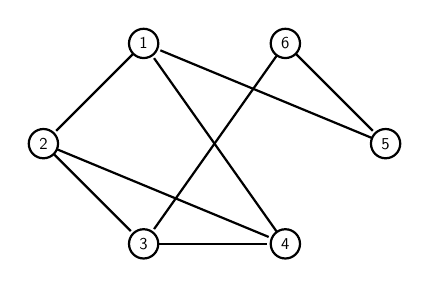
\begin{tikzpicture}[-,>=stealth,shorten >=1pt,auto,node distance=3cm,thick,main node/.style={scale=0.6,circle,draw,font=\sffamily\normalsize}]
                \node[main node] (1) {1};
                \node[main node] (2) [below left of=1] {2};
                \node[main node] (3) [below right of=2] {3};
                \node[main node] (6) [right of=1] {6};
                \node[main node] (5) [below right of=6] {5};
                \node[main node] (4) [below left of=5] {4};
    
                \path[every node/.style={font=\sffamily\small}]
                    (1) edge (2)
                    (2) edge (3)
                    (2) edge (4)
                    (3) edge (4)
                    (4) edge (1)
                    (5) edge (1)
                    (6) edge (3)
                    (6) edge (5)
                    ;
            \end{tikzpicture}

            &\qquad\qquad&
            
            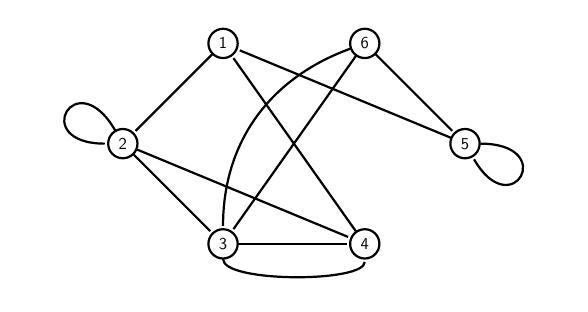
\begin{tikzpicture}[-,>=stealth,shorten >=1pt,auto,node distance=3cm,thick,main node/.style={scale=0.6,circle,draw,font=\sffamily\normalsize}]
                \node[main node] (1) {1};
                \node[main node] (2) [below left of=1] {2};
                \node[main node] (3) [below right of=2] {3};
                \node[main node] (6) [right of=1] {6};
                \node[main node] (5) [below right of=6] {5};
                \node[main node] (4) [below left of=5] {4};
    
                \path[every node/.style={font=\sffamily\small}]
                    (1) edge (2)
                    (2) edge (3)
                    (2) edge (4)
                    (2) edge [loop left, in=180, out=120, min distance=10mm] (2)
                    (3) edge (4)
                    (3) edge [in=-90, out=-90, max distance=3mm] (4)
                    (4) edge (1)
                    (5) edge (1)
                    (5) edge [loop right, in=-60, out=0, min distance=10mm] (5)
                    (6) edge (3)
                    (6) edge [in=90, out=200, min distance=10mm] (3)
                    (6) edge (5)
                    ;
            \end{tikzpicture}
        \end{tabular}
    \end{center}
    
    \begin{frameddefn}{Incidenza e adiacenza}
        Sia $G$ un grafo o un multigrafo. Se $(v_1, v_2) \in E(G)$, allora definiamo l'arco $(v_1,v_2)$ come \textbf{incidente in $v_1$ e $v_2$}, mentre definiamo $v_1$ e $v_2$ come \textbf{adiacenti}
    \end{frameddefn}
    
    \begin{frameddefn}{Grafo non diretto e diretto}

        Sia $G$ un grafo. Diciamo che $G$ è un \textbf{grafo non diretto}, o semplicemente \textit{grafo}, se i suoi archi non possiedono orientamento, ossia se $(u,v) = (v,u)$.
        Altrimenti, diciamo che $G$ è un \textbf{grafo diretto}, o \textit{digrafo}, se i suoi archi possiedono un orientamento, ossia se $(u,v) \neq (v,u)$.
        
    \end{frameddefn}
    
    \textbf{Esempio:}
    \begin{center}
        \begin{tabular}{ccc}
            \textbf{Grafo diretto} && \textbf{Grafo non diretto}\\
            \\
        
            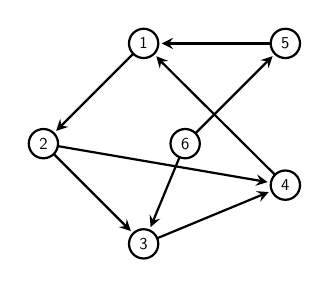
\begin{tikzpicture}[->,>=stealth,shorten >=1pt,auto,node distance=3cm,thick,main node/.style={scale=0.6,circle,draw,font=\sffamily\normalsize}]
                \node[main node] (1) {1};
                \node[main node] (2) [below left of=1] {2};
                \node[main node] (3) [below right of=2] {3};
                \node[main node] (6) [right of=2] {6};
                \node[main node] (5) [above right of=6] {5};
                \node[main node] (4) [below of=5] {4};
    
                \path[every node/.style={font=\sffamily\small}]
                    (1) edge (2)
                    (2) edge (3)
                    (2) edge (4)
                    (3) edge (4)
                    (4) edge (1)
                    (5) edge (1)
                    (6) edge (3)
                    (6) edge (5)
                    ;
            \end{tikzpicture}

            &\qquad\qquad&
            
            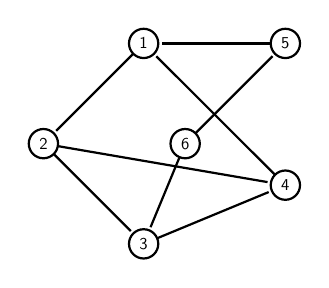
\begin{tikzpicture}[-,>=stealth,shorten >=1pt,auto,node distance=3cm,thick,main node/.style={scale=0.6,circle,draw,font=\sffamily\normalsize}]
                \node[main node] (1) {1};
                \node[main node] (2) [below left of=1] {2};
                \node[main node] (3) [below right of=2] {3};
                \node[main node] (6) [right of=2] {6};
                \node[main node] (5) [above right of=6] {5};
                \node[main node] (4) [below of=5] {4};
    
                \path[every node/.style={font=\sffamily\small}]
                    (1) edge (2)
                    (2) edge (3)
                    (2) edge (4)
                    (3) edge (4)
                    (4) edge (1)
                    (5) edge (1)
                    (6) edge (3)
                    (6) edge (5)
                    ;
            \end{tikzpicture}
        \end{tabular}
    \end{center}
    
    \begin{frameddefn}{Grado di un vertice}
         Dato un grafo o multigrafo $G$ e dato $v \in V(G)$, definiamo come \textbf{grado} di $v$, indicato come $\deg(v)$, il \textbf{numero di archi incidenti} a $v_1$
         
         In particolare, se $G$ è \textbf{diretto}, definiamo come \textbf{grado entrante} di $v$ il numero di archi $(x, v) \in E(G), x \in V(G)$ e come \textbf{grado uscente} di $v$ il numero di archi $(v, y) \in E(G), y \in V(G)$
    \end{frameddefn}
    
    \textbf{Esempio:}
    
    \begin{itemize}
        \item Nel seguente grafo non diretto, si ha che $\deg(4)=2$

        \begin{center}
            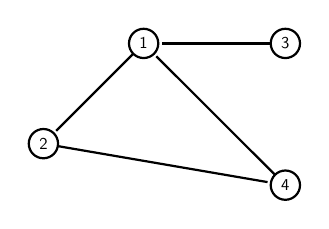
\begin{tikzpicture}[-,>=stealth,shorten >=1pt,auto,node distance=3cm,thick,main node/.style={scale=0.6,circle,draw,font=\sffamily\normalsize}]
                \node[main node] (1) {1};
                \node[main node] (2) [below left of=1] {2};
                \node[main node] (3) [right of=1] {3};
                \node[main node] (4) [below of=3] {4};
    
                \path[every node/.style={font=\sffamily\small}]
                    (1) edge (2)
                    (2) edge (4)
                    (4) edge (1)
                    (3) edge (1)
                    ;
            \end{tikzpicture}
        \end{center}
        
        \newpage
        
        \item Nel seguente grafo diretto, il grado uscente e il grado entrante di $1$ sono rispettivamente pari a $1$ e $2$, dunque si ha che $\deg(1)=3$

        \begin{center}
            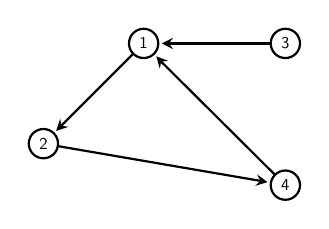
\begin{tikzpicture}[->,>=stealth,shorten >=1pt,auto,node distance=3cm,thick,main node/.style={scale=0.6,circle,draw,font=\sffamily\normalsize}]
                \node[main node] (1) {1};
                \node[main node] (2) [below left of=1] {2};
                \node[main node] (3) [right of=1] {3};
                \node[main node] (4) [below of=3] {4};
    
                \path[every node/.style={font=\sffamily\small}]
                    (1) edge (2)
                    (2) edge (4)
                    (4) edge (1)
                    (3) edge (1)
                    ;
            \end{tikzpicture}
        \end{center}
    \end{itemize}
    
    \begin{framedlem}{Handshaking lemma}
         Dato un grafo $G$ tale che $\abs{E(G)}=m$, si ha che:
         \[\sum_{v \in V(G)} \deg(v) = 2m\]
         Equivalentemente, ogni grafo possiede un numero pari di vertici con grado dispari
    \end{framedlem}
    
    \textit{Dimostrazione:}
    
    \begin{itemize}
        \item Poiché ogni arco $e \in E(G)$ è incidente a due vertici $v_i, v_j \in V(G) \mid v_i \neq v_j$, incrementando di $1$ il grado di entrambi i vertici. Di conseguenza, si vede facilmente che:
         \[\sum_{v \in V(G)} \deg(v) = 2m\]
         $\hfill\qed$
    \end{itemize}
        
    \begin{frameddefn}{Matrice di adiacenza}
        Sia $G$ un grafo avente $n$ vertici, dunque $\abs{V(G)}=n$. Definiamo come \textbf{matrice di adiacenza} una matrice $M \in \mathrm{Mat}_{n \times n}(\{0,1\})$ tale che:
        \[m_{i,j} = \left \{ \begin{array}{ll}
            1 & \text{ se } (v_i, v_j) \in E(G)\\
            0 & \text{ se } (v_i, v_j) \notin E(G)\\
        \end{array}\right .\]
    \end{frameddefn}
    
    \begin{framedprop}{Costi della matrice di adiacenza}
        Sia $G$ dove $\abs{V(G)}=n$ e sia $M \in \mathrm{Mat}_{n \times n}(\{0,1\})$ la sua matrice di adiacenza.
        
        Il \textbf{costo spaziale} di tale matrice è $O(n^2)$, mentre il \textbf{costo computazionale} delle sue operazioni risulta essere:
        \begin{itemize}
            \item Verificare se $(v_i, v_j) \in E(G)$: $O(1)$
            \item Trovare tutti gli adiacenti a $v_i$: $O(n)$
            \item Aggiungere o rimuovere $(v_i, v_j) \in E(G)$: $O(1)$
        \end{itemize}
    \end{framedprop}
    
    \newpage
    
    \textit{Dimostrazione:}
    
    \begin{itemize}
        \item Poiché $M \in  \mathrm{Mat}_{n \times n}(\{0,1\})$, si vede facilmente che il suo costo spaziale sia $O(n^2)$
        \item Inoltre, poiché $(v_i, v_j)\in E(G) \iff m_{i,j} = 1$, è sufficiente leggere il valore dell'entrata $m_{i,j}$ per verificare se $(v_i, v_j) \in E(G)$, rendendo quindi il costo pari a $O(1)$.
        
        Per trovare tutti gli adiacenti di un vertice $v_i$, dunque, è sufficiente leggere il valore delle entrate $m_{i,k}, \forall k \in [0,n]$, rendendo il costo pari a $O(n)$.
        
        \item Nel caso in cui si voglia aggiungere o rimuovere un arco $(v_i, v_j) \in E(G)$, se il grafo è diretto sarà necessario modificare l'entrata $m_{i,j}$, rendendo il costo pari a $O(1)$, mentre se il grafo non è diretto sarà necessario modificare l'entrata $m_{i,j}$ e $m_{j,i}$, rendendo il costo pari a $2 \cdot O(1) = O(1)$
        
        $\hfill\qed$
    \end{itemize}
    
    \begin{frameddefn}{Liste di adiacenza}
        Sia $G$ un grafo avente $n$ vertici, dunque $\abs{V(G)}=n$. Definiamo come \textbf{liste di adiacenza} l'insieme di liste $L_0, \ldots, L_n$ dove $\forall x \in V(G)$ si ha che:
        \[L_x := [v \in V(G) \mid (x, v), (v, x) \in E(G)]\]

        Se $G$ é un \textbf{grafo diretto}, definiamo come \textbf{liste di entrata} l'insieme di liste $L^{in}_0, \ldots, L^{in}_n$ e come \textbf{liste di uscita} l'insieme di liste  $L^{out}_0, \ldots, L^{out}_n$ dove $\forall x \in V(G)$ si ha che:
        \[L^{in}_x := [v \in V(G) \mid (v, x) \in E(G)]\]
        \[L^{out}_x := [v \in V(G) \mid (x, v) \in E(G)]\]
    \end{frameddefn}
    
    \begin{framedprop}{Costi delle liste di adiacenza}
        Sia $G$ dove $\abs{V(G)}=n$ e siano $L_0, \ldots, L_n$ le sue liste di adiacenza.
        
        Il \textbf{costo spaziale} necessario per tutte le liste è $O(n+m)$, dove $\abs{E(G)} =m$, mentre il \textbf{costo computazionale} delle sue operazioni risulta essere:
        \begin{itemize}
            \item Verificare se $(v_i, v_j) \in E(G)$: $O(\deg(v_i))$
            \item Trovare tutti gli adiacenti a $v_i$: $O(\deg(v_i))$
            \item Aggiungere o rimuovere $(v_i, v_j) \in E(G)$: $O(\deg(v_i))$
        \end{itemize}
    \end{framedprop}
    
    \textit{Dimostrazione:}
    
    \begin{itemize}
        
        \item Nel caso in cui $G$ sia un grafo, poiché $(v_i, v_j) \in E(G) \implies (vj, v_i) \in E(G)$, si ha che $\abs{L_i} = \deg(v_i), \forall v_i \in V(G)$. Di conseguenza, il costo spaziale per tutte le liste corrisponderà a:
        \[O \left ( \sum_{v \in V(G)} \deg(v) \right ) = O(2m) = O(m)\]
        
        Inoltre, poiché sono necessari $n$ puntatori ognuno facente riferimento alla testa di una lista di adiacenza, il costo spaziale finale pari a $O(n+m)$
        
        \item Nel caso in cui $G$ sia un grafo diretto, si ha che $\abs{L^{in}_i} = deg_{in}(v_i) \leq \deg(v_i)$ e $\abs{L^{out}_i} = deg_{out}(v_i) \leq \deg(v_i)$, dunque il costo spaziale di entrambe le liste corrisponde $O(\deg(v_i))$. Di conseguenza, il costo spaziale per tutte le liste corrisponderà a:
        \[O \left ( \sum_{v \in V(G)} 2\deg(v) \right ) = O(4m) = O(m)\]
        
        Inoltre, poiché sono necessari $2n$ puntatori ognuno facente riferimento alla testa di una lista di entrata o di uscita, il costo spaziale finale pari a $O(2n+2m) = O(n+m)$

        \item Poiché ognuna delle tre operazioni nel caso peggiore richiede di scorrere l'intera lista di adiacenza, di entrata o di uscita, il costo computazionale di ognuna di esse sarà $O(\deg(v_i))$

        $\hfill\qed$
    \end{itemize}

    \textbf{Esempi:}

    \begin{enumerate}
        \item \begin{itemize}
            \item Consideriamo il seguente grafo
            
            \begin{center}
                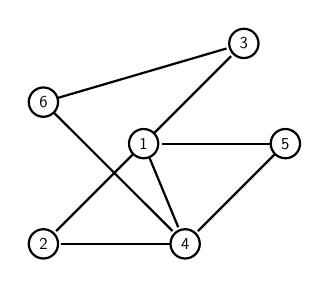
\begin{tikzpicture}[-,>=stealth,shorten >=1pt,auto,node distance=3cm,thick,main node/.style={scale=0.6,circle,draw,font=\sffamily\normalsize}]
                    \node[main node] (1) {1};
                    \node[main node] (2) [below left of=1] {2};
                    \node[main node] (3) [above right of=1] {3};
                    \node[main node] (4) [right of=2] {4};
                    \node[main node] (5) [right of=1] {5};
                    \node[main node] (6) [above of=2] {6};
        
                    \path[every node/.style={font=\sffamily\small}]
                        (1) edge (4)
                        (4) edge (2)
                        (1) edge (2)
                        (1) edge (3)
                        (6) edge (3)
                        (6) edge (4)
                        (5) edge (4)
                        (5) edge (1)
                        ;
                \end{tikzpicture}
            \end{center}

            \item La sua rappresentazione tramite matrice di adiacenza e liste di adiacenza corrisponderà a
            \begin{center}
                \begin{tabular}{ccc}
                    $\begin{array}{c|cccccc}
                        & 1 & 2 & 3 & 4 & 5 & 6\\
                        \hline
                        1 & 0 & 1 & 1 & 1 & 1 & 0\\
                        2 & 1 & 0 & 0 & 1 & 0 & 0\\
                        3 & 1 & 0 & 0 & 0 & 0 & 1\\
                        4 & 1 & 1 & 0 & 0 & 1 & 1\\
                        5 & 1 & 0 & 0 & 1 & 0 & 0\\
                        6 & 0 & 0 & 1 & 1 & 0 & 0
                    \end{array}$

                    &\qquad\qquad\qquad&

                    $\begin{array}{l}
                        1 \to [2,4,3,5]\\
                        2 \to [1,4]\\
                        3 \to [6,1]\\
                        4 \to [2,1,5]\\
                        5 \to [1,4]\\
                        6 \to [4,3]
                    \end{array}$
                \end{tabular}
            \end{center}
        \end{itemize}

        \newpage

        \item \begin{itemize}
            \item Consideriamo il seguente grafo
            
            \begin{center}
                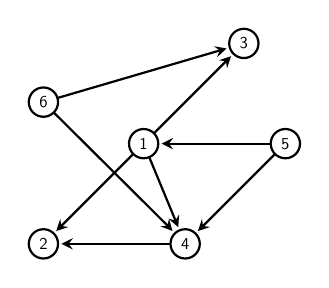
\begin{tikzpicture}[->,>=stealth,shorten >=1pt,auto,node distance=3cm,thick,main node/.style={scale=0.6,circle,draw,font=\sffamily\normalsize}]
                    \node[main node] (1) {1};
                    \node[main node] (2) [below left of=1] {2};
                    \node[main node] (3) [above right of=1] {3};
                    \node[main node] (4) [right of=2] {4};
                    \node[main node] (5) [right of=1] {5};
                    \node[main node] (6) [above of=2] {6};
        
                    \path[every node/.style={font=\sffamily\small}]
                        (1) edge (4)
                        (4) edge (2)
                        (1) edge (2)
                        (1) edge (3)
                        (6) edge (3)
                        (6) edge (4)
                        (5) edge (4)
                        (5) edge (1)
                        ;
                \end{tikzpicture}
            \end{center}

            \item La sua rappresentazione tramite matrice di adiacenza e liste di adiacenza corrisponderà a
            \begin{center}
                \begin{tabular}{ccccc}
                    $\begin{array}{c|cccccc}
                          & 1 & 2 & 3 & 4 & 5 & 6\\
                        \hline
                        1 & 0 & 1 & 1 & 1 & 0 & 0\\
                        2 & 0 & 0 & 0 & 0 & 0 & 0\\
                        3 & 0 & 0 & 0 & 0 & 0 & 0\\
                        4 & 0 & 0 & 0 & 0 & 0 & 0\\
                        5 & 1 & 0 & 0 & 1 & 0 & 0\\
                        6 & 0 & 0 & 1 & 1 & 0 & 0\\
                    \end{array}$

                    &\qquad\qquad&

                    $\begin{array}{l}
                        \text{Entrata}\\
                        \hline
                        1 \to [5]\\
                        2 \to [1,4]\\
                        3 \to [6,1]\\
                        4 \to [2,1,5]\\
                        5 \to [\,]\\
                        6 \to [\,]
                    \end{array}$

                    &\qquad\qquad&

                    $\begin{array}{l}
                        \text{Uscita}\\
                        \hline
                        1 \to [2,4,3]\\
                        2 \to [\,]\\
                        3 \to [\,]\\
                        4 \to [\,]\\
                        5 \to [1,4]\\
                        6 \to [4,3]
                    \end{array}$
                \end{tabular}
            \end{center}
        \end{itemize}
    \end{enumerate}
    
    \quad
    
    \subsection{Passeggiate, tracce, cammini e cicli}
    
    Lo studio della teoria dei grafi deriva da un problema all'apparenza semplice, seppur richiedente un'attenta analisi. Tale problema corrisponde al \textbf{problema dei sette ponti di Königsberg}:
    
    \begin{itemize}
        \item Nella città di Königsberg ci sono sette ponti posizionati nel seguente modo:
        
        \begin{center}
            \includegraphics[scale=0.6]{images/Konigsberg_bridges.png}
        \end{center}
        
        Vogliamo sapere se sia possibile effettuare una passeggiata per la città passando per tutti i ponti  tornando al punto di partenza senza mai passare due volte sullo stesso ponte.
        
        \item A risolvere il problema fu Eulero nel 1736, provando che non sia possibile effettuare un tale tipo di passeggiata. Nella sua dimostrazione, Eulero modellò il problema come un multigrafo, dando origine alla teoria dei grafi:
        
        \begin{center}
            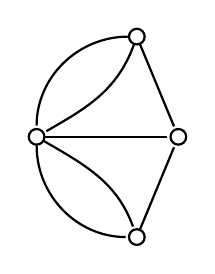
\begin{tikzpicture}[-,>=stealth,shorten >=1pt,auto,node distance=3cm,thick,main node/.style={scale=0.6,circle,draw,font=\sffamily\normalsize}]
                \node[main node] (1) {};
                \node[main node] (2) [below left of=1] {};
                \node[main node] (3) [below right of=2] {};
                \node[main node] (4) [right of=2] {};
    
                \path[every node/.style={font=\sffamily\small}]
                    (1) edge [out=180, in=90] (2)
                    (1) edge [out=-110, in=30] (2)
                    (2) edge [out=270, in=180] (3)
                    (2) edge [out=-30, in=110] (3)
                    (2) edge (4)
                    (1) edge (4)
                    (3) edge (4)
                    ;
            \end{tikzpicture}
        \end{center}
        
        \item In seguito, vedremo la dimostrazione data da Eulero tramite il suo teorema generale
    \end{itemize}
    
    \begin{frameddefn}{Passeggiata}
        Dato un grafo $G$, definiamo come \textbf{passeggiata} una sequenza alternata di vertici $v_1, \ldots, v_k \in V(G)$ ed archi $e_1,\ldots,e_k \in E(G)$, dove $e_i = (v_{i-1}, v_i)$.
        
        In altre parole, definiamo la seguente sequenza come passeggiata:
        \[v_0e_1v_1\ldots v_{i-1}e_iv_i\ldots v_{k-1}e_kv_k\]
    \end{frameddefn}

    \begin{frameddefn}{Traccia e Cammino}
        Sia $G$ un grafo. Definiamo una passeggiata in $G$ come:
        \begin{itemize}
            \item \textbf{Traccia} se tale passeggiata \textbf{non contiene archi ripetuti}
            \item \textbf{Cammino} se tale passeggiata \textbf{non contiene vertici ripetuti} (e di conseguenza neanche archi ripetuti)
        \end{itemize}
    \end{frameddefn}

    \textbf{Esempi:}

    \begin{itemize}
        \item Consideriamo il seguente grafo
        
        \begin{center}
            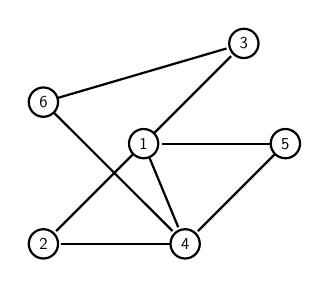
\begin{tikzpicture}[-,>=stealth,shorten >=1pt,auto,node distance=3cm,thick,main node/.style={scale=0.6,circle,draw,font=\sffamily\normalsize}]
                \node[main node] (1) {1};
                \node[main node] (2) [below left of=1] {2};
                \node[main node] (3) [above right of=1] {3};
                \node[main node] (4) [right of=2] {4};
                \node[main node] (5) [right of=1] {5};
                \node[main node] (6) [above of=2] {6};

                \path[every node/.style={font=\sffamily\small}]
                    (1) edge (4)
                    (4) edge (2)
                    (1) edge (2)
                    (1) edge (3)
                    (6) edge (3)
                    (6) edge (4)
                    (5) edge (4)
                    (5) edge (1)
                    ;
            \end{tikzpicture}
        \end{center}

        \item La seguente sequenza è una passeggiata su tale grafo
        \[1-(1,2)-2-(2,4)-4-(4,5)-5-(5,4)-4-(4,1)-1\]

        \item La seguente sequenza è una traccia su tale grafo
        \[4-(4,5)-5-(5,1)-1-(1,2)-2-(2,4)-4-(4,1)-1\]

        \item La seguente sequenza è un cammino su tale grafo
        \[4-(4,5)-5-(5,1)-1-(1,2)-2-(2,4)-4\]
    \end{itemize}

    \begin{frameddefn}{Visita di un vertice}
        Sia $G$ un grafo. Dato $v \in V(G)$, definiamo un vertice $v' \in V(G)$ \textbf{visitabile} da $v$, indicato come $v \to v'$, se esiste una passeggiata da $v$ a $v'$
    \end{frameddefn}

    \begin{framedobs}{}
        Dato un grafo $G$ si ha che:
        \[\exists \text{ una passeggiata } \mid  x \to y \text{ in } G \iff \exists \text{ un cammino } \mid x \to y \text{ in } G\]
    \end{framedobs}

    \begin{frameddefn}{Grafo connesso e fortemente connesso}
        Sia $G$ un grafo. Definiamo $G$ come \textbf{connesso} se
        \[\forall v_1, v_2 \in V(G), \exists \text{ un cammino } \mid  v_1 \to v_2 \lor v_2 \to v_1\]

        Definiamo invece $G$ come \textbf{fortemente connesso} se
        \[\forall v_1, v_2 \in V(G), \exists \text{ due cammini } \mid v_1 \to v_2 \land v_2 \to v_1\]
    \end{frameddefn}


    \textbf{Esempio:}
    \begin{center}
        \begin{tabular}{ccccc}
            \textbf{Fortemente connesso} && \textbf{Connesso} && \textbf{Non connesso}\\
            \\
        
            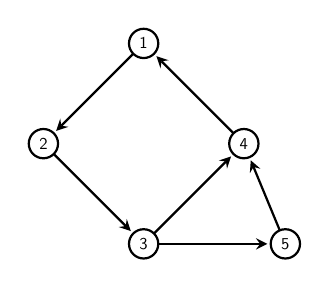
\begin{tikzpicture}[->,>=stealth,shorten >=1pt,auto,node distance=3cm,thick,main node/.style={scale=0.6,circle,draw,font=\sffamily\normalsize}]
                \node[main node] (1) {1};
                \node[main node] (2) [below left of=1] {2};
                \node[main node] (3) [below right of=2] {3};
                \node[main node] (4) [below right of=1] {4};
                \node[main node] (5) [right of=3] {5};
    
                \path[every node/.style={font=\sffamily\small}]
                    (1) edge (2)
                    (2) edge (3)
                    (3) edge (4)
                    (4) edge (1)
                    (5) edge (4)
                    (3) edge (5)
                    ;
            \end{tikzpicture}

            &\qquad\quad&
            
            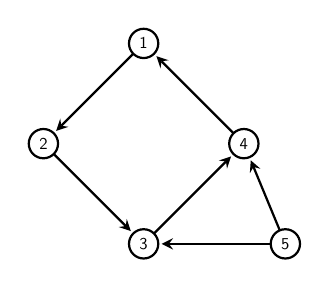
\begin{tikzpicture}[->,>=stealth,shorten >=1pt,auto,node distance=3cm,thick,main node/.style={scale=0.6,circle,draw,font=\sffamily\normalsize}]
                \node[main node] (1) {1};
                \node[main node] (2) [below left of=1] {2};
                \node[main node] (3) [below right of=2] {3};
                \node[main node] (4) [below right of=1] {4};
                \node[main node] (5) [right of=3] {5};
    
                \path[every node/.style={font=\sffamily\small}]
                    (1) edge (2)
                    (2) edge (3)
                    (3) edge (4)
                    (4) edge (1)
                    (5) edge (4)
                    (5) edge (3)
                    ;
            \end{tikzpicture}


            &\qquad\quad&

            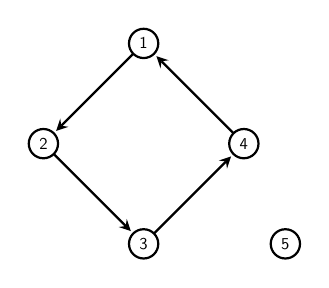
\begin{tikzpicture}[->,>=stealth,shorten >=1pt,auto,node distance=3cm,thick,main node/.style={scale=0.6,circle,draw,font=\sffamily\normalsize}]
                \node[main node] (1) {1};
                \node[main node] (2) [below left of=1] {2};
                \node[main node] (3) [below right of=2] {3};
                \node[main node] (4) [below right of=1] {4};
                \node[main node] (5) [right of=3] {5};
    
                \path[every node/.style={font=\sffamily\small}]
                    (1) edge (2)
                    (2) edge (3)
                    (3) edge (4)
                    (4) edge (1)
                    ;
            \end{tikzpicture}

        \end{tabular}
    \end{center}

    \begin{framedobs}{}
        Un \textbf{grafo non diretto} è \textbf{connesso} se e solo se è \textbf{fortemente connesso}
    \end{framedobs}

    \begin{frameddefn}{Passeggiata chiusa ed aperta}
        Sia $G$ un grafo. Definiamo una passeggiata $v_0e_1\ldots e_kv_k$ su $G$ come \textbf{chiusa} se $v_0 = v_k$, altrimenti essa viene definita \textbf{aperta}
    \end{frameddefn}

    \begin{frameddefn}{Passeggiata Euleriana}
        Sia $G$ un grafo. Definiamo una passeggiata come \textbf{euleriana} se tale passeggiata contiene tutti gli archi in $E(G)$ ed ogni arco è presente una sola volta.

        In altre parole, una passeggiata euleriana è una traccia contenente tutti gli archi in $E(G)$
    \end{frameddefn}

    \begin{framedthm}{Teorema di Eulero}
        Dato un grafo $G$, esiste una passeggiata euleriana chiusa in $G$ se e solo se $G$ è connesso e il grado di ogni vertice è pari:
        \[\exists \text{ passeggiata euleriana chiusa in } G \iff \left \{ \begin{array}{l}
            \forall v_1, v_2 \in V(G), \exists v_1 \to v_2\\
            \forall v \in V(G), \exists k \in \mathbb{Z} \mid \deg(v)=2k
            \end{array} \right .\]
    \end{framedthm}

    \textit{Dimostrazione (implicazione $\impliedby$ omessa):}
    \begin{itemize}
        \item Supponiamo per assurdo che esista una passeggiata euleriana chiusa in $G$ e che $\exists v \in V \mid \deg(v) = 2k+1, \exists k \in \mathbb{Z}$, ossia che esista un vertice avente grado dispari.
        
        \item In tal caso, una volta effettuata la $2k+1$ esima visita su $v$ utilizzando ogni volta un diverso arco incidente ad esso, non sarebbe possibile raggiungere un altro vertice $x \in V(G) \mid (v,x) \in E(G)$ senza necessariamente riutilizzare uno degli archi incidenti a $v$, contraddicendo l'ipotesi per cui tale passeggiata sia euleriana e chiusa.
        
        \item Supponiamo quindi per assurdo che esista una passeggiata euleriana chiusa in $G$ e che $G$ non sia connesso. In tal caso, ne seguirebbe automaticamente che tale passeggiata non possa essere euleriana, poiché esisterebbe un vertice sconnesso avente un arco non utilizzabile nella passeggiata
        
        $\hfill\qed$
    \end{itemize}
    
    \begin{frameddefn}{Ciclo}
        Sia $G$ un grafo. Definiamo come \textbf{ciclo} una \textbf{passeggiata chiusa} dove solo il \textbf{primo} e l'\textbf{ultimo} vertice sono ripetuti.

        Se $G$ è un grafo diretto aciclico, definiamo $G$ come \textbf{DAG (Directed Acyclic Graph)}
    \end{frameddefn}

    \textbf{Esempio:}
    \begin{itemize}
        \item La passeggiata $1 - (1,2) - 2 - (2,3) - 3 - (3,4) - 4 - (4,1) - 1$ è un ciclo in $G$
        \begin{center}
            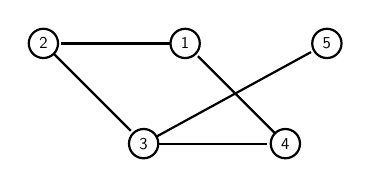
\begin{tikzpicture}[-,>=stealth,shorten >=1pt,auto,node distance=3cm,thick,main node/.style={scale=0.6,circle,draw,font=\sffamily\normalsize}]
                \node[main node] (1) {1};
                \node[main node] (2) [left of=1] {2};
                \node[main node] (3) [below right of=2] {3};
                \node[main node] (4) [below right of=1] {4};
                \node[main node] (5) [right of=1] {5};
    
                \path[every node/.style={font=\sffamily\small}]
                    (1) edge (2)
                    (2) edge (3)
                    (3) edge (4)
                    (4) edge (1)
                    (3) edge (5)
                    ;
            \end{tikzpicture}
        \end{center}
    \end{itemize}

    \section{Depth-first Search (DFS)}

    \begin{frameddefn}{Depth-first Search (DFS)}
        Sia $G $ un grafo. Dato un vertice iniziale $x \in V(G)$ definiamo come \textbf{depth-first search (DFS)} un \textbf{criterio di visita} su $G$ basato sul procedere \textbf{in profondità}, ossia dando precedenza ai vertici più lontani dal vertice iniziale, raggiungendo ogni vertice \textbf{una ed una sola volta}, tornando al vertice precedente \underline{se e solo se} non è più possibile procedere in profondità tramite il vertice attuale, ossia quando tutti i vertici adiacenti sono già stati visitati
    \end{frameddefn}

    \textbf{Esempio:}

    \begin{itemize}
        \item Consideriamo il seguente grafo.
        
        \begin{center}
            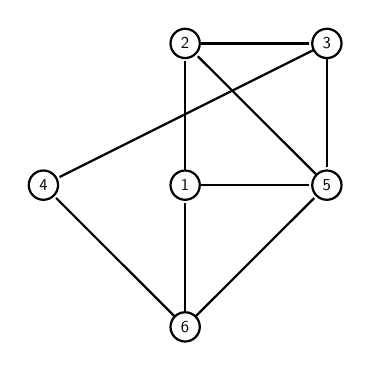
\begin{tikzpicture}[-,>=stealth,shorten >=1pt,auto,node distance=3cm,thick,main node/.style={scale=0.6,circle,draw,font=\sffamily\normalsize}]
                \node[main node] (1) {1};
                \node[main node] (2) [above of=1] {2};
                \node[main node] (3) [right of=2] {3};
                \node[main node] (4) [left of=1] {4};
                \node[main node] (5) [right of=1] {5};
                \node[main node] (6) [below of=1] {6};
    
                \path[every node/.style={font=\sffamily\small}]
                    (1) edge (2)
                    (2) edge (3)
                    (3) edge (4)
                    (3) edge (5)
                    (6) edge (4)
                    (6) edge (5)
                    (6) edge (1)
                    (1) edge (5)
                    (5) edge (2)
                    ;
            \end{tikzpicture}
        \end{center}

        \quad

        \item Scelto $6$ come vertice iniziale, selezioniamo casualmente uno dei tre archi incidenti a $6$, ripetendo tale procedimento finché non sia più possibile scendere in profondità 
    \end{itemize}

    \quad

    \begin{center}
        \begin{tabular}{ccccc}
            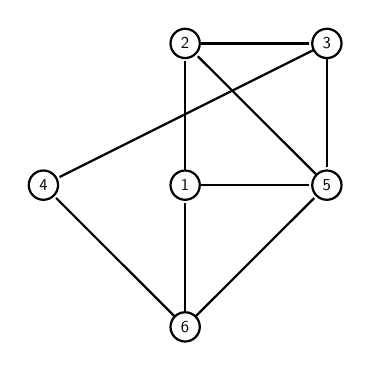
\begin{tikzpicture}[-,>=stealth,shorten >=1pt,auto,node distance=3cm,thick,main node/.style={scale=0.6,circle,draw,font=\sffamily\normalsize}]
                \node[main node] (1) {1};
                \node[main node] (2) [above of=1] {2};
                \node[main node] (3) [right of=2] {3};
                \node[main node] (4) [left of=1] {4};
                \node[main node] (5) [right of=1] {5};
                \node[main node] (6) [below of=1] {6};
    
                \path[every node/.style={font=\sffamily\small}]
                    (1) edge (2)
                    (2) edge (3)
                    (3) edge (4)
                    (3) edge (5)
                    (6) edge (4)
                    (6) edge (5)
                    (6) edge (1)
                    (1) edge (5)
                    (5) edge (2)
                    ;
            \end{tikzpicture}

            &\qquad\quad&

            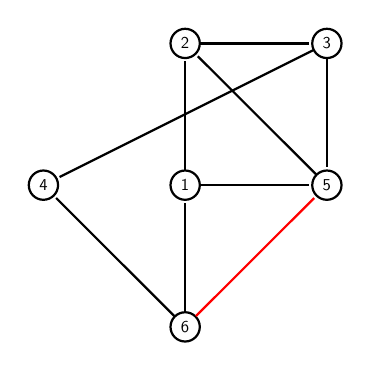
\begin{tikzpicture}[-,>=stealth,shorten >=1pt,auto,node distance=3cm,thick,main node/.style={scale=0.6,circle,draw,font=\sffamily\normalsize}]
                \node[main node] (1) {1};
                \node[main node] (2) [above of=1] {2};
                \node[main node] (3) [right of=2] {3};
                \node[main node] (4) [left of=1] {4};
                \node[main node] (5) [right of=1] {5};
                \node[main node] (6) [below of=1] {6};

                \path[every node/.style={font=\sffamily\small}]
                    (1) edge (2)
                    (2) edge (3)
                    (3) edge (4)
                    (3) edge (5)
                    (6) edge (4)
                    (6) edge (1)
                    (1) edge (5)
                    (5) edge (2)
                    ;
                \draw
                (6) [color=red] edge (5)
                ;
            \end{tikzpicture}

            &\qquad\quad&

            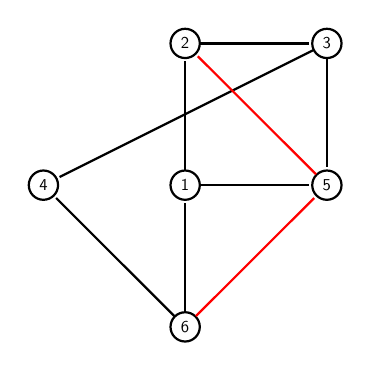
\begin{tikzpicture}[-,>=stealth,shorten >=1pt,auto,node distance=3cm,thick,main node/.style={scale=0.6,circle,draw,font=\sffamily\normalsize}]
                \node[main node] (1) {1};
                \node[main node] (2) [above of=1] {2};
                \node[main node] (3) [right of=2] {3};
                \node[main node] (4) [left of=1] {4};
                \node[main node] (5) [right of=1] {5};
                \node[main node] (6) [below of=1] {6};

                \path[every node/.style={font=\sffamily\small}]
                    (1) edge (2)
                    (2) edge (3)
                    (3) edge (4)
                    (3) edge (5)
                    (6) edge (4)
                    (6) edge (1)
                    (1) edge (5)
                    ;
                \draw
                (6) [color=red] edge (5)
                (5) [color=red] edge (2)
                ;
            \end{tikzpicture}
        \end{tabular}
    \end{center}

    \begin{center}
        \begin{tabular}{ccc}
            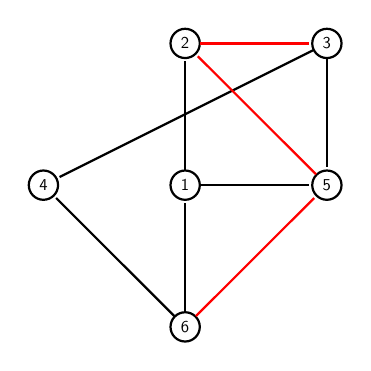
\begin{tikzpicture}[-,>=stealth,shorten >=1pt,auto,node distance=3cm,thick,main node/.style={scale=0.6,circle,draw,font=\sffamily\normalsize}]
                \node[main node] (1) {1};
                \node[main node] (2) [above of=1] {2};
                \node[main node] (3) [right of=2] {3};
                \node[main node] (4) [left of=1] {4};
                \node[main node] (5) [right of=1] {5};
                \node[main node] (6) [below of=1] {6};
    
                \path[every node/.style={font=\sffamily\small}]
                    (1) edge (2)
                    (3) edge (4)
                    (3) edge (5)
                    (6) edge (4)
                    (6) edge (1)
                    (1) edge (5)
                    ;
                \draw
                    (6) [color=red] edge (5)
                    (5) [color=red] edge (2)
                    (2) [color=red] edge (3)
                    ;
            \end{tikzpicture}

            &\qquad\quad&

            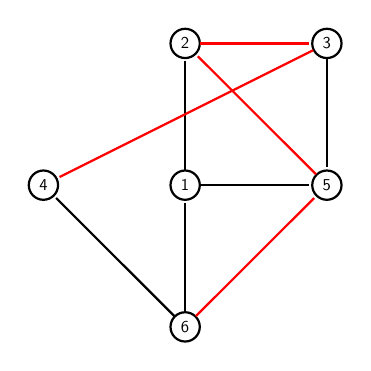
\begin{tikzpicture}[-,>=stealth,shorten >=1pt,auto,node distance=3cm,thick,main node/.style={scale=0.6,circle,draw,font=\sffamily\normalsize}]
                \node[main node] (1) {1};
                \node[main node] (2) [above of=1] {2};
                \node[main node] (3) [right of=2] {3};
                \node[main node] (4) [left of=1] {4};
                \node[main node] (5) [right of=1] {5};
                \node[main node] (6) [below of=1] {6};

                \path[every node/.style={font=\sffamily\small}]
                    (1) edge (2)
                    (3) edge (5)
                    (6) edge (4)
                    (6) edge (1)
                    (1) edge (5)
                    ;
                \draw
                (6) [color=red] edge (5)
                (5) [color=red] edge (2)
                (2) [color=red] edge (3)
                (3) [color=red] edge (4)
                ;
            \end{tikzpicture}
        \end{tabular}
    \end{center}

    \begin{itemize}
        \item Una volta raggiunto il vertice $4$, non è più possibile scendere il profondità poiché tutti i vertici adiacenti a $4$ sono già stati visitati, tornando quindi al vertice $3$ (ossia quello precedente), per cui tuttavia vale lo stesso ragionamento, tornando quindi al vertice $2$, per cui la ricerca DFS è in grado di procedere in profondità poiché il vertice $1$ non è ancora stato visitato

        \begin{center}
            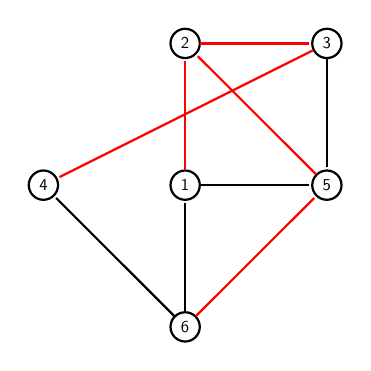
\begin{tikzpicture}[-,>=stealth,shorten >=1pt,auto,node distance=3cm,thick,main node/.style={scale=0.6,circle,draw,font=\sffamily\normalsize}]
                \node[main node] (1) {1};
                \node[main node] (2) [above of=1] {2};
                \node[main node] (3) [right of=2] {3};
                \node[main node] (4) [left of=1] {4};
                \node[main node] (5) [right of=1] {5};
                \node[main node] (6) [below of=1] {6};

                \path[every node/.style={font=\sffamily\small}]
                    (3) edge (5)
                    (6) edge (4)
                    (6) edge (1)
                    (1) edge (5)
                    ;
                \draw
                (6) [color=red] edge (5)
                (5) [color=red] edge (2)
                (2) [color=red] edge (3)
                (3) [color=red] edge (4)
                (1) [color=red] edge (2)
                ;
            \end{tikzpicture}
        \end{center}

        \item A questo punto, tutti i vertici del grafo sono stati visitati, implicando che la ricerca termini risalendo le chiamate ricorsive (dunque tornando a $2$, $5$ e $6$). L'ordine finale di visita finale, dunque , corrisponde a $6,5,2,3,4,1$
    \end{itemize}


    \begin{framedalgo}{Depth-first Search}
        Sia $G $ un grafo e sia $x \in V(G)$ un vertice. Il seguente algoritmo effettua una DFS, restituendo l'insieme di vertici visitabili dalla vertice iniziale $x$

        Il \textbf{costo} risulta essere $O(n^2)$, dove $\abs{V(G)}=n$
    \end{framedalgo}

    \begin{algorithm}[H]
        \caption{Depth-first Search}\label{alg:dfs}
        \KwIn{\\
        G: grafo, $x\in V(G)$}
        \KwOut{\\
        Vertici visitabili da $x$}

        \Fn{\texttt{\upshape DFS(G, x):}}{
            \texttt{Vis = $\{x\}$}\;
            \texttt{\textbf{Stack} S = $\varnothing$}\;
            \texttt{S.push($x$)}\;
            \While{\texttt{S $\neq \varnothing$}}{
                \texttt{$y$ = S.top()}\;
                \eIf{$\exists z \in V(G) \mid (y,z) \in E(G), z \notin $ Vis}{
                    \texttt{S.push($z$)}\;
                    \texttt{Vis.add($z$)}\;
                }
                {
                    \texttt{S.pop()}\;
                }
            }
            \texttt{return Vis}\;
        }
    \end{algorithm}

    \textit{Dimostrazione correttezza algoritmo:}

    \begin{itemize}
        \item Sia $y \in V(G)$ un vertice visitabile da $x$ tramite una passeggiata. Di conseguenza, esiste anche un cammino $v_0e_1v_1\ldots v_{k-1}e_kv_k$ tale che $x \to y$, implicando quindi che $x := v_0$ e $y:= v_k$.
        \item Supponiamo per assurdo che venga raggiunta l'iterazione del while per cui $S = \varnothing$ e che $y \notin \texttt{Vis}$.
        
        \item Sia $v_i$ il vertice di tale cammino avente indice maggiore dove $v_i \in \texttt{Vis}$, implicando che $v_{i+1} \notin \texttt{Vis}$. Se tale vertice esistesse, esso verrebbe tolto dallo stack prima che il vertice $v_{i+1}$ sia visitato dall'algoritmo, poiché $v_{i+1} \notin \texttt{Vis}, \exists (v_i, v_{i+1}) \in E(G)$ e $v_{i+1} \neq v_j, \forall j \in [0,i]$, implicando quindi che l'algoritmo abbia sbagliato l'esecuzione.
        
        \item Di conseguenza, l'unica possibilità è che una volta raggiunta l'iterazione del while per cui $S = \varnothing$ si abbia che $y \in \texttt{Vis}$
        
        $\hfill\qed$
    \end{itemize}

    \textit{Dimostrazione costo dell'algoritmo:}

    \begin{itemize}
        \item Nel caso peggiore in cui $\forall v \in V(G)-\{x\}$ si abbia che $x \to v$, il ciclo while verrebbe eseguito un totale di $2n-1$ volte, poiché ogni vertice, eccetto la vertice iniziale, verrebbe aggiunto e rimosso dallo stack $2$ volte, dando vita a due scenari:
        \begin{itemize}
            \item Se $G$ fosse rappresentato attraverso una matrice di adiacenza, la ricerca del vertice successivo ad ogni iterazione avrebbe un costo pari a $O(n)$, poiché potenzialmente verrebbe analizzata l'intera riga associata al vertice attuale, rendendo il costo del ciclo while pari a $O((2n-1)n) = O(2n^2-n) = O(n^2)$
            \item Se $G$ fosse rappresentato attraverso liste di adiacenza, la ricerca del vertice successivo ad ogni iterazione avrebbe un costo pari a $O(n-1)=O(n)$, poiché,assumendo il caso peggiore, la sua lista di adiacenza associata al vertice attuale conterrebbe ogni vertice del grafo eccetto se stesso, rendendo l'intera riga, rendendo potenzialmente necessario scorrere l'intera lista. Di conseguenza, il costo del ciclo while pari sarebbe pari a $O((2n-1)n) = O(2n^2-n) = O(n^2)$
        \end{itemize}
    \end{itemize}

    \newpage

    \begin{framedalgo}{Depth-first Search (Ottimizzata)}
        Sia $G $ un grafo con liste di adiacenza e sia $x \in V(G)$ un vertice. Il seguente algoritmo effettua una DFS, restituendo l'insieme di vertici visitabili dalla radice $x$

        Il \textbf{costo} risulta essere $O(n+m)$, dove $\abs{V(G)}=n$ e $\abs{E(G)}=m$
    \end{framedalgo}

    \begin{algorithm}[H]
        \caption{Depth-first Search (Ottimizzata)}\label{alg:dfs2}
        \KwIn{\\
        G: grafo, $x \in V(G)$: vertice iniziale}
        \KwOut{\\
        Vertici visitabili da $x$}

        \Fn{\texttt{\upshape DFS\_Optimized(G,x):}}{
            \texttt{Vis = $\{x\}$}\;
            \texttt{\textbf{Stack} S = $\varnothing$}\;
            \texttt{S.push($x$)}\;
            \While{\texttt{S} $\neq \varnothing$}{
                \texttt{$y$ = S.top()}\;
                \While{\texttt{$y$.uscenti $\neq \varnothing$}}{
                    \texttt{$z$ = $y$.uscenti[0]}\;
                    \texttt{$y$.uscenti.remove(0)}\;
                    \If{$z \notin \texttt{Vis}$}{
                        \texttt{Vis.add($z$)}\;
                        \texttt{S.push($z$)}\;
                        \texttt{\textbf{break}}\;
                    }
                }
                \If{\texttt{$y$ == S.top()}}{
                    \texttt{S.pop()}\;
                }
            }
            \texttt{return Vis}\;
        }
    \end{algorithm}

    \textit{Dimostrazione costo dell'algoritmo:}

    \begin{itemize}
        \item Analogamente alla versione non ottimizzata, nel caso in cui $\forall v \in V(G), \exists (x,v) \in E(G)$, il ciclo while verrà eseguito $2n-1$ volte.
        \item Ogni volta che un vertice viene analizzato come potenziale vertice successivo, esso viene rimosso dalla lista di adiacenza del vertice attuale, diminuendo la dimensione di quest'ultima, implicando che il numero totale di controlli effettuati corrisponda esattamente al numero di archi presenti nel grafo, ossia $\abs{E(G)=m}$
        \item Di conseguenza, il costo totale del ciclo while sarà $O(2n-1+m) = O(n+m)$.
        
        $\hfill\qed$
    \end{itemize}

    \newpage

    \begin{framedalgo}{Depth-first Search (Ottimizzata e Ricorsiva)}
        Sia $G $ un grafo con liste di adiacenza e sia $x \in V(G)$ un vertice. Il seguente algoritmo effettua ricorsivamente una DFS, restituendo l'insieme di vertici visitabili da $x$

        Il \textbf{costo} risulta essere $O(n+m)$, dove $\abs{V(G)}=n$ e $\abs{E(G)}=m$
    \end{framedalgo}

    \begin{algorithm}[H]
        \caption{Depth-first Search (Ottimizzata e Ricorsiva)}\label{alg:dfs3}
        \KwIn{\\
        G: grafo, $x \in V(G)$: vertice iniziale}
        \KwOut{\\
        Vertici visitabili da $x$}

        \Fn{\texttt{\upshape DFS\_recursive(G, x, Vis)}:}{
            \For{\texttt{$y \in x$.uscenti}}{
                \If{\texttt{$y \notin$ Vis}}{
                    \texttt{Vis.add($y$)}\;
                    \texttt{DFS\_recursive(G, $y$, Vis)}\;
                }
            }
        }
        \Fn{\texttt{\upshape DFS(G,x)}}{
            \texttt{Vis = \{$x$\}}\;
            \texttt{DFS\_recursive(G, $x$, Vis)}\;
            \texttt{return Vis}\;
        }
    \end{algorithm}

    \textit{Dimostrazione correttezza e costo algoritmo:}

    \begin{itemize}
        \item Analogamente alla DFS ottimizzata, tramite il ciclo for vengono analizzati solo una ed una volta tutti gli archi uscenti dell'attuale vertice $x$, applicando automaticamente le operazioni di rimozione degli archi, richiamando la ricorsione solamente sui vertici mai visitati prima
        \item Inoltre, nonostante non sia presente una vera struttura dati, lo stack è stato "nascosto" sfruttando le chiamate ricorsive (in particolare, utilizzando lo stack della memoria di sistema), ottenendo lo stesso effetto della versione iterativa
        
        \item Per i motivi sopraelencati, il costo dell'algoritmo risulta essere $O(n+m)$
        
        $\hfill\qed$
    \end{itemize}

    \newpage

    \subsection{Albero ed Arborescenza}

    \quad

    \begin{frameddefn}{Albero e Arborescenza}
        Definiamo un grafo non diretto $T$ come \textbf{albero} se $\forall x,y \in V(T)$ esiste un solo cammino tale che $x \to y$ e $y \to x$ passante per gli stessi vertici.

        Definiamo un grafo diretto $A$ come \textbf{arborescenza} se dato un vertice $x \in V(A)$, detto \textbf{radice}, si ha che $\forall y \in V(A)$ esiste un solo cammino tale che $x \to y$
    \end{frameddefn}

    \begin{center}
        \begin{tabular}{ccc}
            \textbf{Albero} && \textbf{Arborescenza con radice 6}\\\\

            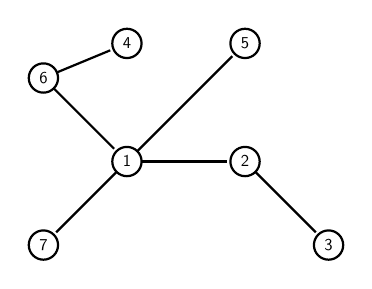
\begin{tikzpicture}[-,>=stealth,shorten >=1pt,auto,node distance=2.5cm,thick,main node/.style={scale=0.6,circle,draw,font=\sffamily\normalsize}]
                \node[main node] (1) {1};
                \node[main node] (2) [right of=1] {2};
                \node[main node] (3) [below right of=2] {3};
                \node[main node] (4) [above of=1] {4};
                \node[main node] (5) [above of=2] {5};
                \node[main node] (6) [above left of=1] {6};
                \node[main node] (7) [below left of=1] {7};

                \path[every node/.style={font=\sffamily\small}]
                    (6) edge (1)
                    (6) edge (4)
                    (1) edge (5)
                    (1) edge (2)
                    (2) edge (3)
                    (1) edge (7)
                ;
            \end{tikzpicture}

            &\qquad\qquad&

            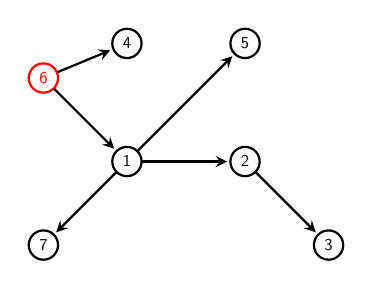
\begin{tikzpicture}[->,>=stealth,shorten >=1pt,auto,node distance=2.5cm,thick,main node/.style={scale=0.6,circle,draw,font=\sffamily\normalsize}]
                \node[main node] (1) {1};
                \node[main node] (2) [right of=1] {2};
                \node[main node] (3) [below right of=2] {3};
                \node[main node] (4) [above of=1] {4};
                \node[main node] (5) [above of=2] {5};
                \node[main node] (6) [color=red, above left of=1] {6};
                \node[main node] (7) [below left of=1] {7};

                \path[every node/.style={font=\sffamily\small}]
                    (6) edge (1)
                    (6) edge (4)
                    (1) edge (5)
                    (1) edge (2)
                    (2) edge (3)
                    (1) edge (7)
                ;
            \end{tikzpicture}
        \end{tabular}
    \end{center}

    \begin{framedobs}{}
        Sia $G$ un grafo. Dato un vertice $x \in V(G)$, il \textbf{sotto-grafo} $H \subseteq G$ generato dall'insieme di archi e vertici percorsi da una DFS avente $x$ come vertice iniziale corrisponde a:
        \begin{itemize}
            \item Un albero radicato (se $G$ non è diretto), detto \textbf{albero di visita}
            \item Un'arborescenza (se $G$ è diretto), detta \textbf{arborescenza di visita}
        \end{itemize}
    \end{framedobs}
    \textbf{Esempio:}

    \begin{itemize}
        \item Dato il seguente grafo
        
        \begin{center}
            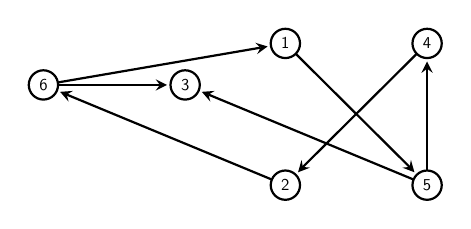
\begin{tikzpicture}[->,>=stealth,shorten >=1pt,auto,node distance=3cm,thick,main node/.style={scale=0.6,circle,draw,font=\sffamily\normalsize}]
                \node[main node] (1) {1};
                \node[main node] (2) [below of=1] {2};
                \node[main node] (3) [above left of=2] {3};
                \node[main node] (4) [right of=1] {4};
                \node[main node] (5) [below of=4] {5};
                \node[main node] (6) [left of=3] {6};

                \path[every node/.style={font=\sffamily\small}]
                    (5) edge (3)
                    (6) edge (3)
                    (6) edge (1)
                    (1) edge (5)
                    (2) edge (6)
                    (5) edge (4)
                    (4) edge (2)
                    ;
                \draw
                ;
            \end{tikzpicture}
        \end{center}

        \quad
        
        due sue arborescenze di visita corrispondono a:
    \end{itemize}

    \begin{center}
        \begin{tabular}{ccc}

            \textbf{Arborescenza di visita su 6} & & \textbf{Arborescenza di visita su 5}\\\\

            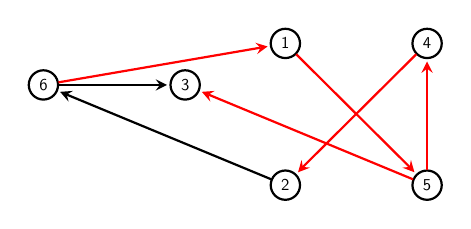
\begin{tikzpicture}[->,>=stealth,shorten >=1pt,auto,node distance=3cm,thick,main node/.style={scale=0.6,circle,draw,font=\sffamily\normalsize}]
                \node[main node] (1) {1};
                \node[main node] (2) [below of=1] {2};
                \node[main node] (3) [above left of=2] {3};
                \node[main node] (4) [right of=1] {4};
                \node[main node] (5) [below of=4] {5};
                \node[main node] (6) [left of=3] {6};

                \path[every node/.style={font=\sffamily\small}]
                    (6) edge (3)
                    (2) edge (6)
                    ;
                
                \path[every node/.style={font=\sffamily\small}]
                    [color=red]
                    (6) edge (1)
                    (1) edge (5)
                    (5) edge (3)
                    (5) edge (4)
                    (4) edge (2)
                ;
            \end{tikzpicture}
            
            &\qquad\qquad&

            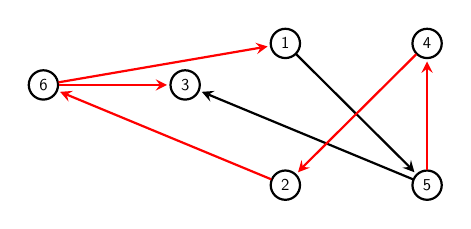
\begin{tikzpicture}[->,>=stealth,shorten >=1pt,auto,node distance=3cm,thick,main node/.style={scale=0.6,circle,draw,font=\sffamily\normalsize}]
                \node[main node] (1) {1};
                \node[main node] (2) [below of=1] {2};
                \node[main node] (3) [above left of=2] {3};
                \node[main node] (4) [right of=1] {4};
                \node[main node] (5) [below of=4] {5};
                \node[main node] (6) [left of=3] {6};

                \path[every node/.style={font=\sffamily\small}]
                    (1) edge (5)
                    (5) edge (3)
                ;
                \path[every node/.style={font=\sffamily\small}]
                    [color=red]
                    (6) edge (3)
                    (5) edge (4)
                    (4) edge (2)
                    (2) edge (6)
                    (6) edge (1)
                ;
            \end{tikzpicture}
        \end{tabular}
    \end{center}

    \begin{framedprop}{}
        Dato un grafo $G$, se $G$ è un \textbf{albero} o \textbf{arborescenza}, allora $\abs{E(G)} = \abs{V(G)}-1$
    \end{framedprop}

    \textit{Dimostrazione:}

    \begin{itemize}
        \item Sia $G$ un albero o arborescenza avente $V(G) = n$ nodi 
        \item Supponiamo per assurdo che $E(G) > n-1$. In tal caso, esisterebbero necessariamente almeno due archi $(x,y), (z,y) \in E(G) \mid (x,y) \neq (z,y)$ ed un vertice $w \in V(G) \mid w \to x, w \to z$ (dove $w$ è la radice nel caso in cui $G$ sia un'arborescenza), tramite cui ottenere due cammini $w \to y$, contraddicendo l'ipotesi per cui $G$ sia un albero o arborescenza. Dunque necessariamente si ha che $E(G) \leq n-1$.
        \item Supponiamo ora per assurdo che $E(G) < n-1$. In tal caso, esisterebbe necessariamente almeno un vertice $v  \in V(G)$ non connesso a $G$, implicando che non possa esistere alcun cammino verso tale vertice (escludendo il cammino nullo $v \to v$).  Dunque necessariamente si ha che $E(G) \geq n-1$, contraddicendo l'ipotesi per cui $G$ sia un albero o arborescenza.
        \item Di conseguenza, concludiamo che $E(G) = n-1$
        
        $\hfill\qed$
    \end{itemize}

    \quad

    \subsection{Tempi di visita, di chiusura e classificazione degli archi}

    \quad

    \begin{frameddefn}{Tempi di visita e Tempo di chisura}
        Sia $G$ un grafo e sia $C$ un \textbf{contatore} inizializzato a 0 inserito all'interno dell'algoritmo DFS, il quale viene \textbf{incrementato ogni volta che viene visitato un nuovo vertice}.

        Per ogni vertice $v \in V(G)$, definiamo come:
        
        \begin{itemize}
            \item \textbf{Tempo di visita di $v$}, indicato come \textbf{$t(v)$}, il valore assunto da $C$ nell'istante in cui $v$ viene aggiunto allo stack
            \item \textbf{Tempo di chiusura di $v$}, indicato come \textbf{$T(v)$}, il valore assunto da $C$ nell'istante in cui $v$ viene rimosso dallo stack
            \item \textbf{Intervallo di visita di $v$} l'intervallo $Int(v) := [t(v), T(v)]$
        \end{itemize}
    \end{frameddefn}


    \newpage

    \textbf{Esempio:}

    \begin{itemize}
        \item Consideriamo il seguente multigrafo:
        
        \begin{center}
            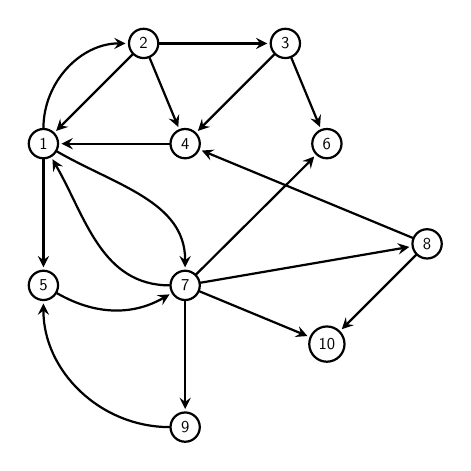
\begin{tikzpicture}[->,>=stealth,shorten >=1pt,auto,node distance=3cm,thick,main node/.style={scale=0.6,circle,draw,font=\sffamily\normalsize}]
                \node[main node] (1) {1};
                \node[main node] (2) [above right of=1]{2};
                \node[main node] (3) [right of=2]{3};
                \node[main node] (4) [right of=1]{4};
                \node[main node] (5) [below of=1]{5};
                \node[main node] (6) [right of=4]{6};
                \node[main node] (7) [below of=4]{7};
                \node[main node] (8) [below right of=6]{8};
                \node[main node] (9) [below of=7]{9};
                \node[main node] (10) [below left of=8]{10};

                \path[every node/.style={font=\sffamily\small}]
                    (1) edge [out=90, in=180] (2)
                    (1) edge (5)
                    (1) edge [out=-30, in=90] (7)
                    (2) edge (1)
                    (2) edge (3)
                    (2) edge (4)
                    (3) edge (4)
                    (3) edge (6)
                    (4) edge (1)
                    (7) edge [out=180, in=-60] (1)
                    (7) edge (6)
                    (7) edge (8)
                    (7) edge (9)
                    (7) edge (10)
                    (5) edge [out=-30, in=210] (7)
                    (8) edge (4)
                    (8) edge (10)
                    (9) edge [out=180, in=270] (5)
                    ;
            \end{tikzpicture}
        \end{center}

        \item Effettuando una DFS avente come vertice iniziale il vertice $1$, una delle possibili arborescenze generate e il suo corrispettivo insieme di intervalli di visita corrisponde a:
        
        \begin{center}
            \begin{tabular}{ccc}
                \begin{tabular}{c}
                    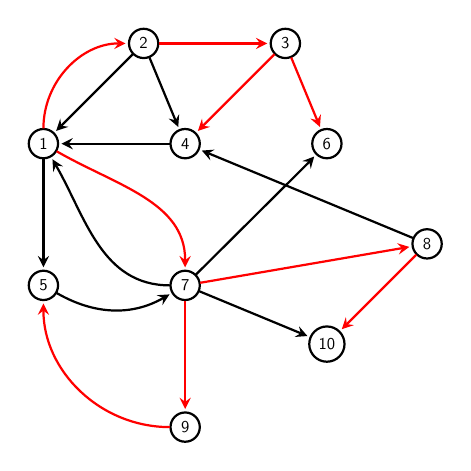
\begin{tikzpicture}[->,>=stealth,shorten >=1pt,auto,node distance=3cm,thick,main node/.style={scale=0.6,circle,draw,font=\sffamily\normalsize}]
                        \node[main node] (1) {1};
                        \node[main node] (2) [above right of=1]{2};
                        \node[main node] (3) [right of=2]{3};
                        \node[main node] (4) [right of=1]{4};
                        \node[main node] (5) [below of=1]{5};
                        \node[main node] (6) [right of=4]{6};
                        \node[main node] (7) [below of=4]{7};
                        \node[main node] (8) [below right of=6]{8};
                        \node[main node] (9) [below of=7]{9};
                        \node[main node] (10) [below left of=8]{10};
        
                        \path[every node/.style={font=\sffamily\small}]
                            (1) edge (5)
                            (2) edge (1)
                            (2) edge (4)
                            (4) edge (1)
                            (7) edge [out=180, in=-60] (1)
                            (7) edge (6)
                            (7) edge (10)
                            (5) edge [out=-30, in=210] (7)
                            (8) edge (4)
                            ;
        
                        \path[every node/.style={font=\sffamily\small}]
                            [color=red]
                            (1) edge [out=90, in=180] (2)
                            (1) edge [out=-30, in=90] (7)
                            (2) edge (3)
                            (3) edge (4)
                            (3) edge (6)
                            (7) edge (8)
                            (7) edge (9)
                            (8) edge (10)
                            (9) edge [out=180, in=270] (5)
                            ;
                    \end{tikzpicture}
                \end{tabular}
            
                &\qquad\qquad&

                \begin{tabular}{c|cc}
                    \textbf{v}& $\textbf{t(v)}$ & $\textbf{T(v)}$\\
                    \hline
                    \textbf{1} & 1 & 10 \\
                    \textbf{2} & 2 & 5  \\
                    \textbf{3} & 3 & 5  \\
                    \textbf{4} & 5 & 5  \\
                    \textbf{5} & 10& 10 \\
                    \textbf{6} & 4 & 4  \\
                    \textbf{7} & 6 & 10 \\
                    \textbf{8} & 7 & 8  \\
                    \textbf{9} & 9 & 10 \\
                    \textbf{10}& 8 & 8  \\
                \end{tabular}
            \end{tabular}
        \end{center}
    \end{itemize}

    \begin{framedprop}{}
        Sia $G$ un grafo. Dato un arco $(u,v) \in E(G)$, dove $u$ è detto \textbf{coda} e $v$ è detto \textbf{testa}, solo una delle seguenti condizioni è verificata:
        \begin{itemize}
            \item $Int(u) \subseteq Int(v)$
            \item $Int(u) \supseteq Int(v)$
            \item $Int(u) \cap Int(v) = \varnothing$
        \end{itemize} 
    \end{framedprop}

    \textit{Dimostrazione:}

    \begin{itemize}
        \item Per definizione stessa, si ha che $t(u) \leq T(u)$ e $t(v) \leq T(v)$
        \item Consideriamo quindi i sei casi possibili:
        \begin{itemize}
            \item $t(u) < t(v) \leq T(u) \leq T(v)$
            \item $t(v) < t(u) \leq T(v) \leq T(u)$
            \item $t(u) < t(v) \leq T(v) \leq T(u)$
            \item $t(v) < t(u) \leq T(u) \leq T(v)$
            \item $t(u) \leq T(u) < t(v) \leq T(v)$
            \item $t(v) \leq T(v) < t(u) \leq T(u)$
        \end{itemize}

        \item Per quanto riguarda gli ultimi quattro casi, notiamo facilmente che:
        \begin{itemize}
            \item $t(u) < t(v) \leq T(v) \leq T(u) \implies Int(u) \supseteq Int(v)$
            \item $t(v) < t(u) \leq T(u) \leq T(v) \implies Int(u) \subseteq Int(v)$
            \item $t(u) \leq T(u) < t(v) \leq T(v) \implies Int(u) \cap Int(v) = \varnothing$
            \item $t(v) \leq T(v) < t(u) \leq T(u) \implies Int(u) \cap Int(v) = \varnothing$
        \end{itemize}

        \item Supponiamo quindi per assurdo che $t(u) < t(v) \leq T(u) \leq T(v)$, ossia che i due intervalli si intersechino, ma nessuno dei due è interamente contenuto dell'altro.
        
        Poiché $t(u) < t(v)$, ne segue che $u$ sia stato aggiunto allo stack prima di $v$. Di conseguenza, è impossibile che $u$ sia stato tolto dallo stack prima di $v$, contraddicendo l'ipotesi per cui $T(u) \leq T(v)$.

        \item Con un ragionamento del tutto analogo, possiamo dimostrare che anche $t(v) < t(u) \leq T(v) \leq T(u)$ sia un caso impossibile
        \item Di conseguenza, concludiamo che le uniche possibilità siano:
        \begin{itemize}
            \item $Int(u) \subseteq Int(v)$
            \item $Int(u) \supseteq Int(v)$
            \item $Int(u) \cap Int(v) = \varnothing$
        \end{itemize} 

        $\hfill\qed$
    \end{itemize}

    \begin{frameddefn}{Classificazione degli archi di visita}
        Sia $G $ un grafo e sia $A $ un'arborescenza generata da una DFS su $G$. Per ogni arco di $G$ \textbf{non appartenente all'arborescenza}, dunque $\forall (u,v) \in E(G) - E(A)$, definiamo tale arco come:
        \begin{itemize}
            \item \textbf{Arco all'indietro (back edge)} se l'intervallo della coda è contenuto in quello della testa, ossia se $Int(u) \subseteq Int(v)$ 
            \item \textbf{Arco in avanti (forward edge)} se l'intervallo della testa è contenuto in quello della coda, ossia se $Int(u) \supseteq Int(v)$ 
            \item \textbf{Arco di attraversamento (cross edge)} se l'intervallo della testa è disgiunto con l'intervallo della coda, ossia se $Int(u) \cap Int(v) = \varnothing$
        \end{itemize}
    \end{frameddefn}

    \newpage

    \textbf{Esempio:}

    \begin{itemize}
        \item Riprendiamo l'arborescenza generata nell'esempio precedente

        \begin{center}
            \begin{tabular}{ccc}
                \begin{tabular}{c}
                    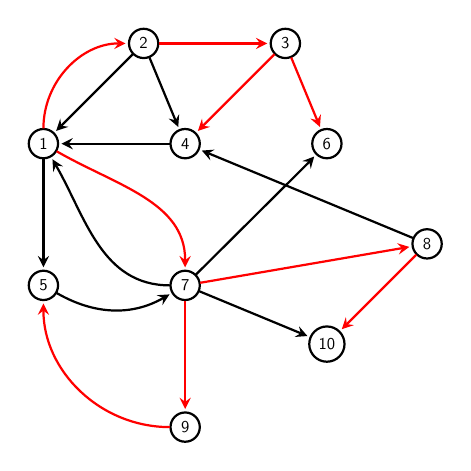
\begin{tikzpicture}[->,>=stealth,shorten >=1pt,auto,node distance=3cm,thick,main node/.style={scale=0.6,circle,draw,font=\sffamily\normalsize}]
                        \node[main node] (1) {1};
                        \node[main node] (2) [above right of=1]{2};
                        \node[main node] (3) [right of=2]{3};
                        \node[main node] (4) [right of=1]{4};
                        \node[main node] (5) [below of=1]{5};
                        \node[main node] (6) [right of=4]{6};
                        \node[main node] (7) [below of=4]{7};
                        \node[main node] (8) [below right of=6]{8};
                        \node[main node] (9) [below of=7]{9};
                        \node[main node] (10) [below left of=8]{10};
        
                        \path[every node/.style={font=\sffamily\small}]
                            (1) edge (5)
                            (2) edge (1)
                            (2) edge (4)
                            (4) edge (1)
                            (7) edge [out=180, in=-60] (1)
                            (7) edge (6)
                            (7) edge (10)
                            (5) edge [out=-30, in=210] (7)
                            (8) edge (4)
                            ;
        
                        \path[every node/.style={font=\sffamily\small}]
                            [color=red]
                            (1) edge [out=90, in=180] (2)
                            (1) edge [out=-30, in=90] (7)
                            (2) edge (3)
                            (3) edge (4)
                            (3) edge (6)
                            (7) edge (8)
                            (7) edge (9)
                            (8) edge (10)
                            (9) edge [out=180, in=270] (5)
                            ;
                    \end{tikzpicture}
                \end{tabular}
            
                &\qquad\qquad&

                \begin{tabular}{c|cc}
                    \textbf{v}& $\textbf{t(v)}$ & $\textbf{T(v)}$\\
                    \hline
                    \textbf{1} & 1 & 10 \\
                    \textbf{2} & 2 & 5  \\
                    \textbf{3} & 3 & 5  \\
                    \textbf{4} & 5 & 5  \\
                    \textbf{5} & 10& 10 \\
                    \textbf{6} & 4 & 4  \\
                    \textbf{7} & 6 & 10 \\
                    \textbf{8} & 7 & 8  \\
                    \textbf{9} & 9 & 10 \\
                    \textbf{10}& 8 & 8  \\
                \end{tabular}
            \end{tabular}
        \end{center}

        \item Classifichiamo quindi gli archi non appartenenti all'arborescenza:
        \begin{itemize}
            \item L'arco $(2,1)$ è un back edge (blu), poiché $[2,5] \subseteq [1,10]$ 
            \item L'arco $(2,4)$ è un forward edge (verde), poiché $[2,5] \supseteq [5,5]$ 
            \item L'arco $(7,6)$ è un cross edge (nero), poiché $[6,10] \cap [4,4] = \varnothing$
            \item $\ldots$
        \end{itemize}
        
        \begin{center}
            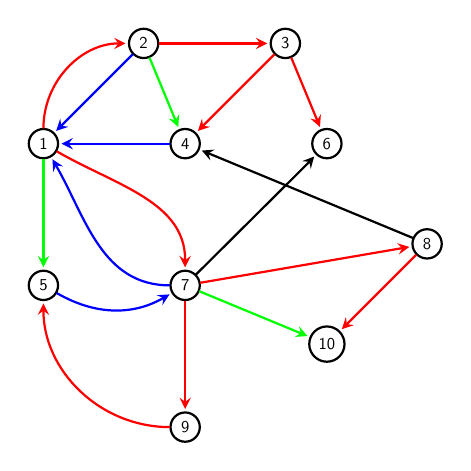
\begin{tikzpicture}[->,>=stealth,shorten >=1pt,auto,node distance=3cm,thick,main node/.style={scale=0.6,circle,draw,font=\sffamily\normalsize}]
                \node[main node] (1) {1};
                \node[main node] (2) [above right of=1]{2};
                \node[main node] (3) [right of=2]{3};
                \node[main node] (4) [right of=1]{4};
                \node[main node] (5) [below of=1]{5};
                \node[main node] (6) [right of=4]{6};
                \node[main node] (7) [below of=4]{7};
                \node[main node] (8) [below right of=6]{8};
                \node[main node] (9) [below of=7]{9};
                \node[main node] (10) [below left of=8]{10};

                \path[every node/.style={font=\sffamily\small}]
                    (7) edge (6)
                    (8) edge (4)
                    ;

                \path[every node/.style={font=\sffamily\small}]
                    [color=red]
                    (1) edge [out=90, in=180] (2)
                    (1) edge [out=-30, in=90] (7)
                    (2) edge (3)
                    (3) edge (4)
                    (3) edge (6)
                    (7) edge (8)
                    (7) edge (9)
                    (8) edge (10)
                    (9) edge [out=180, in=270] (5)
                    ;

                \path[every node/.style={font=\sffamily\small}]
                    [color=green]
                    (2) edge (4)
                    (1) edge (5)
                    (7) edge (10)
                ;

                \path[every node/.style={font=\sffamily\small}]
                    [color=blue]
                    (2) edge (1)
                    (4) edge (1)
                    (7) edge [out=180, in=-60] (1)
                    (5) edge [out=-30, in=210] (7)
                ;

            \end{tikzpicture}
        \end{center}
    \end{itemize}

    \quad
    
    \begin{framedalgo}{Classificare gli archi di visita}
        Sia $G $ un grafo con liste di adiacenza e sia $x \in V(G)$ un vertice. Il seguente algoritmo effettua una DFS avente $x$ come vertice iniziale, restituendo l'insieme degli archi all'indietro, in avanti e di attraversamento generati.

        Il \textbf{costo} risulta essere $O(n+m)$, dove $\abs{V(G)}=n$ e $\abs{E(G)}=m$
    \end{framedalgo}
    
    \begin{algorithm}[H]
        \caption{Classificare archi generati da una DFS con vertice iniziale $x \in V(G)$}\label{find_edges}
        \KwIn{\\
        G: grafo diretto, x : $x \in V(G)$}
        \KwOut{\\
        Un insieme di back edge, un insieme di forward edge e un insieme di cross edge}

        \Fn{\texttt{\upshape classifyDirectEdges(G, x):}}{
            \texttt{Vis, t, T = [0, ..., 0]} \qquad //n elementi inizializzati a 0\;
            \texttt{Padri = [-1, ..., -1]}\;
            \texttt{\textbf{Stack} S = $\varnothing$}\;
            \texttt{$c$ = 1}\;
            \texttt{Vis[$x$] = 1}\;
            \texttt{S.add($x$)}\;
            \texttt{t[$x$] = $c$}\;
            \texttt{Padri[$x$] = $x$}\;
            \While{\texttt{S $\neq \varnothing$}}{
                \texttt{$y$ = S.top()}\;
                \While{\texttt{$y$.uscenti $\neq \varnothing$}}{
                    \texttt{$z$ = $y$.uscenti[0]}\;
                    \texttt{$y$.uscenti.remove(0)}\;
                    \uIf{\texttt{Vis[$z$] = 0}}{
                        \texttt{Vis[$z$] = 1}\;
                        \texttt{S.push($z$)}\;
                        \texttt{$c++$}\;
                        \texttt{t[$z$] = $c$}\;
                        \texttt{Padri[$z$] = $y$}\;
                        \texttt{\textbf{break}}\;
                    }
                }

                \uIf{\texttt{$y$ == S.top()}}{
                    \texttt{S.pop()}\;
                    \texttt{T[$y$] = $c$}\;
                }
            }
            \texttt{Back, Forward, Cross = $\varnothing$}\;
            \For{$v \in V(G)$}{
                \For{\texttt{$u \in v$.entranti}}{
                    \uIf{\texttt{Padri[$v$] $\neq u$}}{
                        \uIf{\texttt{T[$u$] $<$ t[$v$] $\lor$ T[$v$] $<$ t[$u$]}}{
                            \texttt{Cross.add($(u,v)$)}\;
                        }
                        \uElseIf{\texttt{T[$u$] $\leq$ T[$v$]}}{
                            \texttt{Back.add($(u,v)$)}\;
                        }
                        \uElse{
                            \texttt{Forward.add($(u,v)$)}\;
                        }
                    }
                }
            }
            \texttt{return Back, Forward, Cross}\;
        }
    \end{algorithm}

    \textit{Dimostrazione correttezza algoritmo:}

    \begin{itemize}
        \item In linea di massima, l'algoritmo risulta essere una versione modificata della versione ottimizzata della DFS (algoritmo \ref{alg:dfs2}). In particolare, sono stati aggiunti:
        \begin{itemize}
            \item Un contatore $c$, utilizzato per i tempi di visita
            \item Un'array \texttt{Vis} di $n$ elementi, dove se l'$i$-esimo elemento vale 1 allora il vertice $v_i \in V(G)$ è stato visitato (0 se non visitato)
            \item Un'array \texttt{t}, dove l'$i$-esimo elemento dell'array corrisponde al tempo di visita del vertice $v_i \in V(G)$
            \item Un'array \texttt{T}, dove l'$i$-esimo elemento dell'array corrisponde al tempo di chiusura del vertice $v_i \in V(G)$
            \item Un'array \texttt{Padri}, dove l'$i$-esimo elemento dell'array corrisponde al padre del vertice $v_i \in V(G)$, ossia il vertice $u \in V(G)$ tramite cui è stato raggiunto il vertice $v_i$ nella DFS
        \end{itemize}
        \item Analizziamo quindi il comportamento degli ultimi due cicli for aggiunti:
        \begin{itemize}
            \item Per ogni vertice $v \in V(G)$, vengono considerati tutti i suoi vertici entranti. Di conseguenza, stiamo considerando tutti gli archi $(u,v) \in E(G)$
            \item Sia $A$ l'arborescenza generata dalla DFS. Se \texttt{Padri[v] = u}, allora si ha che $(u,v) \in E(A)$, poiché $v$ è stato visitato tramite $u$ all'interno della DFS. Analogamente, se \texttt{Padri[v] $\neq$ u}, allora si ha che $(u,v) \notin E(A)$, dunque $(u,v)$ dovrà necessariamente essere un arco all'indietro, in avanti o di attraversamento
            \item [If)] Nei casi in cui $T(u) < t(v)$ o $T(v) < t(v)$, ne segue necessariamente che $Int(u) \cap Int(v) = \varnothing$
            \item [Else if)] Se la condizione precedente è falsa (ossia se $T(u) \geq t(v)$ e $T(v) \geq t(v)$) e si verifica che $T(u) \leq T(v)$, ne segue necessariamente che $t(v) < t(u) \leq T(u) \leq T(v) \implies Int(u) \subseteq Int(v)$, implicando che $(u,v)$ sia un arco all'indietro
            \item [Else)] Infine, se $(u,v)$ non è né un arco all'indietro e né di attraversamento, l'unica possibilità è che esso sia un arco in avanti
        \end{itemize}
        $\hfill\qed$
    \end{itemize}

    \textit{Dimostrazione costo computazionale:}
    \begin{itemize}
        \item Il costo dei due cicli for annidati corrisponde a:
        \[\sum_{v \in V(G)} O(1) + O(deg_{in}(v)) = O(n)+O(m) = O(n+m)\]
        mantenendo inalterato il costo della DFS

        $\hfill\qed$
    \end{itemize}


    \begin{framedalgo}{Trovare intervalli di visita (Ricorsivo)}
        Sia $G $ un grafo con liste di adiacenza e sia $x \in V(G)$ un vertice. Il seguente algoritmo effettua ricorsivamente una DFS avente $x$ come vertice iniziale, restituendo gli intervalli di visita di ogni vertice.

        Il \textbf{costo} risulta essere $O(n+m)$, dove $\abs{V(G)}=n$ e $\abs{E(G)}=m$
    \end{framedalgo}

    \begin{algorithm}[H]
        \caption{Trovare gli intervalli di visita generati da una DFS con vertice iniziale $x \in V(G)$ su un grafo diretto $G$}\label{find_intervals}
        \KwIn{\\
        G: grafo diretto, x : $x \in V(G)$}
        \KwOut{\\
        Un insieme di back edge, un insieme di forward edge e un insieme di cross edge}

        \Fn{\texttt{\upshape DFS\_recursive(G, x, Vis, t, T, c)}:}{
            \For{\texttt{$y \in x$.adiacenti}}{
                \If{\texttt{$y \notin$ Vis}}{
                    \texttt{Vis.add($y$)}\;
                    \texttt{$c$.increment()}\;
                    \texttt{t[$y$] = $c$}\;
                    \texttt{DFS\_recursive(G, $y$, Vis, t, T, $c$)}\;
                }
            }
            \texttt{T[$x$] = $c$}\;
        }
        \Fn{\texttt{\upshape getVisitTimes(G,x)}}{
            \texttt{Vis = \{$x$\}}\;
            \texttt{t = [0, ..., 0]} \qquad\qquad //n elementi inizializzati a 0\;
            \texttt{T = [0, ..., 0]}\;
            \texttt{\textbf{Counter} $c$ = 1} \qquad\qquad\,\,\, //oggetto contatore\;
            \texttt{t[$x$] = $c$}\;
            \texttt{DFS\_recursive(G, $x$, Vis, t, T, $c$)}\;
            \texttt{return t, T}\;
        }
    \end{algorithm}

    \textit{Dimostrazione correttezza e costo algoritmo:}
    \begin{itemize}
        \item Poiché sono stati aggiunti solo due array ed un oggetto contatore, il costo e la correttezza risultano essere analoghi alla normale DFS ricorsiva. Dunque, il costo è $O(n+m)$
        
        $\hfill\qed$
    \end{itemize}

    \begin{framedobs}{}
        Se $G $ è un grafo non diretto, \textbf{non vi è distinzione tra arco all'indietro ed arco in avanti}, poiché, non essendo gli archi orientati, non vi è distinzione tra testa e coda. Di conseguenza, \underline{utilizziamo solo il termine arco all'indietro} per indicare entrambe le situazioni
    \end{framedobs}

    \begin{framedprop}{}
        Sia $G $ un grafo non diretto. Dato l'albero di visita $T$ generato da una DFS su $G$, per ogni arco di $(u,v) \in E(G) - E(T)$, si ha che $Int(u) \cap Int(v) \neq \varnothing$

        Di conseguenza, in un \textbf{grafo non diretto non possono esistere cross-edge}
    \end{framedprop}

    \textit{Dimostrazione:}
    \begin{itemize}
        \item Se $t(u) < t(v)$, allora è impossibile che $u$ venga tolto dallo stack prima di $v$, poiché l'arco $(u,v) \in E(G)$ (essendo non diretto) verrebbe obbligatoriamente utilizzato dalla DFS, implicando che $Int(v) \subseteq Int(u)$
        \item Per ragionamento analogo, se $t(v) < t(u)$ otteniamo che $Int(u) \subseteq Int(v)$
        
        $\hfill\qed$
    \end{itemize}

    \begin{framedcor}{}
        Sia $G $ un \textbf{grafo non diretto connesso}. Dato l'albero di visita $T$ generato da una DFS su $G$, ogni arco $(u,v) \in E(G) - E(T)$ è un \textbf{arco all'indietro}
    \end{framedcor}

    \quad

    \section{Studio dei grafi ciclici e aciclici}

    \subsection{Trovare cicli in un grafo}

    \begin{framedthm}[label={cycle_thm_undir}]{Presenza di cicli in un grafo connesso non diretto}
        Dato un \textbf{grafo connesso non diretto} $G$, si ha che:
        \[\forall \text{ DFS su } G,\exists \text{ arco all'indietro in } G \iff \exists \text{ ciclo in } G\]
    \end{framedthm}

    \textit{Dimostrazione:}

    \begin{itemize}
        \item Consideriamo un qualsiasi albero di visita $T$ generato da una DFS su $G$. Poiché $G$ è connesso, ogni vertice è raggiungibile dalla DFS, dunque si ha che $V(T) = V(G)$. Inoltre, poiché anche $T$ è connesso, si ha che $\forall x,y \in V(T)$ esiste un cammino su $T$ tale che $x \to y$ 
        \item Supponiamo quindi che esista un arco all'indietro $(u,v) \in E(G)$ generato da tale DFS, implicando che $(u,v) \notin E(T)$. Poiché $u,v \in V(T)$, ne segue che esisterà un cammino $C$ su $T$ tale che $u \to v$ e $(u,v) \notin C$. Infine, poiché in un grafo diretto si ha che $(u,v) \in E(G) \implies (v,u) \in E(G)$, la passeggiata $C \cup (v,u)$ risulta essere un ciclo.
        \item Viceversa, supponiamo che esista un ciclo in $G$ composto dai vertici $c_0,\ldots, c_k$. Poiché $G$ è connesso, eseguendo una DFS su un qualsiasi vertice $x \in V(G)$, tale DFS dovrà necessariamente visitare almeno una volta ogni vertice $c_0,\ldots, c_k$.
        \item Per comodità, assumiamo che $c_0$ sia il primo vertice appartenente al ciclo ad essere visitato. Una volta raggiunto il vertice $c_k$, l'arco $(c_k, c_0)$ non potrà appartenere all'arborescenza generata, poiché $c_0$ risulta già essere stato visitato.
        \item Dunque, poiché in un grafo non diretto ogni arco ogni arco non appartenente ad un'arborescenza è un arco all'indietro, ne segue che $(c_k,c_0)$ sia un arco all'indietro
        \item Inoltre, poiché $G=T$ e in un albero si ha che $\forall u,v \in V(G)$ esiste un solo cammino non diretto tale che $x \to y$ e $y \to x$, ogni DFS su $G$ genererà l'albero di visita $T$
        
        $\hfill\qed$
    \end{itemize}

    \begin{framedthm}{}
        Un grafo $G$ è \textbf{aciclico connesso e non diretto} se e solo se è un \textbf{albero}.
    \end{framedthm}

    \textit{Dimostrazione:}
    \begin{itemize}
        \item Se $G$ è un grafo aciclico connesso e non diretto, per il teorema precedente si ha che
        \[\nexists \text{ ciclo in } G \iff \exists \text{ DFS in } G \mid \nexists \text{ arco all'indietro in } G\]
        \item Sia quindi $T$ l'albero di visita generato da tale DFS. Poiché $G$ non è diretto e poiché non esistono archi all'indietro, ne segue che ogni arco appartenga necessariamente all'albero di visita, dunque $e \in E(G) \implies e \in E(T)$. Inoltre, poiché per definizione stessa si ha che $f \in E(T) \implies f \in E(G)$, concludiamo che $E(G) = E(T)$, implicando a sua volta che $G = T$
        
        \item Viceversa, se $G$ è un albero allora, per definizione stessa, ne segue che $\forall x,y \in V(G)$ esiste un solo cammino indiretto tale che $x \to y$ e $y \to x$, implicando quindi che $G$ sia connesso ed aciclico
        
        $\hfill\qed$
    \end{itemize}
    
    \begin{framedthm}[label={cycle_thm_dir}]{Presenza di cicli in un grafo connesso diretto}
        Dato un \textbf{grafo connesso diretto} $G$, si ha che:
        \[\exists \text{ DFS su } G \mid \exists \text{ arco all'indietro in } G \iff \exists \text{ ciclo in } G\]
    \end{framedthm}

    \textit{Dimostrazione:}

    \begin{itemize}
        \item Consideriamo una DFS su $G$ in cui viene generato un arco all'indietro $(u,v) \in E(G)$. Sia inoltre $A $ l'arborescenza di visita generata da una DFS tale DFS. 
        \item Poiché $(u,v)$ è un arco all'indietro, ne segue che $t(v) < t(u) \leq T(u) \leq T(v)$, dunque $u$ è stato aggiunto allo stack dopo $v$ e prima che $v$ venisse rimosso, implicando che esista un cammino $C$ tale che $v \to u$.

        Di conseguenza, la passeggiata $C \cup (u,v)$ risulta essere un ciclo

        \item Viceversa, supponiamo che esista un ciclo $c_0,\ldots, c_k$ in $G$ e consideriamo una DFS avente radice $x \in V(G)$ in cui uno dei vertici del ciclo viene visitato (per comodità, supponiamo che venga visitato $c_0$), implicando che anche ogni vertice del ciclo debba essere visitato da tale DFS.
        \item Supponiamo per assurdo che esista un vertice del ciclo $c_i$ con indice minimo $i \in [1,k]$ tale che $c_i$ che non sia stato visitato prima della chisura di $c_0$.
        \item Poiché $c_i$ è stato scelto con indice minimo, ne segue che $c_{i-1}$ sia stato visitato prima della chiusura di $c_0$, implicando che $t(c_0) < t(c_{i-1}) \leq T(c_0)$.
        \item Poiché $t(c_0) < t(c_{i-1}) \leq T(c_0) \leq T(c_{i-1}) \implies Int(c_0) \cap Int(c_{i-1}) \neq \varnothing$ è un caso impossibile, ne segue necessariamente che 
        \[t(c_0) < t(c_{i-1}) \leq T(c_{i-1}) \leq T(c_{0}) \implies Int(c_{i-1}) \subseteq Int(c_0)\] dunque $c_i$ viene chiuso prima della chisura di $c_0$, implicando che la DFS abbia sbagliato a non visitare $c_i$, poiché $c_{i-1} \to c_i$
        \item Dunque, l'unica possibilità è che ogni vertice del ciclo venga visitato prima della chiusura di $c_0$, implicando che $Int(c_j) \subseteq Int(c_0), \forall j \in [1,k]$
        \item In particolare, quindi, ne segue che l'arco $(c_k, c_0) \in E(G)$ risulti essere un arco all'indietro poiché $Int(c_k) \subseteq Int(c_0)$
        
        $\hfill\qed$
    \end{itemize}

    \begin{framedcor}{}
        Dato un \textbf{grafo fortemente connesso diretto} $G$, si ha che:
        \[\forall \text{ DFS su } G, \exists \text{ arco all'indietro in } G \iff \exists \text{ ciclo in } G\]
    \end{framedcor}

    \textit{Dimostrazione:}
    \begin{itemize}
        \item Se $G$ è fortemente connesso, ne segue che i vertici $c_0, \ldots, c_k$ componenti il ciclo vengano raggiunti da ogni DFS, dunque (per dimostrazione analoga alla precedente) l'arco $(c_k, c_0) \in E(G)$ sarà sempre un arco all'indietro
        
        $\hfill\qed$
    \end{itemize}

    \begin{framedalgo}{Trovare un ciclo in un grafo}
        Sia $G$ un grafo rappresentato tramite liste di adiacenza. Il seguente algoritmo restituisce, se esistente, un ciclo in $G$. Il \textbf{costo} risulta essere:
        \begin{itemize}
            \item $O(n)$ se $G$ è non diretto
            \item $O(n+m)$ se $G$ è diretto
        \end{itemize}
        dove $\abs{V(G)}=n$ e $\abs{E(G)} = m$
    \end{framedalgo}

    \begin{algorithm}[H]
        \caption{Trovare un ciclo in un grafo}\label{findCycle_2}
        \KwIn{\\
        G: grafo\\
        }
        \KwOut{\\
        Ciclo in G}

        \Fn{\texttt{\upshape DFS\_Cycle(G, x, c, t, T, Padri, Cycle):}}{

            \texttt{c.increment()}\;
            \texttt{t[$x$] = c}\;
            \For{\texttt{$y \in x$.uscenti}}{
                \uIf{\texttt{Cycle == $\varnothing$}}{
                    \uIf{\texttt{t[$y$] == 0}}{
                        \texttt{Padri[$y$] = $x$}\;
                        \texttt{DFS\_Cycle(G, y, c, t, T, Padri, Cycle)}\;
                    }
                    \uElseIf{\texttt{$y \neq$ Padri[$x$] \textbf{and} T[$y$] == 0}}{
                        \texttt{$z$ = $x$}\;
                        \While{$z \neq y$}{
                            \texttt{Cycle.head\_insert($z$)}\;
                            \texttt{$z$ = Padri[$z$]}\;
                        }
                        \texttt{Cycle.head\_insert($y$)}\;
                    }
                }
            }
            \texttt{T[$x$] = c}\;
        }

        \Fn{\texttt{\upshape findCycle(G)}:}{
            \texttt{t, T = [0, ..., 0]}\;
            \texttt{Padri = [-1, ..., -1]}\;
            \texttt{\textbf{Counter} c = 0}\;
            \texttt{\textbf{List} Cycle = $\varnothing$}\;
            \For{\texttt{$v \in V(G)$}}{
                \uIf{\texttt{Cycle == $\varnothing$ \textbf{and} t[$v$] == 0}}{
                    \texttt{Padri[$v$] = $v$}\;
                    \texttt{DFS\_Cycle(G, y, c, t, T, Padri, Cycle)}\;
                }
            }
            \texttt{return Cycle}\;
        }
    \end{algorithm}

    \textit{Dimostrazione correttezza algoritmo:}

    \begin{itemize}
        \item Sia $x \in V(G)$ il vertice attualmente analizzato dalla DFS e siano $y_0, \ldots, y_k \in V(G)$ i vertici tali che $(x,y_i) \in E(G), $\texttt{t[$y_i$]}$=0, \forall i \in [0,k]$, implicando dunque che $y_0, \ldots, y_k$ siano discendenti di $x$
        \item Sia $y' \in V(G)$ il vertice tale che $(x,y) \in E(G)$, \texttt{t[$y'$]} $\neq 0$ e \texttt{T[$y'$]} $= 0$. Poiché $x$ è il vertice attualmente visitato dalla DFS, ne segue che $t(y) < t(x) \leq T(x)$.
        
        \item Tuttavia, poiché \texttt{T[$y'$]} $= 0$, la visita del vertice $y'$ non è stata ancora conclusa, implicando  necessariamente che
        \[t(y) < t(x) \leq T(x) \leq T(y) \implies (x,y') \text{ è un arco all'indietro}\]
        \item Di conseguenza, ne segue che $y'$ sia un antenato di $x$ e che tutti i vertici $z_0, \ldots, z_h \in V(G)$ aventi come antenato $y$ e come discendente $x$ siano appartenenti al ciclo
        
        $\hfill\qed$
    \end{itemize}

    \textit{Dimostrazione costo algoritmo:}

    \begin{itemize}
        \item Trattandosi di una DFS modificata, ne segue automaticamente che il costo dell'algoritmo sia $O(n+m)$
        \item Supponiamo quindi che $G$ sia non diretto. Poiché il caso peggiore dell'algoritmo viene raggiunto nel caso in cui $G$ sia aciclico, per dimostrazione precedente ne segue necessariamente che $G$ sia un'unione disgiunta di alberi $T_1, \ldots, T_k$ (o un singolo albero $T$ se $G$ è anche connesso)
        \item Di conseguenza, si ha che
        \[m = \abs{E(G)} = \sum_{i=0}^k \abs{E(T_i)} = \sum_{i=0}^k \abs{V(T_i)}-1 \leq V(G) = n \implies m \leq n\]
        implicando dunque che il costo dell'algoritmo sia $O(n+m)=O(n)$

        $\hfill\qed$
    \end{itemize}

    \begin{framedobs}{}
        Se $G$ è un grafo non diretto, è possibile rimuovere dall'algoritmo precedente l'array \texttt{T}, i controlli e le operazioni inerenti ad esso, poiché in $G$ possono esistere solo archi all'indietro.

        Di conseguenza, è sufficiente verificare che $t(y) < t(x)$ affinché $(x,y) \in E(G)$ sia un arco all'indietro
    \end{framedobs}

    \quad

    \subsection{Ordinamenti topologici}

    \quad

    \begin{frameddefn}{Ordinamento topologico}
        Sia $G$ un grafo diretto. Dati i suoi vertici $V(G) = \{v_0, \ldots, v_n\}$, definiamo come \textbf{ordinamento topologico} un ordinamento di tali vertici in cui ogni vertice viene prima di tutti i vertici raggiungibili da un suo arco uscente
    \end{frameddefn}

    \textbf{Esempio:}

    \begin{itemize}
        \item Consideriamo il seguente grafo
        
        \begin{center}
            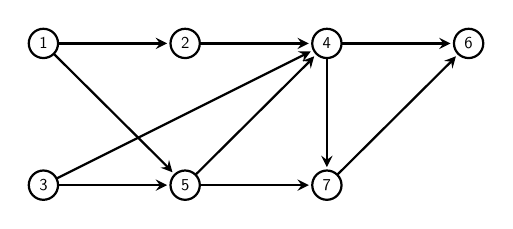
\begin{tikzpicture}[->,>=stealth,shorten >=1pt,auto,node distance=3cm,thick,main node/.style={scale=0.6,circle,draw,font=\sffamily\normalsize}]
                \node[main node] (1) {1};
                \node[main node] (2) [right of=1] {2};
                \node[main node] (3) [below of=1] {3};
                \node[main node] (4) [right of=2] {4};
                \node[main node] (5) [below of=2] {5};
                \node[main node] (6) [right of=4] {6};
                \node[main node] (7) [below of=4] {7};

                \path[every node/.style={font=\sffamily\small}]
                    (1) edge (2)
                    (1) edge (5)
                    (2) edge (4)
                    (3) edge (4)
                    (3) edge (5)
                    (5) edge (7)
                    (5) edge (4)
                    (4) edge (7)
                    (4) edge (6)
                    (7) edge (6)
                    ;
                \draw
                ;
            \end{tikzpicture}
        \end{center}

        \item Le due seguenti sequenze di vertici sono due ordinamenti topologici possibili di tale grafo:
        \begin{itemize}
            \item Precedenza ai vertici più in alto: $1,2,3,5,4,7,6$
            \item Precedenza ai vertici più a sinistra: $1,3,2,5,4,7,6$
        \end{itemize}
    \end{itemize}

    \begin{framedthm}{}
        Dato un grafo diretto $G$, si ha che:
        \[\exists \text{ ordinamento topologico in }G \iff \nexists \text{ ciclo in }G\]
    \end{framedthm}

    \textit{Dimostrazione:}

    \begin{itemize}
        \item Supponiamo per assurdo che esista un ordinamento topologico in $G$ e che esista un ciclo $v_0e_1v_1e_2\ldots e_kv_0$ in $G$, implicando che $v_1$ sia un vertice uscente di $v_0$.
        
        In tal caso, verrebbe contraddetta l'ipotesi per cui in $G$ esiste un ordinamento topologico, poiché $v_0$ verrebbe sia prima di $v_1$ sia dopo $v_1$. Di conseguenza, l'unica possibilità è che non esista alcun ciclo in $G$
        \item Viceversa, supponiamo per assurdo che non esista un ciclo in $G$ e che non esista un ordinamento topologico in $G$, implicando che esista un vertice $v \in V(G)$ tale che $v$ sia raggiungibile da un arco uscente di un vertice $v'$ a sua volta raggiungibile da un arco uscente $v$.
        
        Di conseguenza, si avrebbe che $v \to v' \to v$, contraddicendo l'ipotesi per cui in $G$ non esistano cicli, dunque l'unica possibilità è che in $G$ esista un ordinamento topologico.
        
        $\hfill\qed$
    \end{itemize}

    \begin{framedobs}{}
        Dato un grafo diretto aciclico $G$, si ha che:
        \begin{itemize}
            \item $\exists v \in V(G) \mid deg_{in}(v) = 0$
            \item $\exists v' \in V(G) \mid deg_{out}(v) = 0$
        \end{itemize}
    \end{framedobs}

    \textit{Dimostrazione:}
    \begin{itemize}
        \item Supponiamo per assurdo che $G$ sia un DAG e che $\nexists v \in V(G) \mid deg_{out}(v) = 0$. Poiché $G$ è aciclico, esiste un ordinamento topologico $v_0,\ldots, v_n$ in $G$, dove $\abs{V(G)} = n$.
        
        \item Poiché ogni vertice ha almeno un vertice uscente, per comodità supponiamo che $(v_i, v_{i+1}) \in E(G), \forall i \in [1,n-1]$, implicando quindi che $v_1 \to v_2 \to \ldots \to v_n$
        
        \item Poiché $deg_{out}(v_n) \neq 0$, ne segue che $\exists v_k \in V(G) \mid k \in [0,n-1]$ tale che $(v_n, v_k) \in E(G)$. Di conseguenza, esiste un ciclo in $G$ tale che $v_k \to v_n \to v_k$, contraddicendo l'ipotesi per cui $G$ sia aciclico.
        
        \item Seguendo un ragionamento analogo, dimostriamo che se si avesse $\nexists v \in V(G) \mid deg_{in}(v) = 0$ si otterrebbe una contraddizione
        \item Di conseguenza, l'unica possibilità è che $deg_{in}(v_0)=0$ e $deg_{out}(v_n)=0$
        
        $\hfill\qed$
    \end{itemize}

    \begin{framedalgo}{Trovare un ordinamento topologico}
        Sia $G$ un DAG. Il seguente algoritmo restituisce un ordinamento topologico di $G$

        Il \textbf{costo computazionale} di tale algoritmo è $O(n(n+m))$, dove $\abs{V(G)}=n$ e $\abs{E(G)}=m$, se $G$ è rappresentato tramite liste di adiacenza
    \end{framedalgo}

    \begin{algorithm}[H]
        \caption{Trovare un ordinamento topologico in un DAG}\label{ord_top_1}
        \KwIn{\\
        G: grafo diretto aciclico}
        \KwOut{\\
        Ordinamento topologico in G}
        \Fn{\texttt{\upshape findTopologicalSorting(G):}}{
            \texttt{\textbf{List} L = $\varnothing$}\;
            \While{$V(G) \neq \varnothing$}{
                \texttt{$v$ = $v \in V(G) \mid deg_{out}(v) = 0$}\;
                \texttt{L.head\_insert($v$)}\;
                \texttt{$G$.remove($v$)}\;
            }
            \texttt{return L}\;
        }
    \end{algorithm}

    \newpage

    \textit{Dimostrazione correttezza algoritmo:}

    \begin{itemize}
        \item Siano $G_0,\ldots,G_k$ le istanze del grafo $G$ ad ogni iterazione del ciclo while. Poiché $G$ è aciclico, ne segue che anche $G_0,\ldots, G_k$ siano aciclici, poiché rimuovere vertici non crea cicli in tali grafi.
        \item Per l'osservazione precedente, dunque $\forall i \in [0,n]$ si ha che $\exists v_i \in V_i(G_i) \mid deg_{out}(v_i)=0 \mid $ implicando che ad ogni iterazione esista sempre un vertice selezionabile finché $V(G) \neq \varnothing$. Di conseguenza, si ha che $k = \abs{V(G)}$.
        \item Notiamo inoltre che, ad ogni rimozione di un vertice $x \in V(G)$, per ogni vertice $y \in V(G) \mid (y, x) \in E(G)$ il valore di $deg_{out}(y)$ venga decrementato di uno
        \item Sia quindi $L := v_0,\ldots, v_k$ l'output del programma. Supponiamo per assurdo che $L$ non sia un ordinamento topologico, implicando che $\exists v_i,v_j \in L$ tali che $(v_i, v_j) \in E(G)$ e $v_j$ venga prima di $v_i$ nell'ordinamento (dunque $v_j$ è più a sinistra di $v_i$).
        
        \item In tal caso, l'algoritmo avrebbe sbagliato a selezionare $v_i$, poiché $(v_i, v_j) \in E(G) \implies deg_{out}(v_i) > 0$.  Di conseguenza, l'unica possibilità è che tali vertici non esistano, implicando quindi che $L$ sia un ordinamento topologico
        
        $\hfill\qed$
    \end{itemize}

    \textit{Dimostrazione costo dell'algoritmo:}
    \begin{itemize}
        \item Come dimostrato nella correttezza dell'algoritmo, il ciclo while viene iterato sempre $\abs{V(G)}=n$ volte.
        \item L'inserimento in testa nella lista risulta avere un costo pari a $O(1)$, mentre la rimozione del nodo da $G$ risulta avere un costo pari a $O(n+m)$, poiché nel caso peggiore è necessario rimuovere dalle liste di tutti i nodi gli archi entranti o uscenti verso il nodo rimosso.
        \item Il costo interno del ciclo while, dunque, risulta essere $O(n+m)$, venendo eseguito $n$ volte per un costo totale di  $n \cdot O(n+m) = O(n(n+m))$

        $\hfill\qed$
    \end{itemize}

    \begin{framedobs}{}
        Sia $G $ un DAG connesso. Dato $(u,v) \in E(G)$, si ha che $t(v) \leq T(v) \leq T(u)$
    \end{framedobs}

    \textit{Dimostrazione:}
    \begin{itemize}
        \item Sia $A$ l'arborescenza generata da una DFS su $G$. Se $(u,v) \in E(A)$, ne segue automaticamente che $t(u) < t(v) \leq T(v) \leq T(u)$
        
        \item Consideriamo quindi $(u,v) \in E(G)-E(A)$. Essendo $G$ un DAG, per il Teorema della \nameref{cycle_thm_dir} si ha che:
        \[\nexists \text{ ciclo in } G \iff \exists \text{ DFS in } G \mid \nexists \text{ arco all'indietro in } G\]
        
        \item Di conseguenza, l'unica possibilità è che $(u,v) \in E(G)-E(T)$ sia un arco in avanti o di attraversamento:
        \begin{itemize}
            \item $Int(u) \supseteq Int(v) \implies t(u) < t(v) \leq T(v) \leq T(u)$
            \item $Int(u) \cap Int(v) = \varnothing \implies t(v) \leq T(v) < t(u) \leq T(u)$
        \end{itemize}

        $\hfill\qed$
    \end{itemize}

    \begin{framedalgo}{Trovare un ordinamento topologico (Ottim.)}
        Sia $G $ un DAG rappresentato tramite liste di adiacenza. Il seguente algoritmo restituisce un possibile ordinamento topologico di $G$.

        Il \textbf{costo} risulta essere $O(n+m)$, dove $\abs{V(G)}=n$ e $\abs{E(G)}=m$
    \end{framedalgo}

    \begin{algorithm}[H]
        \caption{Trovare un ordinamento topologico in un DAG}\label{ord_top_2}
        \KwIn{\\
        G: grafo diretto aciclico connesso}
        \KwOut{\\
        Ordinamento topologico in G}

        \Fn{\texttt{\upshape DFS\_Ord(G, u, Vis, L):}}{
            \texttt{Vis.add(u)}\;
            \For{\texttt{$v \in u$.uscenti}}{
                \uIf{$v \notin$ \texttt{Vis}}{
                    \texttt{DFS\_Ord(G, v, Vis, L)}\;
                }
            }
            \texttt{L.head\_insert($u$)}\;
        }


        \Fn{\texttt{\upshape findTopologicalSorting\_2(G):}}{
            \texttt{\textbf{List} L = $\varnothing$}\;
            \texttt{Vis = $\varnothing$}\;
            \For{$u \in V$}{
                \uIf{$u \notin$ \texttt{Vis}}{
                    \texttt{recursive\_DFS\_ord(G, u, Vis, L)}\;
                }
            }
            \texttt{return L}\;
        }

    \end{algorithm}

    \textit{Dimostrazione correttezza e costo algoritmo:}
    \begin{itemize}
        \item Consideriamo gli archi $(u,v) \in E(G)$ generati in \texttt{recursive\_DFS\_ord()}. Poiché $G$ è un DAG, per l'osservazione precedente si ha che $t(v) \leq T(v) \leq T(u)$. 
        
        Di conseguenza, ordinando i vertici in modo che il loro tempo di chiusura sia decrescente, svolto implicitamente dalla ricorsione appendendo il vertice attualmente analizzato all'inizio della lista, otteniamo un ordine topologico, poiché ogni vertice uscente $v$ verrà inserito in testa prima del vertice attuale $u$
        \item Consideriamo quindi gli elementi $L_{i} := u_{i}, \ldots, v_k$ aggiunti dal vertice $u_1$ all'iterazione $i$-esima del ciclo for di \texttt{findTopologicalSorting\_2()}. Nel caso in cui esista un arco $(v_i, v_{i+1}) \in E(G) \mid v_i \in L_{i}, v_{i+1} \in L_{i+1}$, si ha che
        \[(v_i, v_{i+1}) \implies t(v_{i+1}) \leq T(v_{i+1}) \leq T(v_i) \implies v_{i+1} \in L_i \implies L_{i+1} \subseteq L_i\]
        Di conseguenza, le varie sotto-liste $L_1, \ldots, L_j$ sono disgiunte tra loro, implicando che esse possano essere inserite nell'ordinamento in un ordine qualsiasi

        \item Inoltre, essendo l'algoritmo una semplice DFS ricorsiva modificata, il suo costo risulta automaticamente essere $O(n+m)$
        
        $\hfill\qed$
    \end{itemize}

    \subsection{Ponti di un grafo}
    
    \quad

    \begin{frameddefn}{Ponte}
        Sia $G$ un grafo \textbf{non diretto}. Dato un arco $f \in E(G)$, definiamo $f$ come \textbf{ponte} se esso non appartiene a nessun ciclo in $G$.
    \end{frameddefn}

    \begin{framedalgo}{Stabilire se un arco è un ponte}
        Sia $G$ un grafo non diretto rappresentato tramite liste di adiacenza. Dato un arco $f \in E(G)$, il seguente algoritmo stabilisce se $f$ è un ponte.

        Il \textbf{costo} risulta essere $O(n+m)$, dove $\abs{V(G)}=n$ e $\abs{E(G)}=m$
    \end{framedalgo}

    \begin{algorithm}[H]
        \caption{Stabilire se $f \in E(G)$ è un ponte}\label{is_bridge}
        \KwIn{\\
        G: grafo non diretto a liste di adiacenza,\\
        $f : f \in E(G)$}
        \KwOut{\\
        True se $f$ è un ponte, False altrimenti}
        \Fn{\texttt{\upshape isBridge(G: grafo, $f$: arco):}}{
            \texttt{$x$ = $f$.tail}\;
            \texttt{$y$ = $f$.head} \qquad //$f := (x,y)$\;
            \texttt{$G$.remove($f$)}\;
            \texttt{Vis = DFS($G, y$)}\;
            \eIf{\texttt{$x \in$ Vis}}{
                \texttt{return False}\;
            }
            {
                \texttt{return True}\;
            }
        }
    \end{algorithm}

    \newpage

    \textit{Dimostrazione correttezza algoritmo:}
    \begin{itemize}
        \item Sia $G'$ il grafo in cui è stato rimosso $f:=(x,y)$, dunque dove $E(G') := E(G)-f$.
        
        \item Supponiamo che $x \in \texttt{Vis}$. Poiché $x \in \texttt{Vis} \iff y \to x$, ne segue che esista un cammino $ye_1\ldots e_kx$. In particolare, poiché $e_1, \ldots, e_k \in E(G') \subset E(G)$, tale cammino esiste anche in $G$, implicando che $ye_1\ldots e_kxfy$ sia un ciclo e dunque che $f$ non sia un ponte.
        
        \item Viceversa, supponiamo per assurdo che $f$ non sia un ponte e che $x \notin \texttt{ Vis}$, implicando che $y \not\to x$ e dunque che non esista una passeggiata $yh_1\ldots h_kx$, contraddicendo l'ipotesi per cui $f$ non sia un ponte, poiché il ciclo $yh_1\ldots h_kxfy$ non potrebbe esistere. Di conseguenza, l'unica possibilità è che $x \in \texttt{Vis}$
        
        \item Dunque, concludiamo che $f$ non è un ponte se e solo se $x \in \texttt{Vis}$
        
        $\hfill\qed$
    \end{itemize}

    \textit{Dimostrazione costo algoritmo:}
    \begin{itemize}
        \item Per poter rimuovere l'arco $f$ dal grafo $G$, è necessario scorrere la lista di entrata del vertice $x$ e lista di uscita del vertice $y$, rendendo quindi il costo pari a $O(deg_{in}(x))+O(deg_{out}(y)) = O(deg_{in}(x)+deg_{out}(y))$
        \item Poiché il costo della DFS è $O(n+m)$ e poiché $deg_{in}(x)+deg_{out}(y) \leq m$, ne segue che il costo finale dell'algoritmo sia $O(deg_{in}(x)+deg_{out}(y))+O(n+m)=O(n+m)$
        
        $\hfill\qed$
    \end{itemize}

    \begin{framedalgo}{Trovare i ponti di un grafo (Soluzione naïve)}
        Sia $G$ un grafo non diretto rappresentato tramite liste di adiacenza. Il seguente algoritmo trova i ponti presenti in $G$.

        Il \textbf{costo} risulta essere $O(m(n+m))$, dove $\abs{V(G)}=n$ e $\abs{E(G)}=m$
    \end{framedalgo}
    
    \begin{algorithm}[H]
        \caption{Trovare i ponti in un grafo}\label{find_bridges_1}
        \KwIn{\\
        G: grafo a liste di adiacenza}
        \KwOut{\\
        Insieme dei ponti presenti in $G$}
        \Fn{\texttt{\upshape findBridges\_1(G: grafo):}}{
            \texttt{Bridges = $\varnothing$}\;
            \For{$f \in E(G)$}{
                \uIf{\texttt{isBridge($f$)}}{
                    \texttt{Bridges.add($f$)}\;
                }
            }
            \texttt{return Bridges}\;
        }
    \end{algorithm}

    \textit{Dimostrazione correttezza e costo algoritmo:}

    \begin{itemize}
        \item Iterando su ogni arco in $E(G)$, stabiliamo se $f \in E(G)$ sia un ponte utilizzando l'algoritmo \ref{is_bridge} \texttt{isBridge()}, il cui costo è $O(n+m)$. Di conseguenza, il costo finale sarà $O(m(n+m))$
        
        $\hfill\qed$
    \end{itemize}

    \begin{framedobs}{}
        Sia $G$ un grafo non diretto connesso. Se $f \in E(G)$ è un arco all'indietro generato da una DFS su $G$, allora $f$ non è un ponte.
    \end{framedobs}

    \textit{Dimostrazione:}

    \begin{itemize}
        \item Se $f:=(u,v) \in E(G)$ è un arco all'indietro, ne segue che
        \[Int(u) \subseteq Int(v) \implies t(v) < t(u) \leq T(u) \leq T(v) \]
        dunque esiste un cammino $C$ tale che $v \to u$ tramite cui $u$ sia stato visitato, implicando che $C \cup (u,v)$ sia un ciclo e dunque che $f$ non sia un ponte

        $\hfill\qed$
    \end{itemize}

    \begin{framedalgo}{Trovare i ponti di un grafo non diretto connesso}
        Sia $G$ un grafo non diretto connesso rappresentato tramite liste di adiacenza. Il seguente algoritmo trova i ponti presenti in $G$.

        Il \textbf{costo} risulta essere $O(n(n+m))$, dove $\abs{V(G)}=n$ e $\abs{E(G)}=m$
    \end{framedalgo}

    
    \begin{algorithm}[H]
        \caption{Trovare i ponti in un grafo non diretto connesso}\label{find_bridges_2}
        \KwIn{\\
        G: grafo non diretto connesso a liste di adiacenza}
        \KwOut{\\
        Insieme dei ponti presenti in $G$}
        
        \Fn{\texttt{\upshape findBridges\_2(G: grafo):}}{
            \texttt{Bridges = \{\}}\;
            \texttt{Backedges = classifyDirectEdges($G$, $x \in V(G)$)}\;
            \For{$f \in E(G)$}{
                \If{$f \notin \texttt{Backedges}$}{
                    \If{\texttt{isBridge($G$, $f$)}}{
                        \texttt{Bridges.add($f$)}\;
                    }
                }
            }
            \texttt{return Bridges}\;
        }
    \end{algorithm}

    \textit{Dimostrazione correttezza e costo algoritmo:}

    \begin{itemize}
        \item Sia $T$ l'albero di visita generato da una DFS su $x \in V(G)$. Poiché $G$ è un grafo non diretto connesso, ne segue che tutti gli archi $e \in E(G) \mid e \notin E(T)$ siano degli archi all'indietro. Di conseguenza, tali archi non possono essere dei ponti, rendendo sufficiente esaminare solo gli archi in $E(T)$.
        
        \item Poiché $T$ è un albero, dunque $\abs{E(T)} = \abs{V(T)}-1 = n-1$, e poiché il costo dell'algoritmo \ref{is_bridge} \texttt{isBridge()} è $O(n+m)$, il costo del ciclo for risulta essere pari a $O((n-1)(n+m))=O(n(n+m))$
        
        $\hfill\qed$
    \end{itemize}

    \begin{frameddefn}{Sotto-albero dei discendenti}
        Sia $G$ un grafo non diretto e sia $T$ un albero di visita generato da una DFS su $G$. Dato un arco $(x,y) \in E(T)$, definiamo $T_y \subseteq T$ il \textbf{sotto-albero dei discendenti di $y$ nell'albero $T$} costituito dai vertici e gli archi raggiunti tramite $y$ nella DFS. 
    \end{frameddefn}
    
    \textbf{Esempio:}

    \begin{itemize}
        \item Consideriamo il seguente grafo.
        
        \begin{center}
            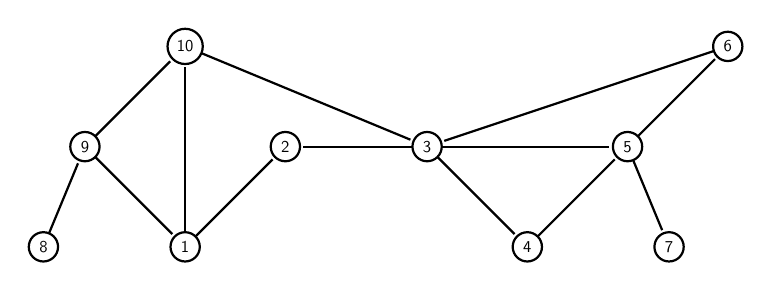
\begin{tikzpicture}[-,>=stealth,shorten >=1pt,auto,node distance=3cm,thick,main node/.style={scale=0.6,circle,draw,font=\sffamily\normalsize}]
                \node[main node] (1) {1};
                \node[main node] (2) [above right of=1]{2};
                \node[main node] (3) [right of=2]{3};
                \node[main node] (4) [below right of=3]{4};
                \node[main node] (5) [above right of=4]{5};
                \node[main node] (6) [above right of=5]{6};
                \node[main node] (7) [right of=4]{7};
                \node[main node] (8) [left of=1]{8};
                \node[main node] (9) [above left of=1]{9};
                \node[main node] (10) [above left of=2]{10};
    
                \path[every node/.style={font=\sffamily\small}]
                    (1) edge (2)
                    (3) edge (2)
                    (3) edge (5)
                    (3) edge (4)
                    (5) edge (6)
                    (5) edge (7)
                    (8) edge (9)
                    (6) edge (3)
                    (10) edge (3)
                    (9) edge (1)
                    (9) edge (10)
                    (1) edge (10)
                    (4) edge (5)
                ;
    
                \path[every node/.style={font=\sffamily\small}]
                    [color=red]
                ;
            \end{tikzpicture}
        \end{center}

        \item Eseguendo una DFS sul vertice $1$, otteniamo il seguente albero di visita $T$:
        
        \begin{center}
            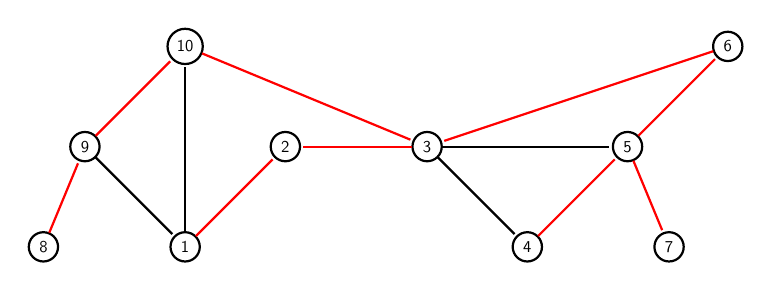
\begin{tikzpicture}[-,>=stealth,shorten >=1pt,auto,node distance=3cm,thick,main node/.style={scale=0.6,circle,draw,font=\sffamily\normalsize}]
                \node[main node] (1) {1};
                \node[main node] (2) [above right of=1]{2};
                \node[main node] (3) [right of=2]{3};
                \node[main node] (4) [below right of=3]{4};
                \node[main node] (5) [above right of=4]{5};
                \node[main node] (6) [above right of=5]{6};
                \node[main node] (7) [right of=4]{7};
                \node[main node] (8) [left of=1]{8};
                \node[main node] (9) [above left of=1]{9};
                \node[main node] (10) [above left of=2]{10};
    
                \path[every node/.style={font=\sffamily\small}]
                    (3) edge (5)
                    (1) edge (10)
                    (9) edge (1)
                    (3) edge (4)
                ;
    
                \path[every node/.style={font=\sffamily\small}]
                    [color=red]
                    (1) edge (2)
                    (3) edge (2)
                    (6) edge (3)
                    (5) edge (6)
                    (5) edge (7)
                    (9) edge (10)
                    (10) edge (3)
                    (8) edge (9)
                    (4) edge (5)
                ;
            \end{tikzpicture}
        \end{center}

        \item Dato l'arco $(3,6) \in E(T)$, il sotto-albero dei discendenti $T_6$ generato corrisponde a
        
        \begin{center}
            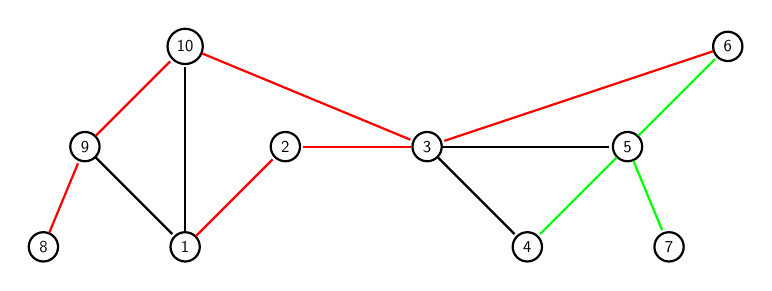
\begin{tikzpicture}[-,>=stealth,shorten >=1pt,auto,node distance=3cm,thick,main node/.style={scale=0.6,circle,draw,font=\sffamily\normalsize}]
                \node[main node] (1) {1};
                \node[main node] (2) [above right of=1]{2};
                \node[main node] (3) [right of=2]{3};
                \node[main node] (4) [below right of=3]{4};
                \node[main node] (5) [above right of=4]{5};
                \node[main node] (6) [above right of=5]{6};
                \node[main node] (7) [right of=4]{7};
                \node[main node] (8) [left of=1]{8};
                \node[main node] (9) [above left of=1]{9};
                \node[main node] (10) [above left of=2]{10};
    
                \path[every node/.style={font=\sffamily\small}]
                    (3) edge (5)
                    (1) edge (10)
                    (9) edge (1)
                    (3) edge (4)
                ;
    
                \path[every node/.style={font=\sffamily\small}]
                    [color=red]
                    (1) edge (2)
                    (3) edge (2)
                    (6) edge (3)
                    (9) edge (10)
                    (10) edge (3)
                    (8) edge (9)
                ;

                \path[every node/.style={font=\sffamily\small}]
                    [color=green]
                    (5) edge (6)
                    (5) edge (7)
                    (5) edge (4)
                ;
            \end{tikzpicture}
        \end{center}
    \end{itemize}

    \newpage
    
    \begin{framedthm}{Esistenza di un ciclo contenente un arco}
        Siano $G$ un grafo non diretto connesso, $T$ un albero di visita generato da una DFS su $G$ e $T_y$ l'albero dei discendenti di $y$ in $T$ generato da un arco $(x,y) \in E(T)$.
        
        Dati un vertice $u \in V(T_y)$ ed un vertice $v \in V(T-T_y)$, si ha che:
        \[\exists (u,v) \neq (x,y) \in E(G) \iff \exists \text{ ciclo in } G \text{ contenente } (x,y)\]
    \end{framedthm}
    
    \textit{Dimostrazione:}

    \begin{itemize}
        \item Poiché $G$ è un grafo non diretto connesso, ogni vertice in $V(G)$ verrà visitato dalla DFS, implicando che $V(T) = V(G)$. Di conseguenza, si ha che $\forall z \notin V(T_y) \implies z \in V(T-T_y)$
        \item Sia quindi $g := (x,y) \in E(T)$. Supponiamo che esista un arco $f := (u,v) \in E(G)$ tale che $u \in V(T_y)$ e $v \in V(T-T_y)$. Poiché $x \notin V(T_y) \implies x \in V(T-T_y)$ e poiché $T$ è connesso, esiste un cammino $v e_1 \ldots e_k x$ non contenente $(u,v)$ tale che $v \to x$. Inoltre, poiché $u \in V(T_y)$, ne segue automaticamente che esiste un cammino  $y h_1 \ldots h_j u$ tale che $y \to u$.
        
        Dunque, la passeggiata $v e_1 \ldots e_k x g y h_1 \ldots h_j u f v$ risulta essere un ciclo contenente $g$
        \item Viceversa, supponiamo per assurdo che non esista tale arco e che esista un ciclo contenente $g$, implicando che esista un cammino $y d_1 \ldots d_p x$ non passante per $g$ tale che $y \to x$. Poiché $y \in V(T_y)$ e $x \in V(T-T_y)$, esisterà necessariamente un arco $d_i : (a,b) \neq (x,y) \in E(G)$ all'interno del ciclo tale che $a \in V(T_y)$ e $b \in V(T-T_y)$, contraddicendo l'ipotesi iniziale.
        
        Di conseguenza, l'unica possibilità è
        \[\nexists (u,v) \neq (x,y) \in E(G) \implies \nexists \text{ ciclo in } G \text{ contenente } (x,y)\]
        da cui per contro-nominale otteniamo che
        \[\exists \text{ ciclo in } G \text{ contenente } (x,y) \implies \exists (u,v) \neq (x,y) \in E(G)\]
        $\hfill\qed$
    \end{itemize}
    
    \textbf{Esempio:}
    \begin{itemize}
        \item Riprendendo l'esempio precedente, l'arco $(5,3) \in E(G)$ dove $5 \in V(T_6)$ e $3 \in V(T) - V(T_6)$ crea un ciclo in $G$
        

        \begin{center}
            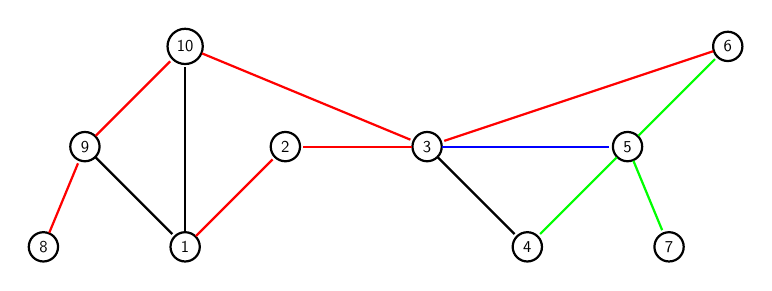
\begin{tikzpicture}[-,>=stealth,shorten >=1pt,auto,node distance=3cm,thick,main node/.style={scale=0.6,circle,draw,font=\sffamily\normalsize}]
                \node[main node] (1) {1};
                \node[main node] (2) [above right of=1]{2};
                \node[main node] (3) [right of=2]{3};
                \node[main node] (4) [below right of=3]{4};
                \node[main node] (5) [above right of=4]{5};
                \node[main node] (6) [above right of=5]{6};
                \node[main node] (7) [right of=4]{7};
                \node[main node] (8) [left of=1]{8};
                \node[main node] (9) [above left of=1]{9};
                \node[main node] (10) [above left of=2]{10};
    
                \path[every node/.style={font=\sffamily\small}]
                    (1) edge (10)
                    (9) edge (1)
                    (3) edge (4)
                ;
    
                \path[every node/.style={font=\sffamily\small}]
                    [color=red]
                    (1) edge (2)
                    (3) edge (2)
                    (6) edge (3)
                    (9) edge (10)
                    (10) edge (3)
                    (8) edge (9)
                ;

                \path[every node/.style={font=\sffamily\small}]
                    [color=green]
                    (5) edge (6)
                    (5) edge (7)
                    (5) edge (4)
                ;

                \path[every node/.style={font=\sffamily\small}]
                    [color=blue]
                    (3) edge (5)
                ;
            \end{tikzpicture}
        \end{center}
    \end{itemize}

    \begin{framedobs}{}
        Sia $G$ un grafo non diretto connesso. Dato un arco $(u,v) \in E(T)$, se $(u,v)$ è un ponte, eseguendo una DFS su $G$ radicata in $u$, si ha che $(u,v) \in E(T)$, dove $T$ è l'albero generato dalla DFS
    \end{framedobs}

    \textit{Dimostrazione:}

    \begin{itemize}
        \item Poiché $(u,v)$ è un ponte, ne segue che non esista un ciclo contenente $(u,v)$, implicando a sua volta che non esista un cammino non contenente $(u,v)$ tale che $u \to v$.
        \item Di conseguenza, poiché $G$ è connesso non diretto, dunque $V(T) = V(G)$, l'unica possibilità affinché $u,v \in V(T)$ e se $(u,v) \in E(T)$
        
        $\hfill\qed$
    \end{itemize}

    \begin{framedobs}{}
        Sia $G$ un grafo non diretto e sia $T$ un albero di visita generato da una DFS su $G$.

        Se esiste un arco $(x,y) \in E(G)-E(T)$ tale che $deg^T(x)=deg^T(y)=1$ in $T$, allora $x$ o $y$ devono essere la radice di $T$
    \end{framedobs}

    \textit{Dimostrazione:}

    \begin{itemize}
        \item Supponiamo per assurdo che né $x$ né $y$ siano la radice di $T$, dunque che $\exists (u,x), (v,y) \in E(T)$ tramite cui vengono visitati $x$ e $y$ nella DFS.
        \item Poiché $deg^T(x)=1$, ne segue che al momento della visita di $x$ il vertice $y$ fosse stato già visitato, poiché altrimenti si avrebbe che $(x,y) \in E(T)$. Analogamente, poiché $deg^T(y)=1$, ne segue che al momento della visita di $y$ il vertice $x$ fosse stato già visitato, poiché altrimenti si avrebbe che $(y,x) \in E(T) \implies (x,y) \in E(T)$.
        
        \item Di conseguenza, si ha che $Int(x) \cap Int(y) = \varnothing$, implicando che l'arco $(x,y) \in E(G)-E(T)$ sia un arco di attraversamento, contraddicendo la proposizione per cui in $G$, essendo un grafo non diretto, non possano esistere archi di attraversamento. Dunque, l'unica possibilità è che $x$ o $y$ sia necessariamente la radice del DFS
        
        $\hfill\qed$
    \end{itemize}

    \begin{framedalgo}{Trovare i ponti di un grafo (Ottim.)}
        Sia $G$ un grafo non diretto connesso rappresentato tramite liste di adiacenza. Il seguente algoritmo trova i ponti presenti in $G$.

        Il \textbf{costo} risulta essere $O(n+m)$, dove $\abs{V(G)}=n$ e $\abs{E(G)}=m$
    \end{framedalgo}

    
    \begin{algorithm}[H]
        \caption{Trovare i ponti in un grafo non diretto connesso (Ottimizzato)}\label{find_bridges_3}
        \KwIn{\\
        G: grafo non diretto connesso a liste di adiacenza,\\
        c: contatore,\\
        t: array tempi di visita,\\
        Back: array dei vertici esterni ai sotto-alberi più lontani e adiacenti ad un vertice interno ai sotto-alberi\\
        Padri: array dei padri}
        \KwOut{\\
        Insieme dei ponti presenti in $G$}
        
        \Fn{\texttt{\upshape DFS\_Bridges(G, x, c, t, Back, Padri):}}{
            \texttt{c.increment()}\;
            \texttt{t[$x$] = c}\;
            \texttt{Back[$x$] = t[$x$]}\;
            \For{$y \in V(G) \mid (x,y) \in E(G)$}{
                \uIf{\texttt{t[$y$] = 0}}{
                    \texttt{Padri[$y$] = $x$}\;
                    \texttt{DFS\_Bridges(G, y, c, t, Back, Padri)}\;
                    \uIf{\texttt{Back[$y$] < Back[$x$]}}{
                        \texttt{Back[$x$] = Back[$y$]}\;
                    }
                }
                \uElseIf{\texttt{$y \neq $ Padri[$x$]}}{
                    \uIf{\texttt{t[$y$] < Back[$x$]}}{
                        \texttt{Back[$x$] = t[$y$]}\;
                    }
                }
            }
        }

        \Fn{\texttt{\upshape findBridges\_3(G):}}{
            \texttt{$v$ = $v \in V(G)$}\;
            \texttt{\textbf{Counter} c = 0}\;
            \texttt{t, Back = [0, \ldots, 0]}\;
            \texttt{Padri = [-1, \ldots, -1]}\;
            \texttt{Padri[$v$] = $v$} \qquad\qquad //$v$ è la radice\;
            \texttt{DFS\_Bridges(G, v, c, t, Back, Padri)}\;
            \texttt{Bridges = $\varnothing$}\;
            \For{$u \in V(G)$}{
                \uIf{\texttt{Back[$u$] == t[$u$] \textbf{and} $u \neq $ Padri[$u$]}}{
                    \texttt{Bridges.add($($Padri[$u$], $u)$)}\;
                }
            }
            \texttt{return Bridges}\;
        }
    \end{algorithm}
    
    \textit{Dimostrazione correttezza e costo algoritmo:}

    \begin{itemize}
        \item Sia $x$ il vertice attualmente esplorato durante la ricorsione della funzione \texttt{DFS\_Bridges}.
        
        \item Tramite il ciclo for, proseguiamo con la ricorsione sui vertici $y \in V(G) \mid t[x]=0, (x,y) \in E(G)$, implicando che $y$ non sia già stato visitato. L'effetto ottenuto, dunque, è quello di una DFS.
        
        \item Dato l'albero $T$ generato dalla DFS, siano $y_0, \ldots, y_k$ i vertici adiacenti ad $x$ esplorati nella DFS per la prima volta tramite $x$ stesso, implicando che essi siano discendenti di $x$, dunque che $y_0, \ldots, y_k \in V(T_x)$.
        \item Siano invece $z_0, \ldots z_h$ i vertici adiacenti ad $x$ già visitati dalla DFS, implicando che $z_0, \ldots, z_j \in V(T-T_x)$, dove in particolare, per via dell'else-if, si ha che $z_i \neq p_x, \forall i \in [0,h]$, dove $p_x:=\texttt{Padri[$x$]}$
        \item Sia quindi \texttt{Back[$x$] = $t(b_x)$}, dove $b_x$ è il vertice in $V(T-T_x)$ con tempo di visita minore possibile tale che $\exists (d_x, b_x) \in E(G)$ dove $d_x \in V(T_x)$, implicando che:
        \[\texttt{Back[$x$]} = \min(\texttt{Back[$y_0$], $\ldots$, Back[$y_k$], t[$y$], t[$z_0$], \ldots, t[$z_h$]})\]
        \item Nel caso in cui \texttt{Back[$x$] $\neq$ t[$x$]}, dunque $b_x \neq x$, esisterebbe un arco $(b_x, d_x) \neq (p_x, x) \in E(G)$ tale che $b_x \in V(T-T_x)$ e $d_x \in V(T_x)$. Per il teorema precedente, tale arco può esistere se e solo se esiste un ciclo in $G$ contenente l'arco $(p_x, x) \in E(G)$. Di conseguenza, si ha che $(p_x, x)$ è un ponte se e solo se \texttt{Back[$x$] $=$ t[$x$]}.
        \item Poiché l'algoritmo effettua una DFS ricorsiva modificata e il costo di tutte le operazioni della ricorsione è $O(1)$, il costo computazionale totale risulta essere $O(n+m)$
        
        $\hfill\qed$
    \end{itemize}

    \quad

    \section{Componenti di un grafo}

    \quad

    \begin{framedprop}{}
        Sia $G$ un grafo diretto. Dato un vertice $x \in V(G)$, si ha che:
        \[G \text{ fortemente connesso } \iff \forall y \in V(G), \exists \text{ due cammini } \mid  x \to y, y \to x\]
    \end{framedprop}

    \begin{itemize}
        \item Se $G$ è fortemente connesso, per definizione stessa ne segue automaticamente che $ \forall y \in V(G), \exists \text{ due cammini } \mid  x \to y, y \to x$
        \item Viceversa, se $\forall y \in V(G), \exists \text{ due cammini } \mid  x \to y, y \to x$, per ogni coppia di vertici $u,v \in V(G)$ si ha che $u \to x \to v$ e $v \to x \to u$, dunque $G$ è fortemente connesso
        
        $\hfill\qed$
    \end{itemize}

    \begin{framedobs}{}
        Sia $G$ un grafo. Se $\abs{V(G)} =1$, allora $G$ è fortemente connesso, poiché l'unico vertice $v \in V(G)$ può raggiungere se stesso tramite il cammino nullo
    \end{framedobs}


    \begin{frameddefn}{Componenti di un grafo}
        Sia $G$ un grafo. Definiamo come \textbf{componente} di $G$ un sotto-grafo $H \subseteq G$ \textbf{fortemente connesso e massimale}, ossia $\nexists H' \subseteq G \mid H \subset H'$ fortemente connesso.

        Dato un vertice $v \in V(G)$, indichiamo come $comp(v)$ il componente $comp(v) \subseteq G$ tale che $v \in comp(v)$
    \end{frameddefn}

    \textbf{Esempio:}

    \begin{itemize}
        \item I componenti del seguente grafo corrispondono a $H_1 := \{ 1,2,3,5,6\}, H_2 := \{ 4\}, H_3 := \{7\}$
        \begin{center}
            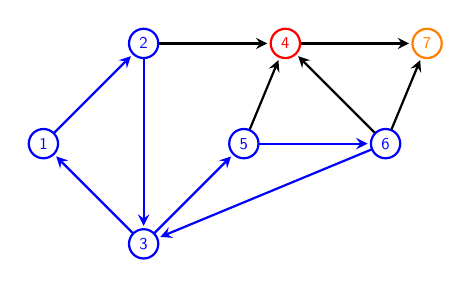
\begin{tikzpicture}[->,>=stealth,shorten >=1pt,auto,node distance=3cm,thick,main node/.style={scale=0.6,circle,draw,font=\sffamily\normalsize}]
                \node[main node] (1) [color=blue]{1};
                \node[main node] (2) [color=blue, above right of=1]{2};
                \node[main node] (3) [color=blue, below right of=1]{3};
                \node[main node] (4) [color=red, right of=2]{4};
                \node[main node] (5) [color=blue, above right of=3]{5};
                \node[main node] (6) [color=blue, right of=5]{6};
                \node[main node] (7) [color=orange, right of=4]{7};

                \path[every node/.style={font=\sffamily\small}]
                    (5) edge (4)
                    (2) edge (4)
                    (4) edge (7)
                    (6) edge (7)
                    (6) edge (4)
                ;

                \path[every node/.style={font=\sffamily\small}]
                    [color=blue]
                    (1) edge (2)
                    (2) edge (3)
                    (3) edge (1)
                    (3) edge (5)
                    (5) edge (6)
                    (6) edge (3)
                ;
            \end{tikzpicture}
        \end{center}
    \end{itemize}
    
    \begin{framedobs}{}
        Sia $G$ un grafo. Date le sue componenti $H_1, \ldots, H_k \subseteq G$, si ha che
        \[H_i \cap H_j = \varnothing, \forall i \neq j\]
    \end{framedobs}

    \textit{Dimostrazione:}

    \begin{itemize}
        \item Date le componenti $H_1, \ldots, H_k$ diverse tra loro, supponiamo per assurdo che $\exists i,j \in [1,k] \mid H_i \cap H_j \neq \varnothing$, implicando che $\exists v \in V(H_i) \cap V(H_j) \iff v \in V(H_i), v \in v(H_j)$.
        \item Poiché $H_i$ è fortemente connesso, si ha che $\forall x \in H_i$ esistono due cammini tali che $v \to x, x \to v$. Analogamente, $\forall y \in H_j$ esistono due cammini tali che $v \to y, y \to v$. Di conseguenza, si avrebbe che $\forall x \in H_i, \forall y \in H_j$ esistono due cammini tali che $x \to v \to y$ e $y \to v \to x$, implicando che $H_i = H_j$ e contraddicendo l'ipotesi
        
        $\hfill\qed$
    \end{itemize}

    \begin{frameddefn}{Contrazione in un vertice}
        Sia $G$ un grafo. Dato un sotto-grafo fortemente connesso $H \subseteq G$, definiamo come \textbf{contrazione di $H$ in un vertice $v_H$} l'operazione tramite cui:
        \begin{itemize}
            \item Vengono rimossi da $V(G)$ i vertici in $V(H)$, sostituendoli con un vertice $v_H$
            \item Vengono rimossi tutti gli archi $(u,v), (v',u') \in E(G)$ tali che $u,u' \in V(H)$ e $v,v' \in V(G)-V(H)$, sostituendoli con un arco $(v_H, v)$ e un arco $(v', v_H)$
        \end{itemize}

        Il grafo ottenuto viene indicato come $G/V(H)$, letto "$G$ \textbf{contratto} $V(H)$"
    \end{frameddefn}

    \newpage

    \textbf{Esempio:}

    \begin{itemize}
        \item Consideriamo ancora il grafo precedente. 

        \begin{center}
            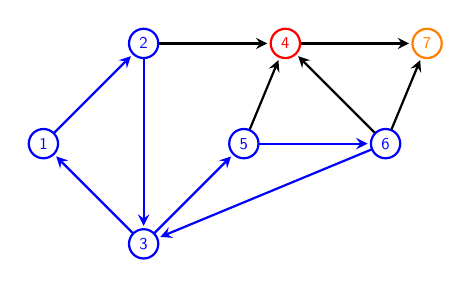
\begin{tikzpicture}[->,>=stealth,shorten >=1pt,auto,node distance=3cm,thick,main node/.style={scale=0.6,circle,draw,font=\sffamily\normalsize}]
                \node[main node] (1) [color=blue]{1};
                \node[main node] (2) [color=blue, above right of=1]{2};
                \node[main node] (3) [color=blue, below right of=1]{3};
                \node[main node] (4) [color=red, right of=2]{4};
                \node[main node] (5) [color=blue, above right of=3]{5};
                \node[main node] (6) [color=blue, right of=5]{6};
                \node[main node] (7) [color=orange, right of=4]{7};

                \path[every node/.style={font=\sffamily\small}]
                    (5) edge (4)
                    (2) edge (4)
                    (4) edge (7)
                    (6) edge (7)
                    (6) edge (4)
                ;

                \path[every node/.style={font=\sffamily\small}]
                    [color=blue]
                    (1) edge (2)
                    (2) edge (3)
                    (3) edge (1)
                    (3) edge (5)
                    (5) edge (6)
                    (6) edge (3)
                ;
            \end{tikzpicture}
        \end{center}

        \item Poiché il componente $H_1 := \{ 1,2,3,5,6\}$ è un grafo fortemente connesso, possiamo contrarre $H_1$ nel vertice $v_{H_1}$. Il grafo $G/V(H_1)$ risultante corrisponde a:
        
        \begin{center}
            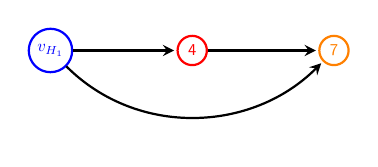
\begin{tikzpicture}[->,>=stealth,shorten >=1pt,auto,node distance=3cm,thick,main node/.style={scale=0.6,circle,draw,font=\sffamily\normalsize}]
                \node[main node] (vH1) [color=blue]{$v_{H_1}$};
                \node[main node] (4) [color=red, right of=vH1]{4};
                \node[main node] (7) [color=orange, right of=4]{7};

                \path[every node/.style={font=\sffamily\small}]
                    (vH1) edge (4)
                    (4) edge (7)
                    (vH1) edge [out=-45, in=225] (7)
                ;

            \end{tikzpicture}
        \end{center}
    \end{itemize}

    \begin{framedthm}{Contrazione di un sotto-grafo fortemente connesso}
        Sia $G$ un grafo \textbf{fortemente connesso}. Dato un \textbf{sotto-grafo fortemente connesso} $H \subseteq G$, allora $G/V(H)$ è \textbf{fortemente connesso}
    \end{framedthm}

    \textit{Dimostrazione:}

    \begin{itemize}
        \item Dato $u \neq v_H \in V(G/V(H))$, si ha che $u \in V(G)$. Poiché $G$ è fortemente connesso, esistono due cammini tali che $u \to h$ e $h \to u$ in $G$, dove $h \in V(H)$.
        
        \item Sia quindi $v_{H} \in G/V(H)$ il vertice in cui è stato contratto $H$. Poiché $u \to h$ in $G$, ne segue che esista un cammino $u \to v_H$ in $G/V(H)$. Analogamente, poiché $h \to u$ in $G$, ne segue che esista un cammino $v_H \to u$ in $G/V(H)$. Dunque, concludiamo che $G/V(H)$ sia fortemente connesso.
        
        $\hfill\qed$
    \end{itemize}

    \begin{framedlem}{}
        Un \textbf{grafo fortemente connesso diretto} $G$ dove $\abs{V(G)} > 1$ è sempre \textbf{ciclico}
    \end{framedlem}

    \textit{Dimostrazione:}
    \begin{itemize}
        \item Dati $u,v \in V(G)$, poiché $G$ è fortemente connesso si ha che esiste un cammino diretto $ue_1\ldots e_k v$ tale che $u \to v$ ed un cammino diretto $vh_1\ldots h_j u$ tale che $v \to u$.
        \item Di conseguenza, esiste sempre un ciclo $ue_1\ldots e_k vh_1\ldots h_j u$
        
        $\hfill\qed$
    \end{itemize}

    \begin{framedlem}{}
        Sia $G$ un grafo. Dato un ciclo $v_0e_1v_1\ldots v_{k-1}e_{k-1}v_ke_kv_0$ in $G$, il sotto-grafo $C \subseteq G$ tale che $v_0, v_1, \ldots, v_{k-1},v_k \in V(C)$ e $e_1,\ldots, e_k \in E(C)$ è un grafo \textbf{fortemente connesso}
    \end{framedlem}

    \textit{Dimostrazione:}

    \begin{itemize}
        \item Sia $C \subseteq G$ tale che $v_0, v_1, \ldots, v_{k-1},v_k \in V(C)$ e $e_1,\ldots, e_k \in E(C)$
        \item Essendo $v_0e_1v_1\ldots v_{k-1}e_{k-1}v_ke_kv_0$ un ciclo in $G$, tale ciclo risulta esistere anche in $C$, dunque si ha che $\forall v_i, v_j \in V(C) \mid i \neq j \implies v_i \to v_j, v_j \to v_i$ in $C$
        
        $\hfill\qed$
    \end{itemize}
    
    \begin{framedalgo}{Trovare i componenti di un grafo diretto}
        Sia $G$ un grafo diretto rappresentato tramite liste di adiacenza. Il seguente algoritmo trova i componenti di $G$.

        Il \textbf{costo} risulta essere $O(n(n+m))$, dove $\abs{V(G)}=n$ e $\abs{E(G)}=m$
    \end{framedalgo}

    
    \begin{algorithm}[H]
        \caption{Trovare i componenti di un grafo diretto}\label{components_1}
        \KwIn{\\
        G: grafo a liste di adiacenza}
        \KwOut{\\
        Insieme di componenti in $G$}
        
        \Fn{\texttt{\upshape getComponents(G):}}{
            \texttt{$C$ = findCycle(G)}\;
            \eIf{$C == \varnothing$}{
                \texttt{return $\{\{v\} \mid  v \in V(G)\}$} \qquad\qquad //è un insieme di insiemi\;
            }
            {
                \texttt{$G/V(C)$, $v_C$ = contractGraph($G$, $C$)}\;
                \texttt{$\{H_1, \ldots, H_k\}$ = getComponents($G/V(C)$)}\;
                \texttt{uncontrComponents = $\varnothing$}\;
                \For{$i = 1, \ldots, k$}{
                    \eIf{$v_C \notin H_i$}{
                        \texttt{uncontrComponents.add($H_i$)}\;
                    }
                    {
                        \texttt{$H_i'$ = $(H_i - \{v_C\}) \cup V(C)$}\;
                        \texttt{uncontrComponents.add($H_i'$)}\;
                    }
                }
            }
            \texttt{return uncontrComponents}\;
        }
    \end{algorithm}

    \newpage

    \textit{Dimostrazione correttezza algoritmo:}

    \begin{itemize}
        \item Sia $H$ un componente di $G$. Se $\abs{V(H)} > 1$, per dimostrazione precedente esiste un ciclo in $H$ poiché $H$ è un sotto-grafo diretto fortemente connesso.
        \item Sia quindi $C$ il sotto-grafo composto dagli archi e i vertici di tale ciclo, implicando che, per il lemma precedente, $C$ sia fortemente connesso. Per il teorema precedente, dunque, anche $H' := H/V(C)$ risulta essere fortemente connesso, implicando che esso sia un componente di $G/V(C)$.
        \item Applicando tale procedimento ricorsivamente, l'intero componente $H$ arriverà ad essere contratto in un singolo vertice $v_H$, il quale risulterà essere un componente connesso della versione finale del grafo $G_f$.
        \item Una volta raggiunto il caso base, ossia una volta che $C == \varnothing$, ogni punto del grafo $G_f$ sarà un componente di quest'ultimo, implicando che i vertici $v_{H_1}, \ldots, v_{H_k} \in V(G_f)$ siano le contrazioni massime dei componenti $comp(v_{H_1}), \ldots, comp(v_{H_k})$ di $G$.
        \item Sia quindi $H_i = comp(v_{H_i})$ e siano $H_i/V(C_0), \ldots, H_i/V(C_q)$ le contrazioni interne ad $H_i$ tramite i cicli $C_0, \ldots, C_q$ generati dalla ricorsione ad ogni contrazione.
        \item Durante la risalita della ricorsione, ogni contrazione viene invertita, sostituendo nella contrazione $H_i/V(C_j)$ il vertice $v_{C_{j-1}}$ con i vertici originali $V(C_{j-1})$. Una volta terminata la risalita, dunque, si avrà che $H_i \in \texttt{uncontrComponents}$
        \item L'insieme finale restitutito dalla prima chiamata della ricorsione, dunque, corrisponderà a $\{comp(v_{H_1}), \ldots, comp(v_{H_k})\}$ 

        $\hfill\qed$
    \end{itemize}

    \textit{Dimostrazione costo algoritmo:}

    \begin{itemize}
        \item Il costo dell'algoritmo \ref{findCycle_2} \texttt{findCycle()} proposto in precedenza è pari a $O(n+m)$
        \item Consideriamo quindi la contrazione del grafo $G$ tramite la funzione \texttt{contractGraph()}. Per poter eliminare tutti i vertici in $V(C)$ e gli archi in $E(C)$, sostituendo quest'ultimi con gli archi connessi a $v_c$, nel caso peggiore è necessario scorrere tutte le liste di adiacenza di tutti i vertici, rendendo il costo di tale operazaione pari a $O(n+m)$
        \item Per quanto riguarda il ciclo for, invece, nel caso peggiore in cui ogni vertice di $G$ sia un componente, si ha che $k = \abs{V(G) = n}$. Inoltre, poiché ogni operazione all'interno del ciclo ha un costo $O(1)$, il costo dell'intero ciclo risulta essere $O(n)$
        \item Dunque, concludiamo che il costo di una singola chiamata ricorsiva sia $O(n+m)+O(n+m)+O(n) = O(n+m)$. Infine, poiché ad ogni ricorsione viene contratto un sotto-grafo di $G$, ne segue che vi possano essere massimo $n$ chiamate ricorsive, rendendo il costo totale dell'algoritmo pari a $O(n(n+m))$
        
        $\hfill\qed$
    \end{itemize}

    \newpage
    
    \textbf{Esempio:}

    \begin{itemize}
        \item Consideriamo il seguente grafo su cui applicheremo l'algoritmo precedente
        \begin{center}
            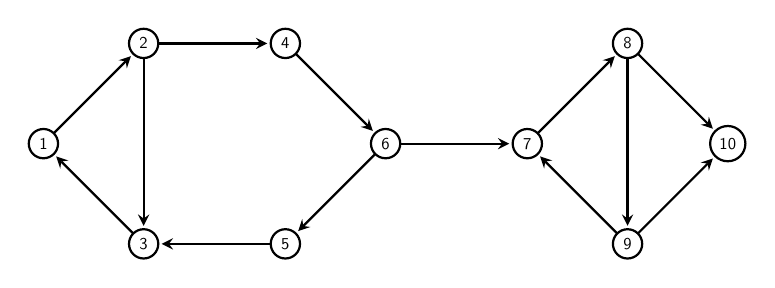
\begin{tikzpicture}[->,>=stealth,shorten >=1pt,auto,node distance=3cm,thick,main node/.style={scale=0.6,circle,draw,font=\sffamily\normalsize}]
                \node[main node] (1) {1};
                \node[main node] (2) [above right of=1]{2};
                \node[main node] (3) [below right of=1]{3};
                \node[main node] (4) [right of=2]{4};
                \node[main node] (5) [right of=3]{5};
                \node[main node] (6) [below right of=4]{6};
                \node[main node] (7) [right of=6]{7};
                \node[main node] (8) [above right of=7]{8};
                \node[main node] (9) [below right of=7]{9};
                \node[main node] (10) [below right of=8]{10};

                \path[every node/.style={font=\sffamily\small}]
                    (1) edge (2)
                    (3) edge (1)
                    (2) edge (4)
                    (5) edge (3)
                    (2) edge (3)
                    (4) edge (6)
                    (6) edge (5)
                    (6) edge (7)
                    (7) edge (8)
                    (8) edge (9)
                    (9) edge (7)
                    (8) edge (10)
                    (9) edge (10)
                ;

            \end{tikzpicture}
        \end{center}

        \item Alla prima chiamata ricorsiva, viene trovato il ciclo $C_1 := \{1,2,3\}$, il quale viene contrarro nel vertice $v_{C_1}$
        
        \begin{center}
            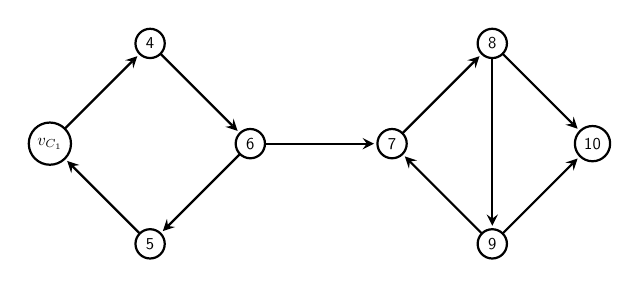
\begin{tikzpicture}[->,>=stealth,shorten >=1pt,auto,node distance=3cm,thick,main node/.style={scale=0.6,circle,draw,font=\sffamily\normalsize}]
                \node[main node] (vC1) {$v_{C_1}$};
                \node[main node] (4) [above right of=vC1]{4};
                \node[main node] (5) [below right of=vC1]{5};
                \node[main node] (6) [below right of=4]{6};
                \node[main node] (7) [right of=6]{7};
                \node[main node] (8) [above right of=7]{8};
                \node[main node] (9) [below right of=7]{9};
                \node[main node] (10) [below right of=8]{10};

                \path[every node/.style={font=\sffamily\small}]
                    (vC1) edge (4)
                    (5) edge (vC1)
                    (4) edge (6)
                    (6) edge (5)
                    (6) edge (7)
                    (7) edge (8)
                    (8) edge (9)
                    (9) edge (7)
                    (8) edge (10)
                    (9) edge (10)
                ;

            \end{tikzpicture}
        \end{center}

        \item Alla seconda chiamata ricorsiva, viene trovato il ciclo $C_2 := \{7,8,9\}$, il quale viene contratto nel vertice $v_{C_2}$
        
        \begin{center}
            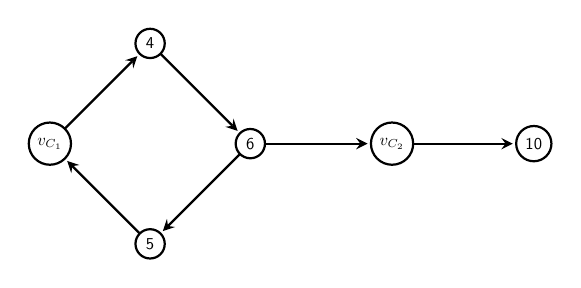
\begin{tikzpicture}[->,>=stealth,shorten >=1pt,auto,node distance=3cm,thick,main node/.style={scale=0.6,circle,draw,font=\sffamily\normalsize}]
                \node[main node] (vC1) {$v_{C_1}$};
                \node[main node] (4) [above right of=vC1]{4};
                \node[main node] (5) [below right of=vC1]{5};
                \node[main node] (6) [below right of=4]{6};
                \node[main node] (vC2) [right of=6]{$v_{C_2}$};
                \node[main node] (10) [right of=vC2]{10};

                \path[every node/.style={font=\sffamily\small}]
                    (vC1) edge (4)
                    (5) edge (vC1)
                    (4) edge (6)
                    (6) edge (5)
                    (6) edge (vC2)
                    (vC2) edge (10)
                ;

            \end{tikzpicture}
        \end{center}

        \item Alla terza chiamata ricorsiva, viene trovato il ciclo $C_3 := \{v_{C_1}, 4,5,6\}$, il quale viene contratto nel vertice $v_{C_3}$
        
        \begin{center}
            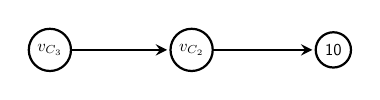
\begin{tikzpicture}[->,>=stealth,shorten >=1pt,auto,node distance=3cm,thick,main node/.style={scale=0.6,circle,draw,font=\sffamily\normalsize}]
                \node[main node] (vC3) {$v_{C_3}$};
                \node[main node] (vC2) [right of=vC3]{$v_{C_2}$};
                \node[main node] (10) [right of=vC2]{10};

                \path[every node/.style={font=\sffamily\small}]
                    (vC3) edge (vC2)
                    (vC2) edge (10)
                ;

            \end{tikzpicture}
        \end{center}

        \item A questo punto, raggiunto il caso base, i vertici rimanenti risultano essere le contrazioni massime dei componenti di $G$. Durante la risalita della ricorsione, de-contraendo tali componenti otteniamo che:
        
        \begin{center}
            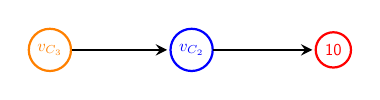
\begin{tikzpicture}[->,>=stealth,shorten >=1pt,auto,node distance=3cm,thick,main node/.style={scale=0.6,circle,draw,font=\sffamily\normalsize}]
                \node[main node] (vC3) [color=orange]{$v_{C_3}$};
                \node[main node] (vC2) [color=blue, right of=vC3]{$v_{C_2}$};
                \node[main node] (10) [color=red, right of=vC2]{10};

                \path[every node/.style={font=\sffamily\small}]
                    (vC3) edge (vC2)
                    (vC2) edge (10)
                ;

            \end{tikzpicture}
        \end{center}
    \end{itemize}
        
    \quad

    \begin{center}

        \begin{tabular}{c c c c}
            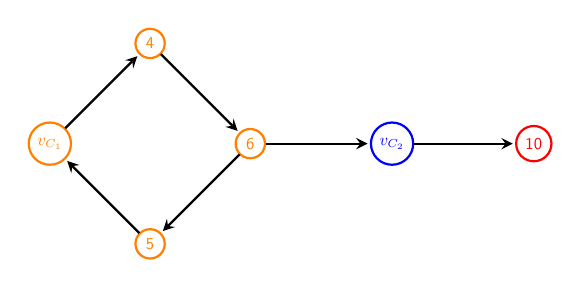
\begin{tikzpicture}[->,>=stealth,shorten >=1pt,auto,node distance=3cm,thick,main node/.style={scale=0.6,circle,draw,font=\sffamily\normalsize}]
                \node[main node] (vC1) [color=orange]{$v_{C_1}$};
                \node[main node] (4) [color=orange, above right of=vC1]{4};
                \node[main node] (5) [color=orange, below right of=vC1]{5};
                \node[main node] (6) [color=orange, below right of=4]{6};
                \node[main node] (vC2) [color=blue, right of=6]{$v_{C_2}$};
                \node[main node] (10) [color=red, right of=vC2]{10};

                \path[every node/.style={font=\sffamily\small}]
                    (vC1) edge (4)
                    (5) edge (vC1)
                    (4) edge (6)
                    (6) edge (5)
                    (6) edge (vC2)
                    (vC2) edge (10)
                ;
            \end{tikzpicture}

            &\qquad&

            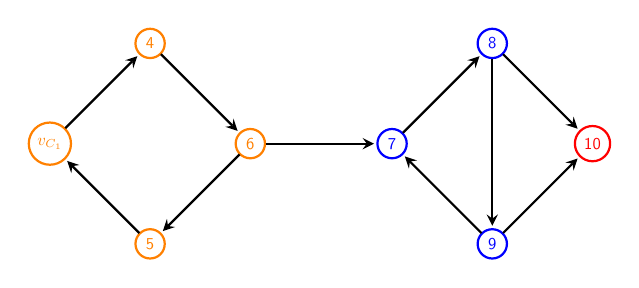
\begin{tikzpicture}[->,>=stealth,shorten >=1pt,auto,node distance=3cm,thick,main node/.style={scale=0.6,circle,draw,font=\sffamily\normalsize}]
                \node[main node] (vC1) [color=orange]{$v_{C_1}$};
                \node[main node] (4) [color=orange, above right of=vC1]{4};
                \node[main node] (5) [color=orange, below right of=vC1]{5};
                \node[main node] (6) [color=orange, below right of=4]{6};
                \node[main node] (7) [color=blue,right of=6]{7};
                \node[main node] (8) [color=blue, above right of=7]{8};
                \node[main node] (9) [color=blue, below right of=7]{9};
                \node[main node] (10) [color=red, below right of=8]{10};

                \path[every node/.style={font=\sffamily\small}]
                    (vC1) edge (4)
                    (5) edge (vC1)
                    (4) edge (6)
                    (6) edge (5)
                    (6) edge (7)
                    (7) edge (8)
                    (8) edge (9)
                    (9) edge (7)
                    (8) edge (10)
                    (9) edge (10)
                ;

            \end{tikzpicture}
        \end{tabular}
    \end{center}
    

    \quad

    \begin{center}
        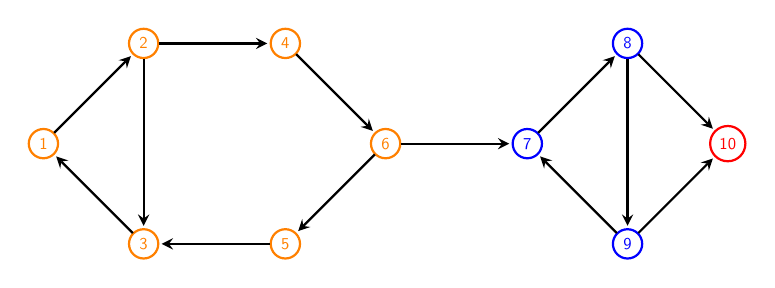
\begin{tikzpicture}[->,>=stealth,shorten >=1pt,auto,node distance=3cm,thick,main node/.style={scale=0.6,circle,draw,font=\sffamily\normalsize}]
            \node[main node] (1) [color=orange]{1};
            \node[main node] (2) [color=orange, above right of=1]{2};
            \node[main node] (3) [color=orange, below right of=1]{3};
            \node[main node] (4) [color=orange, right of=2]{4};
            \node[main node] (5) [color=orange, right of=3]{5};
            \node[main node] (6) [color=orange, below right of=4]{6};
            \node[main node] (7) [color=blue,right of=6]{7};
            \node[main node] (8) [color=blue, above right of=7]{8};
            \node[main node] (9) [color=blue, below right of=7]{9};
            \node[main node] (10) [color=red, below right of=8]{10};
            \path[every node/.style={font=\sffamily\small}]
                (1) edge (2)
                (3) edge (1)
                (2) edge (4)
                (5) edge (3)
                (2) edge (3)
                (4) edge (6)
                (6) edge (5)
                (6) edge (7)
                (7) edge (8)
                (8) edge (9)
                (9) edge (7)
                (8) edge (10)
                (9) edge (10)
            ;

        \end{tikzpicture}
    \end{center}

    \begin{itemize}
        \item Dunque, l'output dell'algoritmo sarà $\{\{1,2,3,4,5,6\}, \{7,8,9\},\{10\}\}$
    \end{itemize}

    \quad

    \subsection{Algoritmo di Tarjan}

    \quad

    \begin{frameddefn}{C-Radice di un componente}
        Sia $G$ un grafo e sia $A$ un albero o un'arborescenza di visita generata da una DFS su $G$. Dato un vertice $v \in V(G)$, definiamo come \textbf{c-radice di $comp(v)$ in $A$} il vertice $u \in comp(v)$ visitato per primo dalla DFS 
    \end{frameddefn}

    \begin{framedprop}{}
        Sia $G$ un grafo diretto e sia $A$ un'arborescenza di visita generata da una DFS su $G$. Dato $u \in V(G)$, se $u$ è la c-radice di $comp(u)$ si ha che:
        \begin{enumerate}
            \item $V(comp(u)) \subseteq V(A_u)$, dove $A_u$ è l'arborescenza dei discendenti di $u$ in $A$
            \item $V(A_u) = V(comp(u)) \cup V(comp(u_1)) \ldots V(comp(u_k))$, dove $u_1,\ldots, u_k$ sono le c-radici in $G$ tali che $u_1, \ldots, u_k \in V(A_u)$ 
        \end{enumerate}
    \end{framedprop}

    \textit{Dimostrazioni:}

    \begin{enumerate}
        \item
        \begin{itemize}
            \item Per definizione stessa, si ha che $\forall v \in V(comp(u))$ esistono due cammini tali che $u \to v$ e $v \to u$. Di conseguenza, poiché $u \in V(A)$, ne segue necessariamente che $v$ sia raggiungibile dalla DFS, dunque che $v \in V(A)$.
            \item Inoltre, poiché $u$ è la c-radice di $comp(u)$, ne segue che $t(u) < t(v)$. Nel caso assurdo in cui $t(u) \leq T(u) < t(v) \leq T(v)$, la DFS avrebbe sbagliato a non visitare $v$ prima di rimuovere $u$ dallo stack, poiché, essendo $u$ c-radice, ogni vertice in $V(comp(u))$ non è stato ancora visitato. Di conseguenza, l'unica possibilità è che $t(u) < t(v) \leq T(v) \leq T(u)$
            \item Dunque, poiché $Int(v) \subseteq Int(u)$ e $v \in V(A)$, ne segue che $v$ sia un discendente di $u$ in $A$, implicando quindi che $V(comp(u)) \subseteq  V(A_u)$
        \end{itemize}
        \item
        \begin{itemize}
            \item Dati $u_1, \ldots, u_k \in V(A_u)$, si ha che $A_{u_1}, \ldots, A_{u_k} \subseteq A_u$. Inoltre, poiché $u_1, \ldots, u_k$ sono rispettivamente c-radici di $comp(u_1),\ldots,comp(u_k)$, per la proposizione appena dimostrata si ha che
            \[V(comp(u_i)) \subseteq V(A_{u_i}) \subseteq V(A_u), \forall i \in [1,k]\]
            \item Analogamente, per lo stesso motivo si ha che $V(comp(u)) \subseteq V(A_u)$. Di conseguenza, otteniamo che:
            \[V(comp(u)) \cup V(comp(u_1)) \ldots V(comp(u_k)) \subseteq V(A_u)\]
            
            \item Viceversa, consideriamo $w \in V(A_u)$, implicando che esiste un cammino in $A_u \subseteq A \subseteq G$, tale che $u \to w$. Supponiamo che in $G$ esista anche un cammino tale che $w \to u$. In tal caso, si avrebbe che $w \in V(comp(u))$.
            \item Supponiamo quindi che non esista tale cammino $w \to u$ in $G$. Poiché esiste un cammino $u \to w$ in $A$, ne segue che $\forall y \in V(comp(w))$ esiste un cammino tale che $u \to w \to y$, implicando che ogni vertice in $comp(w)$ possa essere raggiunto dalla DFS, dunque che $y \in V(A)$.

            \item Sia quindi $z \in V(comp(w))$ la c-radice di $comp(z) = comp(w)$. Supponiamo per assurdo che $z \in V(comp(w))\cap V(A)$ ma che $z \notin V(A_u)$, implicando necessariamente che $t(z) < t(u)$, poiché altrimenti, dato che $u \to w \to z$, si avrebbe che $z \in V(A_u)$
            
            \item Poiché $w \in V(A_u)$, ne segue che $t(z) < t(u) < t(w) \leq T(w) \leq T(u)$, per cui si ha che:
            \begin{itemize}
                \item Nel caso in cui $t(z) \leq T(z) < t(u) < t(w) \leq T(w) \leq T(u)$, la DFS avrebbe sbagliato a non visitare $w$ prima che $z$ venisse rimosso dallo stack, poiché $z \in comp(z)=comp(w) \implies z \to w$.
                \item Nel caso in cui $t(z) < t(u) < t(w) \leq T(w) \leq T(u) \leq T(z)$, si avrebbe che $A_u \subseteq A_{z}$, dunque che esiste un cammino tale che $z \to u$. Tuttavia, poiché esiste anche un cammino tale che $u \to w \to z$, otterremmo che $u \in comp(u) = comp(z)$, contraddicendo l'ipotesi per cui $u$ sia la c-radice di $comp(u)$
            \end{itemize}
            Dunque, poiché ognuno dei due casi ipotetici crea una contraddizione, concludiamo che l'unica possibilità sia che $z \in V(A_u)$

            \item Di conseguenza, poiché $z$ è una c-radice e $z \in V(A_u)$, per definizione stessa di $u_1, \ldots, u_k$ ne segue che $z \in \{u_1, \ldots, u_k\}$, da cui traiamo che:
            \[w \in V(A_u) \implies w \in comp(w) = comp(z) = comp(u_i), \exists i \in [1,k] \mid z = u_i\]

            \item Infine, poiché $w \in V(comp(u))$ oppure $\exists i \in [1,k] \mid w \in V(comp(u_i))$, concludiamo che
            \[V(A_u) \subseteq V(comp(u)) \cup V(comp(u_1)) \ldots V(comp(u_k))\]
            $\hfill\qed$
        \end{itemize}
    \end{enumerate}
    
    \begin{framedalgo}{Algoritmo di Tarjan}
        Sia $G$ un grafo diretto rappresentato tramite liste di adiacenza. Il seguente algoritmo trova i componenti di $G$.
        
        Il \textbf{costo} risulta essere $O(n+m)$, dove $\abs{V(G)}=n$ e $\abs{E(G)}=m$
    \end{framedalgo}

    \begin{algorithm}[H]
        \caption{Trovare i componenti di un grafo diretto (Algoritmo di Tarjan)}\label{components_2}
        \KwIn{\\
        G: grafo diretto a liste di adiacenza, Comp: array multiuso (\underline{leggi dimostrazione})\\
        c: Counter tempi di visita,  cc: Counter ID componente\\
        }
        \KwOut{\\
        Array dei componenti in $G$}
        
        \Fn{\texttt{\upshape DFS\_SCC(G, u, S, c, cc):}}{
            \texttt{$c$.increment()}\;
            \texttt{Comp[$u$] = $-c$}\;
            \texttt{S.push($u$)}\;
            \texttt{back = $c$}\;
            \For{$v \in u$.uscenti}{
                \uIf{\texttt{Comp[$v$] = $0$}}{
                    \texttt{back$_v$ = DFS\_SCC(G, v, Comp, S, c, cc)}\;
                    \texttt{back = min(back, back$_v$)}\;
                    
                }
                \uElseIf{\texttt{Comp[$v$] < $0$}}{
                    \texttt{back = min(back, -Comp[$v$])}\;
                }
            }
            \uIf{\texttt{back == -Comp[$u$]}}{
                \texttt{$cc$.increment()}\;
                \texttt{$w$ = S.pop()}\;
                \texttt{Comp[$w$] = $cc$}\;
                \While{$w \neq u$}{
                    \texttt{$w$ = S.pop()}\;
                    \texttt{Comp[$w$] = $cc$}\;
                }
            }
            \texttt{return back}\;
        }

        \Fn{\texttt{\upshape getComponents\_2(G):}}{
            \texttt{Comp = [0, ..., 0]}\;
            \texttt{\textbf{Counter} c, cc = 0}\;
            \texttt{\textbf{Stack} S = $\varnothing$}\;
            \For{ \texttt{$u \in V(G)$}}{
                \uIf{\texttt{Comp[$u$] = 0}}{
                    \texttt{DFS\_SCC(G, u, Comp, S, c, cc)}\;
                }
            }
            \texttt{return Comp}\;
        }
    \end{algorithm}

    \textit{Dimostrazione correttezza e costo algoritmo:}

    \begin{itemize}
        \item Siano $r_1, \ldots, r_p \in V(G)$ i vertici non ancora visitati su cui viene chiamata non ricorsivamente la funzione \texttt{DFS\_SCC}. Per la proposizione precedente, sappiamo che $V(A_{r_1} \cup \ldots \cup A_{r_{p}})$ conterranno necessariamente i vertici di tutti componenti di $G$. 
        \item Sia quindi \texttt{Comp[]} un array tale che:
        \begin{itemize}
            \item Se $x \in V(G)$ non è mai stato visitato, allora \texttt{Comp[$x$] = 0}
            \item Se $x \in V(G)$ viene visitato per la prima volta, allora \texttt{Comp[$x$] = $-t(x)$}, dove $t(x)$ è il tempo di visita di $x$ (corrispondente al valore del contatore $c$ al momento della visita di $x$)
            \item Se il componente di $x \in V(G)$ è stato già completamente determinato, allora \texttt{Comp[$x$] = cc$_{comp(x)}$}, dove \texttt{cc$_{comp(x)}$} è il valore del contatore $cc$ nel momento in cui viene determinato $comp(x)$
        \end{itemize}

        \item Notiamo inoltre che lo stack \texttt{S} contiene tutti i vertici $y \in V(G)$ per cui ancora non è stato determinato $comp(y)$.

        \item Sia $u \in V(G)$ il vertice attualmente visitato dalla DFS. Dati i vertici $v_1, \ldots, v_k \in V(G)$ tali che $(u, v_i) \in E(G), \forall i \in [1,k]$, si ha che:
        \begin{itemize}
            \item Se \texttt{Comp[$v_i$] = 0}, ne segue che $v_i \in V(A_u)$, dunque che $v_i$ sia discendente di $u$
            \item Se \texttt{Comp[$v_i$] < 0}, ne segue che $v_i$ sia un vertice già visitato ma per cui non è ancora terminata la ricorsione, implicando che $u \in V(A_{v_i})$, dunque che $v_i$ sia un antenato di $u$
            \item Se \texttt{Comp[$v_i$] > 0}, ne segue che \texttt{Comp[$v_i$] = cc$_{comp(v_i)}$}, implicando che $u \notin V(comp(v_i))$, venendo quindi direttamente saltato
        \end{itemize}
        dove $A$ è l'arborescenza di visita generata dalla DFS

        \item Siano quindi $w_1,\ldots, w_j \in V(G)$ gli antenati di $u$ e siano $v'_1, \ldots, v'_h \in V(A_u)$.
        
        Dato \texttt{back} il tempo di visita dell'antenato $w$ di $u$, dunque $u \in V(A_w)$, dove il componente $comp(w)$ non è ancora stato determinato dall'algoritmo e $\exists (v, w) \in E(G)$, ne segue che $\texttt{back} = \min\{t(w_1), \ldots, t(w_j), t(u), \texttt{back}_{v'_1}, \ldots, \texttt{back}_{v'_h}\}$

        \item Dato $v \in \{v'_1, \ldots, v'_h\}$, dimostriamo che $u \text{ non è c-radice} \iff \exists (v, w) \in E(G)$:

        \begin{itemize}
            \item Sia $\alpha \neq u \in V(comp(u))$ la c-radice di $comp(u) = comp(\alpha)$, implicando che esistono due cammini tali che $u \to \alpha$ e $\alpha \to u$. Per la proposizione precedente, si ha che $V(comp(u)) = V(comp(\alpha)) \subseteq V(A_{\alpha})$.
            
            \item Poiché $\alpha \in V(A_{\alpha}-A_u)$ e $u \in V(A_u)$, affinché $u \to \alpha$ e $\alpha \to u$ ne segue necessariamente che $\exists (v, w) \in E(G)$, dove $v \in V(comp(\alpha) \cap A_u), w \in V(comp(\alpha) \cap (A_{\alpha}-A_u)) = comp(\alpha)$
            
            Inoltre, poiché $u$ è il vertice attualmente visitato, ne segue che il componente $comp(u) =  comp(v) = comp(w) = comp(\alpha)$ non sia stato ancora determinato, implicando quindi che \texttt{Comp[$w$] < 0}, dunque che $u \in V(A_w)$

            \item Viceversa, supponiamo che esista un arco $(v,w) \in E(G)$ dove $v \in V(A_u)$ e $w \in V(A-A_u)$ è un antenato di $u$ per cui il componente $comp(w)$ non è ancora stato determinato.
            
            \item Sia $z \in comp(w)$ la c-radice di $comp(w)$. Poiché $comp(w) = comp(z)$ non è ancora stato determinato, ne segue che \texttt{Comp[$z$] < 0}, dunque che non sia ancora terminata la ricorsione sui discendenti di $z$. Inoltre, poiché $z$ è c-radice di $comp(w)$, si ha che $A_u \subseteq A_w \subseteq A_z$.
            
            \item Di conseguenza, esistono due cammini tali che $u \to v \to w \to z$ e $z \to w \to u$, implicando che $comp(u) = comp(z)$ e dunque che $u$ non sia c-radice
        \end{itemize}
        
        \item A questo punto, nel caso in cui \texttt{back $=$ -Comp[$u$] $=t(u)$}, ne segue che $\nexists (v,w) \in E(G)$, implicando quindi che $u$ sia la c-radice di $comp(u)$.
        
        \item Per la proposizione precedente, sappiamo che $V(comp(u)) \subseteq V(A_u)$:
        
        \begin{itemize}
            \item Nel caso in cui $V(comp(u)) = V(A_u)$, ne segue che tutti i vertici $v'_1, \ldots, v'_h$ aggiunti allo stack \texttt{S} dopo $u$ siano i vertici interni a $comp(u)$. Di conseguenza, il componente $comp(u)$ viene determinato e vengono posti \texttt{Comp[$u$] = Comp[$v'_1$] = ... = Comp[$v'_h$] = cc$_{comp(u)}$}
            
            \item Se invece $V(comp(u)) \subseteq V(A_u)$, ma $V(comp(u)) \neq V(A_u)$, tutti i vertici non appartenenti a $comp(u)$ saranno già stati tolti dallo stack \texttt{S}, implicando che i vertici rimanenti $v''_1, \ldots, v''_i$ inseriti dopo $u$ siano i vertici interno a $comp(u)$, ponendo quindi \texttt{Comp[$u$] = Comp[$v''_1$] = ... = Comp[$v''_h$] = cc$_{comp(u)}$}
        \end{itemize}
        
        \item Infine, trattandosi di una DFS modificata con solo operazioni in $O(1)$ aggiunte, il costo dell'algoritmo risulta essere $O(n+m)$
        
        $\hfill\qed$
    \end{itemize}

    \textbf{Esempio:}

    \begin{itemize}
        \item Consideriamo il seguente grafo diretto, lo stack \texttt{S} e l'array \texttt{Comp} dell'algoritmo precedente 
        
        \begin{center}
            \begin{tabular}{ccc}
                \begin{tabular}{c}
                    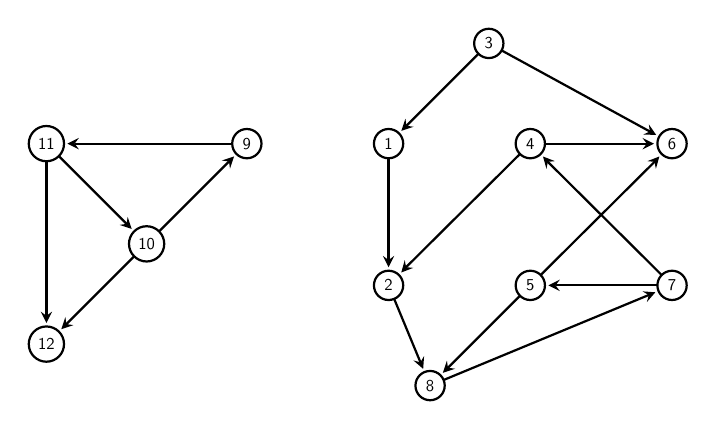
\begin{tikzpicture}[->,>=stealth,shorten >=1pt,auto,node distance=3cm,thick,main node/.style={scale=0.6,circle,draw,font=\sffamily\normalsize}]
                        \node[main node] (1) {1};
                        \node[main node] (2) [below of=1]{2};
                        \node[main node] (3) [above right of=1]{3};
                        \node[main node] (4) [right of=1]{4};
                        \node[main node] (5) [below of=4]{5};
                        \node[main node] (6) [right of=4]{6};
                        \node[main node] (7) [right of=5]{7};
                        \node[main node] (8) [below left of=5]{8};
                        \node[main node] (9) [left of=1]{9};
                        \node[main node] (10) [below left of=9]{10};
                        \node[main node] (11) [above left of=10]{11};
                        \node[main node] (12) [below left of=10]{12};
        
                        \path[every node/.style={font=\sffamily\small}]
                            (1) edge (2)
                            (3) edge (1)
                            (2) edge (8)
                            (8) edge (7)
                            (5) edge (8)
                            (4) edge (2)
                            (7) edge (4)
                            (3) edge (6)
                            (5) edge (6)
                            (4) edge (6)
                            (7) edge (5)
        
                            (11) edge (10)
                            (11) edge (12)
                            (10) edge (9)
                            (10) edge (12)
                            (9) edge (11)
                        ;
        
                    \end{tikzpicture}
                \end{tabular}

                &\qquad&

                \begin{tabular}{c|c}
                    \textbf{Vertice} & \textbf{\ttt{Comp}}\\
                    \hline
                    1 & 0\\
                    2 & 0\\
                    3 & 0\\
                    4 & 0\\
                    5 & 0\\
                    6 & 0\\
                    7 & 0\\
                    8 & 0\\
                    9 & 0\\
                    10 & 0\\
                    11 & 0\\
                    12 & 0\\
                \end{tabular}
            \end{tabular}
        \end{center}

        \newpage

        \item Eseguiamo la prima DFS dell'algoritmo, partendo dal vertice $3$
        \begin{center}
            \begin{tabular}{ccc}
                \begin{tabular}{c}
                    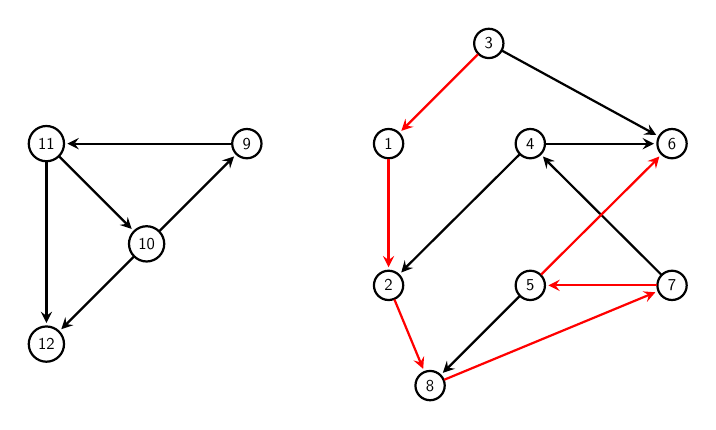
\begin{tikzpicture}[->,>=stealth,shorten >=1pt,auto,node distance=3cm,thick,main node/.style={scale=0.6,circle,draw,font=\sffamily\normalsize}]
                        \node[main node] (1) {1};
                        \node[main node] (2) [below of=1]{2};
                        \node[main node] (3) [above right of=1]{3};
                        \node[main node] (4) [right of=1]{4};
                        \node[main node] (5) [below of=4]{5};
                        \node[main node] (6) [right of=4]{6};
                        \node[main node] (7) [right of=5]{7};
                        \node[main node] (8) [below left of=5]{8};
                        \node[main node] (9) [left of=1]{9};
                        \node[main node] (10) [below left of=9]{10};
                        \node[main node] (11) [above left of=10]{11};
                        \node[main node] (12) [below left of=10]{12};

                        \path[every node/.style={font=\sffamily\small}]
                            (5) edge (8)
                            (4) edge (2)
                            (7) edge (4)
                            (3) edge (6)
                            (4) edge (6)

                            (11) edge (10)
                            (11) edge (12)
                            (10) edge (9)
                            (10) edge (12)
                            (9) edge (11)
                        ;

                        \path[every node/.style={font=\sffamily\small}]
                            [color=red]
                            (3) edge (1)
                            (1) edge (2)
                            (2) edge (8)
                            (8) edge (7)
                            (7) edge (5)
                            (5) edge (6)
                        ;

                    \end{tikzpicture}
                \end{tabular}

                &\qquad&

                \begin{tabular}{c|c}
                    \textbf{Vertice} & \textbf{\ttt{Comp}}\\
                    \hline
                    1 & -2\\
                    2 & -3\\
                    3 & 1\\
                    4 & 0\\
                    5 & -6\\
                    6 & -7\\
                    7 & -5\\
                    8 & -4\\
                    9 & 0\\
                    10 & 0\\
                    11 & 0\\
                    12 & 0\\
                \end{tabular}
            \end{tabular}
        \end{center}

        (ricordiamo che \texttt{Comp[$x$] < 0} $\implies$ \texttt{Comp[$x$] = $-t(x)$})

        \item Poiché il vertice $6$ non ha archi uscenti, ne segue che \texttt{back}$_6 = t(6) = 7$, implicando quindi che \texttt{back}$_6 = -$\texttt{Comp[$6$]} e dunque che $6$ sia c-radice di $comp(6)$.
        
        Di conseguenza, tutti i vertici aggiunti allo stack dopo $6$ (ossia nessun altro vertice) appartiene a $comp(6)$, venendo rimossi dallo stack e marchiati con valore attuale del contatore $cc$, ossia $1$

        \begin{center}
            \begin{tabular}{ccc}
                \begin{tabular}{c}
                    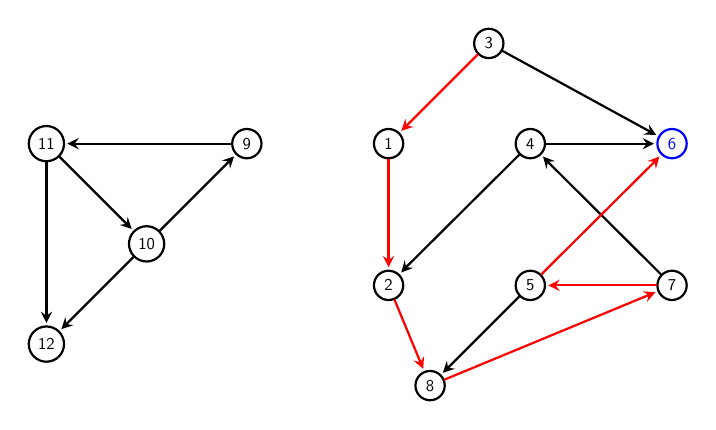
\begin{tikzpicture}[->,>=stealth,shorten >=1pt,auto,node distance=3cm,thick,main node/.style={scale=0.6,circle,draw,font=\sffamily\normalsize}]
                        \node[main node] (1) {1};
                        \node[main node] (2) [below of=1]{2};
                        \node[main node] (3) [above right of=1]{3};
                        \node[main node] (4) [right of=1]{4};
                        \node[main node] (5) [below of=4]{5};
                        \node[main node] (6) [color=blue, right of=4]{6};
                        \node[main node] (7) [right of=5]{7};
                        \node[main node] (8) [below left of=5]{8};
                        \node[main node] (9) [left of=1]{9};
                        \node[main node] (10) [below left of=9]{10};
                        \node[main node] (11) [above left of=10]{11};
                        \node[main node] (12) [below left of=10]{12};

                        \path[every node/.style={font=\sffamily\small}]
                            (5) edge (8)
                            (4) edge (2)
                            (7) edge (4)
                            (3) edge (6)
                            (4) edge (6)

                            (11) edge (10)
                            (11) edge (12)
                            (10) edge (9)
                            (10) edge (12)
                            (9) edge (11)
                        ;

                        \path[every node/.style={font=\sffamily\small}]
                            [color=red]
                            (3) edge (1)
                            (1) edge (2)
                            (2) edge (8)
                            (8) edge (7)
                            (7) edge (5)
                            (5) edge (6)
                        ;

                    \end{tikzpicture}
                \end{tabular}

                &\qquad&

                \begin{tabular}{c|c}
                    \textbf{Vertice} & \textbf{\ttt{Comp}}\\
                    \hline
                    1 & -2\\
                    2 & -3\\
                    3 & -1\\
                    4 & 0\\
                    5 & -6\\
                    6 & 1\\
                    7 & -5\\
                    8 & -4\\
                    9 & 0\\
                    10 & 0\\
                    11 & 0\\
                    12 & 0\\
                \end{tabular}
            \end{tabular}
        \end{center}

        \item Proseguiamo quindi la DFS ricorsiva avente $3$ come radice, tornando al vertice $5$. Poiché $(5,8) \in E(G)$ e $8$ è già stato visitato ma non chiuso, ne segue che \texttt{back}$_5 = t(8) = 4$, ritornando tale valore alla chiamata precedente, ossia la visita del vertice $7$. Inoltre, poiché \texttt{back}$_5 = t(8) = 4 <$ \texttt{back}$_7 =t(7) = 5$, viene sovrascritto \texttt{back}$_7 = t(8)$.
        
        \item Successivamente, la DFS procederà verso il vertice $4$, ponendo \ttt{Comp[$4$] = $-8$}. Poiché $(4,2) \in E(G)$ e $2$ è stato già visitato ma non ancora chiuso, si ha che \texttt{back}$_4 = t(2) = 3$, ritornando tale valore al vertice $7$ e sovrascrivendo \texttt{back}$_7 = t(2)$ poiché \texttt{back}$_4 = t(2) = 3 <$ \texttt{back}$_7 =t(8) = 4$.

        \item Poiché $7$ non ha altri vertici adiacenti, il valore \texttt{back}$_7 = t(2)$ viene ritornato alla visita del vertice $8$. Poiché \texttt{back}$_7 = t(2) = 3 <$ \texttt{back}$_8 =t(8) = 4$, viene sovrascritto \texttt{back}$_8 = t(2)$. Analogamente, poiché $8$ non ha altri vertici adiacenti, il valore \texttt{back}$_8 = t(2)$ viene ritornato alla visita del vertice $2$. Poiché \texttt{back}$_8 = t(2) =$ \texttt{back}$_2 =-$ \texttt{Comp[$2$]}, l'algoritmo determina che $2$ sia la c-radice di $comp(2)$.

        Di conseguenza, tutti i vertici aggiunti allo stack dopo $2$, ossia $8,7,5$ vengono rimossi dallo stack e marchiati con valore attuale del contatore $cc$, ossia $2$

        \begin{center}
            \begin{tabular}{ccc}
                \begin{tabular}{c}
                    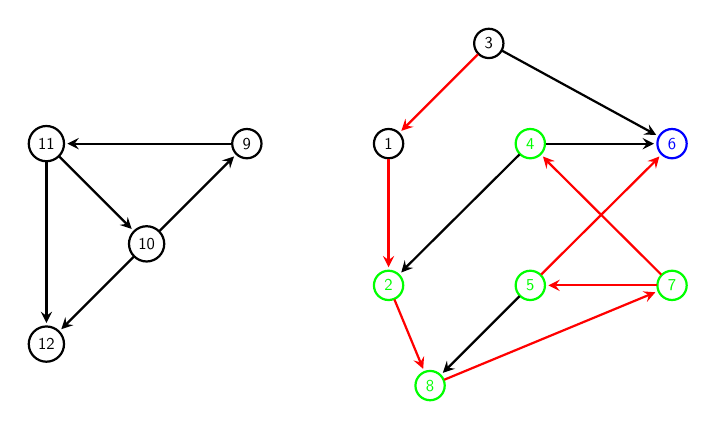
\begin{tikzpicture}[->,>=stealth,shorten >=1pt,auto,node distance=3cm,thick,main node/.style={scale=0.6,circle,draw,font=\sffamily\normalsize}]
                        \node[main node] (1) {1};
                        \node[main node] (2) [color=green,below of=1]{2};
                        \node[main node] (3) [above right of=1]{3};
                        \node[main node] (4) [color=green,right of=1]{4};
                        \node[main node] (5) [color=green, below of=4]{5};
                        \node[main node] (6) [color=blue, right of=4]{6};
                        \node[main node] (7) [color=green,right of=5]{7};
                        \node[main node] (8) [color=green,below left of=5]{8};
                        \node[main node] (9) [left of=1]{9};
                        \node[main node] (10) [below left of=9]{10};
                        \node[main node] (11) [above left of=10]{11};
                        \node[main node] (12) [below left of=10]{12};

                        \path[every node/.style={font=\sffamily\small}]
                            (5) edge (8)
                            (4) edge (2)
                            (3) edge (6)
                            (4) edge (6)

                            (11) edge (10)
                            (11) edge (12)
                            (10) edge (9)
                            (10) edge (12)
                            (9) edge (11)
                        ;

                        \path[every node/.style={font=\sffamily\small}]
                            [color=red]
                            (3) edge (1)
                            (1) edge (2)
                            (2) edge (8)
                            (8) edge (7)
                            (7) edge (5)
                            (5) edge (6)
                            (7) edge (4)
                        ;

                    \end{tikzpicture}
                \end{tabular}

                &\qquad&

                \begin{tabular}{c|c}
                    \textbf{Vertice} & \textbf{\ttt{Comp}}\\
                    \hline
                    1 & -2\\
                    2 & 2\\
                    3 & -1\\
                    4 & 2\\
                    5 & 2\\
                    6 & 1\\
                    7 & 2\\
                    8 & 2\\
                    9 & 0\\
                    10 & 0\\
                    11 & 0\\
                    12 & 0\\
                \end{tabular}
            \end{tabular}
        \end{center}

        \item Una volta tornati alla visita di $1$, poiché esso non ha altri vertici adiacenti ne segue che \texttt{back}$_1 = -$\texttt{Comp[$1$]}, dunque $1$ è la c-radice di $comp(1)$, rimuovendo dallo stack e marchiando con $cc=3$ gli elementi inseriti dopo di esso nello stack (nessuno).
        
        Analogamente, $3$ risulta essere la c-radice di $3$, dunque si ha che.

        \begin{center}
            \begin{tabular}{ccc}
                \begin{tabular}{c}
                    \begin{tikzpicture}[->,>=stealth,shorten >=1pt,auto,node distance=3cm,thick,main node/.style={scale=0.6,circle,draw,font=\sffamily\normalsize}]
                        \node[main node] (1) [color=purple]{1};
                        \node[main node] (2) [color=green,below of=1]{2};
                        \node[main node] (3) [color=orange, above right of=1]{3};
                        \node[main node] (4) [color=green,right of=1]{4};
                        \node[main node] (5) [color=green, below of=4]{5};
                        \node[main node] (6) [color=blue, right of=4]{6};
                        \node[main node] (7) [color=green,right of=5]{7};
                        \node[main node] (8) [color=green,below left of=5]{8};
                        \node[main node] (9) [left of=1]{9};
                        \node[main node] (10) [below left of=9]{10};
                        \node[main node] (11) [above left of=10]{11};
                        \node[main node] (12) [below left of=10]{12};

                        \path[every node/.style={font=\sffamily\small}]
                            (5) edge (8)
                            (4) edge (2)
                            (3) edge (6)
                            (4) edge (6)

                            (11) edge (10)
                            (11) edge (12)
                            (10) edge (9)
                            (10) edge (12)
                            (9) edge (11)
                        ;

                        \path[every node/.style={font=\sffamily\small}]
                            [color=red]
                            (3) edge (1)
                            (1) edge (2)
                            (2) edge (8)
                            (8) edge (7)
                            (7) edge (5)
                            (5) edge (6)
                            (7) edge (4)
                        ;

                    \end{tikzpicture}
                \end{tabular}

                &\qquad&

                \begin{tabular}{c|c}
                    \textbf{Vertice} & \textbf{\ttt{Comp}}\\
                    \hline
                    1 & 3\\
                    2 & 2\\
                    3 & 4\\
                    4 & 2\\
                    5 & 2\\
                    6 & 1\\
                    7 & 2\\
                    8 & 2\\
                    9 & 0\\
                    10 & 0\\
                    11 & 0\\
                    12 & 0\\
                \end{tabular}
            \end{tabular}
        \end{center}

        \item A questo punto, la DFS avente $3$ come radice termina. Di conseguenza, viene effettuata una nuova DFS su uno dei vertici non ancora esplorati (sceglieremo il vertice $10$).

        \begin{center}
            \begin{tabular}{ccc}
                \begin{tabular}{c}
                    \begin{tikzpicture}[->,>=stealth,shorten >=1pt,auto,node distance=3cm,thick,main node/.style={scale=0.6,circle,draw,font=\sffamily\normalsize}]
                        \node[main node] (1) [color=purple]{1};
                        \node[main node] (2) [color=green,below of=1]{2};
                        \node[main node] (3) [color=orange, above right of=1]{3};
                        \node[main node] (4) [color=green,right of=1]{4};
                        \node[main node] (5) [color=green, below of=4]{5};
                        \node[main node] (6) [color=blue, right of=4]{6};
                        \node[main node] (7) [color=green,right of=5]{7};
                        \node[main node] (8) [color=green,below left of=5]{8};
                        \node[main node] (9) [left of=1]{9};
                        \node[main node] (10) [below left of=9]{10};
                        \node[main node] (11) [above left of=10]{11};
                        \node[main node] (12) [below left of=10]{12};

                        \path[every node/.style={font=\sffamily\small}]
                            (5) edge (8)
                            (4) edge (2)
                            (3) edge (6)
                            (4) edge (6)
                            (3) edge (1)
                            (1) edge (2)
                            (2) edge (8)
                            (8) edge (7)
                            (7) edge (5)
                            (5) edge (6)
                            (7) edge (4)

                            (11) edge (10)
                            (10) edge (12)
                        ;

                        \path[every node/.style={font=\sffamily\small}]
                            [color=red]
                            (10) edge (9)
                            (9) edge (11)
                            (11) edge (12)
                        ;

                    \end{tikzpicture}
                \end{tabular}

                &\qquad&

                \begin{tabular}{c|c}
                    \textbf{Vertice} & \textbf{\ttt{Comp}}\\
                    \hline
                    1 & 3\\
                    2 & 2\\
                    3 & 4\\
                    4 & 2\\
                    5 & 2\\
                    6 & 1\\
                    7 & 2\\
                    8 & 2\\
                    9 & -10\\
                    10 & -9\\
                    11 & -11\\
                    12 & -12\\
                \end{tabular}
            \end{tabular}
        \end{center}

        \item Analogamente a $1,3$ e $6$, il vertice $12$ risulta essere la c-radice di $comp(12)$, marchiando i suoi elementi con $cc=5$. Infine, analogamente al vertice $2$, il vertice $10$ viene decretato c-radice di $comp(10)$, marchiando i suoi elementi con $cc=6$

        \begin{center}
            \begin{tabular}{ccc}
                \begin{tabular}{c}
                    \begin{tikzpicture}[->,>=stealth,shorten >=1pt,auto,node distance=3cm,thick,main node/.style={scale=0.6,circle,draw,font=\sffamily\normalsize}]
                        \node[main node] (1) [color=purple]{1};
                        \node[main node] (2) [color=green,below of=1]{2};
                        \node[main node] (3) [color=orange, above right of=1]{3};
                        \node[main node] (4) [color=green,right of=1]{4};
                        \node[main node] (5) [color=green, below of=4]{5};
                        \node[main node] (6) [color=blue, right of=4]{6};
                        \node[main node] (7) [color=green,right of=5]{7};
                        \node[main node] (8) [color=green,below left of=5]{8};
                        \node[main node] (9) [color=cyan, left of=1]{9};
                        \node[main node] (10) [color=cyan, below left of=9]{10};
                        \node[main node] (11) [color=cyan, above left of=10]{11};
                        \node[main node] (12) [color=gray, below left of=10]{12};

                        \path[every node/.style={font=\sffamily\small}]
                            (5) edge (8)
                            (4) edge (2)
                            (3) edge (6)
                            (4) edge (6)
                            (3) edge (1)
                            (1) edge (2)
                            (2) edge (8)
                            (8) edge (7)
                            (7) edge (5)
                            (5) edge (6)
                            (7) edge (4)

                            (11) edge (10)
                            (10) edge (12)
                        ;

                        \path[every node/.style={font=\sffamily\small}]
                            [color=red]
                            (10) edge (9)
                            (9) edge (11)
                            (11) edge (12)
                        ;

                    \end{tikzpicture}
                \end{tabular}

                &\qquad&

                \begin{tabular}{c|c}
                    \textbf{Vertice} & \textbf{\ttt{Comp}}\\
                    \hline
                    1 & 3\\
                    2 & 2\\
                    3 & 4\\
                    4 & 2\\
                    5 & 2\\
                    6 & 1\\
                    7 & 2\\
                    8 & 2\\
                    9 & 6\\
                    10 & 6\\
                    11 & 6\\
                    12 & 5\\
                \end{tabular}
            \end{tabular}
        \end{center}

        \item Poiché non vi sono altri vertici visitabili, tramite l'array \texttt{Comp} concludiamo che
        \begin{itemize}
            \item $comp(1) = \{1\}$
            \item $comp(2) = \{2,4,5,7,8\}$
            \item $comp(3) = \{3\}$
            \item $comp(10) = \{9,10,11\}$
            \item $comp(12) = \{12\}$
        \end{itemize}
    \end{itemize}

    \section{Breadth-first Search (BFS)}

    \quad

    \begin{frameddefn}{Breadth-first Search (BFS)}
        Sia $G $ un grafo. Dato un vertice iniziale $x \in V(G)$ definiamo come \textbf{breadth-first search (BFS)} un \textbf{criterio di visita} su $G$ basato sul procedere \textbf{in ampiezza}, ossia dando precedenza ai vertici più vicini dal vertice iniziale, raggiungendo ogni vertice \textbf{una ed una sola volta}, procedendo con il vertice successivo \underline{se e solo se} non è più possibile procedere in ampiezza tramite il vertice attuale, ossia quando tutti i vertici adiacenti sono già stati visitati
    \end{frameddefn}

    \textbf{Esempio:}

    \begin{itemize}
        \item Dato il seguente grafico, eseguendo una DFS sul vertice $6$ otterremmo la seguente arborescenza con il seguente ordine di visita $[6,5,2,3,4,1]$ 
        
        \begin{center}
            \begin{tikzpicture}[-,>=stealth,shorten >=1pt,auto,node distance=3cm,thick,main node/.style={scale=0.6,circle,draw,font=\sffamily\normalsize}]
                \node[main node] (1) {1};
                \node[main node] (2) [above of=1] {2};
                \node[main node] (3) [right of=2] {3};
                \node[main node] (4) [left of=1] {4};
                \node[main node] (5) [right of=1] {5};
                \node[main node] (6) [below of=1] {6};

                \path[every node/.style={font=\sffamily\small}]
                    (3) edge (5)
                    (6) edge (4)
                    (6) edge (1)
                    (1) edge (5)
                    ;
                \path[every node/.style={font=\sffamily\small}]
                    [color=red]
                    (6) edge (5)
                    (5) edge (2)
                    (2) edge (3)
                    (3) edge (4)
                    (1) edge (2)
                    ;
            \end{tikzpicture}
        \end{center}

        \item Eseguiamo invece una BFS su $6$, dando quindi precedenza a tutti i suoi archi uscenti, ossia $(6,5), (6,1), (6,4)$
        
        \begin{center}
            \begin{tikzpicture}[-,>=stealth,shorten >=1pt,auto,node distance=3cm,thick,main node/.style={scale=0.6,circle,draw,font=\sffamily\normalsize}]
                \node[main node] (1) {1};
                \node[main node] (2) [above of=1] {2};
                \node[main node] (3) [right of=2] {3};
                \node[main node] (4) [left of=1] {4};
                \node[main node] (5) [right of=1] {5};
                \node[main node] (6) [below of=1] {6};

                \path[every node/.style={font=\sffamily\small}]
                    
                    (2) edge (3)
                    (3) edge (4)
                    (1) edge (2)
                    (5) edge (2)
                    (3) edge (5)
                    (1) edge (5)
                    ;
                \path[every node/.style={font=\sffamily\small}]
                    [color=green]
                    (6) edge (5)
                    (6) edge (1)
                    (6) edge (4)
                    ;
            \end{tikzpicture}
        \end{center}

        \item A questo punto, procediamo con il prossimo vertice, ossia $5$, dando quindi precedenza agli archi $(5,2), (5,3)$. A questo punto, poiché non vi sono altri vertici visitabili, la BFS termina con il seguente ordine di visita $[6,5,1,4,2,3]$ 
        
        \begin{center}
            
        \end{center}
    \end{itemize}

    \begin{frameddefn}{Distanza tra vertici}
        Sia $G$ un grafo. Dati due vertici $x,y \in V(G)$, definiamo come \textbf{distanza tra $x$ e $y$}, indicata come $dist(x,y)$, il numero minimo di archi appartenenti ad un cammino tale che $x \to y$

        Se non esiste un cammino tale che $x \to y$, diciamo che $dist(x,y) = +\infty$
    \end{frameddefn}

    \begin{framedprop}{}
        Sia $G$ un grafo. Dato un vertice $x \in V(G)$, si ha che:
        \[\forall y \neq x \in V(G), \exists z \in V(G) \mid (z,y) \in E(G), dist(x,y)=dist(x,z)+1\]

    \end{framedprop}

    \textit{Dimostrazione:}

    \begin{itemize}
        \item Sia $dist(x,y)= L$, implicando che esista un cammino $x e_1 v_1 e_2 \ldots e_{L-1} v_{L-1} e_{L} y$ di lunghezza minima tale che $x \to y$.
        \item Posti $z := v_{L-1}$ e $k := dist(x,z)$, se per assurdo $x e_1 v_1 e_2 \ldots e_{L-1} z$ non fosse un cammino di lunghezza minima tale che $x \to z$, esisterebbe un cammino di lunghezza minima $x h_1 u_1 e_2 \ldots e_{k} z$ tale che $x \to z$ dove $k < L-1$, implicando che $x h_1 u_1 h_2 \ldots h_{k} z e_L y$ sia un cammino di lunghezza $k+1 < L$ tale che $x \to y$, contraddicendo l'ipotesi per cui $dist(x,y)=L$
        \item Di conseguenza, l'unica possibilità è che
        \[dist(x,z) = L-1 = dist(x,y) -1 \implies dist(x,y) = dist(x,z)+1\]
        $\hfill\qed$
    \end{itemize}

    \begin{frameddefn}{Livello di un vertice}
        Sia $T$ un albero radicato o un'arborescenza radicata, dove $u \in V(G)$ è la radice. Dato un vertice $v \in V(G)$, definiamo $L := dist(u,v)$ come \textbf{livello di $v$} 
    \end{frameddefn}

    \begin{framedalgo}{Breadth-first Search}
        Sia $G$ un grafo rappresentato tramite liste di adiacenza. Dato un vertice $x \in V(G)$, il seguente algoritmo restituisce la distanza $dist(x,y)$ per ogni vertice $y \in V(G)$ raggiunto da una BFS su $x$ e il vettore dei padri rappresentante l'albero/arborescenza di visita generato
        
        Il \textbf{costo} risulta essere $O(n+m)$, dove $\abs{V(G)}=n$ e $\abs{E(G)}=m$
    \end{framedalgo}

    \begin{algorithm}[H]
        \caption{Breadth-first Search}\label{bfs}
        \KwIn{\\
        G: grafo a liste di adiacenza,\\
        u: $u \in V(G)$,\\
        }
        \KwOut{\\
        Distanze dalla radice dei vertici visitati e
        albero/arborescenza di visita tramite vettore dei padri}
        
        \Fn{\texttt{\upshape BFS(G, $u$):}}{
            \texttt{Padri = [-1, ..., -1]}\;
            \texttt{Dist = [-1, ..., -1]}\;
            \texttt{\textbf{Queue} Q = $\varnothing$}\;
            \texttt{Q.enqueue($u$)}\;
            \texttt{Padri[$u$] = $u$}\;
            \texttt{Dist[$u$] = 0}\;
            \While{\texttt{Q $\neq \varnothing$}}{
                \texttt{$v$ = Q.dequeue()}\;
                \For{\texttt{$x\in v$.uscenti}}{
                    \If{\texttt{Dist[$x$] = $-1$}}{
                        \texttt{Padri[$x$] = $v$}\;
                        \texttt{Dist[$x$] = Dist[$v$] + $1$}\;
                        \texttt{Q.enqueue($x$)}\;
                    }
                }
            }
            \texttt{return Dist, Padri}\;
        }
    \end{algorithm}

    \textit{Dimostrazione correttezza e costo algoritmo:}
    \begin{itemize}
        \item Posto \texttt{Dist[$u$] = 0}, la radice $u$ è il primo vertice inserito e rimosso dalla queue. 
        \item Siano quindi $x_1, \ldots, x_k \in V(G)$ i vertici adiacenti alla radice tali che $(u, x_i) \in E(G), \forall i \in [1,k]$, implicando che $dist(u,x_i) = 1, \forall i \in [1,k]$. Poiché \texttt{Dist[$u$] = 0}, ne segue che \texttt{Dist[$x_i$] = Dist[$u$] + 1 = 1}, $\forall i \in [1,k]$
        \item Assumiamo quindi per ipotesi induttiva che \texttt{Dist[$v$] = $dist(u, v)$} per ogni vertice $v \in V(G)$ rimosso dalla queue.
        \item Dato il vertice $z \in V(G)$ tale che $dist(u,z) = k+1$, per la proposizione precedente $\exists y \in V(G) \mid (y,z) \in E(G), dist(u,z) = dist(u,y) +1$, implicando che $z$ verrà visitato dalla BFS nel momento in cui $y$ verrà rimosso dalla queue.
        
        \item Per ipotesi induttiva, dunque, ne segue che \texttt{Dist[$y$] = $dist(u,y)$ = $dist(u,z) -1 = k$}, implicando quindi che \texttt{Dist[$z$] = Dist[$y$] + 1 = k+1 = $dist(u,z)$}
        
        \item Il calcolo del costo computazionale di una BFS risulta analogo al calcolo per una DFS. Di conseguenza, il costo dell'algoritmo è $O(n+m)$
        
        $\hfill\qed$
    \end{itemize}

    \newpage

    \section{Esercizi svolti}

    \begin{framedprob}{Trovare numero di cammini minimi dalla radice}
        Dato un grafo $G$ e un vertice $x \in V(G)$, per ogni vertice $y \in V(G)$ vogliamo trovare il numero di camini di lunghezza minima tale che $x \to y$
    \end{framedprob}

    \begin{algorithm}[H]
        \KwIn{\\
        G: grafo a liste di adiacenza, u: $u \in V(G)$\\
        }
        \KwOut{\\
        Numero di cammini minimi dalla radice di ogni vertice visitabile}
        
        \Fn{\texttt{\upshape countMinPaths(G, $u$):}}{
            \texttt{Dist = [-1, ..., -1]}\;
            \texttt{Count = [0, ..., 0]}\;
            \texttt{\textbf{Queue} Q = $\varnothing$}\;
            \texttt{Q.enqueue($u$)}\;
            \texttt{Dist[$u$] = 0}\;
            \texttt{Count[$u$] = 1}\;
            \While{\texttt{Q $\neq \varnothing$}}{
                \texttt{$v$ = Q.dequeue()}\;
                \For{\texttt{$x\in v$.uscenti}}{
                    \uIf{\texttt{Dist[$x$] = $-1$}}{
                        \texttt{Dist[$x$] = Dist[$v$] + $1$}\;
                        \texttt{Count[$x$] = Count[$v$]}\;
                        \texttt{Q.enqueue($x$)}\;
                    }
                    \uElseIf{\texttt{Dist[$v$] = Dist[$x$] - 1}}{
                        \texttt{Count[$x$] += Count[$v$]}\;
                    }
                }
            }
            \texttt{return Count}\;
        }
    \end{algorithm}
    
    \label{process}

    \begin{framedprob}{Programmazione di un processo di produzione}
        Una fabbrica ha diviso un processo di produzione in $n$ fasi. Tra alcune coppie di fasi vi è una dipendenza, ossia una di esse deve essere completata prima dell'altra. Vogliamo trovare una possibile programmazione (se esistente) del processo di produzione rispettante tutte le dipendenze.
    \end{framedprob}

    \textit{Soluzione:}

    \begin{itemize}
        \item Siano $V(G) := x_1, \ldots, x_n$ le fasi del processo di produzione. Modelliamo le dipendenze tra ogni fase come degli archi diretti, dove $\exists (x_i,x_j) \in E(G) \iff x_j \text{ dipende da } x_i$
        
        Possiamo quindi tradurre la richiesta nel trovare un ordine topologico di $G$.
        
        \item Per dimostrazione precedente, sappiamo che ha che $\exists \text{ ordine topologico in }G \iff \nexists \text{ ciclo in }G$
        dunque, abbiamo che:
        \begin{itemize}
            \item Se l'algoritmo \ref{findCycle_2} \texttt{findCycle} trova un ciclo, allora non esiste una soluzione
            \item Se l'algoritmo \ref{findCycle_2} \texttt{findCycle} non trova un ciclo, allora $G$ è un DAG, implicando che la soluzione sia data dall'algoritmo \ref{ord_top_2} \texttt{findTopologicalSorting}
        \end{itemize}
        
        \item Il grafo è modellabile in tempo $O(n+m)$, ossia lo stesso costo di entrambi gli algoritmi, rendendo il problema è risolvibile in $O(n+m$)
    \end{itemize}

    \begin{framedprob}{Distanza tra sotto-insiemi di vertici}
        Dato un grafo $G$ e due sotto-insiemi $X, Y \subseteq V(G)$, definiamo:
        \[dist(X, Y) = \min_{x \in X, y \in Y} dist(x,y)\]
        
        Progettare un algoritmo che in $O(n+m)$ trovi la distanza tra $X$ e $Y$, restituendo $dist(X,Y) = +\infty$ se non esiste un cammino da $x \in X$ a $y \in Y$
    \end{framedprob}

    \begin{algorithm}[H]
        \KwIn{\\
        G: grafo a liste di adiacenza, X: $X \subseteq V(G)$, Y: $Y \subseteq V(G)$\\
        }
        \KwOut{\\
        Distanza tra X e Y}
        
        \Fn{\texttt{\upshape distBetweenSubsets(G, X, Y):}}{
            \texttt{Dist = [-1, ..., -1]}\;
            \texttt{\textbf{Queue} Q = $\varnothing$}\;
            \For{$x \in X$}{
                \texttt{Q.enqueue($x$)}\;
                \texttt{Dist[$x$] = 0}\;
            }
            \While{\texttt{Q $\neq \varnothing$}}{
                \texttt{$u$ = Q.dequeue()}\;
                \For{\texttt{$v\in u$.uscenti}}{
                    \uIf{\texttt{Dist[$v$] = $-1$}}{
                        \texttt{Dist[$v$] = Dist[$u$] + $1$}\;
                        \texttt{Q.enqueue($x$)}\;
                    }
                }
            }
            \texttt{minDist = $+\infty$}\;
            \For{$y \in Y$}{
                \uIf{\texttt{Dist[$y$] < minDist}}{
                    \texttt{minDist = Dist[$y$]}\;
                }
            }
            \texttt{return minDist}\;
        }
    \end{algorithm}

    \newpage

    \begin{framedprob}{Minimo Antenato Comune}
        Dato in input un albero $T$ rappresentato tramite vettore dei padri $P[\,]$ e tre vertici $x,y,z \in V(T)$, progettare un algoritmo che in $O(n)$ restituisca il minimo antenato comune (Lowest Common Ancestor - LCA) dei vertici $x,y$ e $z$.

        \textit{\textbf{Nota:}} con $LCA(x,y,z)$ si intende l'antenato in comune tra i tre vertici più distante dalla radice
    \end{framedprob}

    \begin{algorithm}[H]
        \KwIn{\\
        P: vettore dei padri di un albero $T$,\\
        x, y, z: vertici di $V(T)$\\
        }
        \KwOut{\\
        Minimo antenato comune di $x$, $y$ e $z$}
        \Fn{\texttt{\upshape distFromRadix(P, v):}}{
            \texttt{$d$ = 0}\;
            \While{\texttt{v $\neq$ P[v]}}{
                \texttt{$d++$}\;
                \texttt{$v = P[v]$}\;
            }
            \texttt{return $d$}\;
        }
        \Fn{\texttt{\upshape LCA(P, x, y, z):}}{
            \texttt{$d_x$ = distFromRadix(P, $x$)}\;
            \texttt{$d_y$ = distFromRadix(P, $y$)}\;
            \texttt{$d_z$ = distFromRadix(P, $z$)}\;
            \While{\texttt{\textbf{not} ($d_x$ == $d_y$ == $d_z$)}}{
                \texttt{maxDist = max($d_x$, $d_y$, $d_z$)}\;
                \uIf{\texttt{maxDist == $d_x$}}{
                    \texttt{$x$ = P[$x$]}\;
                    \texttt{$d_x--$}\;
                }
                \uElseIf{\texttt{maxDist == $d_y$}}{
                    \texttt{$y$ = P[$y$]}\;
                    \texttt{$d_y--$}\;
                }
                \uElse{
                    \texttt{$z$ = P[$z$]}\;
                    \texttt{$d_z--$}\;
                }
            }
            \While{\texttt{\textbf{not} ($x$ == $y$ == $z$)}}{
                \texttt{$x$ = P[$x$]}\;
                \texttt{$y$ = P[$y$]}\;
                \texttt{$z$ = P[$z$]}\;
            }
            \texttt{return $x$}\;
        }
    \end{algorithm}


    \begin{framedprob}{Distanza tra due vertici in un albero}
        Dato in input un albero $T$ rappresentato tramite vettore dei padri $P[\,]$ e due vertici $x,y \in V(T)$, progettare un algoritmo che in $O(n)$ restituisca $dist(x,y)$
    \end{framedprob}

    \begin{algorithm}[H]
        \KwIn{\\
        P: vettore dei padri di un albero $T$,\\
        x, y: vertici di $V(T)$\\
        }
        \KwOut{\\
        Distanza tra $x$ e $y$}
        
        \Fn{\texttt{\upshape distFromRadix(P, v):}}{
            \texttt{$d$ = 0}\;
            \While{\texttt{v $\neq$ P[v]}}{
                \texttt{$d++$}\;
                \texttt{$v = P[v]$}\;
            }
            \texttt{return $d$}\;
        }
        \Fn{\texttt{\upshape vertexDistance(P, x, y):}}{
            \texttt{$d_x$ = distFromRadix(P, $x$)}\;
            \texttt{$d_y$ = distFromRadix(P, $y$)}\;
            \texttt{$t_x$ = $d_x$}\;
            \texttt{$t_y$ = $d_y$}\;
            \While{\texttt{$t_x \neq t_y$}}{
                \eIf{\texttt{$d_x$ > $d_y$}}{
                    \texttt{$x$ = P[$x$]}\;
                    \texttt{$t_x--$}\;
                }
                {
                    \texttt{$y$ = P[$y$]}\;
                    \texttt{$t_y--$}\;
                }
            }
            \While{\texttt{$x \neq y$}}{
                \texttt{$x$ = P[$x$]}\;
                \texttt{$y$ = P[$y$]}\;
                \texttt{$t_x--$}\;
            }
            \texttt{return $d_x + d_y - 2 \cdot t_x$}\qquad //$t_x$ è attualmente la distanza di LCA(x,y)\;
        }
    \end{algorithm}

    \chapter{Algoritmi Greedy}

    \quad

    \section{Definizione e scheletro di dimostrazione}

    \quad

    \begin{frameddefn}{Algoritmo Greedy}
        Un algoritmo viene detto \textbf{greedy} se cerca una soluzione ammissibile da un punto di vista globale attraverso la scelta della soluzione più conveniente ad ogni passo locale
    \end{frameddefn}

    \begin{framedobs}{}
        Sebbene spesso gli algoritmi greedy risultino essere molto brevi e coincisi, è sempre necessario dimostrare che l'output generato sia una \textbf{soluzione ottimale}, ossia una soluzione rispettante la richiesta dell'algoritmo
    \end{framedobs}

    Il seguente \textbf{scheletro di dimostrazione} fornisce una base per dimostrare la correttezza di un algoritmo greedy:
    \begin{enumerate}
        \item Dimostrare che l'output rispetti le \textbf{caratteristiche previste}
        \item Dimostrare per induzione che ogni istanza dell'output (ossia il suo contenuto a seguito di ogni iterazione) sia \textbf{contenuto all'interno di una qualsiasi soluzione ottimale}:
        \begin{itemize}
            \item Supponendo che l'istanza \texttt{Sol}$_k$ sia contenuta in una soluzione ottimale \texttt{Sol}$^*$, dimostrare che anche \texttt{Sol}$_{k+1}$ sia contenuto in una soluzione ottimale, la quale solitamente coincide con $(\texttt{Sol}^*-x) \cup y$, dove $x \in \texttt{Sol}^*$ e $y \notin \texttt{Sol}^*$
        \end{itemize}
        \item Dimostrare che l'output finale generato \textbf{coincida esattamente con la soluzione ottimale} all'interno di cui è contenuto
    \end{enumerate}

    \subsection{Esempi di dimostrazione di algoritmi greedy}

    \quad

    \begin{framedprob}{Massimi intervalli disgiunti}
        Dato un insieme di $n$ intervalli nella forma $[a_i, b_i]$, dare un algoritmo che trovi un sotto-insieme di cardinalità massima di intervalli disgiunti in $O(n \log n)$
    \end{framedprob}

    \begin{algorithm}[H]
        \KwIn{\\
        I: insieme degli $n$ intervalli,\\
        }
        \KwOut{\\
        Sotto-insieme di cardinalità massima di intervalli disgiunti}
        
        \Fn{\texttt{\upshape findMaxSubsetOfIntervals(I):}}{
            \texttt{I.sortByAscendingRightBound()} \qquad //Estremi destri in ordine crescente\;
            \texttt{Sol = $\varnothing$}\;
            \texttt{lastRightBound = $-\infty$}\;
            \For{\texttt{$[a_i, b_i] \in$ I}}{
                \If{\texttt{$a_i$ > lastRightBound}}{
                    \texttt{Sol.add($[a_i, b_i$])}\;
                    \texttt{lastRightBound = $b_i$}\;
                }
            }
            \texttt{return Sol}\;
        }
    \end{algorithm}

    \textit{Dimostrazione correttezza algoritmo:}

    \begin{itemize}
        \item Siano \texttt{Sol}$_0, \ldots,$ \texttt{Sol}$_n$ le istanze dell'insieme \texttt{Sol} ad ogni iterazione del ciclo for.
        
        \item Poiché \texttt{Sol}$_0 = \varnothing$, tale insieme è contenuto in una qualsiasi soluzione ottimale. Supponiamo quindi per ipotesi induttiva che esista una soluzione ottimale \texttt{Sol}$^*$ tale che \texttt{Sol}$_k \subseteq $ \texttt{Sol}$^*$.
        \item Consideriamo quindi \texttt{Sol}$_{k+1}$. Poiché l'intervallo $int := [a_{k+1}, b_{k+1}] \in I$ considerato all'interno del for può essere aggiunto o no all'insieme \texttt{Sol}, si ha che
        \[\texttt{Sol}_{k+1} = \left \{ \begin{array}{ll}
            \texttt{Sol}_k & \text{ se } \exists [a_i, b_i] \in \texttt{Sol}_k \mid [a_{k+1}, b_{k+1}] \cap [a_i, b_i] \neq \varnothing \\
            \texttt{Sol}_k \cup \{[a_{k+1}, b_{k+1}]\} & \text{ se } \forall [a_i, b_i] \in \texttt{Sol}_k \mid [a_{k+1}, b_{k+1}] \cap [a_i, b_i] = \varnothing
        \end{array}\right .\]

        \item Nel caso in cui $\exists [a_i, b_i] \in \texttt{Sol}_k \mid [a_{k+1}, b_{k+1}] \cap [a_i, b_i] \neq \varnothing$, per ipotesi induttiva si ha che $\texttt{Sol}_{k+1} = \texttt{Sol}_k \subseteq \texttt{Sol}^*$, dunque \texttt{Sol}$_{k+1}$ è contenuto in una soluzione ottimale
        
        \item Consideriamo quindi il caso in cui $\forall [a_i, b_i] \in \texttt{Sol}_k \mid [a_{k+1}, b_{k+1}] \cap [a_i, b_i] = \varnothing$. Supponiamo che $[a_{k+1}, b_{k+1}] \notin $ \texttt{Sol}$^*$, implicando che
        \[\exists [a_j, b_j] \in \texttt{Sol}^* \mid [a_{k+1}, b_{k+1}] \cap [a_j, b_j] \neq \varnothing\]
        
        \item Poiché $[a_{k+1}, b_{k+1}]$ è disgiunto da tutti gli intervalli in \texttt{Sol}$_k$, ne segue che anche $[a_j, b_j]$ sia disgiunto da essi, implicando quindi che $[a_j, b_j] \in \texttt{Sol}^*-\texttt{Sol}_k$ e in particolare che $k < j$, poiché altrimenti tale intervallo sarebbe stato già considerato prima dell'iterazione $k+1$. Inoltre, poiché $[a_j, b_j] \neq [a_{k+1}, b_{k+1}]$, ne segue che $k+1 < j$
        \item Dato che l'insieme $I$ è stato ordinato in modo crescente in base all'estremo destro di ogni intervallo, ne segue che 
        \[b_1 \leq b_2 \leq \ldots \leq b_k \leq b_{k+1} \leq \ldots \leq b_n\]

        Di conseguenza, si ha che $k+1 < j \implies b_{k+1} \leq b_j$. Inoltre, poiché $[a_{k+1}, b_{k+1}] \cap [a_j, b_j] \neq \varnothing$, ne segue necessariamente che $a_j \leq b_{k+1}$, implicando quindi che $b_{k+1} \in [a_j, b_j]$

        \item Consideriamo quindi un qualsiasi intervallo $[a_h, b_h] \neq [a_j, b_j] \in \texttt{Sol}^*-\texttt{Sol}_k$. Per discorso analogo al caso di $j$, si ha che $k+1 < h$, implicando quindi che $b_{k+1} \leq b_h$
        \item Tuttavia, poiché $b_{k+1} \in [a_j, b_j]$ e poiché $[a_h, b_h]$ e $[a_j, b_j]$ devono essere disgiunti affinché entrambi possano essere in \texttt{Sol}$^*$, ne segue necessariamente che 
        \[a_j \leq b_{k+1} \leq b_j < a_h \leq b_h\]

        e dunque che $[a_{k+1}, b_{k+1}] \cap [a_h, b_h] = \varnothing$

        \item Di conseguenza, poiché $[a_{k+1}, b_{k+1}]$ è disgiunto da ogni altro intervallo in \texttt{Sol}$^*$, l'insieme $(\texttt{Sol}^*-\{[a_j, b_j]\}) \cup \{[a_{k+1}, b_{k+1}]\}$ è un insieme di intervalli disgiunti di cardinalità pari a $\abs{\texttt{Sol}^*}$ e quindi una soluzione ottimale contenente \texttt{Sol}$_{k+1}$.
        
        Dunque, concludiamo che $\forall i \in [1,n]$ esiste una soluzione ottimale contenente \texttt{Sol}$_i$

        \item Sia quindi \texttt{Sol}$^{\#}$ la soluzione ottimale contenente \texttt{Sol}$_n$, implicando quindi che $\texttt{Sol}_n \subseteq \texttt{Sol}^{\#}$. Supponiamo quindi per assurdo che $\texttt{Sol}_n \neq \texttt{Sol}^{\#}$. Di conseguenza, $\exists [a_t, b_t] \in \texttt{Sol}^{\#}-\texttt{Sol}_n$ e in particolare che $[a_t, b_t]$ sia disgiunto da tutti gli intervalli in \texttt{Sol}$_n$, poiché \texttt{Sol}$^{\#}$ è un insieme di intervalli disgiunti
        
        \item Tuttavia, poiché $t \in [1,n]$, l'algoritmo avrebbe sbagliato a non inserire $[a_t,b_t]$ all'interno di \texttt{Sol}$_n$, poiché tale intervallo è stato analizzato e scartato in quanto incompatibile con gli intervalli in \texttt{Sol}$_n$, generando quindi una contraddizione
        \item Di conseguenza, concludiamo che $\texttt{Sol}_n = \texttt{Sol}^{\#}$ e dunque che l'algoritmo calcoli sempre una soluzione ottimale valida
        
        $\hfill\qed$
    \end{itemize}

    \textit{Dimostrazione costo algoritmo:}
    \begin{itemize}
        \item L'ordinamento degli estremi destri può essere svolto in $O(n \log n)$ tramite uno qualsiasi degli algoritmi noti.
        \item Il ciclo for itera esattamente una volta su ogni intervallo di $I$, per un totale di $n$ iterazioni al cui interno vengono svolte solo operazioni costanti, risultando in un costo pari a $O(n)$.
        
        \item Dunque, il costo finale dell'algoritmo è pari a $O(n \log n)$

        $\hfill\qed$
    \end{itemize}

    \newpage

    \begin{framedprob}{Minimi punti ricoprenti insieme di intervalli}
        Dato un insieme di $n$ intervalli nella forma $[a_i, b_i]$, dare un algoritmo che trovi un minimo sotto-insieme di punti $x_1, \ldots, x_h$ tale che $\forall i \in [1,n]$ si abbia che $[a_i, b_i] \cap \{x_1, \ldots, x_h\} \neq \varnothing$ in $O(n \log n)$
    \end{framedprob}

    \begin{algorithm}[H]
        \KwIn{\\
        I: insieme degli $n$ intervalli,\\
        }
        \KwOut{\\
        Sotto-insieme di cardinalità minima di punti intersecanti}
        
        \Fn{\texttt{\upshape findDisjointPoints(I):}}{
            \texttt{I.sortByAscendingRightBound()} \qquad //Estremi destri in ordine crescente\;
            \texttt{Sol = $\varnothing$}\;
            \For{\texttt{$[a_i, b_i] \in$ I}}{
                \If{\texttt{Sol} $\cap \, [a_i, b_i] = \varnothing$}{
                    \texttt{Sol.add($b_i$)}\;
                }
            }
            \texttt{return Sol}\;
        }
    \end{algorithm}

    \quad

    \textit{Dimostrazione correttezza algoritmo:}

    \begin{itemize}
        \item Siano $\texttt{Sol}_0, \ldots, \texttt{Sol}_n$ le istanze dell'insieme \texttt{Sol} ad ogni iterazione del ciclo for
        \item Poiché $\texttt{Sol}_0 = \varnothing$, tale insieme è contenuto all'interno di una qualsiasi soluzione ottimale. Supponiamo quindi per ipotesi induttiva che esista una soluzione ottimale \texttt{Sol}$^*$ tale che $\texttt{Sol}_k \subseteq \texttt{Sol}^*$.
        \item Consideriamo quindi l'istanza $\texttt{Sol}_{k+1}$. Se $\texttt{Sol}_{k+1} = \texttt{Sol}_k$, allora $\texttt{Sol}_{k+1} \subseteq \texttt{Sol}^*$, dunque \texttt{Sol}$_{k+1}$ è contenuto in una soluzione ottimale.
        \item Consideriamo quindi il caso in cui \texttt{Sol}$_{k+1} = \texttt{Sol}_k \cup \{b_{k+1}\}$ dove $b_{k+1}$ è l'estremo destro dell'intervallo $[a_{k+1}, b_{k+1}]$ considerato alla $(k+1)$-esima iterazione, implicando dunque che $b_{k+1} \cap [a_i, b_i] = \varnothing, \forall i \in [1,k]$.
        
        \item Se $b_{k+1} \notin \texttt{Sol}^*$, ne segue che esista un punto interno a $\texttt{Sol}^*-\texttt{Sol}_k$ già coprente l'intervallo $[a_{k+1}, b_{k+1}]$, ossia che
        \[\exists x \in \texttt{Sol}^*-\texttt{Sol}_k \mid \{x\} \cap [a_{k+1}, b_{k+1}] \neq \varnothing \implies x \in [a_{k+1}, b_{k+1}]\]

        \item Dato un qualsiasi intervallo $[a_j, b_j] \in \texttt{I}$ tale che $x \in [a_j, b_j]$, si hanno due casi:
        \begin{itemize}
            \item Se $j \leq k$, allora $[a_j,b_j]$ è stato già considerato dall'algoritmo, implicando che $\exists y \in \texttt{Sol}_k \mid y \in [a_j,b_j]$ e dunque che tale intervallo sia già coperto
            \item Se $j > k+1$, allora $b_j \geq b_{k+1}$, poiché l'insieme degli intervalli è stato ordinato per estremo destro crescente, implicando dunque che
            \[x \in [a_j,b_j] \cap [a_{k+1}, b_{k+1}] \land b_j \geq b_{k+1} \implies a_j \leq x \leq b_{k+1} \leq b_j \implies b_{k+1} \in [a_j, b_j]\]
            dunque anche $b_{k+1}$ è in grado di coprire un qualsiasi intervallo coperto da $x$
        \end{itemize}

        \item Di conseguenza, in entrambi i casi otteniamo che $(\texttt{Sol}^*\cup \{b_{k+1}\})-\{x\}$ sia una soluzione ottimale contenente $\texttt{Sol}_{k+1}$

        \item Sia quindi \texttt{Sol}$^{\#}$ la soluzione ottimale contenente \texttt{Sol}$_n$, implicando quindi che $\texttt{Sol}_n \subseteq \texttt{Sol}^{\#}$. 
        
        Supponiamo quindi per assurdo che \texttt{Sol}$_n \neq $ \texttt{Sol}$^{\#}$. Di conseguenza, $\exists z \in \texttt{Sol}^{\#}-\texttt{Sol}_n$, dove in particolare si ha che $\exists [a_t,b_t] \in \texttt{I} \mid \{z\} \cap [a_t,b_t] \neq \varnothing \implies z \in [a_t,b_t]$ in quanto \texttt{Sol}$^{\#}$ è una soluzione ottimale.
        
        \item Tuttavia, poiché $t \in [1,n]$, l'algoritmo avrebbe sbagliato a non inserire $b_t$ all'interno di $\texttt{Sol}_n$ poiché $z \notin \texttt{Sol}_n$ implica che in \texttt{Sol}$_n$ l'intervallo $[a_t,b_t]$ non sia coperto da alcun punto. 
        \item Di conseguenza, concludiamo che l'unica possibilità sia che $\texttt{Sol}_n = \texttt{Sol}^{\#}$ e dunque che l'algoritmo calcoli sempre una soluzione ottimale valida
        
        $\hfill\qed$

    \end{itemize}

    \textit{Dimostrazione costo algoritmo:}
    \begin{itemize}
        \item L'ordinamento degli estremi destri può essere svolto in $O(n \log n)$ tramite uno qualsiasi degli algoritmi noti.
        \item Il ciclo for itera esattamente una volta su ogni intervallo di $I$, per un totale di $n$ iterazioni al cui interno vengono svolte solo operazioni costanti, risultando in un costo pari a $O(n)$.
        
        \item Dunque, il costo finale dell'algoritmo è pari a $O(n \log n)$

        $\hfill\qed$
    \end{itemize}

    \quad

    \section{Grafi pesati}

    \quad

    \begin{frameddefn}{Peso di un arco}
        Sia $G$ un grafo. Dato un arco $e \in E(G)$, definiamo come \textbf{peso} di $e$ il valore reale positivo $w(e)$, dove 
        \[w : E(G) \to \mathbb{R}^+ : e \mapsto w(e)\]
    \end{frameddefn}

    \begin{frameddefn}{Peso di un cammino}
        Sia $G$ un grafo. Data la funzione dei pesi $w : E(G) \to \mathbb{R}^+$ e un cammino $P := v_1 e_1 \ldots e_k v_k$, definiamo come \textbf{peso del cammino} il valore reale positivo $w_p(P)$, dove
        \[w_p(P) = \sum_{i=1}^k  w(e_i)\]
    \end{frameddefn}

    \quad

    \subsection{Distanza pesata e Shortest path}

    \quad

    \begin{frameddefn}{Distanza pesata e Shortest path}
        Sia $G$ un grafo pesato. Dati due vertici $x,y \in V(G)$, definiamo come \textbf{distanza pesata} il peso del cammino $x \to y$ avente \textbf{peso minimo}
        \[dist_w(x,y) = \min_{P \in \mathcal{C} \mid x \to y} w_p(P)\]
        dove $\mathcal{C}$ è l'insieme di tutti i cammini su $G$ e dove $P$ viene detto \textbf{shortest path} tra $x$ e $y$ (\textbf{cammino di peso minimo})
    \end{frameddefn}

    \textbf{Esempio:}

    \begin{itemize}
        \item Consideriamo il seguente grafo pesato
        \begin{center}
            \begin{tikzpicture}[->,>=stealth,shorten >=1pt,auto,node distance=3cm,thick,main node/.style={scale=0.6,circle,draw,font=\sffamily\normalsize}]
                \node[main node] (1) {1};
                \node[main node] (2) [below left of=1]{2};
                \node[main node] (4) [right of=1]{4};
                \node[main node] (3) [above of=4]{3};
                \node[main node] (5) [above left of=1]{5};
    
                \path[every node/.style={font=\sffamily\small}]
                    (1) edge node{3} (4)
                    (5) edge node{2} (1)
                    (4) edge node{2} (2)
                    (4) edge node{2} (3)
                    (5) edge node{8} (3)
                    (2) edge node{1} (5)
                ;
            \end{tikzpicture}
        \end{center}

        \item Consideriamo il cammino $P := 5(5,1)1(1,4)4(4,3)3$, avente un peso equivalente a
        \[w_p(P) = w(5,1)+w(1,4)+w(4,3) = 2+3+2 = 7\]

        \item Poiché il peso dell'arco $(5,3)$ è pari a $w(5,3) = 8$, ne segue che $w_p(P) < w(5,3)$ e di conseguenza che $P$ sia il cammino di peso minimo tale che $5 \to 3$, implicando che $dist_w(5,3) = w_p(P) = 7$ 
    \end{itemize}

    \begin{framedobs}{Proprietà delle distanze pesate}
        Dato un grafo pesato $G$, si ha che:
        \begin{enumerate}
            \item $\forall x \in V(G), \, dist_w(x,x) =0$
            \item $\forall x,y \in V(G), \, dist_w(x,y) \geq 0$
            \item $\forall x,y \in V(G)$ non è sempre vero che $dist_w(x,y) \neq dist_w(y,x)$
        \end{enumerate}
    \end{framedobs}

    \begin{framedlem}{Disuguaglianza triangolare}
        Sia $G$ un grafo pesato. Dati tre vertici $x,y,z \in V(G)$, si ha che:
        \[dist_w(x,y) \leq dist_w(x,z) + dist_w(z,y)\]
    \end{framedlem}
    
    \textit{Dimostrazione:}

    \begin{itemize}
        \item Sia $P_1$ un cammino di peso minimo tale che $x \to z$, implicando che $dist_w(x,z) = w_p(P_1)$, e sia $P_1$ un cammino di peso minimo tale che $z \to y$, implicando che $dist_w(z,y) = w_p(P_2)$
        \item La passeggiata $P_1 \cup P_2$ tale che $x \to y$, la quale non è detto che sia un cammino poiché $P_1$ e $P_2$ potrebbero avere vertici in comune, ha un peso equivalente a:
        \[w_p(P_1 \cup P_2) = w_p(P_1) + w_p(P_2) = dist_w(x,z) + dist(z,y)\]
        \item Sia quindi $Q$ un cammino di peso minimo tale che $x \to y$. Poiché un cammino non contiene vertici ridondanti e poiché $P_1 \cup P_2$ è una passeggiata tale che $x \to y$, ne segue che $Q$ abbia meno archi rispetto a $P_1 \cup P_2$, implicando che:
        \[dist(x,y) = w_p(Q) \leq w_p(P_1 \cup P_2) = dist_w(x,z) + dist(z,y)\]
        $\hfill\qed$
    \end{itemize}

    \begin{framedlem}{Vertice adiacente a distanza minima}
        Sia $G$ un grafo non diretto pesato. Dato un vertice $u \in V(G)$, sia $N(u) := \{v \in V(G) \mid (u,v) \in E(G)\}$ il sotto-insieme di vertici adiacenti a $u$
        
        Dato $x \in N(u)$ tale che l'arco $(u,x)$ abbia peso minimo tra tutti gli altri vertici in $N(u)$, ossia
        \[x := \argmin_{v' \in N(u)} [w(u,v')]\]
        si ha che
        \[dist_w(u,x) = w(u,x)\]
    \end{framedlem}

    \newpage

    \textit{Dimostrazione:}
    
    \begin{itemize}
        \item Sia $P := u e_1 v_1 e_2 \ldots e_k x$ un qualsiasi cammino tale che $u \to x$
        \item Dato il cammino $Q := u (u,x) x$, per definizione stessa di $x$, si ha che
        \[w_p(Q) = w(u,x) < w(u,v_1) < w_p(P)\]
        \item Di conseguenza, il cammino $Q$ è il cammino di peso minore tale che $u \to x$, implicando che
        \[dist_w(u,x) = w_p(Q) = w(u,x)\]
        $\hfill\qed$
    \end{itemize}

    \begin{framedthm}{Estensione a distanza minima}
        Sia $G$ un grafo non diretto pesato e sia $R \subseteq V(G)$. Dati il vertice $u \in R$ e l'arco $(x,v) \in E(G)$ con $x \in R$ e $v \in V(G)-R$ minimizzante la somma $dist_w(u,a)+w(a,b)$ dove $a \in R, b \in V(G)-R$
        \[(x,v) := \argmin_{\substack{(a,b) \in E(G) \,\mid \\ a \in R,\, b \in V(G)-R}} [dist_w(u,a) + w(a,b)]\]
        si ha che
        \[dist_w(u,v) = dist_w(u,x) + w(x,v)\]
    \end{framedthm}

    \textit{Dimostrazione:}
    \begin{itemize}
        \item Prima di tutto, analizziamo il cammino $P$  tale che $u \to v$ passante per tale arco $(x,v)$:
        \begin{itemize}
            \item Dato il vertice $x \in R$, consideriamo il cammino di peso minimo $P'$ tale che $u \to x$.
            
            \item Per il lemma precedente, dato il vicino $v \in N(x)$ tale che l'arco $(x,v)$ abbia peso minimo tra tutti gli altri vertici in $N(x)$, si ha che $dist_w(x,v) = w(x,v)$
            
            \item Di conseguenza, per il lemma della distanza triangolare si ha che
            \[P = P' \cup (x,v) \implies w_p(P) = dist_w(u,x)+ dist_w(x,v) \geq dist_w(u,v)\]
        \end{itemize}

        \item Supponiamo quindi per assurdo che $dist_w(u,v) < w_p(P)$, implicando che esista un cammino $Q$ di peso $w_p(Q) = dist_w(u,v)$ tale che $u \to v$.
        
        \item Poiché $u \in R$ e $v \in V(G)-R$, esiste necessariamente un arco $(x',v') \in Q \mid x' \in R, v' \in V(G)-R$ per cui si abbia un cammino $Q'$ tale che $u \to x'$ ed un cammino $Q''$ tale che $v' \to v$, implicando quindi che $Q = Q' \cup (x',v') \cup Q''$.
        
        \item Di conseguenza, si ha che
        \[dist_w(u,x')+w(x',v') \leq w_p(Q')+w(x', v') < w_p(Q) < w_p(P) = dist_w(u,x)+w(x,v)\]

        implicando quindi che, poiché $x' \in R$ e $v' \in V(G)-R$, l'arco $(x',v')$ sia l'arco minimizzante la somma $dist_w(u,a)+w(a,b)$ dove $a \in R, b \in V(G)-R$, contraddicendo quindi l'ipotesi per cui $(x,v)$ sia tale arco
        
        \item Di conseguenza, l'unica possibilità è che si abbia anche $dist_w(u,v) \geq w_p(P)$, da cui concludiamo che $dist_w(u,v) = w_p(P)$
        
        $\hfill\qed$
    \end{itemize}

    \quad

    \subsection{Algoritmo di Dijkstra}

    \quad

    \begin{framedalgo}{Algoritmo di Dijkstra}
        Sia $G$ un grafo non diretto pesato e rappresentato tramite liste di adiacenza. Dato un vertice $u \in V(G)$, il seguente algoritmo restituisce la distanze pesate $dist_w(u,v)$ e gli shortest path $u \to v$ per ogni vertice $v \in V(G)$.
        
        Il \textbf{costo} risulta essere $O(nm)$, dove $\abs{V(G)}=n$ e $\abs{E(G)}=m$
    \end{framedalgo}

    \begin{algorithm}[H]
        \caption{Algoritmo di Dijkstra}\label{dijkstra_1}
        \KwIn{\\
        G: grafo non diretto pesato a liste di adiacenza,\\
        u: $u \in V(G)$,\\
        }
        \KwOut{\\
        Distanze pesate e shortest path dalla radice $u$ ai vertici raggiungibili}
        
        \Fn{\texttt{\upshape dijkstra(G, u):}}{
            \texttt{Dist = [$+\infty$, ..., $+\infty$]}\;
            \texttt{Padri = [-1, ..., -1]}\;
            \texttt{Dist[$u$] = 0}\;
            \texttt{Padri[$u$] = $u$}\;
            \texttt{R = $\{u\}$}\;
            
            \While{$\exists (a,b) \in E(G) \mid a \in R, b \in V(G)-R$}{
                \texttt{$(x,y)$ = $\argmin\limits_{\substack{(a,b) \in E(G) \,\mid \\ a \in R,\, b \in V(G)-R}} [dist_w(u,a) + w(a,b)]$}\;
                \texttt{Dist[$y$] = Dist[$x$] + $w(x,y)$}\;
                \texttt{Padri[$y$] = $x$}\;
                \texttt{R.add($y$)}\;
            }
            \texttt{return Dist, Padri}\;
        }
    \end{algorithm}

    \textit{Dimostrazione correttezza algoritmo:}

    \begin{itemize}
        \item Siano $R_0, \ldots, R_k$ e $\texttt{Dist}_0, \ldots, \texttt{Dist}_k$ le istanze dell'insieme $R$ e dell'array \texttt{Dist} ad ogni iterazione del while. In particolare, notiamo che $k \leq n$, poiché nel caso in cui $k = n$ si ha che $R_n = V(G)$, implicando che la condizione del while diventi automaticamente falsa.
        \item Supponiamo quindi che ad ogni iterazione del while la condizione sia verificata, implicando che $\exists (a,b) \in E(G) \mid a \in R_i, b \in V(G)-R_i, \forall i \in [0,k]$.
        \item Per le istanze $R_0 = \{u\}$ e \texttt{Dist$_0$}, dove si ha che \texttt{Dist$_0$[$u$] = 0} e \texttt{Dist$_0$[$v$] = $+\infty$}, $\forall v \neq u \in V(G)$, ne segue automaticamente che \texttt{Dist$_0$[$u$] = 0 = $dist_w(u,u)$}.
        \item Inoltre, poiché $\exists (a,b) \in E(G) \mid a \in R_0, b \in V(G)-R_0$, dunque esiste almeno un vertice in $N(u)$, poniamo
        \[x := \argmin_{v' \in N(u)} [w(u,v')]\]
        da cui per il lemma precedente otteniamo che
        \[dist_w(u,x) = w(u,x) =  0 + w(u,x) = \texttt{Dist$_0$[$u$]} + w(u,x) =  \texttt{Dist$_1$[$x$]}\]
        \item Supponiamo quindi per ipotesi induttiva che $\forall v \in R_i$ si abbia che \texttt{Dist$_i$[$v$] = $dist_w(u,v)$}. Dato l'insieme $R_{i+1}$, supponiamo che $\exists (a,b) \in E(G) \mid a \in R, b \in V(G)-R$ e, in particolare, che esista l'arco
        \[(x,y) := \argmin_{\substack{(a,b) \in E(G) \,\mid \\ a \in R,\, b \in V(G)-R}} [dist_w(u,a) + w(a,b)]\]
        da cui, per il teorema precedente, otteniamo che
        \[dist_w(u,y) = dist_w(u,x)+w(x,y) = \texttt{Dist$_{i}$[$x$]} + w(x,y) = \texttt{Dist$_{i+1}$[$y$]}\]
        
        \item Dunque, concludiamo che l'array \texttt{Dist}$_k$ conterrà le distanze pesate dalla radice $u$, mentre l'array \texttt{Padri} determina i cammini minimi definenti la distanza pesata.
        
        $\hfill\qed$
    \end{itemize}

    \textit{Dimostrazione costo algoritmo:}
    \begin{itemize}
        \item Ad ogni iterazione $i$ del ciclo while, per trovare l'arco con $x \in R, y \in V(G)-R$ che minimizza \texttt{Dist$_i$[$x$] + $w(x,y)$}, è necessario controllare gli archi incidenti ad ogni vertice appartenente ad $R_i$. Inoltre, poiché $R_i \subseteq V(G), \forall i \in [1,k]$, si ha che:
        \[\sum_{v \in R_i} \deg(v) \leq \sum_{v \in V(G)} \deg(v) = 2m\]
        implicando quindi che il costo di tale operazione sia $O(m)$
        \item Nel caso peggiore, inoltre, all'interno dell'istanza finale $R_k$ sono stati aggiunti tutti i vertici di $V(G)$, implicando che siano state svolte $\abs{V(G)} = n$ iterazioni. Di conseguenza, il costo totale dell'algoritmo è $n \cdot O(m) = O(nm)$
        
        $\hfill\qed$
    \end{itemize}

    \begin{framedalgo}{Algoritmo di Dijkstra (Ottimizzato)}
        Sia $G$ un grafo non diretto pesato e rappresentato tramite liste di adiacenza. Dato un vertice $u \in V(G)$, il seguente algoritmo restituisce la distanze pesate $dist_w(u,v)$ e gli shortest path $u \to v$ per ogni vertice $v \in V(G)$.
        
        Il \textbf{costo} risulta essere $O((n+m)\log n)$, dove $\abs{V(G)}=n$ e $\abs{E(G)}=m$
    \end{framedalgo}

    \begin{algorithm}[H]
        \caption{Algoritmo di Dijkstra (Ottimizzato)}\label{dijkstra_2}
        \KwIn{\\
        G: grafo non diretto pesato a liste di adiacenza,\\
        u: $u \in V(G)$,\\
        }
        \KwOut{\\
        Distanze pesate e shortest path dalla radice $u$ ai vertici raggiungibili}
        
        \Fn{\texttt{\upshape dijkstra\_2(G, u):}}{
            \texttt{Dist = [$+\infty$, ..., $+\infty$]}\;
            \texttt{Padri = [-1, ..., -1]}\;
            \texttt{Dist[$u$] = 0}\;
            \texttt{Padri[$u$] = [$u$]}\;
            \texttt{\textbf{Min-Heap} H = $\varnothing$}\;
            \For{$v \in V(G)$}{
                \texttt{H.insert($v$, Dist[$v$])} \qquad //Ogni nodo è una coppia (chiave, valore)\;
                }
                
            \While{\texttt{H $\neq \varnothing$}}{
                \texttt{$x$ = H.extract\_min()}\;
                \texttt{Dist[$x$] = H.get\_value($x$)}\;
                \For{\texttt{$y \in x$.uscenti}}{
                    \uIf{\texttt{$y \in H$ \textbf{and} H.get\_value($y$) > Dist[$x$] + $w(x,y)$}}{
                        \texttt{H.update\_value($y$, Dist[$x$] + $w(x,y)$)}\;
                        \texttt{Padri[$y$] = $x$}\;
                    }
                }
            }
            \texttt{return Dist, Padri}\;
        }
    \end{algorithm}

    \textit{Dimostrazione costo algoritmo (correttezza omessa):}
    \begin{itemize}
        \item All'interno di un min-heap, le operazioni di ricerca di un vertice, estrazione del minimo e aggiornamento di un valore hanno tutte un costo computazionale pari a $O(\log k)$, dove $k$ è il numero di nodi all'heap.
        \item Poiché all'interno del ciclo for esterno al while vengono inseriti nell'heap tutti $u \in V(G)$, ne segue che il costo di tali operazioni sia $O(\log n )$ e che, in particolare, il costo di tale for stesso sia $O(n \log n)$ 
        \item Per quanto riguarda il ciclo while, ogni vertice $v \in V(G)$ viene estratto ed analizzato dall'heap esattamente una volta, controllando tutti i vertici adiacenti al vertice $v$ attualmente analizzato, per un totale di $\deg(v)$ controlli. Inoltre, poiché l'if interno a tale for ha un costo pari a $O(\log n)$, ne segue che il costo totale del while sia:
        \[O \left (\sum_{v \in V(G)} \deg(v) \log n \right ) = O(m \log n)\]

        \item Infine, concludiamo che il costo totale dell'algoritmo sia
        \[O(n\log n) + O(m \log n) = O((n+m) \log n)\]
        $\hfill\qed$
    \end{itemize}

    \section{Minimum Spanning Tree (MST)}

    \quad

    \begin{frameddefn}{Albero di copertura}
        Sia $G$ un grafo non diretto connesso. Definiamo il sotto-grafo $T \subseteq G$ come \textbf{albero di copertura (Spanning Tree - ST)} di $G$ se $T$ è \textbf{aciclico} e $V(T) = V(G)$
    \end{frameddefn}

    \begin{frameddefn}{Minimun Spanning Tree (MST)}
        Sia $G$ un grafo non diretto connesso pesato. Dato l'albero di copertura $T \subseteq G$, definiamo $T$ come \textbf{albero di copertura minimale (Minimum Spanning Tree - MST)} se la somma di tutti i pesi degli archi di $E(T)$ è il minimo possibile tra tutti gli alberi di copertura esistenti di $G$
    \end{frameddefn}

    \begin{framedobs}{}
        Dato un grafo $G$ non diretto connesso, può esistere più di un MST di $G$
    \end{framedobs}


    \textbf{Esempio:}

    \begin{itemize}
        \item Dato il seguente grafo, uno dei suoi possibili MST (in tal caso l'unico possibile) corrisponde a
        
        \begin{center}
            \begin{tikzpicture}[-,>=stealth,shorten >=1pt,auto,node distance=3cm,thick,main node/.style={scale=0.6,circle,draw,font=\sffamily\normalsize}]
                \node[main node] (1) {1};
                \node[main node] (2) [above right of=1]{2};
                \node[main node] (3) [below right of=1]{3};
                \node[main node] (4) [right of=2]{4};
                \node[main node] (5) [right of=3]{5};
    
                \path[every node/.style={font=\sffamily\small}]
                    (1) edge node{3} (2)
                    (3) edge node{4} (5)
                ;

                \path[every node/.style={font=\sffamily\small}]
                    [color=red]
                    (1) edge node{2} (3)
                    (2) edge node{2} (4)
                    (3) edge node{2} (4)
                    (4) edge node{1} (5)
                ;
            \end{tikzpicture}
        \end{center}
    \end{itemize}

    \quad

    \begin{framedthm}{Copertura minima solo tramite MST}
        Sia $G$ un grafo non diretto connesso pesato. Dato il sotto-grafo $H$ tale che $V(H) = V(G)$ e tale che la \textbf{somma di tutti i pesi degli archi in $E(H)$} sia il minimo possibile, allora $H$ è necessariamente un \textbf{albero}, implicando dunque che $H$ sia un MST
    \end{framedthm}

    \textit{Dimostrazione:}

    \begin{itemize}
        \item Per dimostrazione precedente, sappiamo che $H \text{ grafo non diretto connesso aciclico} \\ \iff H \text{ è un albero}$. Supponiamo per assurdo che $H$ non sia un albero, implicando dunque che esista un ciclo in $H$ tale che $x \to y \to x$, dove $x,y \in V(G)$.
        \item Siano quindi $P_1$ e $P_2$ rispettivamente i cammini distinti tali che $x \to y$ e $y \to x$. In tal caso, il cammino di peso maggiore tra $P_1$ e $P_2$ sarà in eccesso
        \item Di conseguenza, poiché in ognuno dei tre casi può essere rimosso un cammino e di conseguenza alcuni archi di esso, verrebbe contraddetta l'ipotesi per cui il sotto-grafo $H$ ricoprente $G$ sia di peso minimo. Dunque, $H$ deve necessariamente essere privo di cicli, implicando quindi che $H$ sia un albero e dunque un MST di $G$
        
        $\hfill\qed$
    \end{itemize}

    \begin{framedobs}{}
        Dato un grafo $G$ non diretto connesso pesato, si ha che:
        \[w(e_i) \neq w(e_j), \forall e_i \neq e_j \in E(G) \implies \exists! \text{ MST di } G\]
    \end{framedobs}

    \textit{Dimostrazione:}

    \begin{itemize}
        \item Supponiamo per assurdo che esistano due sotto-grafi $T, T' \subseteq G$ entrambi MST di $G$ e che $w(e_i) \neq w(e_j), \forall e_i \neq e_j \in E(G)$.
        \item Sia $f$ l'arco interno a $T$ o $T'$ non in comune tra i due alberi e di peso minimo
        \[f := (x,y) = \argmin_{(a,b) \in E((T-T') \cup (T'-T))} [w(a,b)]\]
        (notiamo che $(T \cup T') - (T \cap T') = (T-T') \cup (T'-T)$)
        \item Poiché $T'$ è un albero di copertura, esiste un cammino $x \to y$ in $T'$. Di conseguenza, se $f \in E(T-T')$, ne segue che in $T' \cup \{(x,y)\}$ esista un ciclo $C$ contenente l'arco $f$, implicando che esista un secondo arco $f' := (z,y) \in E(C-T)$ tramite cui poter chiudere il ciclo (dunque $f \neq f'$)
        \item Poiché $f' \in E(C-T) \subseteq E(T'-T) \subseteq E((T-T') \cup (T'-T))$ e poiché $f$ è stato scelto avente peso minimo all'interno di tale insieme, ne segue necessariamente che $w(f) \leq w(f')$
        \item Inoltre, poiché $w(e_i) \neq w(e_j), \forall e_i \neq e_j \in E(G)$, ne segue necessariamente che $w(f) \neq w(f')$, implicando dunque che $w(f) < w(f')$.
        
        Di conseguenza, il sotto-grafo $(T'\cup\{f\})-\{f'\}$ risulta essere un albero di copertura di $G$ avente peso totale inferiore a quello di $T'$, contraddicendo l'ipotesi per cui $T'$ sia un MST di $G$

        \item Effettuando un ragionamento analogo al precedente, anche nel caso in cui si abbia $f \in E(T'-T)$ otteniamo una contraddizione per cui $T$ non sia un MST di $G$
        
        \item Dunque, poiché in ogni caso si ottiene una contraddizione, concludiamo necessariamente che esistano almeno due archi aventi peso uguale in $E(G)$
        \[\exists T, T' \text{ entrambi MST di } G \implies \exists e_i, e_j \in E(G) \mid w(e_i) = w(e_j)\]
        da cui per contro-nominale otteniamo che
        \[w(e_i) \neq w(e_j), \forall e_i \neq e_j \in E(G) \implies \nexists T, T' \text{ entrambi MST di } G \implies \exists! \text{ MST di } G\]

        $\hfill\qed$
        
    \end{itemize}

    \quad

    \subsection{Algoritmo di Kruskal}

    \quad
    
    \begin{framedalgo}{Algoritmo di Kruskal}
        Sia $G$ un grafo non diretto connesso pesato e rappresentato tramite liste di adiacenza. Il seguente algoritmo restituisce un MST di $G$
        
        Il \textbf{costo} risulta essere $O(mn)$, dove $\abs{V(G)}=n$ e $\abs{E(G)}=m$
    \end{framedalgo}

    \begin{algorithm}[H]
        \caption{Algoritmo di Kruskal}\label{kruskal_1}
        \KwIn{\\
        G: grafo non diretto a liste di adiacenza,\\
        }
        \KwOut{\\
        MST di G}
        
        \Fn{\texttt{\upshape kruskal(G):}}{
            \texttt{$E(G)$.sortByAscendingWeight()}\;
            \texttt{Sol = $\varnothing$}\;
            \For{\texttt{$e \in E(G)$}}{
                \If{\texttt{findCycle(Sol$\, \cup \, e$) == $\varnothing$}}{
                    \texttt{Sol.add($e$)} \qquad //Aggiungi arco solo se non crea cicli\;
                }
            }
            \texttt{return Sol}\;
        }
    \end{algorithm}
    
    \textit{Dimostrazione correttezza algoritmo:}

    \begin{itemize}
        \item Siano $\texttt{Sol}_0, \ldots, \texttt{Sol}_m$ le istanze dell'insieme \texttt{Sol} ad ogni iterazione del ciclo for
        \item Per via del modo in vengono scelti gli archi da aggiungere all'insieme \texttt{Sol}, ne segue che il sotto-grafo \texttt{Sol}$_m \subseteq G$ sia aciclico
        \item Inoltre, poiché $G$ è connesso, per ogni vertice $v \in V(G)$ esisterà sempre almeno un arco $e_v \in E(G)$ selezionabile dal ciclo, implicando quindi che $V(\texttt{Sol}_m) = V(G)$
        \item Supponiamo quindi per assurdo che $V(\texttt{Sol}_m) = V(G)$ e che \texttt{Sol}$_m$ non sia connesso. Di conseguenza, esiste un componente connesso $C \subseteq \texttt{Sol}_m$ tale che $V(C) \neq V(G)$.
        
        \item Poiché $G$ è connesso, dunque fortemente connesso essendo indiretto, allora $\exists (u,v) \in E(G) \mid u \in V(C), v \in V(G)-V(C)$. Di conseguenza, l'algoritmo avrebbe sbagliato a non aggiungere tale arco alla soluzione, poiché esso non creerebbe alcun ciclo all'interno di \texttt{Sol}$_m$.
        \item Dunque, l'unica possibilità è che $V(\texttt{Sol}_m) = V(G)$ e che $\texttt{Sol}_m$ sia connesso, implicando quindi che esso sia un albero di copertura di $G$
       
        \item Poiché $\texttt{Sol}_0 = \varnothing$, tale insieme è contenuto in una qualsiasi soluzione ottimale (ossia avente peso minimo). Supponiamo quindi per ipotesi induttiva che esista una soluzione ottimale $\texttt{Sol}^*$ tale che $\texttt{Sol}_k \subseteq \texttt{Sol}^*$.
        \item Consideriamo quindi $\texttt{Sol}_{k+1}$ e l'arco $e_{k+1} := (x,y) \in E(G)$ considerato alla (k+1)-esima iterazione. Se $\texttt{Sol}_{k+1} = \texttt{Sol}_k$ allora $\texttt{Sol}_{k+1} = \texttt{Sol}_k \subseteq  \texttt{Sol}^*$, dunque $\texttt{Sol}_{k+1}$ è contenuto in una soluzione ottimale.
        \item Consideriamo quindi il caso in cui $\texttt{Sol}_{k+1} = \texttt{Sol}_k \cup e_{k+1}$, dove $e_{k+1} \notin E(\texttt{Sol}^*)$. Poiché la soluzione ottimale $\texttt{Sol}^*$ è un MST, ne segue che esista un cammino non diretto $P$ in $\texttt{Sol}^*$ tale che $x \to y$ (dunque anche $y \to x$ essendo $G$ non diretto), implicando quindi che esista un ciclo $F := P \cup e_{k+1}$ in $\texttt{Sol}^*\cup e_{k+1}$.
        
        \item Di conseguenza, poiché $y \in V(\texttt{Sol}^*) = V(G)$ in quanto \texttt{Sol}$^*$ è un albero di copertura, ne segue che $\exists e_j := (z,y) \in E(F-\texttt{Sol}_{k+1})$ dove $x \to z$ tale che $\texttt{Sol}' := (\texttt{Sol}^*\cup \{e_{k+1}\})-\{e_j\}$ sia un albero di copertura

        \item Poiché $e_j \in E(F-\texttt{Sol}_{k+1}) \implies e_j \notin E(\texttt{Sol}_{k+1})$, ne segue necessariamente che $k+1 < j$. Dunque, essendo gli archi ordinati per peso crescente, ne segue che
        \[w(e_{k+1}) \leq w(e_j) \implies \sum_{e \in E(\texttt{Sol}')} w(e) \leq \sum_{f \in E(\texttt{Sol}^*)} w(f)\]

        Inoltre, poiché $\texttt{Sol}^*$ è una soluzione ottimale, per definizione stessa ne segue che 
        \[\texttt{Sol}^* \text{ soluzione ottimale} \implies \sum_{e \in E(\texttt{Sol}')} w(e) \geq \sum_{f \in E(\texttt{Sol}^*)} w(f)\]
        implicando quindi che \texttt{Sol}$'$ e \texttt{Sol}$^*$ abbiano lo stesso peso e dunque che \texttt{Sol}$'$ sia una soluzione ottimale contenente \texttt{Sol}$_{k+1}$

        \item Sia quindi $\texttt{Sol}^{\#}$ la soluzione ottimale tale che $\texttt{Sol}_m \subseteq \texttt{Sol}^{\#}$. Poiché $\texttt{Sol}_m$ e \texttt{Sol}$^{\#}$ sono entrambi alberi di copertura, ne segue necessariamente che $\texttt{Sol}_m = \texttt{Sol}^{\#}$
        
        $\hfill\qed$
    \end{itemize}

    \textit{Dimostrazione costo algoritmo:}

    \begin{itemize}
        \item L'ordinamento degli archi può essere effettuato in $O(m \log m)$ utilizzando uno degli algoritmi noti. Tuttavia, è necessario notare il caso peggiore corrisponda al caso in cui ogni vertice sia connesso con ogni altro vertice del grafo, implicando che $m = n(n-1) = n^2-n$. Di conseguenza, per le proprietà dei logaritmi ne segue che
        \[O(\log m) = O(\log (n^2-n)) = O(\log (n^2)) = O(2 \log n) = O(\log n)\]
        rendendo quindi il costo dell'ordinamento pari a $O(m \log n)$
        \item Il ciclo itera su ogni arco del grafo per un totale di $m$ iterazioni, effettuando al suo interno la ricerca di un ciclo utilizzando l'algoritmo \ref{findCycle_2} \texttt{findCycle} avente costo pari a $O(n)$ (poiché $G$ è non diretto), risultando in un costo pari a $O(mn)$
        \item Dunque, il costo finale dell'algoritmo è pari a $O(m \log n +mn) = O(mn)$
        
        $\hfill\qed$
    \end{itemize}

    \quad

    \subsection{Algoritmo di Prim}

    \quad

    \begin{framedalgo}{Algoritmo di Prim}
        Sia $G$ un grafo non diretto connesso pesato e rappresentato tramite liste di adiacenza. Il seguente algoritmo restituisce un MST di $G$
        
        Il \textbf{costo} risulta essere $O(mn)$, dove $\abs{V(G)}=n$ e $\abs{E(G)}=m$
    \end{framedalgo}

    \begin{algorithm}[H]
        \caption{Algoritmo di Prim}\label{prim_1}
        \KwIn{\\
        G: grafo non diretto a liste di adiacenza,\\
        }
        \KwOut{\\
        MST di G}
        
        \Fn{\texttt{\upshape prim(G):}}{
            \texttt{$v$ = $v \in V(G)$}\;
            \texttt{Sol = $\varnothing$}\;
            \texttt{R = \{$v$\}}\;
            \While{\texttt{$R \neq V(G)$}}{
                \texttt{$(x,y)$ = $\argmin\limits_{\substack{(a,b) \in E(G) \,\mid \\ a \in R,\, b \in V(G)-R}} [w(a,b)]$}\;
                \texttt{Sol.add($(x,y)$)}\;
                \texttt{R.add($y$)}\;
            }
            \texttt{return Sol}\;
        }
    \end{algorithm}
    
    \textit{Dimostrazione correttezza algoritmo (costo omesso):}

    \begin{itemize}
        \item Siano $\texttt{Sol}_0, \ldots, \texttt{Sol}_n$ e $R_0, \ldots, R_n$ rispettivamente le istanze dell'insieme \texttt{Sol} e dell'insieme $R$ ad ogni iterazione del ciclo for
        \item Per costruzione stessa dell'algoritmo si ha che:
        \begin{itemize}
            \item $\forall i \in [0,n], v \in R_i \iff \exists (u,v) \in \texttt{Sol}_i$, dunque ne segue che $R_i = V(\texttt{Sol}_i)$ e che \texttt{Sol}$_i$ sia connesso
            \item Poiché l'arco $(x_i, y_i)$ scelto ad ogni iterazione è tale che $x_i \in R_i, y_i \in V(G)-R$, ne segue automaticamente che \texttt{Sol}$_i = \texttt{Sol}_{i-1} \cup \{(x_i,y_i)\}$ sia aciclico
        \end{itemize}
        \item Di conseguenza, data la condizione terminante del while, ne segue automaticamente che $V(\texttt{Sol}_n) = R_n = V(G)$, implicando dunque che \texttt{Sol}$_n$ sia un albero di copertura di $G$
        \item Poiché $\texttt{Sol}_0 = \varnothing$, tale insieme è contenuto in una qualsiasi soluzione ottimale (ossia avente peso minimo). Supponiamo quindi per ipotesi induttiva che esista una soluzione ottimale $\texttt{Sol}^*$ tale che $\texttt{Sol}_k \subseteq \texttt{Sol}^*$.
        \item Consideriamo quindi $\texttt{Sol}_{k+1}$ e l'arco $e_{k+1} := (x,y) \in E(G)$ considerato alla (k+1)-esima iterazione. Se $\texttt{Sol}_{k+1} = \texttt{Sol}_k$ allora $\texttt{Sol}_{k+1} = \texttt{Sol}_k \subseteq  \texttt{Sol}^*$, dunque $\texttt{Sol}_{k+1}$ è contenuto in una soluzione ottimale.
        \item Consideriamo quindi il caso in cui $\texttt{Sol}_{k+1} = \texttt{Sol}_k \cup e_{k+1}$ dove $e_{k+1} \notin E(\texttt{Sol}^*)$.
        
        \item Consideriamo quindi il caso in cui $\texttt{Sol}_{k+1} = \texttt{Sol}_k \cup e_{k+1}$, dove $e_{k+1} \notin E(\texttt{Sol}^*)$. Poiché la soluzione ottimale $\texttt{Sol}^*$ è un MST, ne segue che esista un cammino non diretto $P$ in $\texttt{Sol}^*$ tale che $x \to y$, implicando dunque che esista un ciclo $F := P \cup e_{k+1}$ in $\texttt{Sol}^*\cup e_{k+1}$.
        
        \item Di conseguenza, poiché $x \in R_k$ e $y \in V(G)-R_k$, ne segue necessariamente che esista un arco $e' := (z,w) \neq (x,y) \in E(F - \texttt{Sol}_{k+1}) \mid z \in R, w \in V(G), x \to z, w \to y$
        \item Supponiamo quindi per assurdo che $w(e') < w(e_{k+1})$. In tal caso, l'algoritmo avrebbe sbagliato a scegliere l'arco $e_{k+1}$, poiché esso non sarebbe l'arco uscente da $R_k$ con peso minimo. Dunque, ne segue necessariamente che $w(e') \geq w(e_{k+1})$
        
        \item Posto $\texttt{Sol}' := (\texttt{Sol}^* \cup \{e_{k+1}\})-\{e'\}$, si ha che:
        \[w(e_{k+1}) \leq w(e') \implies \sum_{e \in E(\texttt{Sol}')} w(e) \leq \sum_{f \in E(\texttt{Sol}^*)} w(f)\]

        Inoltre, poiché $\texttt{Sol}^*$ è una soluzione ottimale, per definizione stessa ne segue che 
        \[\texttt{Sol}^* \text{ soluzione ottimale} \implies \sum_{e \in E(\texttt{Sol}')} w(e) \geq \sum_{f \in E(\texttt{Sol}^*)} w(f)\]
        implicando quindi che \texttt{Sol}$'$ e \texttt{Sol}$^*$ abbiano lo stesso peso e dunque che \texttt{Sol}$'$ che sia una soluzione ottimale contenente \texttt{Sol}$_{k+1}$

        \item Sia quindi $\texttt{Sol}^{\#}$ la soluzione ottimale tale che $\texttt{Sol}_m \subseteq \texttt{Sol}^{\#}$. Poiché $\texttt{Sol}_m$ e \texttt{Sol}$^{\#}$ sono entrambi alberi di copertura, ne segue necessariamente che $\texttt{Sol}_m = \texttt{Sol}^{\#}$
        
        $\hfill\qed$
    \end{itemize}

    \quad

    \begin{framedalgo}{Algoritmo di Prim (Ottimizzato)}
        Sia $G$ un grafo non diretto connesso pesato e rappresentato tramite liste di adiacenza. Il seguente algoritmo restituisce un MST di $G$
        
        Il \textbf{costo} risulta essere $O((n+m)\log n)$, dove $\abs{V(G)}=n$ e $\abs{E(G)}=m$
    \end{framedalgo}

    \begin{algorithm}[H]
        \caption{Algoritmo di Prim (Ottimizzato)}\label{prim_2}
        \KwIn{\\
        G: grafo non diretto a liste di adiacenza,\\
        }
        \KwOut{\\
        MST di G}
        
        \Fn{\texttt{\upshape prim\_2(G):}}{
            \texttt{$u$ = $u \in V(G)$}\;
            \texttt{Sol = $\varnothing$}\;
            \texttt{Padri = [-1, ..., -1]}\;
            \texttt{Padri[$u$] = $u$}\;
            \texttt{\textbf{Min-Heap} H = $\varnothing$}\;
            \For{\texttt{$v \in V(G)-\{u\}$}}{
                \texttt{H.insert($v$, $+\infty$)} \qquad //Ogni nodo è una coppia (chiave, valore)\;
            }
            \For{\texttt{$v' \in u$.uscenti}}{
                \texttt{H.update\_value($v'$, $w(u,v')$)}\;
                \texttt{Padri[$v'$] = $u$}\;
                }
            \While{\texttt{H $\neq \varnothing$}}{
                \texttt{$x$ = H.extract\_min()}\;
                \texttt{Sol.add($($Padri[$x$], $x)$)}\;
                \For{\texttt{$y \in x$.uscenti}}{
                    \uIf{\texttt{$y \in $ H \textbf{and} H.get\_value($y$) > $w(x,y)$}}{
                        \texttt{H.update\_value($y$, $w(x,y)$)}\;
                        \texttt{Padri[$y$] = $x$}\;
                    }
                }
            }
            \texttt{return Sol}\;
        }
    \end{algorithm}

    \textit{Dimostrazione costo algoritmo (correttezza omessa):}
    \begin{itemize}
        \item Il costo del primo ciclo for è pari a $O(n \log n)$, mentre il costo del secondo ciclo for è pari a $O(deg_{out}(v) \log n) = O(n \log n)$
        \item Per quanto riguarda il ciclo while, ad ogni sua iterazione vengono controllati tutti i vertici uscenti del vertice $x$ attualmente analizzato. Inoltre, poiché l'if interno a tale for ha un costo pari a $O(\log n)$, ne segue che il costo sia
        \[O \left (\sum_{v \in V(G)} \deg(v) \log n \right ) = O(m \log n)\]

        \item Infine, concludiamo che il costo totale dell'algoritmo sia
        \[O(n\log n) + O(n\log n) + O(m \log n) = O((n+m) \log n)\]
        $\hfill\qed$
    \end{itemize}

    \section{Esercizi svolti}
    
    \quad

    \begin{framedprob}{Fornitura d'acqua al villaggio}
        In un villaggio vi sono $n$ case (numerate da $1$ ad $n$). Ogni $i$-esima casa ha un costo pari a $p_i$ per poter costruire un pozzo direttamente connesso ad essa. Inoltre, tra ogni $i$-esima e $j$-esima casa vi è un costo pari a $t_{i,j}$ per poter costruire una tubatura tra di esse.

        Vogliamo sapere quale sia il costo minimo possibile affinché tutte le case abbiano accesso all'acqua, ossia ognuna di esse sia provvista di un proprio pozzo oppure sia connessa tramite una serie di tubature al pozzo di un'altra casa
    \end{framedprob}

    \textit{Soluzione:}

    \begin{itemize}
        \item Modelliamo il problema come un grafo $G$ non diretto:
        \begin{itemize}
            \item Sia $V(G) = \{x_1, \ldots, x_n, p\}$, dove $x_1, \ldots, x_n$ sono le case del villaggio e $p$ è un vertice speciale rappresentante la costruzione di un pozzo
            \item Sia $E(G)$ tale che $\forall u,v \in V(G), \exists (u,v) \in E(G)$, implicando che ogni vertice sia adiacente ad ogni altro vertice.
            
            \item Dato un arco $e := (u_i,v_j) \in E(G)$, si ha che:
            \begin{itemize}
                \item Se $u_i, v_j \in \{x_1, \ldots, x_n\}$, ossia se l'arco collega le due case, allora $w(e) = t_{i,j}$
                \item Se $u_i \in \{x_1, \ldots, x_n\}$ e $v_j = p$, ossia se l'arco collega una casa al vertice speciale rappresentante la costruzione del pozzo, si ha che $w(e) = p_i$
            \end{itemize}
        \end{itemize}
        \item Una volta modellato il grafo corrispondente al problema, è sufficiente applicare l'algoritmo di Kruskal o Prim per ottenere un MST del grafo. Il risultato richiesto sarà la somma di tutti i pesi dell'MST ottenuto.
    \end{itemize}

    \begin{framedprob}{Archi rosso-rosso e Archi blu-blu minimi}
        Sia $G$ un grafo non diretto e connesso avente vertici colorati di rosso o blu. Progettare un algoritmo che restituisca un albero di copertura con il minor numero di archi $(x,y)$ tali che $x$ e $y$ abbiano lo stesso colore (ossia archi rosso-rosso o archi blu-blu)
    \end{framedprob}

    \textit{Soluzione:}

    \begin{itemize}
        \item Per risolvere il problema, possiamo utilizzare due approcci:
        \begin{enumerate}
            \item Per ogni arco $(x,y)$, assegniamo il peso $w(x,y) = 0$ se $x$ e $y$ sono di colore diverso, altrimenti $w(x,y) = 1$. Successivamente, applichiamo l'algoritmo di Prim o Kruskal per ottenere l'albero di copertura richiesto
            \item Utilizziamo la seguente versione modificata dell'algoritmo di Prim avente lo stesso effetto
        \end{enumerate}
    \end{itemize}

    \begin{algorithm}[H]
        \KwIn{\\
        G: Grafo colorato non diretto e connesso\\
        }
        \KwOut{\\
        Albero di copertura con archi rosso-rosso e blu-blu minimi}
        
        \Fn{\texttt{\upshape minColors(G):}}{
            \texttt{Sol = $\varnothing$}\;
            \texttt{R = $\{x\}$}\;
            \While{\texttt{R $\neq V(G)$}}{
                \For{$(x,y) \in E(G)$}{
                    \If{\texttt{$x \in R$ \textbf{and} $y \in V(G)-R$ \textbf{and} color($x$) $\neq$ color($y$)}}{
                        \texttt{Sol.add((x,y))}\;
                        \texttt{R.add(y)}\;
                        \texttt{\textbf{break}}\;
                    }
                }
                \For{$(x,y) \in E(G)$}{
                    \If{\texttt{$x \in R$ \textbf{and} $y \in V(G)-R$ \textbf{and} color($x$) == color($y$)}}{
                        \texttt{Sol.add((x,y))}\;
                        \texttt{R.add(y)}\;
                        \texttt{\textbf{break}}\;
                    }
                }
            }
           
            \texttt{return A}\;
        }
    \end{algorithm}

    \newpage

    \begin{framedprob}{Cammino minimo con Jolly}
        Sia $G$ un grafo diretto con pesi positivi sugli archi. Supponendo di avere un "Jolly" in grado di azzerare il peso di un singolo arco di $G$, progettare un algoritmo che in $O((n+m) \log n)$ trovi un cammino di costo minimo tra due vertici $u,v \in V(G)$
    \end{framedprob}

    \textit{Soluzione:}

    \begin{algorithm}[H]
        \KwIn{\\
        G: Grafo diretto\\
        u, v: vertici di $G$\\
        }
        \KwOut{\\
        Cammino minimo da $u$ a $v$ utilizzando un Jolly}
        
        \Fn{\texttt{\upshape minPathWithJolly(G, u, v):}}{
                
            \texttt{Dist = [$+\infty$, ..., $+\infty$]}\;
            \texttt{Padri = [-1, ..., -1]}\;
            \texttt{Jolly = [$+\infty$, ..., $+\infty$]}\;
            \texttt{Dist[$u$] = 0}\;
            \texttt{Padri[$u$] = [$u$]}\;
            \texttt{\textbf{Min-Heap} H = $\varnothing$}\;
            \For{$v \in V(G)$}{
                \texttt{H.insert($v$, Dist[$v$])}\;
            }
            \While{\texttt{H $\neq \varnothing$}}{
                \texttt{$x$ = H.extract\_min()}\;
                \texttt{Dist[$x$] = H.get\_value($x$)}\;
                \For{\texttt{$y \in x$.uscenti}}{
                    \uIf{\texttt{$y \in H$ \textbf{and} H.get\_key($y$) > Dist[$x$] + $w(x,y)$}}{
                        \texttt{H.update\_value($y$, Dist[$x$] + $w(x,y)$)}\;
                        \texttt{Padri[$y$] = $x$}\;
                        \uIf{\texttt{$w(x,y) > $ Jolly[$x$]}}{
                            \texttt{Dist[$y$] = Dist[$x$] + Jolly[$x$]}\;
                            \texttt{Jolly[$y$] = $w(x,y)$}\;
                        }
                        \uElse{
                            \texttt{Dist[$y$] = Dist[$x$] + $w(x,y)$}\;
                            \texttt{Jolly[$y$] = Jolly[$x$]}\;
                        }
                    }
                }
            }
            \texttt{\textbf{List} Path = $\varnothing$}\;
            \While{\texttt{Padri[$v$] $\neq$ $v$}}{
                \texttt{Path.head\_insert((Padri[$v$], $v$))}\;
                \texttt{$v$ = Padri[$v$]}\;
            }
            \texttt{return Path}\;
        }
    \end{algorithm}

    \newpage

    \begin{framedprob}{Minimo numero di rifornimenti}
        Si supponga di dover effettuare un viaggio dalla località $A$ alla località $B$ con un'auto avente un'autonomia di $T$ chilometri. Lungo il percorso, a partire da $A$, sono presenti $n$ distributori di benzina (dunque il primo di essi è situato in $A$ stesso).
        
        Siano $d_1, \ldots, d_n$ tali che per $i = 1, \ldots, n-1$,$d_i$ sia la distanza tra il distributore $i$ e il distributore $i+1$, mentre $d_n$ sia la distanza tra il distributore $n$ e $B$ (assumendo che $d_1, \ldots, d_n <= k$).

        Dare lo pseudocodice di un algoritmo che restituisca il minimo insieme di tappe da effettuare per il viaggio, dimostrandone la correttezza.
    \end{framedprob}

    \textit{Soluzione:}

    \begin{algorithm}[H]
        \KwIn{\\
        D: insieme delle distanze\\
        k: autonomia automobile
        }
        \KwOut{\\
        Minimo insieme di tappe da effettuare}
        
        \Fn{\texttt{\upshape minStops($D$, $k$):}}{
            \texttt{Sol = $\varnothing$}\;
            \texttt{$r$ = $T$}\;
            \For{$d_k \in D$}{
                \If{\texttt{$r - d_k < 0$}}{
                    \texttt{Sol.add($k$)}\;
                    \texttt{$r$ = $T$}\;
                }
                \texttt{$r$ -= $d_k$}\;
            }
            \texttt{return Sol}\;
        }
    \end{algorithm}

    \textit{Dimostrazione correttezza algoritmo:}

    \begin{itemize}
        \item Siano \texttt{Sol}$_0, \ldots,$ \texttt{Sol}$_n$ le istanze dell'insieme \texttt{Sol} ad ogni iterazione del ciclo for
        
        \item Poiché \texttt{Sol}$_0 = \varnothing$, tale insieme è contenuto in una qualsiasi soluzione ottimale. Supponiamo quindi per ipotesi induttiva che esista una soluzione ottimale \texttt{Sol}$^*$ tale che \texttt{Sol}$_k \subseteq $ \texttt{Sol}$^*$.
        
        \item Consideriamo quindi \texttt{Sol}$_{k+1}$:
        \[\texttt{Sol}_{k+1} = \left \{ \begin{array}{ll}
            \texttt{Sol}_k & \text{ se } r_k - d_{k+1} \geq 0 \\
            \texttt{Sol}_k \cup \{{k+1}\} & \text{ se } r_k - d_{k+1} < 0
        \end{array}\right .\]
        
        \item Se $k+1 \in \texttt{Sol}^*$, allora ne segue automaticamente che $\texttt{Sol}_{k+1} \subseteq \texttt{Sol}^*$. Supponiamo quindi che $k+1 \notin \texttt{Sol}^*$, implicando che $\exists j \in \texttt{Sol}^*$ in grado di coprire una porzione di strada tra il distributore $k+1$ e il distributore $k+2$, dunque tale che $d_{k+1} <= p_j+T$, dove $p_j$ è la posizione del distributore $j$
        
        \item Supponiamo quindi per assurdo che $j > k+1$. In tal caso, l'automobile si sarebbe scaricata nel tratto tra $p_{k+1}$ e $p_{k+2}$, implicando che $\texttt{Sol}^*$ non sia soluzione ottimale. Dunque, ne segue necessariamente $j \leq k+1$ e dunque che $p_j < p_{k+1} < p_{k+2} \leq p_j+T \leq p_{k+1}+T$.
        
        \item Supponiamo inoltre per assurdo che $j \in \texttt{Sol}_k$. In tal caso, l'algoritmo avrebbe sbagliato ad effettuare una sosta al distributore $k+1$, poiché la condizione $r_k - d_{k+1} < 0$ sarebbe falsa. Di conseguenza, ne segue necessariamente che $j \in \texttt{Sol}^*-\texttt{Sol}_k$
        
        \item Di conseguenza, poiché $j < k+1$ e $j \notin \texttt{Sol}_k$, ne segue che il distributore $j$ sia stato saltato dall'algoritmo poiché $r_{j-1} - d_{j} \geq 0$. Di conseguenza, $\exists h \in \texttt{Sol}_k \mid h < k+1$ in grado di coprire il tratto di strada tra $p_j$ e $p_{j+1}$, ossia tale che $p_h < p_j \leq p_h + T \leq p_j + T$
        
        \item Di conseguenza, si ha che
        \[p_h < p_j < p_{k+1} \leq p_h + T < p_{k+2} \leq p_j + T \leq p_{k+1}+T\]

        implicando che il tratto di strada tra $p_h$ e $p_{k+1}$ sia già coperto dal rifornimento al distributore $h$, mentre il restante tratto di strada tra $p_{k+1}$ e $p_{k+2}$ possa essere coperto dal rifornimento al distributore $k+1$

        \item Dunque, concludiamo che $\texttt{Sol}' := (\texttt{Sol}^* \cup \{k+1\} - \{j\}$ sia una soluzione ottimale contenente $\texttt{Sol}_{k+1}$
        \item Sia quindi $\texttt{Sol}^{\#}$ la soluzione ottimale tale che $\texttt{Sol}_n \subseteq \texttt{Sol}^{\#}$. Supponiamo per assurdo che $\texttt{Sol}_n \neq \texttt{Sol}^{\#}$, implicando che $\exists t \in \texttt{Sol}^{\#}-\texttt{Sol}_n$. Poiché $t \in [1,n]$, l'algoritmo avrebbe sbagliato a non aggiungere $t$ all'interno di $\texttt{Sol}_t \subseteq \texttt{Sol}_n$, in quanto altrimenti l'automobile si sarebbe scaricata nel tratto tra $p_t$ e $p_{t+1}$ 
        
    \end{itemize}

    \begin{framedprob}{MST non passante per un arco}
        Dato il grafo $G$ non diretto, pesato e connesso ed un arco $(x,y) \in E(G)$, descrivere un algoritmo che restituisca True se esiste un albero $T \subseteq G$ tale che $T$ sia un MST di $G$ e che $(x,y) \notin E(T)$, oppure False se tale $T$ non esiste
    \end{framedprob}

    \textit{Soluzione:}

    \begin{algorithm}[H]
        \Fn{\texttt{\upshape alternativeMST($G$, $(x,y)$):}}{
            \texttt{$T$ = Prim($G$)}\;
            \texttt{G.remove($(x,y)$)}\;
            \texttt{$T'$ = Prim($G$)}\;
            \texttt{return (sumWeight($T$) == sumWeight($T'$))}\;
        }
    \end{algorithm}

    \chapter{Algoritmi Divide et Impera}

    \section{Definizione e Master theorem}

    \quad

    \begin{frameddefn}{Divide et Impera}
        Il \textbf{divide et impera} è un approccio algoritmico basato sull'induzione:
        \begin{itemize}
            \item Il problema originale viene scomposto in sotto-problemi di dimensione inferiore, i quali vengono a loro volta scomposti ricorsivamente (\textbf{divide})
            \item Una volta raggiunto un \textbf{caso base} la cui soluzione è nota, le soluzioni dei sotto-problemi vengono combinate fino a raggiungere la soluzione originale (\textbf{impera})
        \end{itemize}
    \end{frameddefn}

    \begin{framedthm}{Master theorem (Teorema principale)}
        Data la seguente equazione ricorsiva 
        \[ \left \{ \begin{array}{l}
            T(n) = \alpha \cdot T \left ( \frac{n}{\beta} \right ) + f(n)\\
            T(1) = \Theta(1)
        \end{array} \right .\]
        esprimente il costo computazionale di un algoritmo ricorsivo, dove $\alpha \geq 1$ e $\beta > 1$, si ha che:
        \begin{itemize}
            \item $f(n) = \Theta(n^c)$ dove $c < \log_{\beta}\alpha$ $\implies T(n) = \Theta(n^{\log_{\beta}\alpha})$
            \item $f(n) = \Theta(n^c \log^k n)$ dove $c = \log_{\beta}\alpha$ e $k \geq 0$ $\implies T(n) = \Theta(n^{\log_{\beta}\alpha} \log^{k+1}n)$
            \item $f(n) = \Theta(n^c)$ dove $c > \log_{\beta}\alpha$ $\implies T(n) = f(n)$
        \end{itemize}
    \end{framedthm}

    \newpage

    \textbf{Esempio:}
    \begin{itemize}
        \item L'algoritmo Merge Sort è basato sull'approccio divide et impera:
        \begin{itemize}
            \item L'array di $n$ elementi da ordinare viene scomposto in due sotto-array di dimensione $\frac{n}{2}$, per poi applicare ricorsivamente l'algoritmo di Merge Sort sui due sotto-array. Tale operazione ha dunque un costo di $2 T \left ( \frac{n}{2} \right )$.
            \item Una volta terminata la chiamata ricorsiva sui due sotto-array, verrà dato per assunto che essi siano stati ordinati
            \item Vengono fusi i due sotto-array selezionando ad ogni iterazione l'elemento minore interno ad entrambi gli array, ottenendo un array di dimensione $n$ ordinato. Tale operazione ha un costo pari a $O(n)$
        \end{itemize}
    \end{itemize}

    \begin{algorithm}[H]
        \KwIn{\\
        A: array di $n$ elementi\\
        }
        \KwOut{\\
        Array ordinato}
        
        \Fn{\texttt{\upshape mergeSort(A):}}{
            \texttt{$m$ = $\left \lfloor \frac{a+b}{2} \right \rfloor$}\;
            \texttt{subarr$_{sx}$ = mergeSort(A[1:$m$])}\;
            \texttt{subarr$_{dx}$ = mergeSort(A[$m$:$n$])}\;
            \texttt{i = $a$}\;
            \texttt{j = $m+1$}\;
            \texttt{B = [0, ..., 0]}
            \For{$k = 0, \ldots, n$}{
                \eIf{\texttt{subarr$_{sx}$[$i$] < subarr$_{dx}$[$j$]}}{
                    \texttt{B[$k$] = subarr$_{sx}$[$i$]}\;
                    \texttt{$i++$}\;
                }
                {
                    \texttt{B[$k$] = subarr$_{dx}$[$j$]}\;
                    \texttt{$j++$}\;
                }
            }
            \texttt{return B}\;
        }
    \end{algorithm}
    
    \begin{itemize}
        \item L'equazione ricorsiva dell'algoritmo Merge Sort corrisponde a:
        \[ \left \{ \begin{array}{l}
            T(n) = 2 \cdot T \left ( \frac{n}{2} \right ) + \Theta(n)\\
            T(1) = \Theta(1)
        \end{array} \right .\]
        \item Dati $f(n) := \Theta(n)$ e $n^{\log_{\beta} \alpha} = n^{\log_{2} 2} = n$, ponendo $k = 0$, si ha che
        \[\Theta(n) = f(n) = \Theta(n^c \log^k n) = \Theta(n \log^0 n) = \Theta(n)\]
        
        Di conseguenza, ci troviamo nel secondo caso del master theorem, implicando che
        \[T(n) = \Theta(n^{\log_{\beta}\alpha} \log^{k+1}n) = \Theta(n \log n)\]
    \end{itemize}

    \section{Problema del sotto-array di somma massima}

    \quad

    \begin{framedprob}{Sotto-array di somma massima}
        Dato un array $A$ di $n$ interi, dare un algoritmo in $O(n \log n)$ che trovi la somma massima possibile generata da un suo sotto-array contiguo $A'$, ossia un sotto-array di $A$ contenente tutti gli elementi di $A$ compresi tra due indici $i$ e $j$
    \end{framedprob}

    Cerchiamo di risolvere il problema tramite un approccio divide et impera:
    
    \begin{itemize}
        \item Dividiamo l'array in due ed eseguiamo una chiamata ricorsiva su entrambe le due metà. Una volta terminate le due chiamate, verrà ritornata la somma massima tra le due restituite
        \item Il caso base dell'algoritmo viene raggiunto quando il sotto-array contiene un singolo elemento. Se tale elemento è maggiore o uguale a zero, allora esso verrà ritornato alla chiamata precedente. Se invece è negativo, verrà ritornato 0, scartando tale elemento 
    \end{itemize}

    \begin{center}
        \includegraphics[scale=0.5]{images/ex_1.png}
    \end{center}

    In tal modo, dunque, possiamo facilmente analizzare tutti i sotto-array possibili presenti all'interno delle due metà. Tuttavia, è necessario puntualizzare che vadano analizzati anche i possibili sotto-array presenti nel mezzo dell'array iniziale.

    Per trovare la somma massima presente all'interno dei sotto-array centrali è sufficiente considerare che ognuno di tali sotto-array centrali sarà composto da un prefisso ed un suffisso rispetto alla metà dell'array, entrambi confinanti con l'elemento centrale dell'array iniziale su cui è stata fatta la divisione nei due sotto-array.
    
    Di conseguenza, il sotto-array centrale contenente la somma massima sarà composto dalla somma del prefisso massimo e il suffisso massimo.

    \begin{center}
        \includegraphics[scale=0.5]{images/ex_2.png}
    \end{center}

    Dunque, escluso il caso base, ad ogni chiamata ricorsiva verrà ritornato il massimo tra la somma ritornata dal sotto-array sinistro, la somma ritornata dal sotto-array destro e la somma del prefisso massimo e del suffisso massimo trovati 
    
    \newpage

    L'algoritmo finale, dunque, corrisponderà a:

    \begin{algorithm}[H]
        \KwIn{\\
        A: array di $n$ elementi, (a, b) : estremi sinistro e destro del sotto-array\\
        }
        \KwOut{\\
        Somma massima generata dai sotto-array}
        
        \Fn{\texttt{\upshape findMaxSubarraySum(A, a, b):}}{
            \eIf{$a == b$}{
                \eIf{\texttt{A[$a$] $\geq 0$}}{
                    \texttt{return A[$a$]}\;
                }
                {
                    \texttt{return 0}\;
                }
            }
            {
                \texttt{$m$ = $\left \lfloor \frac{a+b}{2} \right \rfloor$}\;
                \texttt{max$_{sx}$ = findMaxSubarraySum(A, $a$, $m$)}\;
                \texttt{max$_{dx}$ = findMaxSubarraySum(A, $m+1$, $b$)}\;
                \texttt{temp, pref, suff = 0}\;
                \For{\texttt{$i$ = $m$, ..., $a$}}{
                    \texttt{temp += A[$i$]}\;
                    \If{\texttt{temp > pref}}{
                        \texttt{pref = temp}\;
                    }
                }
                \texttt{temp = 0}\;
                \For{\texttt{$j$ = $m+1$, ..., $b$}}{
                    \texttt{temp += A[$j$]}\;
                    \If{\texttt{temp > suff}}{
                        \texttt{suff = temp}\;
                    }
                }
                \texttt{return max(max$_{sx}$, max$_{dx}$, pref+suff)}\;
            }
        }
    \end{algorithm}

    Analizziamo dunque il costo dell'algoritmo: le due chiamate ricorsive hanno ciascuna un costo pari a $T \left ( \frac{n}{2} \right )$, mentre i due cicli for hanno ciascuno un costo pari a $\Theta \left ( \frac{n}{2} \right ) = \Theta(n)$. Per quanto riguarda il caso base, invece, il tutto viene svolto in $\Theta(1)$.
    
    Dunque, l'equazione ricorsiva finale corrisponde a
    \[ \left \{ \begin{array}{l}
        T(n) = 2 \cdot T \left ( \frac{n}{2} \right ) + \Theta(n)\\
        T(1) = \Theta(1)
    \end{array} \right .\]
    
    Trattandosi della stessa equazione del merge sort, sappiamo già che, per il master theorem, il costo totale dell'algoritmo sia pari a $\Theta(n \log n)$
    
    \section{Problema del numero di inversioni}

    \quad

    \begin{framedprob}{Numero di inversioni}
        Dato un array $A$ di $n$ elementi, definiamo come \textit{inversione} in $A$ una coppia di indici $(i,j)$ tali che $i < j$ e $A[i] > A[j]$ (es: se $A = [6,5,4,8]$, le sue inversioni sono $(1,2), (1,3), (2,3)$).

        Dare un algoritmo in $O(n \log^2 n)$ che trovi il numero di inversioni in $A$
    \end{framedprob}

    Prima di tutto, analizziamo il costo richiesto dal problema: utilizzando "al contrario" il master theorem, possiamo ricondurre il costo $T(n) = \Theta(n \log^2 n)$ ad un'equazione ricorsiva:
    \begin{itemize}
        \item Consideriamo $\alpha, \beta = 2$ e $f(n) = \Theta(n \log n)$, dunque l'equazione
        \[ \left \{ \begin{array}{l}
            T(n) = 2 \cdot T \left ( \frac{n}{2} \right ) + \Theta(n \log n)\\
            T(1) = \Theta(1)
        \end{array} \right .\]

        \item Ponendo $k = 1$  si ha che $f(n) = \Theta(n^{\log_{\beta} \alpha} \log^k n) = \Theta(n \log n)$, rientrando quindi nel secondo caso nel master theorem e implicando che $T(n) = \Theta(n^{\log_{\beta} \alpha}\log^{k+1} n) = \Theta(n \log^2 n)$
    \end{itemize}

    Di conseguenza, otteniamo un "suggerimento" inerente all'approccio da utilizzare, poiché ogni chiamata ricorsiva dovrà avere un costo pari a $\Theta(n \log n)$, implicando che molto probabilmente sarà necessario effettuare un ordinamento assieme ad un approccio divide et impera.
    
    Suddividiamo quindi il problema di dimensione $n$ in due sotto-problemi di dimensione $\frac{n}{2}$, dando per assunto che una chiamata ricorsiva su di essi restituisca rispettivamente il numero di inversioni nella parte sinistra e il numero di inversioni nella parte destra. Il caso base verrà raggiunto quando il sotto-problema analizzato avrà dimensione inferiore a 2, restituendo 0 come risultato in quanto non possano verificarsi inversioni in tale sotto-problema.
    
    A questo punto, sarà necessario calcolare il numero di inversioni "nel mezzo" da combinare ai risultati dei due sotto- problemi. Utilizziamo quindi il seguente approccio:
    \begin{enumerate}
        \item Consideriamo i due sotto-array $A_{sx}$ e $A_{dx}$ analizzati dai due sotto-problemi 
        \item Ordiniamo $A_{sx}$ e $A_{dx}$ in modo crescente
        \item Inizializziamo a $0$ due contatori $i,j$. Il primo verrà utilizzato sugli elementi di $A_{sx}$ e il secondo sugli elementi di $A_{dx}$.
        \item Se $A_{sx}[i] \leq  A_{dx}[j]$ incrementiamo di 1 il valore di $j$.
        \item Se invece $A_{sx}[i] > A_{dx}[j]$, il numero di inversioni aventi $A_{sx}[i]$ come elemento sinistro della coppia (dunque il numero di inversioni $(A_{sx}[i], y)$) corrisponderà a $j-1$:
        \begin{itemize}
            \item Tutti gli elementi compresi in $A_{dx}[0 : j-1]$ (con $A_{dx}[j-1]$ incluso) hanno un valore inferiore ad $A_{sx}[i]$.
            
            \item Inoltre, ogni elemento in $A_{dx}[0 : j]$ corrisponde ad un elemento in $A[\left \lfloor \frac{n}{2} \right \rfloor + 1 : n-1 ]$, dove l'indice di quest'ultimo sia necessariamente maggiore di $\frac{n}{2}$ (in quanto $A_{dx}$ corrisponde alla metà destra di $A$)
            \item Dunque, poiché si ha sempre che $i \leq \left \lfloor \frac{n}{2} \right \rfloor$, ne segue necessariamente che il numero di inversioni $(A_{sx}[i], y)$ dove $y \in A[\left \lfloor \frac{n}{2} \right \rfloor + 1 : n-1 ]$ corrisponda esattamente alla dimensione di $A_{dx}[0 : j-1]$, ossia $j-1$ stesso
        \end{itemize}
    \end{enumerate}

    L'algoritmo finale, dunque, corrisponderà a:

    \begin{algorithm}[H]
        \KwIn{\\
        A: array di $n$ elementi\\
        }
        \KwOut{\\
        Numero di inversioni in A}
        
        \Fn{\texttt{\upshape findInversions(A):}}{
            \texttt{$n$ = A.length}\;
            \If{\texttt{$n$ == 1}}{
                \texttt{return 0}\;
            }

            \texttt{$A_{sx}$ = $A[0 : \left \lfloor \frac{n}{2} \right \rfloor]$}\;
            \texttt{$A_{dx}$ = $A[\left \lfloor \frac{n}{2} \right \rfloor + 1 : n-1]$}\;
            \texttt{total = findInversions($A_{sx}$) + findInversions($A_{dx}$)}\;
            \texttt{$A_{sx}$.sort()}\;
            \texttt{$A_{dx}$.sort()}\;
            \texttt{$i,j$ = 0}\;
            \For{\texttt{$i$ = 0, ..., $\left \lfloor \frac{n}{2} \right \rfloor$}}{
                \While{\texttt{$A_{sx}$[$i$] > $A_{dx}$[$j$] \textbf{and} $j < A_{dx}$.length}}{
                    \texttt{$j++$}\;
                }
                \texttt{total += $j$}\;
            }
            \texttt{return total}\;
        }
    \end{algorithm}

    Poiché al termine del ciclo for si ha che $i = j = \left \lfloor \frac{n}{2} \right \rfloor$, il numero di operazioni in $O(1)$ effettuate al suo interno corrisponde ad $n$, per un costo totale di $O(n)$
    
    Dunque, l'operazione più costosa all'interno della chiamata ricorsiva risulta essere l'ordinamento dei due sotto-array, ognuno avente un costo pari a $O(\frac{n}{2} \log \left ( \frac{n}{2}\right )) = O(n \log n)$
    
    L'equazione finale ottenuta, dunque, corrisponde a
    \[ \left \{ \begin{array}{l}
        T(n) = 2 \cdot T \left ( \frac{n}{2} \right ) + \Theta(n \log n)\\
        T(1) = \Theta(1)
    \end{array} \right .\]
    il cui costo sappiamo già essere equivalente a $\Theta(n \log^2 n)$

    \newpage

    \section{Problema della coppia di punti più vicini}

    \begin{framedprob}{Coppia di punti più vicini}
        Dati in input dei punti $(x_1,y_1), \ldots, (x_n, y_n) \in \mathbb{R}^2$, dare un algoritmo che restituisca la distanza minima tra una coppia di punti
    \end{framedprob}

    Prima di tutto, ricordiamo che la \textit{distanza euclidea} tra due punti in $\mathbb{R}^2$ corrisponde a:
    \[dist((x_i,y_i), (x_j, y_j)) = \sqrt{(x_i-x_j)^2+(y_i-y_j)^2}\]
    
    Analizziamo la complessità massima del problema:
    \begin{itemize}
        \item Dato un insieme di $n$ elementi, il numero di coppie di elementi  possibili corrisponde a $\binom{n}{2} = \frac{n(n-1)}{2}$. Utilizzando un algoritmo bruteforce, la complessità di tale algoritmo sarebbe $O\left ( \frac{n(n-1)}{2} \right ) = O(n^2)$
    \end{itemize}

    Cerchiamo quindi una soluzione più ottimale al problema utilizzando un approccio divide et impera:
    \begin{enumerate}
        \item Ordiniamo tutti i punti per valore $x_i$ crescente e li dividiamo in due sotto-array corrispondenti alla metà sinistra e destra dell'insieme ordinato
        \[X_{sx} = \left [(x_i, y_i) \mid i \leq \left \lfloor \frac{n}{2} \right \rfloor \right ] \qquad\qquad X_{dx} = \left [(x_i, y_i) \mid i > \left \lfloor \frac{n}{2} \right \rfloor \right ]\]

        \begin{center}
            \includegraphics[scale=0.575]{images/ex_3.png}

            \textit{\textbf{Attenzione}: per questioni pratiche, nell'immagine mostrata i punti sono \\ordinati anche per valore $y_i$ crescente, fattore che (attualmente) non è ancora \\stato considerato dall'algoritmo. È possibile immaginare il tutto come se i \\punti fossero in realtà attualmente "schiacciati" sull'asse X (dunque come \\se avessero tutti lo stesso valore $y_i$)}
        \end{center}

        \newpage

        \item Siano $\delta_{sx}$ e $\delta_{dx}$ le due distanze minime ottenute applicando ricorsivamente l'algoritmo rispettivamente su $X_{sx}$ e $X_{dx}$
        \item Poiché all'interno delle due chiamate ricorsive su $X_{sx}$ e $X_{dx}$ non sono state considerate le distanze dei punti "nel mezzo", è necessario verificare le distanze di tali punti
        \item Tuttavia, è sufficiente considerare solamente i punti ad una distanza minore del minimo tra $\delta_{sx}$ e $\delta_{dx}$, poiché qualsiasi altra coppia di punti sarà stata già considerata dalle due ricorsioni oppure avrà una distanza superiore al minimo delle due distanze, venendo quindi automaticamente scartata
        \item Posto $\delta = \min(\delta_{sx}, \delta_{dx})$, consideriamo l'array di punti 
        \[Y = \left [(x_i, y_i) \mid x_{\left \lfloor \frac{n}{2} \right \rfloor } - \delta \leq x_i \leq x_{\left \lfloor \frac{n}{2} \right \rfloor } + \delta\right ]\]
        e ordiniamo tutti i punti in $Y$ per valore $y_i$ crescente

        \quad

        \begin{center}
            \includegraphics[scale=0.575]{images/ex_4.png}
            
            \textit{A differenza dell'immagine precedente, la disposizione dei punti interni \\a $Y$ corrisponde correttamente a quella mostrata}
        \end{center}

        \quad

        \item Consideriamo quindi un qualsiasi punto $(x_i,y_i) \in Y$. Per ogni altro punto $(x_j,y_j) \in Y \mid y_j \notin [y_i, y_i+\delta]$, si ha che $dist((x_i,y_i),(x_j,y_j)) > \delta$, implicando dunque che tali punti possano essere automaticamente scartati in quanto $\delta$ sia già la distanza minima considerata. Per ogni punto $(x_i,y_i) \in Y$, dunque, sarà sufficiente considerare solamente i punti $(x_j,y_j) \in Y \mid y_j \in [y_i, y_i+\delta]$.
        
        \item Consideriamo inoltre il rettangolo delimitato dalle quattro rette $x = x_{\left \lfloor \frac{n}{2} \right \rfloor}-\delta, x = \left \lfloor \frac{n}{2} \right \rfloor +\delta, y = y_i, y = y_i+\delta$ generato da un punto $(x_i,y_i) \in Y$

        \begin{center}
            \includegraphics[scale=0.575]{images/ex_5.png}
            
            \textit{Nell'immagine stiamo considerando il rettangolo generato dal punto $(x_3, y_3)$}
        \end{center}

        \quad

        \item Suddividiamo tale rettangolo in 8 quadranti di dimensione $\frac{\delta}{2} \times \frac{\delta}{2}$
        
        \begin{center}
            \includegraphics[scale=0.525]{images/ex_6.png}
        \end{center}

        \quad

        \item Supponiamo quindi per assurdo che all'interno di uno di tali quadranti vi siano 2 o più punti di $Y$. La distanza massima possibile tra tali punti corrisponde alla diagonale del quadrante stesso, avente lunghezza pari a
        \[\sqrt{ \left (\frac{\delta}{2} \right )^2+\left (\frac{\delta}{2} \right )^2} = \frac{\delta}{\sqrt{2}}\]
        
        Poiché tali punti saranno necessariamente totalmente interni a $X_{sx}$ o totalmente interni a $X_{dx}$, ne seguirebbe che $\delta$ non sia la distanza minima restituita dalle chiamate ricorsive poiché $\frac{\delta}{\sqrt{2}} < \delta$. Di conseguenza, l'unica possibilità è che all'interno di ogni quadrante possa esserci al massimo un punto di $Y$

        \item A questo punto, poiché i vertici in $Y$ sono ordinati sia per valore $x_i$ crescente che per valore $y_i$ crescente e poiché all'interno di ognuno degli 8 quadranti possa esserci massimo un solo punto, ne segue che
        \[(x_i, y_i), (x_j,y_j) \in Y \mid \abs{j-i} > 8 \implies dist((x_i, y_i), (x_j,y_j)) > \delta\]

        Dunque, per ogni punto in $Y$ è necessario confrontare la sua distanza dai $7$ punti ad esso successivi (poiché uno degli 8 quadranti conterrà il punto stesso)
    \end{enumerate}

    L'algoritmo finale, dunque, sarà:

    \begin{algorithm}[H]
        \KwIn{\\
        A: Array di $n$ punti in $\mathbb{R}^2$\\
        }
        \KwOut{\\
        Distanza minima tra una coppia di punti}
        
        \Fn{\texttt{\upshape minimumPointDistance(A):}}{
            \texttt{n = A.length}\;
            \texttt{A.sortByAscendingXValue()}\;
            \texttt{$X_{sx}$ = $\left [(x_i, y_i) \mid i \leq \left \lfloor \frac{n}{2} \right \rfloor \right ]$}\;
            \texttt{$X_{dx}$ = $\left [(x_i, y_i) \mid i > \left \lfloor \frac{n}{2} \right \rfloor \right ]$}\;
            \texttt{$\delta$ = min(minimumPointDistance($X_{sx}$), minimumPointDistance($X_{dx}$))}\;
            \texttt{$Y$ = $\left [(x_i, y_i) \mid x_{\left \lfloor \frac{n}{2} \right \rfloor } - \delta \leq x_i \leq x_{\left \lfloor \frac{n}{2} \right \rfloor } + \delta\right ]$}\;
            \texttt{$Y$.sortByAscendingYValue()}\;
            \texttt{min = $\delta$}\;
            \For{\texttt{$i$ = 1, ..., $\abs{Y}$}}{
                \For{\texttt{$j$ = 1, ..., 8}}{
                    \uIf{$i+j$ < $\abs{Y}$}{
                        \texttt{dist = $dist((x_i,y_i), (x_{i+j}, y_{i+j}))$}\;
                        \uIf{\texttt{dist < min}}{
                            \texttt{min = dist}\;
                        }
                    }
                }
            }
            \texttt{return min}\;
        }
    \end{algorithm}

    La costruzione degli array $X_{sx}, X_{dx}$ e $Y$ richiede tempo $O(n)$, mentre l'ordinamento di $A$ ed $Y$ richiede tempo $\Theta(n\log n)$. Per quanto riguarda il ciclo for, invece, il numero di iterazioni con operazioni costanti corrisponde a $8 \cdot \abs{Y} < 8 \cdot n$, implicando che esso abbia un costo pari a $O(8n) = O(n)$
    
    Il costo dell'algoritmo, dunque, corrisponde a
    \[ \left \{ \begin{array}{l}
        T(n) = 2 \cdot T \left ( \frac{n}{2} \right ) + \Theta(n \log n)\\
        T(1) = \Theta(1)
    \end{array} \right . \implies T(n) = \Theta(n \log^2 n)\]

    \section{Esercizi svolti}

    \begin{framedprob}{Stringhe binarie}
        Data una stringa binaria di lunghezza $n$, vogliamo trovare il numero delle sue sotto-stringhe che cominciano con 0 e finiscono con 1.

        Progettare un algoritmo divide et impera che risolva il problema in $O(n \log n)$
    \end{framedprob}

    \textit{Soluzione:}

    \begin{algorithm}[H]
        \KwIn{\\
        S: Stringa binaria lunga $n$\\
        }
        \KwOut{\\
        Numero di sotto-stringhe inizianti per 0 e finenti per 1}
        \Fn{\texttt{\upshape findSubstrings(S):}}{
            \texttt{n = A.length()}\;
            \uIf{\texttt{n == 1}}{
                \texttt{return 0}\;
            }
            \texttt{m = $\left \lfloor \frac{n}{2} \right \rfloor$}\;
            \texttt{c$_{sx}$ = findSubstrings(A[1 : m])}\;
            \texttt{c$_{dx}$ = findSubstrings(A[m : n])}\;
            \texttt{i = 0}\;
            \texttt{j = 0}\;
            \For{\texttt{k = 1, ..., m-1}}{
                \uIf{\texttt{S[k] == 0}}{
                    \texttt{i++}\;
                }
            }
            \For{\texttt{k = m, ..., n}}{
                \uIf{\texttt{S[k] == 1}}{
                    \texttt{j++}\;
                }
            }
            \texttt{return c$_{sx}$ + c$_{dx}$ + (i$\cdot$j)}\;
        }
    \end{algorithm}

    Il costo dell'algoritmo, dunque, corrisponde a
    \[ \left \{ \begin{array}{l}
        T(n) = 2 \cdot T \left ( \frac{n}{2} \right ) + \Theta(n)\\
        T(1) = \Theta(1)
    \end{array} \right . \implies T(n) = \Theta(n \log n)\]

    \begin{framedprob}{Sotto-vettore evanescente}
        Progettare un algoritmo ch, preso un vettore $V$ di $n$ numeri reali, trovi in $O(n \log^2 n)$ un sotto-vettore (una sequenza di elementi consecutivi del vettore) la cui somma degli elementi sia il più vicino possibile a zero.
    \end{framedprob}

    \textit{Soluzione:} 

    \begin{algorithm}[H]
        \KwIn{\\
        V: Vettore di $n$ numeri reali\\
        }
        \KwOut{\\
        Sotto-vettore evanescente}
        
        \Fn{\texttt{\upshape evanescentSubvector(V):}}{
            \texttt{n = V.length()}\;
            \uIf{\texttt{n == 1}}{
                \texttt{return V, V[0]}\;
            }
            \texttt{m = $\left \lfloor \frac{n}{2} \right \rfloor$}\;
            \texttt{Sol$_{sx}$, sum$_{sx}$ = evanescentSubvector(V[1:m])}\;
            \texttt{Sol$_{dx}$, sum$_{dx}$ = evanescentSubvector(V[m:n])}\;
            \texttt{a = m-1}\;
            \texttt{b = m}\;
            \texttt{sum$_{ab}$ = V[m-1] + V[m]}\;
            \texttt{T = [0, ..., 0]}    \qquad\qquad //lungo n-m\;
            \texttt{T[0] = V[m]}\;
            \For{\texttt{j = 1, ..., n-m}}{
                \texttt{T[j] = T[j-1] + V[j+m]}\;
            }
            \texttt{sum = 0}\;
            \For{\texttt{i = m-1, ..., 0}}{
                \texttt{sum += V[i]}\;
                \texttt{j = closestNumBinarySearch(T, -sum)}\;
                \uIf{$\abs{\texttt{sum} + T[j]} < \abs{\texttt{sum}_{ab}}$}{
                    \texttt{sum$_{ab}$ = sum + T[j]}\;
                    \texttt{a = i}\;
                    \texttt{b = j}\;
                }
            }
            \texttt{Sol = V[a:b+1]}\;
            \uIf{$\abs{\texttt{sum}_{sx}} < \abs{\texttt{sum}_{ab}}$}{
                \texttt{sum$_{ab}$ = sum$_{sx}$}\;
                \texttt{Sol = Sol$_{sx}$}\;
            }
            \uIf{$\abs{\texttt{sum}_{dx}} < \abs{\texttt{sum}_{ab}}$}{
                \texttt{sum$_{ab}$ = sum$_{dx}$}\;
                \texttt{Sol = Sol$_{dx}$}\;
            }

            \texttt{return Sol, sum$_{ab}$}\;
        }
    \end{algorithm}

    \newpage

    Il costo dell'algoritmo, dunque, corrisponde a
    \[ \left \{ \begin{array}{l}
        T(n) = 2 \cdot T \left ( \frac{n}{2} \right ) + \Theta(n \log n)\\
        T(1) = \Theta(1)
    \end{array} \right . \implies T(n) = \Theta(n \log^2 n)\]


        
    \begin{framedprob}{Elemento maggioritario di un array}
        Sia $A$ un array di $n$ elementi. Definiamo come elemento maggioritario di $A$ un elemento che occorre più di $\frac{n}{2}$ volte in $A$.

        Assumendo che gli elementi di $A$ \textbf{non possano essere ordinati}, ma che sia possibile sapere se uno di essi sia uguale ad un altro (es: gli elementi potrebbero essere oggetti), progettare un algoritmo che in $O(n \log n)$ restituisca un elemento maggioritario in $A$ (se esiste)
    \end{framedprob}

    \textit{Soluzione:} 

    \begin{algorithm}[H]
        \KwIn{\\
        A: Array di $n$ elementi\\
        }
        \KwOut{\\
        Elemento maggioritario in $A$ se esistente}
        \Fn{\texttt{\upshape findMajorityElem(A):}}{
            \texttt{n = A.length()}\;
            \uIf{\texttt{n == 1}}{
                \texttt{return A[0]}\;
            }
            \texttt{m = $\left \lfloor \frac{n}{2} \right \rfloor$}\;
            \texttt{sx = findMajorityElem(A[1 : m])}\;
            \texttt{dx = findMajorityElem(A[m : n])}\;
            \texttt{count$_{sx}$ = 0}\;
            \texttt{count$_{dx}$ = 0}\;
            \For{\texttt{i = 1, ..., n}}{
                \uIf{\texttt{sx $\neq \varnothing$ \textbf{and} A[i] == sx}}{
                    \texttt{count$_{sx}$++}\;
                }
                \uIf{\texttt{dx $\neq \varnothing$ \textbf{and} A[i] == dx}}{
                    \texttt{count$_{dx}$++}\;
                }
            }
            \uIf{\texttt{sx $\neq \varnothing$ \textbf{and} count$_{sx} \geq $ m+1}}{
                \texttt{return sx}\;
            }
            \uIf{\texttt{dx $\neq \varnothing$ \textbf{and} count$_{dx} \geq $ m+1}}{
                \texttt{return dx}\;
            }
            \texttt{return $\varnothing$}\;
        }
    \end{algorithm}

    Il costo dell'algoritmo, dunque, corrisponde a
    \[ \left \{ \begin{array}{l}
        T(n) = 2 \cdot T \left ( \frac{n}{2} \right ) + \Theta(n)\\
        T(1) = \Theta(1)
    \end{array} \right . \implies T(n) = \Theta(n \log n)\]

    \begin{framedprob}{Zeri di vettori continui}
        Sia $V$ un vettore di $n$ elementi. Definiamo $A$ come continuo se $\forall i \in [1, n-1]$ si ha che $\abs{V[i+1]-V[i]} \leq 1$. Inoltre, definiamo zero del vettore un indice $k$ tale che $V[k] = 0$

        Dato un vettore $V$ continuo di $n \geq$ interi tale che $V[1] < 0$ e $V[n] > 0$, si richiede di:
        \begin{enumerate}
            \item Dimostrare che $V$ contenga almeno uno zero
            \item Progettare un algoritmo che in $O(\log n)$ trovi uno zero di $V$
        \end{enumerate}
    \end{framedprob}

    \textit{Soluzione:} 

    \begin{itemize}
        \item Poiché $V$ è continuo, si ha che
        \[\forall i \in [1, n-1], \abs{V[i+1] - V[i]} \leq 1 \implies V[i] - 1 \leq V[i+1] \leq V[i]+1\]
        \item Di conseguenza, poiché $V[1] < 0$ e $V[n] > 0$, deve necessariamente esiste un elemento $V[i]$ con $i \in [0,n-1]$ tale che $V[i] = 0$
        
    \end{itemize}

    \begin{algorithm}[H]
        \KwIn{\\
        V: Vettore di $n$ elementi\\
        a: indice inziale di V\\
        b: indice finale di V
        }
        \KwOut{\\
        Zero dell'array}
        \Fn{\texttt{\upshape findZero(V, a, b):}}{
            \uIf{\texttt{a == b}}{
                \texttt{return a}\;
            }
            \texttt{m = $\left \lfloor \frac{b+a}{2} \right \rfloor$}\;
            \eIf{\texttt{V[a] < 0 \textbf{and} V[m] > 0}}{
                \texttt{findZero(V, a, m)}\;
            }
            {
                \texttt{findZero(V, m+1, b)}\;
            }
        }
    \end{algorithm}

    Il costo dell'algoritmo, dunque, corrisponde a
    \[ \left \{ \begin{array}{l}
        T(n) = T \left ( \frac{n}{2} \right ) + \Theta(1)\\
        T(1) = \Theta(1)
    \end{array} \right . \implies T(n) = \Theta(\log n)\]

    \newpage

    \begin{framedprob}{Valore non doppione}
        Sia $A$ un array ordinato di $n$ interi con $n$ dispari dove ogni valore in $A$ occorre esattamente due volte tranne uno. Progettare un algoritmo che in $O(\log n)$ trovi il valore presente una sola volta in $A$.
    \end{framedprob}

    \textit{Soluzione:} 

    \begin{algorithm}[H]
        \KwIn{\\
        A: Array di $n$ elementi con $n$ dispari\\
        }
        \KwOut{\\
        Valore occorrente solo una volta}
        \Fn{\texttt{\upshape findSingle(A):}}{
            \texttt{n = A.length()}\;
            \uIf{\texttt{n == 1}}{
                \texttt{return A[1]}\;
            }
            \uIf{\texttt{n == 3}}{
                \uIf{\texttt{A[0] == A[1]}}{
                    \texttt{return A[2]}\;
                }
                \uElse{
                    \texttt{return A[0]}\;
                }
            }
            \texttt{m = $\left \lfloor \frac{n}{2} \right \rfloor$}\;
            \uIf{\texttt{A[m] == A[m-1]}}{
                \texttt{m = m-1}\;
            }
            \eIf{\texttt{A[1 : m].length() \% 2 == 1}}{
                \texttt{findSingle(A[1 : m])}\;
            }
            {
                \texttt{findSingle(A[m : n])}\;
            }
        }
    \end{algorithm}

    Il costo dell'algoritmo, dunque, corrisponde a
    \[ \left \{ \begin{array}{l}
        T(n) = T \left ( \frac{n}{2} \right ) + \Theta(1)\\
        T(1) = \Theta(1)
    \end{array} \right . \implies T(n) = \Theta(\log n)\]
    
    \newpage

    \begin{framedprob}{Scomposizione additiva}
        Siano $X$ e $Y$ due vettori di $n$ interi, ordinati in senso crescente. Dato un intero $z$, progettare un algoritmo che in $O(n \log n)$ trovi, se esiste, una coppia di indici $(i,j)$ tali che $X[i]+Y[j] = z$.
    \end{framedprob}

    \textit{Soluzione:} 

    \begin{algorithm}[H]
        \KwIn{\\
        X : Array di $n$ in ordine crescente\\
        Y : Array di $n$ in ordine crescente\\
        z : intero\\
        }
        \KwOut{\\
        Indici (i,j) tali che $X[i]+Y[j] = z$}
        \Fn{\texttt{\upshape findSum(X, Y, z):}}{
            \texttt{n = X.length()} \qquad\qquad // o anche Y.length()\;
            \For{\texttt{i = 1, ..., n}}{
                \texttt{j = binarySearchIndex(Y, z - X[i])}\;
                \uIf{\texttt{j $\neq \varnothing$}}{
                    \texttt{return (i,j)}\;
                }
            }
            \texttt{return $\varnothing$}\;
        }
    \end{algorithm}


    \addtocontents{toc}{\protect\newpage}
    \chapter{Programmazione Dinamica}

    \quad

    \begin{frameddefn}{Programmazione Dinamica}
        La \textbf{programmazione dinamica} è un approccio algoritmico basato sulla risoluzione di un problema partendo da soluzioni dello stesso problema ma di dimensioni più piccole.

        \textbf{Nota}: l'uso del termine \textit{programmazione} non ha alcun vedere con la programmazione informatica, bensì è utilizzato come sinonimo di pianificazione o organizzazione.
    \end{frameddefn}

    \begin{framedobs}{}
        Nonostante superficialmente i due approcci algoritmici risultino simili, è necessario evidenziare una differenza principale:
        \begin{itemize}
            \item Nell'approccio \textbf{divide et impera} il problema originale viene risolto tramite sotto-problemi di dimensione inferiore i quali sono completamente disgiunti tra loro. Di conseguenza, la loro natura favorisce l'uso della \textbf{ricorsione}.
            \item Nell'approccio della \textbf{programmazione dinamica} il problema originale viene risolto tramite sotto-problemi di dimensione inferiore i quali sono spesso anche sovrapposti. Di conseguenza, la loro natura favorisce l'uso di \textbf{strutture dati} (solitamente matrici) che considerino tutti i \textbf{vari scenari possibili}
        \end{itemize}
    \end{framedobs}

    Inoltre, spesso la programmazione dinamica viene utilizzata per ottimizzare il più possibile i problemi appartenenti alla categoria dei \textbf{problemi NP (Non-deterministic Polynomial Time Complexity)}, costituita da problemi \underline{verificabili} in tempo polinomiale,  ma \underline{non risolvibili} in tempo polinomiale. In particolare, con verificabilità intendiamo l'azione di \textit{controllare} se una soluzione al problema sia valida, mentre con risolvibilità intendiamo l'azione di \textit{trovare} una soluzione a tale problema.

    \newpage

    \section{Problema del disco}

    \quad

    \begin{framedprob}{Problema del disco}
        Consideriamo i file $f_1, \ldots, f_n$ aventi dimensione rispettiva $s_1, \ldots, s_n$ e un disco di capacità $C$. Vogliamo scegliere un sotto-insieme di file che massimizzi lo spazio occupato sul disco, senza superare la capacità massima $C$.
    \end{framedprob}

    Inizialmente, potremmo pensare al seguente \textbf{approccio greedy} per trovare la soluzione in $O(n \log n)$:
    \begin{enumerate}
        \item Ordiniamo i file per dimensione \textbf{decrescente}
        \item Iterando sulla lista di file, se l'aggiunta del prossimo file ci mantiene ad uno spazio totale inferiore a $C$ allora aggiungiamo tale file, altrimenti passiamo al prossimo file
    \end{enumerate}

    Tuttavia, tale algoritmo risulta incorretto, poiché \textbf{non sempre otteniamo la soluzione ottimale}:

    \begin{itemize}
        \item Consideriamo i file $f_1, f_2,f_3$ aventi dimensioni $s_1 = \frac{C}{2}+1, s_2 = \frac{C}{2}, s_3 = \frac{C}{2}$
        \item Applicando tale algoritmo verrebbe selezionato solamente il file $\{f_1\}$ totalizzando quindi uno spazio pari a $\frac{C}{2}+1$, poiché aggiungendo il file $f_2$ o il file $f_3$ alla soluzione otterremmo uno spazio superiore al limite massimo $C$
        \item La soluzione ottimale, tuttavia, è composta dai file $\{f_2,f_3\}$, totalizzanti uno spazio esattamente pari a $C$, superiore quindi alla soluzione non ottimale dell'algoritmo
    \end{itemize}

    Poiché ordinare in senso decrescente non sembra dare una soluzione ottimale, proviamo ad ordinare per dimensione \textbf{crescente}. Anche questa soluzione, tuttavia, non risulta essere ottimale:

    \begin{itemize}
        \item Consideriamo i file $f_1, f_2,f_3$ aventi dimensioni $s_1 = \frac{C}{2}-1, s_2 = \frac{C}{2}, s_3 = \frac{C}{2}$
        \item Applicando tale algoritmo verrebbero selezionati i file $\{f_1,f_2\}$, totalizzando quindi uno spazio pari a $C-1$
        \item La soluzione ottimale, tuttavia, è composta dai file $\{f_2,f_3\}$, totalizzanti uno spazio esattamente pari a $C$, superiore quindi alla soluzione non ottimale dell'algoritmo
    \end{itemize}

    A questo punto, dunque, effettuiamo un passo indietro, considerando il problema a partire dal suo \textbf{limite massimo}: poiché i sotto-insiemi possibili di un insieme di $n$ elementi corrispondono a $2^n$, utilizzando un approccio bruteforce otterremmo un costo paria $O(2^n)$.

    Difatti, è stato dimostrato che il problema del disco è un \textbf{problema NP-completo}, una sotto-categoria dei problemi NP, dove la risoluzione uno solo dei problemi appartenenti a tale categoria porterebbe all'automatica risoluzione di tutti gli altri problemi NP.

    \newpage

    Cerchiamo quindi una prima soluzione che non faccia pienamente uso dell'approccio bruteforce (dunque che non vada a confrontare effettivamente tutti i possibili sotto-insiemi scegliendo il migliore):
    \begin{itemize}
        \item Consideriamo il $k$-esimo file dell'insieme. Per tale file vi sono solamente due opzioni: può essere aggiunto alla soluzione finale o può essere scartato
        \item Se tale file non viene aggiunto, allora la soluzione corrisponderà alla soluzione considerata per il file $k-1$ con una capienza massima pari a $C$.
        \item Se invece viene aggiunto, allora la soluzione corrisponderà alla soluzione considerata per il file $k-1$ con una capienza massima pari a $C-s_k$. 
        \item La soluzione dettata dal $k$-esimo file, dunque, sarà lo spazio massimo totalizzato nelle due casistiche
    \end{itemize}

    Una prima soluzione al problema, dunque, è costituita dal seguente algoritmo:
    
    \begin{algorithm}[H]
        \KwIn{\\
        $[f_1, \ldots, f_n]$: array dei file,\\
        $[s_1, \ldots, s_n]$: array delle dimensioni dei file,\\
        $C$: capienza disco\\
        }
        \KwOut{\\
        Insieme dei file massimizzanti lo spazio occupato}
        
        \Fn{\texttt{\upshape diskProblem($[f_1, \ldots, f_n]$, $[s_1, \ldots, s_n]$, $C$):}}{
            \If{$s_1+\ldots+s_n \leq C$}{
                \texttt{return ($\{f_1, \ldots, f_n\}$, $s_1+\ldots+s_n$)}\;
            }
            //non aggiungo il file $f_n$\;
            \texttt{(Sol$_1$, tot$_1$) = diskProblem($[f_1, \ldots, f_{n-1}]$, $[s_1, \ldots, s_{n-1}]$, $C$)}\;
            //aggiungo il file $f_n$\;
            \texttt{(Sol$_2$, tot$_2$) = diskProblem($[f_1, \ldots, f_{n-1}]$, $[s_1, \ldots, s_{n-1}]$, $C-s_n$)}\;
            \texttt{tot$_2$ += $s_n$}\;
            \If{\texttt{tot$_1 \geq $ tot$_2$}}{
                \texttt{return (Sol$_1$, tot$_1$)}\;
            }
            \texttt{return (Sol$_2 \cup \{f_n\}$, tot$_2$)}\;
        }
    \end{algorithm}

    Nel caso peggiore, ossia quando in ogni ricorsione (tranne l'ultima) non si entra mai nel primo if, il costo dell'algoritmo risulta essere pari a $T(n) = 2T(n-1)+\Theta(1)$. Risolvendo tale equazione con il \textit{metodo iterativo}, otteniamo che
    \[T(n) = 2T(n-1)+\Theta(1) = 2[2T(n-2)+\Theta(1)]+\Theta(1) = ... = 2^n \cdot \Theta(1) = \Theta(2^n)\]
    
    Dunque, il costo di tale algoritmo risulta essere comunque $O(2^n)$, implicando che non vi sia stato alcun miglioramento rispetto alla soluzione bruteforce.
    
    \newpage

    \subsection{La memoization}

    Consideriamo la precedente soluzione trovata per il problema del disco. Notiamo che, nel caso in cui vi siano più file con la stessa dimensione, una buona parte delle combinazioni e dei calcoli effettuati vengano ripetuti più volte:
    \begin{itemize}
        \item Consideriamo il caso in cui vi siano $n = 4$ file di dimensioni rispettive $3,4,2,2$ e un disco di capienza $10$
        \item L'albero delle chiamate ricorsive effettuate, dove le coppie $(n,C)$ corrispondono al numero di file e la capacità considerata in tale ricorsione, corrisponderà a:
    \end{itemize}
    \begin{center}
        \includegraphics[scale=0.475]{images/ex_7.png}
    \end{center}

    \quad

    \begin{itemize}
        \item Notiamo quindi la presenza di molte chiamate duplicate:
    \end{itemize}
    \begin{center}
        \includegraphics[scale=0.475]{images/ex_8.png}
    \end{center}

    \quad

    Vogliamo quindi cercare un metodo efficace per conservare tali risultati, in modo da poterli riutilizzare senza dover effettuare nuovamente il calcolo.

    \newpage

    \begin{frameddefn}{Memoization}
        La \textbf{memoization} è una tecnica di ottimizzazione algoritmica che consiste nel \textbf{salvare in memoria} i valori restituiti da una \textbf{funzione} in modo da averli a disposizione per un riutilizzo successivo senza doverli ricalcolare.
        
        Una funzione può essere "memoizzata" soltanto se soddisfa la \textbf{trasparenza referenziale}, ossia se non ha effetti collaterali e restituisce sempre lo stesso valore quando riceve in input gli stessi parametri.
    \end{frameddefn}

    Consideriamo quindi una tabella $T$ composta da $n+1$ righe e $C+1$ colonne, dove si ha che:
    \[T[k, c] := \binom{\text{massimo spazio utilizzabile da un sotto-insieme}}{\text{dei file $f_1, \ldots, f_k$ su un disco di capacità $c$}}\]

    Analizziamo quindi i "valori base" di tale tabella:
    \begin{itemize}
        \item Per ogni $k \in [0,n]$, si ha che $T[k, 0] = 0$
        \item Per ogni $c \in [0,C]$, si ha che $T[0, c] = 0$
    \end{itemize}

    A questo punto, applichiamo lo stesso ragionamento visto nella prima soluzione:

    \begin{itemize}
        \item Se $s_k > c$, allora il file $f_k$ sicuramente non potrà essere aggiunto alla soluzione
        \item Se $s_k \leq c$, è necessario verificare se la sua aggiunta generi una soluzione avente spazio occupato maggiore rispetto alla soluzione già trovata per il file $f_{k-1}$
    \end{itemize}

    \[T[k,c] = \left \{ \begin{array}{ll}
        T[k-1, c] & \text{ se } s_k > c\\
        \max(T[k-1, c], \;T[k-1, c-s_k]+s_k) & \text{ se } s_k \leq c\\
    \end{array}\right . \]

    Dunque, otteniamo che cella della riga $k$ è strettamente dettato da un insieme di risultati presenti nella riga $k-1$. Di conseguenza, il valore della \textbf{cella finale $T[n,C]$} corrisponderà esattamente al \textbf{massimo spazio utilizzabile dai file $f_1, \ldots, f_n$ sul disco originale di dimensione $C$}. 

    \textbf{Esempio:}

    \begin{itemize}
        \item Consideriamo i $6$ file aventi dimensione $1, 5, 3, 4, 2, 2$ ed un disco di dimensione $C = 10$. Inizializziamo quindi la tabella $T$, dove, per osservazione precedente, la prima riga e la prima colonna sarà già completamente riempite di zeri:
        
        \begin{center}
            \begin{tabular}{c|ccccccccccc}
                $k\backslash^{c}$ &  0 & 1 & 2 & 3 & 4 & 5 & 6 & 7 & 8 & 9 & 10\\
                \hline
                0 & 0 & 0 & 0 & 0 & 0 & 0 & 0 & 0 & 0 & 0 &  0\\
                1 & 0 &   &   &   &   &   &   &   &   &   &   \\
                2 & 0 &   &   &   &   &   &   &   &   &   &   \\
                3 & 0 &   &   &   &   &   &   &   &   &   &   \\

                4 & 0 &   &   &   &   &   &   &   &   &   &   \\
                5 & 0 &   &   &   &   &   &   &   &   &   &   \\
                6 & 0 &   &   &   &   &   &   &   &   &   &   \\
            \end{tabular}
        \end{center}

        \item Inseriamo quindi i valori della prima riga: poiché $s_1 = 1$, per ogni cella $T[1,c]$ tale che $c \geq s_1 = 1$ poniamo $T[1,c] = s_1 = 1$ in quanto è il massimo spazio utilizzabile su un disco di capienza $c > 1$ salvando il file $f_1$
        \[ c \in [1,10] \implies s_1 \leq c \implies T[1, c] = \max(T[0, c], \;T[0, c-1]+1)\]
        \[\implies T[2, c] = \max(0, \;0+1) = 1\]
        
        \begin{center}
            \begin{tabular}{c|ccccccccccc}
                $k\backslash^{c}$ &  0 & 1 & 2 & 3 & 4 & 5 & 6 & 7 & 8 & 9 & 10\\
                \hline
                0 & 0 & 0 & 0 & 0 & 0 & 0 & 0 & 0 & 0 & 0 &  0\\
                1 & 0 & 1 & 1 & 1 & 1 & 1 & 1 & 1 & 1 & 1 &  1\\
                2 & 0 &   &   &   &   &   &   &   &   &   &   \\
                3 & 0 &   &   &   &   &   &   &   &   &   &   \\
                4 & 0 &   &   &   &   &   &   &   &   &   &   \\
                5 & 0 &   &   &   &   &   &   &   &   &   &   \\
                6 & 0 &   &   &   &   &   &   &   &   &   &   \\
            \end{tabular}
        \end{center}

        \quad

        \item Procediamo quindi con la seconda riga:
        \begin{itemize}
            \item Poiché $s_2 = 5$, per tutte le celle $T[2,c]$ con $c \in [1,4]$, il massimo spazio utilizzabile su un disco di capienza $c$ è $s_1 = 1$ salvando solamente il file $f_1$
            \[ c \in [1,4] \implies s_2 > c \implies T[2, c] = T[1,c] = 1\]
            \item Per la cella $T[2,5]$, invece, il massimo spazio utilizzabile su un disco di capienza $c = 5$ è $s_2 = 5$ salvando solamente il file $f_2$
            \[ c =5 \implies s_k \leq c \implies T[2,c] = \max(T[1, 5], \;T[1, c-5]+5)\]
            \[\implies T[2, c] = \max(T[1, 5], \;T[1, 0]+5) = \max(1, \;0+5) = 5\]

            \item Infine, per tutte le celle $T[2,c]$ con $c \in [6,10]$ sarà possibile salvare sia il file $f_1$ che il file $f_2$, implicando che
            \[ c \in [6,10] \implies s_k \leq c \implies T[2,c] = \max(T[1, c], \;T[1, c-5]+5)\]
            \[\implies T[2, c] = \max(1,\; 1+5) = 6\]
        \end{itemize}

        \quad

        \begin{center}
            \begin{tabular}{c|ccccccccccc}
                $k\backslash^{c}$ &  0 & 1 & 2 & 3 & 4 & 5 & 6 & 7 & 8 & 9 & 10\\
                \hline
                0 & 0 & 0 & 0 & 0 & 0 & 0 & 0 & 0 & 0 & 0 &  0\\
                1 & 0 & 1 & 1 & 1 & 1 & 1 & 1 & 1 & 1 & 1 &  1\\
                2 & 0 & 1 & 1 & 1 & 1 & 5 & 6 & 6 & 6 & 6 &  6\\
                3 & 0 &   &   &   &   &   &   &   &   &   &   \\
                4 & 0 &   &   &   &   &   &   &   &   &   &   \\
                5 & 0 &   &   &   &   &   &   &   &   &   &   \\
                6 & 0 &   &   &   &   &   &   &   &   &   &   \\
            \end{tabular}
        \end{center}

        \newpage

        \item Procedendo analogamente per tutte le righe, otteniamo che
        
        \begin{center}
            \begin{tabular}{c|ccccccccccc}
                $k\backslash^{c}$ &
                    0 & 1 & 2 & 3 & 4 & 5 & 6 & 7 & 8 & 9 & 10\\
                \hline
                0 & 0 & 0 & 0 & 0 & 0 & 0 & 0 & 0 & 0 & 0 &  0\\
                1 & 0 & 1 & 1 & 1 & 1 & 1 & 1 & 1 & 1 & 1 &  1\\
                2 & 0 & 1 & 1 & 1 & 1 & 5 & 6 & 6 & 6 & 6 &  6\\
                3 & 0 & 1 & 1 & 3 & 4 & 5 & 6 & 6 & 8 & 9 &  9\\
                4 & 0 & 1 & 1 & 3 & 4 & 5 & 6 & 7 & 8 & 9 & 10\\
                5 & 0 & 1 & 2 & 3 & 4 & 5 & 6 & 7 & 8 & 9 & 10\\
                6 & 0 & 1 & 2 & 3 & 4 & 5 & 6 & 7 & 8 & 9 & 10\\
            \end{tabular}
        \end{center}

        \quad

        \item Notiamo quindi che $T[n,C] = T[6,10] = 10 = C$, implicando che esista un sotto-insieme di file che possa riempire l'intero disco
    \end{itemize}

    Diamo quindi l'algoritmo che calcoli tale tabella:

    \begin{algorithm}[H]
        \KwIn{\\
        $[s_1, \ldots, s_n]$: array delle dimensioni dei file,\\
        $C$: capienza disco\\\\
        }
        \KwOut{\\
        Tabella degli spazi utilizzabili con $k$ file e disco di capienza $c$}
        
        \Fn{\texttt{\upshape memoizedDiskProblemTable($[s_1, \ldots, s_n]$, $C$):}}{
            \texttt{T = matrice $(n+1) \times (C+1)$}\;
            \For{\texttt{$k$ = 0, ..., $n$}}{
                \texttt{T[$k$, 0] = 0}\;
            }
            \For{\texttt{$c$ = 0, ..., $C$}}{
                \texttt{T[0, $c$] = 0}\;
            }
            \For{\texttt{$k$ = 1, ..., $n$}}{
                \For{\texttt{$c$ = 1, ..., $C$}}{
                    \texttt{T[$k$, $c$] = T[$k-1$, $c$]}\;
                    \uIf{\texttt{$s_k \leq c$ \textbf{and} T[$k-1$, $c$] < T[$k-1$, $c-s_k$] + $s_k$}}{
                        \texttt{T[$k$, $c$] = T[$k-1$, $c-s_k$] + $s_k$}\;
                    }
                }
            }
            \texttt{return T}\;
        }
    \end{algorithm}

    \quad

    Notiamo facilmente che il costo di tale algoritmo risulti essere $O(nC)$ sia per quanto riguarda la complessità spaziale che per la complessità computazionale. Tuttavia, ciò \underline{non contraddice} il fatto che il problema del disco sia NP-completo, poiché l'input $C$, a differenza di $n$, non è polinomiale. Difatti, la lunghezza dell'input $C$ è proporzionale al numero di bit necessari per il valore $C$, ossia $\log_2 n$.

    Di conseguenza, abbiamo un input pari a $O(n \log C)$ ed un output pari a $O(nC) = O(n 2^{\log C})$, implicando quindi che il problema abbia ancora complessità esponenziale.

    A questo punto, l'ultimo step per risolvere il problema consiste nel ricavare la soluzione partendo dalla tabella $T$ calcolata:
    \begin{itemize}
        \item Se $T[k,c] = T[k-1,c]$, allora esiste una soluzione al problema trovata con i file $f_1, \ldots, f_k$, implicando che $f_k$ non sia necessario per la soluzione
        \item Se invece $T[k,c] \neq T[k-1,c]$, allora il file $f_k$ è strettamente necessario per ottenere lo spazio massimo occupabile dai file $f_1, \ldots, f_k$
        \item Inoltre, poiché ad ogni riga lo spazio utilizzato del disco può solo aumentare o rimanere identico, $\forall k \in [0,n]$ si ha che 
        \[T[k,c] \neq T[k-1,c] \iff T[k,c] > T[k-1,c]\]
    \end{itemize}

    Sviluppiamo quindi la seguente idea per ottenere la soluzione:
    \begin{itemize}
        \item Partendo con $k = n$ e $c = C$ (dunque dalla cella $T[n,C]$), ad ogni iterazione analizziamo $T[k,c]$
        \begin{itemize}
            \item Se $T[k,c] = T[k-1,c]$, allora il file $f_k$ non è necessario per la soluzione
            \item Se $T[k,c] > T[k-1,c]$, allora il file $f_k$ è necessario per la soluzione, venendo quindi aggiunto ad essa e decrementando di $s_k$ il valore di $c$
            \item In entrambi i casi, decrementiamo di 1 il valore di $k$
        \end{itemize}
    \end{itemize}

    \textbf{Esempio:}

    \begin{itemize}
        \item Riprendendo la tabella calcolata nell'esempio precedente, applicando l'idea appena descritta otteniamo che:
        
        \begin{center}
            \includegraphics[scale=0.5]{images/ex_9.png}

            \textit{Il percorso rosso rappresenta gli step effettuati dall'algoritmo,\\mentre i numeri rossi a destra rappresentano lo spazio sottratto\\a seguito di ogni aggiunta di un file alla soluzione}
        \end{center}

        \item La soluzione ottimale, dunque, sarà data dai file $f_4, f_2$ ed $f_1$, difatti totalizzanti uno spazio utilizzabile pari a $4+5+1 = 10$
    \end{itemize}

    Diamo quindi l'algoritmo che esegua prima la funzione \texttt{memoizedDiskProblemTable()} per poi trovare la soluzione ottimale:

    \begin{algorithm}[H]
        \KwIn{\\
        $[f_1, \ldots, f_n]$: array dei file, $[s_1, \ldots, s_n]$: array delle dimensioni dei file,\\
        $C$: capienza disco\\\\
        }
        \KwOut{\\
        Sotto-insieme di file massimizzante lo spazio utilizzato del disco}
        
        \Fn{\texttt{\upshape diskProblem($[f_1, \ldots, f_n]$, $[s_1, \ldots, s_n]$, $C$):}}{
            \texttt{T = memoizedDiskProblemTable($[s_1, \ldots, s_n]$, $C$)}\;
            \texttt{Sol = $\varnothing$}\;
            \texttt{$c$ = $C$}\;
            \For{\texttt{$k$ = $n$, ..., $1$}}{
                \uIf{\texttt{T[$k$, $c$] > T[$k-1$, $c$]}}{
                    \texttt{Sol.add($f_k$)}\;
                    \texttt{$c$ -= $s_k$}\;
                }
            }
            \texttt{return Sol}\;
        }
    \end{algorithm}

    \quad

    Dunque, concludiamo che il problema del disco sia risolvibile in $O(nC)$. Tuttavia, è necessario puntualizzare che ovviamente il valore di $C$, solitamente, estremamente maggiore a $n$, rendendo tale algoritmo comunque lento (anche se generalmente più rapido del precedente) con l'aggiunta di una quantità di memoria necessaria pari a $O(nC)$.
    
    \quad

    \subsection{Problema dello zaino (Knapsack problem)}

    \quad

    \begin{framedprob}{Knapsack problem}
        Dati $n$ oggetti $x_1, \ldots, x_n$ aventi rispettivi pesi $w_1, \ldots, w_n$ e rispettivi valori $v_1, \ldots, v_n$, vogliamo inserire in uno zaino un sotto-insieme di tali oggetti in grado di massimizzare il valore mantenendo il peso totale inferiore ad un limite $W$
    \end{framedprob}

    Il \textbf{problema dello zaino} è un noto problema NP-completo corrispondente ad una \textbf{generalizzazione} di molte tipologie di problemi. In particolare, il \textbf{problema del disco} visto precedentemente corrisponde esattamente ad un \textbf{caso particolare} del problema dello zaino in cui la dimensione di ogni file corrisponde sia al peso dell'oggetto sia al suo valore, dunque dove $w_1 = v_1, \ldots, w_n = v_n$ e il limite $W$ corrisponde alla capienza del disco.

    Difatti, per risolvere il problema in modo ottimale è sufficiente utilizzare la memoization tramite una tabella $T$ di dimensioni $(n+1) \times (W+1)$ in cui si ha che
    \[T[k, w] := \binom{\text{massimo valore totale raggiungibile da un sotto-insieme}}{\text{dei primi $k$ oggetti con peso totale inferiore a $w$}}\]

    Similmente al problema del disco, dunque, avremo che:
    \[T[k,w] = \left \{ \begin{array}{ll}
        0 & \text{ se } w = 0 \lor k = 0\\
        T[k-1, w] & \text{ se } w_k > w\\
        \max(T[k-1, w], \;T[k-1, w-w_k]+v_k) & \text{ se } w_k \leq w\\
    \end{array}\right . \]

    Pertanto, l'algoritmo in grado di risolvere il problema dello zaino sarà analogo, ottenendo quindi un costo spaziale e computazionale pari a $O(nW)$:

    \begin{algorithm}[H]
        \KwIn{\\
        $[x_1, \ldots, x_n]$: array degli oggetti, $[w_1, \ldots, w_n]$: array dei pesi degli oggetti,\\
        $[v_1, \ldots, v_n]$: array dei valori degli oggetti, $W$: limite di peso\\\\
        }
        \KwOut{\\
        Sotto-insieme di oggetti massimizzante il valore}
        
        \Fn{\texttt{\upshape memoizedKnapsackProblemTable($[w_1, \ldots, w_n]$, $[v_1, \ldots, v_n]$, $W$):}}{
            \texttt{T = matrice $(n+1) \times (W+1)$}\;
            \For{\texttt{$k$ = 0, ..., $n$}}{
                \texttt{T[$k$, 0] = 0}\;
            }
            \For{\texttt{$w$ = 0, ..., $W$}}{
                \texttt{T[0, $w$] = 0}\;
            }
            \For{\texttt{$k$ = 1, ..., $n$}}{
                \For{\texttt{$w$ = 1, ..., $W$}}{
                    \texttt{T[$k$, $w$] = T[$k-1$, $w$]}\;
                    \uIf{\texttt{$w_k \leq w$ \textbf{and} T[$k-1$, $w$] < T[$k-1$, $w-w_k$] + $v_k$}}{
                        \texttt{T[$k$, $w$] = T[$k-1$, $w-w_k$] + $v_k$}\;
                    }
                }
            }
            \texttt{return T}\;
        }

        \Fn{\texttt{\upshape knapsackProblem($[x_1, \ldots, x_n]$, $[w_1, \ldots, w_n]$, $[v_1, \ldots, v_n]$, $W$):}}{
            \texttt{T = memoizedKnapsackProblemTable($[w_1, \ldots, w_n]$, $[v_1, \ldots, v_n]$, $W$)}\;
            \texttt{Sol = $\varnothing$}\;
            \texttt{$w$ = $W$}\;
            \For{\texttt{$k$ = $n$, ..., $1$}}{
                \uIf{\texttt{T[$k$, $w$] > T[$k-1$, $w$]}}{
                    \texttt{Sol.add($x_k$)}\;
                    \texttt{$w$ -= $w_k$}\;
                }
            }
            \texttt{return Sol}\;
        }
    \end{algorithm}

    \newpage

    \section{Problema del cammino di peso massimo}

    \quad

    Nonostante sia la controparte del \textbf{problema del cammino di peso minimo}, il quale è facilmente risolvibile in tempo polinomiale (es: tramite l'algoritmo di Dijkstra se non vi sono pesi negativi), il \textbf{problema del cammino di peso massimo} presenta soluzioni differenti a seconda della casistica:
    \begin{itemize}
        \item Se $G$ è un grafo con \textbf{solo pesi positivi}, il longest path può essere trovato \textbf{negando i pesi del grafo} ed applicando l'\textbf{algoritmo di Dijkstra} con costo polinomiale $O((n+m)\log n)$
        \item Se $G$ è un \textbf{DAG} con \textbf{pesi sia negativi che positivi}, il problema risulta essere risolvibile con costo polinomiale $O(n(n+m))$
        \item Se $G$ è un grafo \textbf{ciclico} con \textbf{pesi sia negativi che positivi}, il problema risulta essere \textbf{NP-difficile}
    \end{itemize}

    In particolare, il secondo caso è risolvibile tramite l'uso della programmazione dinamica. Pertanto, sarà la versione del problema che tratteremo. Prima di ciò, tuttavia, è necessario specificare una proposizione alla base dell'algoritmo.

    \begin{framedprop}{Estensione di un cammino pesato}
        Sia $G$ un DAG pesato e siano $x,y \in V(G)$. Dato un vertice $z \in V(G)-\{x,y\}$ tale che $(z,y) \in E(G)$, si ha che:
        \[\exists \text{ cammino } x \to z \text{ di peso } \beta \implies \exists \text{ cammino } x \to y \text{ di peso } \beta+w(z,y)\]
    \end{framedprop}

    \textit{Dimostrazione:}

    \begin{itemize}
        \item Supponiamo per assurdo che $\exists \text{ cammino } x \to z \text{ di peso } \beta$ e che $\nexists \text{ cammino } x \to y \text{ di peso } \beta+w(z,y)$
        \item Sia $P$ il cammino di peso $\beta$ tale che $x \to z$. Poiché $(z,y) \in E(G)$ e poiché $\nexists \text{ cammino } x \to y \text{ di peso } \beta+w(z,y)$, ne segue che $P \cup (z,y)$ sia una passeggiata avente peso $\beta+w(z,y)$.
        \item Inoltre, poiché $P$ è un cammino, dunque i suoi vertici sono tutti distinti, e poiché $z \neq x,y$, affinché $P \cup (z,y)$ non sia un cammino ne segue necessariamente che $z$ sia uno dei vertici interni al cammino $P$, contraddicendo l'ipotesi per cui $G$ sia un DAG
        \item Di conseguenza, ne segue necessariamente che esista un cammino di peso $\beta + w(z,y)$ e che $P \cup (z,y)$ sia tale cammino
        
        $\hfill\qed$
    \end{itemize}

    \newpage
    
    \begin{framedprob}{Problema del cammino di peso massimo}
        Dato un DAG $G$ pesato e due vertici $x, y \in V(G)$, vogliamo trovare il longest path (cammino di peso massimo) tra $x$ e $y$.
        
        I pesi del grafo possono essere anche negativi.
    \end{framedprob}

    Prima di tutto, osserviamo che il numero massimo di vertici e di archi presenti all'interno di un cammino siano rispettivamente $n$ e $n-1$. Dunque, procedendo in modo simile al problema del disco e dello zaino, definiamo una tabella T di dimensioni $n \times n$ dove:

    \[T[k,z] := \binom{\text{peso massimo di un cammino $x \to z$}}{\text{passante per massimo $k$ archi}}\]

    Dunque, otteniamo che:
    \begin{itemize}
        \item Per ogni $z \in V(G)$ ed ogni $k \in [0,n-1]$ si ha che $T[k, z] = -\infty$ se non esiste alcun cammino $x \to z$ con massimo $k$ archi
        \item Per ogni $z \neq x \in V(G)$ si ha che $T[0, z] = -\infty$, mentre $T[0,x]=0$
        \item Per ogni $z \in V(G)$ si ha che
        \[T[1,z] = \left \{ \begin{array}{ll}
            w(x,z) & \text{ se }  \exists (x,z) \in E(G)\\
            T[0, z] & \text{ altrimenti }\\
        \end{array}\right .\]
        \item Consideriamo quindi ogni altra cella di $T$. Dato $z \in V(G)$ e $k \in [2,n-1]$, siano $v_1, \ldots, v_h \in V(G)$ i vertici entranti di $z$ dunque tali che $\exists (v_i, z) \in E(G), \forall i \in [1,h]$.
        
        \item Dato $i \in [1,h]$, sia $P_i$ il longest path passante per massimo $k-1$ archi tale che $x \to v_i$, implicando che $w_p(P_i) = T[k-1, v_i]$. Posto $\beta := T[k-1,v_i]$, per la proposizione precedente si ha che
        \[\exists \text{ cammino } x \to v_i \text{ di peso } \beta \implies \exists \text{ cammino } x \to z \text{ di peso } \beta+w(v_i,z)\]
        
        \item Di conseguenza, il peso del longest path passante per massimo $k-1$ archi corrisponderà a
        \[T[k,z] = \max(T[k-1,z], T[k-1,v_1]+w(v_1,z), \ldots, T[k-1,v_h]+w(v_h, z))\]
        \item Dunque, per ogni $z \in V(G)$ il peso del longest path $x \to z$ sarà dato da $T[n-1,z]$
        \item Infine, procedendo analogamente al problema del disco e al problema dello zaino, tramite la tabella calcolata con la memoization possiamo ricavare il longest path tra $x$ e $y$ partendo da $T[n-1,y]$, 
    \end{itemize}

    \newpage

    \begin{algorithm}[H]
        \Fn{\texttt{\upshape memoizedMaximumWeights(G, x):}}{
            \texttt{T = matrice $n \times n$}\;
            \For{$v \in V(G)-\{x\}$}{
                \texttt{T[0, $v$] = $-\infty$}\;
            }
            \texttt{T[0, $x$] = 0}\;
            \For{\texttt{$k$ = 1, ..., $n-1$}}{
                \For{$v \in V(G)$}{
                    \texttt{T[$k$, $v$] = T[$k-1$, $v$]}\;
                    \For{\texttt{$u \in v$.entranti}}{
                        \uIf{\texttt{T[$k$, $v$] < T[$k-1$, $u$] + $w(u,v)$}}{
                            \texttt{T[$k$, $v$] = T[$k-1$, $u$] + $w(u,v)$}\;
                        }
                    }
                }
            }
            \texttt{return T}\;
        }
        \Fn{\texttt{\upshape longestPath(G, x, y)}}{
            \texttt{T = memoizedMaximumWeights(G, x)}\;
            \texttt{Sol = $\varnothing$}\;
            \texttt{$v$ = $y$}\;
            \texttt{$k$ = $n - 1$}\;
            \While{\texttt{$v \neq x$}}{
                \eIf{\texttt{T[$k$, $v$] == T[$k-1$, $v$]}}{
                    \texttt{$k--$}\;
                }
                {
                    \For{\texttt{$u \in v$.entranti}}{
                        \uIf{\texttt{T[$k$, $v$] == T[$k-1$, $u$] + $w(u,v)$}}{
                            \texttt{Sol.add($(u,v)$)}\;
                            \texttt{$v$ = $u$}\;
                            \texttt{$k--$}\;
                            \texttt{\textbf{break}}\;
                        }
                    }
                }
            }
            \texttt{return Sol}\;
        }
    \end{algorithm}

    Per quanto riguarda il suo costo computazionale, esso sarà dato interamente dal costo della funzione relativa al calcolo della tabella, ossia:
    \[O \left (n  \sum_{v \in V(G)} (1+deg_{in}(v))\right ) = O(n(n+m))\]

    \newpage

    \subsection{Critical Path Method (CPM)}
    \label{activities}

    \quad


    \begin{framedprob}{Pianificazione di attività}
        Un progetto è stato suddiviso in $n$ attività numerate da $1$ ad $n$. Tra alcune coppie di attività vi è una dipendenza $(i,j)$, indicante che l'attività $i$ deve essere completata prima dell'attività $j$. Inoltre, ogni attività $k \in [1,n]$ richiede un tempo di svolgimento pari a $t_k$.

        Assumendo che non vi siano dipendenze cicliche, vogliamo determinare il tempo d'inizio di ogni attività e il tempo totale necessario a completare il progetto, rispettando tutte le dipendenze.
    \end{framedprob}

    Di primo impatto, il problema risulta essere simile al problema della \textbf{programmazione di un processo di produzione} (sezione \ref{process}). Difatti, anche in questo caso il problema può essere modellato come un \textbf{grafo diretto} e in particolare come un \textbf{DAG}, poiché per ipotesi non vi sono dipendenze cicliche.
    
    Tuttavia, a differenza del problema già affrontato inerente agli ordini topologici, in tal caso abbiamo un ulteriore informazione inerente ai tempi di esecuzione di ogni attività, rendendo non sufficiente trovare un ordine topologico per ottenere i dati richiesti.

    Cerchiamo quindi di modellare il problema tramite l'uso della programmazione dinamica, definendo il seguente array di dimensione $n$:
    \[T[i] := (\text{tempo di inizio dell'$i$-esima attività})\]

    A questo punto, notiamo la possibilità di rappresentare il vincolo relativo alle dipendenze tramite i tempi di inizio di ogni attività:
    \begin{itemize}
        \item Date le due attività $i,j \in [1,n]$ e data la dipendenza $(i,j)$, essa può essere rispettata se e solo se l'attività $j$ venga avviata dopo il completamento dell'attività $i$
        \item Di conseguenza, affinché la dipendenza venga rispettata, si ha che:
        \[(i,j) \iff T[j] \geq T[i] + t_i\]
    \end{itemize}

    Il DAG rappresentante il problema, dunque, sarà costituito da:
    \begin{itemize}
        \item Vertici $V(G) = \{v_1, \ldots, v_n\}$, rispettivamente rappresentanti le attività $1, \ldots, n$
        \item Un arco $(v_i, v_j) \in E(G)$ di peso $t_i$ per ogni dipendenza $(i,j)$ 
        \item Un vincolo $T[j] \geq T[i] + t_i$ per ogni dipendenza $(i,j)$
    \end{itemize}

    \textbf{Esempio:}

    \begin{itemize}
        \item Consideriamo le attività $1, 2, 3, 4$ aventi tempo di svolgimento $t_1 = 3, t_2 = 1, t_3 = 5, t_4 = 3$ e le dipendenze $(1,3), (1,4), (2,3), (2,4), (3,4)$
        
        \newpage

        \item Il grafo corrispondente sarà: 
        
        \begin{center}
            \begin{tikzpicture}[->,>=stealth,shorten >=1pt,auto,node distance=3cm,thick,main node/.style={scale=0.6,circle,draw,font=\sffamily\normalsize}]
                \node[main node] (1) {1};
                \node[main node] (2) [right of=1]{2};
                \node[main node] (3) [right of=2]{3};
                \node[main node] (4) [right of=3]{4};

                \path[every node/.style={font=\sffamily\small}]
                    (1) edge [out = 45, in = 90+45] node {3} (3)
                    (1) edge [out = -45, in = -90-45, anchor = north] node {3} (4)
                    (2) edge node {1} (3)
                    (2) edge [out = -45, in = -90-45] node {1} (4)
                    (3) edge node {5}(4)
                ;
            \end{tikzpicture}
        \end{center}

        \item I vincoli che verranno imposti saranno dunque:
        \begin{itemize}
            \item $(1,3) \iff T[3] \geq T[1] + t_1 = T[1] + 3$
            \item $(1,4) \iff T[4] \geq T[1] + t_1 = T[1] + 3$
            \item $(2,3) \iff T[3] \geq T[2] + t_2 = T[2] + 1$
            \item $(2,4) \iff T[4] \geq T[2] + t_2 = T[2] + 1$
            \item $(3,4) \iff T[4] \geq T[3] + t_3 = T[3] + 1$
        \end{itemize}
    \end{itemize}

    Cerchiamo ora un metodo per calcolare i valori della tabella. Aggiungiamo quindi all'interno del DAG un'attività $Start \in V(G)$ tale che essa debba essere completata prima di ogni attività e avente tempo di svolgimento pari a 0. In altre parole, abbiamo che $\forall v_i \in V(G) - \{Start\}, \exists (Start, v_i) \in E(G) \mid w(Start, v_i) = 0$.

    \begin{center}
        \begin{tikzpicture}[->,>=stealth,shorten >=1pt,auto,node distance=3cm,thick,main node/.style={scale=0.6,circle,draw,font=\sffamily\normalsize}]

            \node[main node] (S) {Start};
            \node[main node] (1) [right of=S]{1};
            \node[main node] (2) [right of=1]{2};
            \node[main node] (3) [right of=2]{3};
            \node[main node] (4) [right of=3]{4};

            \path[every node/.style={font=\sffamily\small}]
                (S) edge node {0} (1)
                (S) edge [out=45, in = 90+45] node {0}(2)
                (S) edge [out=-45, in = -90-45, anchor = north] node {0}(3)
                (S) edge [out=50, in = 90+40] node {0}(4)
                (1) edge [out = 45, in = 90+45] node {3} (3)
                (1) edge [out = -45, in = -90-45, anchor = north] node {3} (4)
                (2) edge node {1} (3)
                (2) edge [out = -45, in = -90-45] node {1} (4)
                (3) edge node {5}(4)
            ;
        \end{tikzpicture}
    \end{center}

    Consideriamo quindi un cammino $Start(Start, v_{i_1})v_{i_1}(v_{i_1}, v_{i_2})v_{i_3} \;...\; v_{i_{k-1}}(v_{i_{k-1}}, v_{i_k})v_{i_k}$ dove ${i_1}, \ldots, {i_k} \in [1,n]$. A questo punto, in base ai vincoli imposti sul DAG, notiamo che:
    \begin{itemize}
        \item $T[Start] = 0$ e $t_{Start} = 0$
        \item $T[i_1] \geq T[Start] + t_{Start} = 0 + 0 = 0$
        \item $T[i_2] \geq T[i_1] + t_{i_1} = 0 + t_{i_1} = t_{i_1}$
        \item $T[i_3] \geq T[i_2] + t_{i_2} \geq t_{i_1} + t_{i_2}$
        \item $T[i_4] \geq T[i_3] + t_{i_3} \geq t_{i_1} + t_{i_2} + t_{i_3}$
        \item $\ldots$
        \item $T[i_k] \geq T[i_{k-1}] + t_{i_{k-1}} \geq \sum\limits_{j = 1}^{k-1} t_{i_{j}}$
    \end{itemize}

    Poiché $\sum\limits_{j = 1}^{k-1} t_{i_{j}}$ corrisponde al peso del cammino $Start \to v_k$ stesso, possiamo affermare che dato $v_k \in V(G)$ si ha che:
    \[\exists \text{ cammino } Start \to v_k \text{ di peso } \beta \implies T[v_k] \geq \beta\]
    ottenendo quindi un limite inferiore il tempo di inizio di ogni attività, poiché l'aver aggiunto un arco uscente da $Start$ verso ogni altro vertice implica che $\forall v_i \in V(G)$ esista un cammino tale che $Start \to v_i$.

    A questo punto, poniamo:
    \[M_i := \binom{\text{peso massimo di un}}{\text{cammino $Start \to v_i$}}\]
    Poiché $M_i$ è il peso massimo di un cammino $Start \to v_i$, per dimostrazione precedente sappiamo che:
    \[\exists \text{ cammino } Start \to v_k \text{ di peso } M_i \implies T[v_k] \geq M_i\]


    Consideriamo quindi una qualsiasi dipendenza $(i,j)$ e il vincolo $T[j] \geq T[i] + t_i$. Dato il cammino $P$ di peso massimo tale che $Start \to v_i$, poiché $(i,j) \implies (v_i, v_j) \in E(G)$, esiste un cammino $P \,\cup\, \{(v_i, v_j)\}$ di peso $M_i + t_i$ tale che $Start \to v_j$.
    
    Di conseguenza, poiché $M_j$ è il peso massimo di un cammino $Start \to v_j$, si ha che $M_j \geq M_i + t_i$. Dunque, ponendo $T[i] = M_i, \forall i \in [1,n]$, tutte le dipendenze verranno rispettate.

    Una volta determinato il tempo di inizio di ogni attività, è facile trovare il tempo totale necessario a completare il progetto, poiché esso corrisponderà all'istante in cui verrà completata l'ultima attività:
    \[T_{comp} = \max_{1 \leq i \leq n}T[i]+t_i\]


    \quad

    L'algoritmo di scheduling di attività di un progetto appena analizzato è conosciuto con il nome di \textbf{Critical Path Method (CPM)}, notoriamente utilizzato all'interno del Project Management:
    \begin{enumerate}
        \item Costruire un DAG in cui $V(G) = \{v_1, \ldots, v_n\}$, dove $1, \ldots, n$ sono le attività, e per ogni dipendenza $(i,j)$ esiste un arco $(v_i, v_j) \in E(G)$ di peso $t_i$
        \item Aggiungere il vertice $Start$ e gli archi uscenti da esso verso ogni altro nodo 
        \item Per ogni vertice $v_i$ calcolare il peso $M_i$ dello shortest path tale che $Start \to v_i$ (ad esempio negando i pesi del grafo ed utilizzando l'algoritmo di Dijkstra o direttamente l'algoritmo Longest Path)
        \item Calcolare il peso dei longest path tra $Start$ ed ogni altro vertice 
        \item Porre $T[i] = M_i$ per ogni attività e calcolare $T_{comp} = \max\limits_{1 \leq i \leq n}T[i]+t_i$
        \item La soluzione sarà data da $T$ e $T_{comp}$
    \end{enumerate}

    \quad

    \section{Algoritmo di Bellman-Ford}

    Avendo risolto il problema del Longest Path anche in presenza di pesi negativi (a meno di cicli di peso negativo), vogliamo trovare un algoritmo in grado di calcolare lo shortest path anche in presenza di pesi negativi.

    Tuttavia, a differenza dell'algoritmo del Longest Path, vogliamo che il grafo dato in input non sia necessariamente un DAG, ma solamente che esso non abbia alcun ciclo di peso negativo.

    \begin{framedprob}{Problema del cammino di peso minimo}
        Dato un grafo $G$ pesato e due vertici $x, y \in V(G)$, vogliamo trovare lo shortest path (cammino di peso minimo) tra $x$ e $y$. I pesi del grafo possono essere anche negativi, tuttavia non vi sono cicli di peso negativo al suo interno.
    \end{framedprob}

    Procedendo analogamente al problema del Longest Path, definiamo:
    \[T[k,z] := \binom{\text{peso minimo di un cammino $x \to z$}}{\text{passante per massimo $k$ archi}}\]

    Dunque otteniamo che:
    \begin{itemize}
        \item Per ogni $z \in V(G)$ ed ogni $k \in [0,n-1]$ si ha che $T[k, z] = p+\infty$ se non esiste alcun cammino $x \to z$ con massimo $k$ archi
        \item Per ogni $z \neq x \in V(G)$ si ha che $T[0, z] = +\infty$, mentre $T[0,x]= 0$
        \item Per ogni $k \in [1,n-1]$ ed ogni $z \in V(G)$ si ha che:
        \[T[k,z] = \min(T[k-1,z], T[k-1,v_1]+w(v_1,z), \ldots, T[k-1,v_h]+w(v_h, z))\]
        dove $v_1, \ldots, v_h \in V(G) \mid (v_i,z) \in E(G), \forall i \in [1,h]$
        \item Dunque, per ogni $z \in V(G)$ il peso dello shortest path $x \to z$ sarà dato da $T[n-1,z]$
    \end{itemize}
    
    Notiamo inoltre che la presenza di cicli positivi non sia un problema per l'algoritmo:
    \begin{itemize}
        \item Per evitare di ricadere all'interno del problema NP-difficile, vogliamo che il nostro algoritmo non tenga traccia dei vertici visitati ad ogni sotto-problema, implicando che esso non sia in grado di riconoscere cicli
        \item Dati $v_i, v_j \in V(G)$, supponiamo che vi sia un cammino $P$ tale che $x \to v_i \to v_j$ e che vi sia l'arco $(v_k, v_i) \in E(G)$
        \item Per la condizione necessaria imposta sul problema, il ciclo $v_i \to v_k \to v_i$ ha peso strettamente positivo
        \item Di conseguenza, il cammino tale che $x \to v_i$ avrà sicuramente peso minore della passeggiata $x \to v_i \to v_j \to v_i$, implicando che l'algoritmo selezionerà correttamente il cammino di peso minore anche senza dover tener traccia dei vertici visitati
    \end{itemize}

    Inoltre, per comodità, invece di ricostruire i cammini di peso minimo a partire dai pesi minimi, possiamo utilizzare un array dei padri per tenere traccia dei cammini.

    \begin{framedalgo}{Algoritmo di Bellman-Ford}
        Sia $G$ un grafo pesato (ma senza cicli di peso negativo) e rappresentato tramite liste di adiacenza. Dato un vertice $x \in V (G)$, il seguente algoritmo restituisce la distanze pesate $dist_w(x, y)$ e gli
        shortest path $x \to y$ per ogni vertice $y \in V (G)$.
        
        Il \textbf{costo} risulta essere $O(n(n+m))$, dove $\abs{V(G)}=n$ e $\abs{E(G)}=m$
    \end{framedalgo}
    
    \begin{algorithm}[H]
        \caption{Algoritmo di Bellman-Ford}\label{bellmanford}
        \KwIn{\\
        G: grafo pesato senza cicli negativi e a liste di adiacenza,\\
        x: $x \in V(G)$\\
        }
        \KwOut{\\
        Distanze pesate e shortest path dalla radice $x$ ai vertici raggiungibili}
        
        \Fn{\texttt{\upshape bellmanFord(G, x):}}{
            \texttt{T = matrice $n \times n$}\;
            \texttt{Padri = [-1, ..., -1]}\;
            \For{$v \in V(G)-\{x\}$}{
                \texttt{T[0, $v$] = $+\infty$}\;
            }
            \texttt{T[0, $x$] = 0}\;
            \texttt{Padre[$x$] = $x$}\;
            \For{\texttt{$k$ = 1, ..., $n-1$}}{
                \For{$v \in V(G)$}{
                    \texttt{T[$k$, $v$] = T[$k-1$, $v$]}\;
                    \For{\texttt{$u \in v$.entranti}}{
                        \uIf{\texttt{T[$k-1$, $u$] + $w(u,v)$ < T[$k$, $v$]}}{
                            \texttt{T[$k$, $v$] = T[$k-1$, $u$] + $w(u,v)$}\;
                            \texttt{Padri[$v$] = $u$}\;
                        }
                    }
                }
            }
            \texttt{Dist = [T[$n-1$, $v$] $\mid v \in V(G)$]} \qquad //l'ultima riga di T\;
            \texttt{return Dist, Padri}\;
        }
    \end{algorithm}

    \newpage

    \subsection{Sistemi di vincoli di differenza}

    Abbiamo già visto nell'ambito del problema della \textbf{pianificazione di attività} (sezione \ref{activities}) la gestione di vincoli nella forma $x_j \geq x_i + y$.

    In alcuni casi, tuttavia, potrebbe essere necessario gestire anche vincoli nella forma $x_j \leq x_i + z$ assieme ai vincoli nella forma $x_j \geq x_i + y$. Ad esempio, un'attività $i$ potrebbe dover iniziare sia prima del completamento dell'attività $j$, sia dopo il completamento dell'attività $k$.

    Notiamo quindi che:
    \begin{itemize}
        \item $x_j \geq x_i + y \iff x_i - x_j \leq -y$
        \item $x_j \leq x_i + z \iff x_j - x_i \leq z$
    \end{itemize}

    dunque entrambe tali forme di vincoli possono essere espresse tramite una "forma canonica" comune ad entrambe
    \[x_i - x_j \leq b\]
    dove $b \in \mathbb{R}$. Tale forma canonica viene comunemente detta \textbf{vincolo di differenza}.

    \begin{framedobs}{}
        Dato un sistema di vincoli di differenza imposti sulle incognite $x_1, \ldots, x_n$, si ha che:
        \begin{itemize}
            \item Il sistema può non ammettere alcuna soluzione
            \item Il sistema può ammettere più soluzioni
        \end{itemize}
    \end{framedobs}

    \textit{Dimostrazione:}

    \begin{enumerate}
        \item 
        \begin{itemize}
            \item Consideriamo il seguente sistema di vincoli di differenza:
            \[\left \{ \begin{array}{l}
                x_1 - x_2 \leq 1\\
                x_2 - x_1 \leq -2
            \end{array} \right .\]
            \item Tale sistema non ammette soluzione poiché
            \[\left \{ \begin{array}{l}
                x_1 - x_2 \leq 1\\
                x_2 - x_1 \leq -2
            \end{array} \right . \iff \left \{ \begin{array}{l}
                x_1 - x_2 \leq 1\\
                x_1 - x_2 \geq 2
            \end{array} \right .\]
            dunque non esiste un valore $x_1-x_2$ che possa soddisfare tali condizioni
        \end{itemize}

        \item
        
        \begin{itemize}
            \item Supponiamo che esista una soluzione $\overline{x_1}, \ldots, \overline{x_n}$ al sistema di vincoli di differenza
            \item In tal caso, anche $\overline{x_1}+\delta, \ldots, \overline{x_n}+\delta$ per un qualsiasi $\delta \in \mathbb{R}$ è una soluzione del sistema, poiché per ogni vincolo $x_i - x_j \leq b$ si ha che se $x_i = \overline{x_i}$ e $x_j = \overline{x_j}$ soddisfano il vincolo allora anche  $x_i = \overline{x_i}+\delta$ e $x_j = \overline{x_j}+\delta$ soddisfano il vincolo
            \[(\overline{x_i}+\delta) - (\overline{x_j} + \delta) \leq b \iff \overline{x_i} - \overline{x_j} \leq b\]
        \end{itemize}
    \end{enumerate}

    \begin{framedprob}{Sistema di vincoli di differenza}
        Dato un sistema di vincoli di differenza imposti sulle incognite $x_1, \ldots, x_n$, determinare se il sistema ammette soluzioni e in caso affermativo indicare una soluzione valida.
    \end{framedprob}

    Come per il problema della pianificazione di attività, proviamo a modellare il problema come un grafo diretto, il quale sarà costituito da:
    \begin{itemize}
        \item Vertici $V(G) = \{x_1, \ldots, x_n\}$ ognuno corrispondente all'incognita associata
        \item Un arco $(x_j, x_i) \in E(G)$ avente peso $b$ per ogni vincolo $x_i - x_j \leq b$
    \end{itemize}

    Riprendiamo quindi il sistema non ammettente soluzioni dell'osservazione precedente e proviamo a modellarlo come un grafo diretto:
    
    \begin{center}
        \begin{tabular}{ccc}
            $\left \{ \begin{array}{l}
                x_1 - x_2 \leq 1\\
                x_2 - x_1 \leq -2
            \end{array} \right .$

            & \qquad $\implies$ \qquad &

            \begin{tabular}{c}
                \begin{tikzpicture}[->,>=stealth,shorten >=1pt,auto,node distance=3cm,thick,main node/.style={scale=0.6,circle,draw,font=\sffamily\normalsize}]

                    \node[main node] (1) {1};
                    \node[main node] (2) [right of=1]{2};

                    \path[every node/.style={font=\sffamily\small}]
                        (1) edge [out = -45, in = -90-45, anchor = north] node {-2} (2)
                        (2) edge [in = 45, out = 90+45, anchor = south] node {1} (1)
                    ;
                \end{tikzpicture}
            \end{tabular}
        \end{tabular}
    \end{center}

    Notiamo quindi che il ciclo $1 \to 2 \to 1$ ha peso negativo. Analizziamo quindi un caso più generico:
    \begin{itemize}
        \item Supponiamo per assurdo che esista un ciclo $x_{i_1} e_{i_1} x_{i_2} e_{i_2} \ldots e_{i_{k-1}} x_{i_k} e_{i_k} x_{i_1}$ avente peso negativo e che esista una soluzione al sistema.
        \item Essendo stato modellato in base al sistema, affinché esista tale ciclo è necessario che il sistema contenga le seguenti disuguaglianze:
        \begin{itemize}
            \item $x_{i_2} - x_{i_1} \leq b_1$
            \item $x_{i_3} - x_{i_2} \leq b_2$
            \item $\ldots$
            \item $x_{i_{k}} - x_{i_{k-1}} \leq b_{k-1}$
            \item $x_{i_1} - x_{i_{k}} \leq b_k$
        \end{itemize}
        dove $b_{1}, \ldots, b_{k}$ sono i pesi degli archi
        \item Poiché una soluzione a tale sistema deve soddisfare tali disuguaglianze, essa deve soddisfare anche la somma tra di esse, implicando che la disuguaglianza
        \[(x_{i_2} - x_{i_1}) + (x_{i_3} - x_{i_2}) + \ldots + (x_{i_1} - x_{i_{k}}) \leq b_1 + b_2+\ldots+b_k\]
        \[ \iff 0 \leq b_1 + b_2 + \ldots + b_k\]
        debba essere soddisfatta dalla soluzione
        \item Tuttavia, poiché $b_1 + b_2 + \ldots + b_k$ corrisponde al peso del ciclo, verrebbe contraddetta l'ipotesi per cui il peso del ciclo sia negativo. Di conseguenza, l'unica possibilità è che non esista alcuna soluzione al sistema
    \end{itemize}

    \[\exists \text{ ciclo di peso negativo} \implies \nexists \text{ soluzione al sistema}\]

    \newpage

    A questo punto, come per il problema della pianificazione di attività, aggiungiamo un vertice $x \in V(G)$ tale che $\forall x_i \in V(G) - \{x\}, \exists (x, x_i) \in E(G) \mid w(x, x_i) = 0$.

    Poniamo inoltre:
    \[m_i := \binom{\text{peso minimo di un}}{\text{cammino $x \to x_i$}}\]

    e consideriamo un qualsiasi vincolo $x_i - x_j \leq b$ appartenente al sistema. All'interno del grafo modellato, per via tale vincolo esiste un arco $(x_j,x_i) \in E(G)$ avente peso $b$.
    
    Di conseguenza, dato il cammino $P$ di peso minimo $m_j$ tale che $x \to x_j$, esiste una passeggiata $P \cup (x_j, x_i)$ di peso $m_j + b$ tale che $x \to x_j$, implicando dunque che esista anche un cammino $Q$ di peso minore o uguale a $m_j + b$ tale che $x \to x_j$
    \[w_p(Q) \leq m_j + b\]

    Tuttavia, poiché il peso minimo di un cammino $x \to x_i$ corrisponde a $m_i$, si ha che
    \[m_i \leq w_p(Q) \leq m_j + b \implies m_i \leq m_j + b \implies m_i - m_j \leq b\]

    Dunque, otteniamo che per ogni dipendenza $x_i - x_j \leq b$ appartenente al sistema, ponendo $\overline{x_i} = m_i$ e $\overline{x_j} = m_j$ tutti i vincoli vengono rispettati. La soluzione al sistema (se esistente), sarà dunque corrispondente ai pesi dei cammini minimi $x \to x_i, \forall i \in [1,n]$

    \[\overline{x_i} = m_i, \forall i \in [1,n] \implies \overline{x_1}, \ldots, \overline{x_n} \text{ è una soluzione al sistema}\]

    La soluzione al problema sarà dunque data dal seguente algoritmo:
    \begin{enumerate}
        \item Costruire un DAG in cui $V(G) = \{x_1, \ldots, x_n\}$ e per ogni vincolo $x_i - x_j \leq b$ esiste un arco $(x_j, x_i) \in E(G)$ di peso $t_i$
        \item Aggiungere il vertice $x$ e gli archi uscenti da esso verso ogni altro nodo 
        \item Verificare se esista un ciclo di peso negativo nel grafo. Nel caso in cui esista, verrà ritornato un insieme vuoto
        \item Nel caso in cui non esista, per ogni vertice $x_i$ calcolare il peso $m_i$ dello shortest path tale che $x \to x_i$ (tramite l'algoritmo di Bellman-Ford)
        \item Porre $\overline{x_i} = m_i$ per ogni incognita $x_i$.
        \item Poiché esistono infinite soluzioni, nel caso in cui si voglia una soluzione "più normalizzata" è possibile trovare il minimo valore $\delta$ tale che $\overline{x_i} + \delta \geq 0, \forall i \in [1,n]$ e porre $\overline{\overline{x_i}} = \overline{x_i} + \delta$ per ogni incognita $x_i$
        \item La soluzione sarà data da $\overline{x_1}, \ldots, \overline{x_n}$ (o da  $\overline{\overline{x_1}}, \ldots, \overline{\overline{x_n}}$ nel caso in cui si voglia una soluzione normalizzata)
    \end{enumerate}

    \newpage

    \textbf{Esempio:}

    \begin{itemize}
        \item Consideriamo il seguente sistema di vincoli di differenza
        \[\begin{array}{lcl}
            x_1 - x_4 \leq 1 & \qquad \qquad & x_3 - x_1 \leq 1 \\
            x_2 - x_1 \leq 2 & \qquad \qquad & x_4 - x_1 \leq -1\\
            x_2 - x_4 \leq 0 & \qquad \qquad & x_4 - x_3 \leq -2
        \end{array}\]

        \item Il grafo corrispondente al sistema sarà:
        
        \begin{center}
            \begin{tikzpicture}[->,>=stealth,shorten >=1pt,auto,node distance=3cm,thick,main node/.style={scale=0.6,circle,draw,font=\sffamily\normalsize}]

                \node[main node] (1) {$x_1$};
                \node[main node] (2) [right of=1]{$x_2$};
                \node[main node] (3) [right of=2]{$x_3$};
                \node[main node] (4) [right of=3]{$x_4$};

                \path[every node/.style={font=\sffamily\small}]
                    (4) edge [out=90, in=90, anchor=south]node{1}(1)
                    (1) edge node{2}(2)
                    (4) edge [out=90+45, in=45, anchor=south]node{0}(2)
                    (1) edge [out=-45, in=-90-45, anchor=north]node{1}(3)
                    (1) edge [out=-90, in=-90, anchor=north]node{-1}(4)
                    (3) edge [anchor=north]node{-2}(4)
                ;
            \end{tikzpicture}
        \end{center}

        \item Aggiungiamo quindi il vertice $x$ e gli archi uscenti verso ogni nodo
        
        \begin{center}
            \begin{tikzpicture}[->,>=stealth,shorten >=1pt,auto,node distance=3cm,thick,main node/.style={scale=0.6,circle,draw,font=\sffamily\normalsize}]

                \node[main node] (1) {$x_1$};
                \node[main node] (2) [right of=1]{$x_2$};
                \node[main node] (3) [right of=2]{$x_3$};
                \node[main node] (4) [right of=3]{$x_4$};
                \node[main node] (x) [left of=1]{$x$};
                
                \path[every node/.style={font=\sffamily\small}]
                    (4) edge [out=90, in=90, anchor=south]node{1}(1)
                    (1) edge node{2}(2)
                    (4) edge [out=90+45, in=45, anchor=south]node{0}(2)
                    (1) edge [out=-45, in=-90-45, anchor=north]node{1}(3)
                    (1) edge [out=-90, in=-90, anchor=north]node{-1}(4)
                    (3) edge [anchor=north]node{-2}(4)
                    (x) edge node{0}(1)
                    (x) edge [out=-90, in=-90, anchor=north]node{0}(2)
                    (x) edge [out=45, in=90+45, anchor=north]node{0}(3)
                    (x) edge [out=-90, in=-90-45, anchor=north]node{0}(4)
                ;
            \end{tikzpicture}
        \end{center}

        \item Poiché non vi sono cicli di peso negativo, calcoliamo i pesi minimi tramite l'algoritmo di Bellman-Ford
        
        \begin{center}
            \begin{tabular}{c|ccccccccccc}
                $k\backslash^{v}$ &
                   $x$ & $x_1$ & $x_2$ & $x_3$ & $x_4$\\
                \hline
                0 & 0 & $+\infty$ & $+\infty$ & $+\infty$ & $+\infty$ \\
                1 & 0 & 0 & 0 & 0 & 0 \\
                2 & 0 & 0 & 0 & 0 & -2 \\
                3 & 0 & -1 & -2 & 0 & -2 \\
                4 & 0 & -1 & -2 & 0 & -2 \\
            \end{tabular}
        \end{center}

        \item Una soluzione al sistema sarà dunque data da $\overline{x_1} = -1, \;\overline{x_2} = -2, \;\overline{x_3} = 0, \;\overline{x_4} = -2$
        \item Per ottenere una soluzione normalizzata, sommiamo il valore minimo $\delta = 2$ tale che $\overline{x_i}+\delta \geq 0, \forall i \in [1,4]$, ottenendo la soluzione $\overline{\overline{x_1}} = 1,\; \overline{\overline{x_2}} = 0, \;\overline{\overline{x_3}} = 2, \;\overline{\overline{x_4}} = 0$
        
    \end{itemize}

    \newpage

    \section{Esercizi svolti}

    \quad


    \begin{framedprob}{Cammini in una matrice}
        Data una matrice $M \in \mathrm{Mat}_{n \times n}(\{0,1\})$, vogliamo trovare il numero di diversi cammini che partono dall'entrata $(1,1)$, ossia in alto a sinistra, fino all'entrata $(n, n)$, ossia in basso a destra.

        In particolare, nel corso di un cammino, dalla generica entrata $(i,j)$ ci si può spostare solo verso l'entrata $(i+1, j)$ o l'entrata $(i, j+1)$, ossia solo verso il basso o verso destra. Inoltre, all'interno di un cammino non è possibile attraversare le entrate contenenti un $1$, ma solo quelle contenenti uno $0$.

        Ad esempio, per la seguente matrice

        \[\left ( \begin{array}{cccc}
            0 & 0 & 1 & 0\\
            0 & 0 & 0 & 0\\
            1 & 0 & 0 & 1\\
            0 & 1 & 0 & 0
        \end{array}\right )\]

        i cammini diversi validi sono $4$:
        \begin{itemize}
            \item $(1,1) \to (2,1) \to (2,2) \to (2,3) \to (3,3) \to (4,3) \to (4,4)$
            \item $(1,1) \to (2,1) \to (2,2) \to (3,2) \to (3,3) \to (4,3) \to (4,4)$
            \item $(1,1) \to (1,2) \to (2,2) \to (2,3) \to (3,3) \to (4,3) \to (4,4)$
            \item $(1,1) \to (1,2) \to (2,2) \to (3,2) \to (3,3) \to (4,3) \to (4,4)$
        \end{itemize}

        Progettare un algoritmo che in $O(n^2)$ trovi il numero di diversi cammini nella matrice $M$ data in input.
    \end{framedprob}

    \textit{Soluzione:}

    \begin{itemize}
        \item Impostiamo la seguente tabella di dimensione $n \times n$:
        \[T[i,j] = \binom{\text{numero di cammini diversi}}{\text{tali che } (1,1) \to (i,j)}\]
        
        \item Poiché l'unico cammino $(1,1) \to (1,1)$ è il cammino nullo e poiché ogni entrata può avere solo due possibili entrate da cui essere raggiunta, otteniamo che:

        \[T[i,j] = \left \{ \begin{array}{ll}
            1 & \text{ se } i, j = 1\\
            0 & \text{ se } M[i, j] = 1\\
            T[i-1,j] + T[i, j-1] &  \text{ se } M[i, j] = 0\\
        \end{array}\right .\]

        \newpage

    \item L'algoritmo finale sarà il seguente, avente costo pari a $O(n^2)$:
    \end{itemize}

    \begin{algorithm}[H]
        \Fn{\texttt{\upshape matrixPaths(M, n):}}{
            \texttt{T = tabella $n \times n$}\;
            \uIf{\texttt{M[1,1] != 0}}{
                \texttt{return 0}\;
            }
            \texttt{T[1,1] = 1}\;
            \For{\texttt{i = 1, ..., n}}{
                \For{\texttt{j = 1, ..., n}}{
                    \uIf{\texttt{$i \neq 1$ \textbf{and} $j \neq 1$}}{
                        \texttt{T[i,j] = 0}\;
                    }
                    \uIf{\texttt{M[i, j] == 0}}{
                        \If{\texttt{i-1 $\geq$ 0}}{
                            \texttt{T[i,j] += T[i-1,j]}\;
                        }
                        \If{\texttt{j-1 $\geq$ 0}}{
                            \texttt{T[i,j] += T[i,j-1]}\;
                        }
                    }
                }
            }
            \texttt{return T[n,n]}\;
        }
    \end{algorithm}

    \begin{framedprob}{Sequenze di somma $n$}
       Dati in input i tre numeri interi non negativi $x_1, x_2, x_3$ e un numero $n$, dare lo pseudocodice di un algoritmo che in $O(n)$ trovi il numero di sequenze composte da $x_1, x_2, x_3$ (anche ripetuti) la cui somma degli elementi è $n$.
        
        Ad esempio, per $x_1 = 2, x_2 = 4, x_3 = 8$ e $n=10$, l'output deve essere $10$. Difatti, le sequenze possibili di somma $10$ sono:
        \[2,8 \quad 8,2 \quad 2,4,4 \quad 4,2,4 \quad 4,4,2 \quad 2,2,2,4 \quad 2,2,4,2 \quad 2,4,2,2 \quad 4,2,2,2 \quad 2,2,2,2,2\]
    \end{framedprob}

    \textit{Soluzione:}

    \begin{itemize}
        \item Impostiamo il seguente array di dimensione $n$:
        
        \[T[k] = \binom{\text{numero di sequenze di}}{\text{somma } k \text{ con valori } x_1, x_2, x_3}\]
        
        \item Poiché $x_1, x_2, x_3 \geq 0$, allora per $k < 0$ non esisterà nessuna sequenza di somma $k$. Se invece $k = 0$, l'unica sequenza di somma $k$ sarà la sequenza vuota.
        \item Infine, se $k > 0$ ogni sequenza di somma $k$ corrisponderà al numero di sequenze di somma $k-x_1$ (come se avessimo "accodato" il valore $x_1$ ad esse), quelle di somma $k-x_2$ e quelle di somma $k-x_3$.   
        
        \item Dunque, otteniamo che

        \[T[k] = \left \{ \begin{array}{ll}
            0 & \text{ se } k < 0\\
            1 & \text{ se } k = 0\\
            T[k-x_1] + T[k-x_2] + T[k-x_3] & \text{ se } k > 0\\
        \end{array}\right .\]

        \item L'algoritmo finale sarà il seguente, avente un costo pari a $O(3n) = O(n)$:
    \end{itemize}

    \begin{algorithm}[H]
        \Fn{\texttt{\upshape sequencesSumN($x_1$, $x_2$, $x_3$, $n$):}}{
            \texttt{T = [0, ..., 0]}\;
            \texttt{T[0] = 1}\;
            \For{\texttt{k = 1, ..., $n$}}{
                \For{\texttt{$i$ = 1, ..., 3}}{
                    \If{\texttt{k - $x_i \geq$ 0}}{
                        \texttt{T[k] += T[k - $x_i$]};
                    }
                }
            }
            \texttt{return T[$n$]};
        }
    \end{algorithm}

    \begin{framedprob}{Conteggio sequenze lecite}
        Dati due interi positivi $n$ ed $m$, definiamo come lecita una sequenza di interi che gode delle seguenti tre proprietà:
        \begin{enumerate}
            \item La sequenza è lunga $n$
            \item Gli elementi della sequenza sono interi tra $1$ e $m$
            \item L'elemento in posizione $i$ tale che $i \in (1,n]$ della sequenza è un divisore dell'elemento in posizione $i-1$
        \end{enumerate}

        Dare lo pseudocodice di un algoritmo che dati $n$ ed $m$ in input conti in $O(nm^2)$ tutte le sequenze lecite. Ad esempio per $n=3$ e $m=4$ l'algoritmo, l'output deve essere $13$. Difatti, le uniche sequenze lecite sono:
        \[444 \quad 442 \quad 441 \quad 422 \quad 421 \quad 411 \quad 333 \quad 331 \quad 311 \quad 222 \quad 221 \quad 211 \quad 111\]

    \end{framedprob}
    
    \textit{Soluzione:}

    \begin{itemize}
        \item Impostiamo la seguente tabella di dimensione $n \times m$
        \[T[i,j] = \binom{\text{sequenze lecite lunghe $i$}}{\text{terminanti con $j$}}\]

        \newpage

        \item Poiché ogni $i$-esimo elemento deve essere in grado di dividere l'$(i-1)$-esimo elemento di ogni sequenza lecita, otteniamo che:
        \[T[i,j] = \left \{ \begin{array}{ll}
            1 & \text{ se } i = 1\\
            T[i-1,x_1] + \ldots + T[i-1, x_k] & \text{altrimenti}\\
        \end{array}\right .\]

        dove $x_1, \ldots, x_k \in \{x \in [j,m] \mid x \equiv 0 (\text{mod } j)\}$, ossia gli elementi da $1$ a $m$ divisibili per $j$

        \item L'algoritmo finale sarà il seguente, avente costo pari a $O(nm^2)$:
    \end{itemize}

    \begin{algorithm}[H]
        \Fn{\texttt{\upshape validSequences(n, m):}}{
            \texttt{T = tabella $n \times m$}\;
            \For{\texttt{j = 1, ..., $n$}}{
                \texttt{T[1,j] = 1}\;
            }
            \For{\texttt{i = 1, ..., n}}{
                \For{\texttt{j = 1, ..., m}}{
                    \For{\texttt{x = 1, ..., m}}{
                        \uIf{\texttt{x \% j == 0}}{
                            \texttt{T[i,j] += T[i-1,x]}\;
                        }
                    }
                }
            }
            \texttt{return sum(T[n,1] + ... + T[n,m])}\;
        }
    \end{algorithm}

    \quad

    \begin{framedprob}{Sotto-sequenze lecite di valore massimo}
        Data una sequenza di interi $X$, definiamo una sotto-sequenza di $X$ come lecita se essa non contiene elementi di $X$ consecutivi. Definiamo inoltre come valore della sotto-sequenza la somma dei suoi elementi.
        
        Ad esempio, per $X = [5, -3, 4, 11, 2]$, le sotto-sequenze $[5, \_, 4, \_, 2]$ e $[\_, -3, \_, \_, 2]$ sono lecite, mentre $[5, \_, 4, 11, \_]$ non è lecita. Inoltre, il valore della sotto-sequenza $[5, \_, 4, \_, 2]$ è $11$.

        Dare lo pseudocodice di:
        \begin{enumerate}
            \item Un algoritmo che, data una sequenza $X$ in input, restituisca in $O(n)$ il massimo valore possibile per le sue sotto-sequenze lecite.            

            \item Un algoritmo che, data la sequenza $X$ in input, restituisca in $O(n)$ una sotto-sequenza lecita di valore massimo
            
        \end{enumerate}

        Ad esempio, per $X = [5, -3, 4, 11, 2]$ una sotto-sequenza di valore massimo è $[5, \_, \_,$
        $11, \_]$, avente valore pari a $16$
    \end{framedprob}
    \newpage

    \textit{Soluzione:}

    \begin{itemize}
        \item Impostiamo il seguente array di dimensione $n+1$
        \[T[k] = \binom{\text{sotto-sequenza lecita di valore}}{\text{massimo con valori tra $x_1, \ldots, x_k$}}\]
        
        \item Poiché ogni $k$-esimo elemento può essere aggiunto o no alla sotto-sequenza (creando o espandendo un gap in essa), otteniamo che:
        \[T[k] = \left \{ \begin{array}{ll}
            \max(0, x_1) & \text{ se } k = 1\\
            \max(T[1], x_2) & \text{ se } k = 2\\
            \max(T[k-2]+x_k, T[k-1]) & \text{altrimenti}\\
        \end{array}\right .\]

        \item Il primo algoritmo richiesto avente costo $O(n)$ sarà il seguente:
    \end{itemize}

    \begin{algorithm}[H]
        \Fn{\texttt{\upshape fillTable(X):}}{
            \texttt{n = X.length()}\;
            \texttt{T = [0, \ldots, 0]}\;
            \texttt{T[1] = max(0, X[1])}\;
            \texttt{T[2] = max(T[1], X[2])}\;
            \For{\texttt{k = 3, ..., n}}{
                \texttt{T[k] = max(T[k-2]+X[k], T[k-1])}\;
            }
            \texttt{return T}\;
        }
        \Fn{\texttt{\upshape maxSubsequenceValue(X):}}{
            \texttt{n = X.length()}\;
            \texttt{T = fillTable(X)}\;
            \texttt{return T[n]}\;
        }
    \end{algorithm}

    \quad

    \begin{itemize}
        \item Una volta risolto il primo algoritmo, possiamo utilizzare la tabella calcolata per risolvere anche la seconda richiesta:
        \begin{itemize}
            \item Calcoliamo la stessa tabella T
            \item Partendo da $k = n$, decrementiamo $k$ ad ogni iterazione fino a raggiungere $k = 2$.
            \item Se $T[k] = T[k-2] + X[k]$, allora l'elemento $X[k]$ era stato considerato per il valore della sotto-sequenza massima, venendo aggiunto all'output. In caso contrario, l'elemento verrà scartato.
            \item Se $T[2] = T[0] + X[k]$, allora l'elemento $X[2]$ è stato aggiunto alla sequenza, implicando che non sia possibile aggiungere l'elemento $X[1]$. In caso contrario, l'elemento $X[1]$ verrà aggiunto se e solo se esso è positivo, poiché altrimenti il valore massimo della sotto-sequenza finale decrementerebbe.
        \end{itemize}

        \newpage

        \item Il secondo algoritmo richiesto avente costo $O(n)$ sarà il seguente:
    \end{itemize}

    \begin{algorithm}[H]
        \Fn{\texttt{\upshape maxSubsequence(X):}}{
            \texttt{n = X.length()}\;
            \texttt{T = fillTable(X)}\;
            \texttt{Sol = [\_, ..., \_]}\;
            \texttt{last = n}\;
            \For{\texttt{k = n, ..., 2}}{
                \eIf{\texttt{T[k] == T[k-2] + X[k]}}{
                    \texttt{Sol[k] = X[k]}\;
                    \texttt{last = k-2}\;
                }
                {
                    \texttt{last = k-1}\;
                }
            }

            \If{\texttt{last == 1 \textbf{and} X[1] > 0}}{
                \texttt{Sol[1] = X[1]}\;
            }
            \texttt{return Sol}\;
        }
    \end{algorithm}


    \begin{framedprob}{Cammino bipartito}
        Sia $G$ un DAG avente vertici colorati di rosso o blu. Dati due vertici $x,y \in V(G)$, progettare un algoritmo che in $O(n^3+n^2m)$ restituisca True se esiste un cammino $x \to y$ passante per lo stesso numero di vertici blu e rossi (es: un cammino passante per 8 vertici con 4 rossi e 4 blu), oppure False se tale cammino non esiste.
    \end{framedprob}

    \textit{Soluzione:}

    \begin{itemize}
        \item Impostiamo la seguente tabella di dimensione $n \times n \times n$
        
        \[T[v, i, j] = \binom{\text{numero di cammini tali che $x \to v$}}{\text{passanti per $i$ vertici rossi e $j$ vertici blu}}\]

        \item Poiché un cammino passante per $i+j$ nodi ha necessariamente $i+j-1$ archi, e poiché un cammino può avere massimo $n$ archi, dato un qualsiasi vertice $v \in V(G)$ si ha che il cammino $x \to v$ passante per $i$ rossi e $j$ blu dipenda da tutti i cammini degli entranti di $v$ aventi $i-1$ rossi e $j$ blu (se $v$ è rosso) oppure $i$ rossi e $j-1$ blue (se $v$ è blu)
        
        \item Otteniamo quindi che
        
        \begin{itemize}
            \item $\forall v \in V(G)$ si ha che $T[v,0,0] = 0$
            \item $\forall v \in V(G)-\{x\}$ si ha che $T[v,1,0] = 0$ e $T[v,0,1] = 0$
            \item Se color($x$) = "red", allora si ha che $T[x,1,0] = 1$ e $T[x,0,1] = 0$
            \item Se color($x$) = "blue", allora si ha che $T[x,1,0] = 0$ e $T[x,0,1] = 1$
            \item Per ogni altro caso, dato $v \in V(G)$ si ha che
            \[\text{color($v$) = "red"} \implies T[v,i,j] = T[v_1,i-1,j] + \ldots + T[v_h,i-1,j]\]
            \[\text{color($v$) = "blue"} \implies T[v,i,j] = T[v_1,i,j-1] + \ldots + T[v_h,i,j-1]\]
            dove $v_1, \ldots, v_h \in V(G) \mid (v_i,z) \in E(G), \forall i \in [1,h]$
        \end{itemize}

        \item L'algoritmo finale sarà il seguente, avente costo pari a $O(n^3+n^2m)$
    \end{itemize}

    \begin{algorithm}[H]
        \Fn{\texttt{\upshape bipartitePath(G, x, y):}}{
            \texttt{T = tabella $n \times n \times n$}\;
            \eIf{\texttt{color($x$) == "red"}}{
                \texttt{T[x,1,0] = 1}\;
            }
            {
                \texttt{T[x,0,1] = 1}\;
            }
            \For{\texttt{$i$ = 0, ..., n}}{
                \For{\texttt{$j$ = 0, ..., n}}{
                    \For{\texttt{$v \in V(G)$}}{
                        \uIf{\texttt{$v$ == $x$ \textbf{and} (($i$ == 1 \textbf{and} $j$ == 0) \textbf{or} ($i$ == 0 \textbf{and} $j$ == 1))}}{
                            \texttt{\textbf{continue}}\;
                        }
                        \texttt{T[v,i,j] = 0}\;
                        \For{\texttt{$u \in v$.entranti}}{
                            \eIf{\texttt{color($v$) == "red"}}{
                                \uIf{\texttt{$i-1 \geq 0$}}{
                                    \texttt{T[v,i,j] += T[v,i-1,j]}\;
                                }
                            }
                            {
                                \uIf{\texttt{$j-1 \geq 0$}}{
                                    \texttt{T[v,i,j] += T[v,i,j-1]}\;
                                }
                            }
                        }
                    }
                }
            }
            \For{\texttt{$k$ = 0, ..., n}}{
                \uIf{\texttt{T[y,k,k] > 0}}{
                    \texttt{return True}\;
                }
            }
            \texttt{return False}\;
        }
    \end{algorithm}
    
    \begin{framedprob}{5-copertura di costo minimo}
        Data una sequenza $X$ di $n$ interi positivi, definiamo come 5-copertura di $X$ una sotto-sequenza $A$ di suoi elementi se, presi 5 elementi consecutivi qualsiasi della sequenza di $X$, almeno uno di questi è in $A$.
        
        Dare lo pseudocodice di un algoritmo che, data una sequenza $X$ in input, restituisca in $O(n)$ restituisca la 5-copertura di costo minimo e il suo costo.

        Ad esempio, per $X = [2,4,1,2,6,4,8,3,5,1]$ una 5-copertura di costo minimo è \\$[\_, \_, 1, \_, \_, \_, \_, 3, \_, \_]$, avente costo pari a 4
    \end{framedprob}

    \textit{Soluzione:}

    \begin{itemize}
        \item Impostiamo il seguente array di dimensione $n$
        \[T[k] = \binom{\text{costo della 5-copertura minima con}}{\text{valori tra $x_1, \ldots, x_k$ e contenente $x_k$}}\]
        
        \item Il primo elemento sarà sicuramente l'elemento ricoprente il sottoarray del sottoproblema con $k=1$. Per i sottoproblemi con $k = 2, \ldots, 5$, invece, la copertura di valore minimo sarà data dal elemento $x_1, \ldots, x_5$ avente valore minimo, in quanto esso è in grado di coprire tutte le $k-1$ posizioni precedenti ad esso.
        
        \item Per i sottoproblemi con $k > 5$, invece, il valore sarà dato dal minimo valore raggiunto nei cinque sottoproblemi precedenti, con l'aggiunta del nuovo elemento.
        \item Otteniamo quindi che:
        \[T[k] = \left \{ \begin{array}{ll}
            x_1 & \text{ se } k = 1\\
            \min(T[k-1], 0) + x_k & \text{ se } k = 2\\
            \min(T[k-2], T[k-1], 0) + x_k & \text{ se } k = 3\\
            \min(T[k-3], T[k-2], T[k-1], 0) + x_k & \text{ se } k = 4\\
            \min(T[k-4], T[k-3], T[k-2], T[k-1], 0) + x_k & \text{ se } k = 5\\
            \min(T[k-5], T[k-4], T[k-3], T[k-1], T[k-1]) + x_k & \text{ altrimenti}\\
        \end{array}\right .\]
        \item Il costo della 5-copertura minima sarà dato da
        \[min(T[n], T[n-1], T[n-2], T[n-3], T[n-4])\]
        \item Inoltre, possiamo utilizzare la tabella calcolata per risolvere anche la seconda richiesta:
        \begin{itemize}
            \item Partendo da $k=n$, aggiungiamo alla soluzione l'elemento $x_i$ tra $x_{k-4}, \ldots, x_k$ avente valore minimo in $T$
            \item Successivamente, poniamo $k = i-1$
            \item Ripetiamo i due passi precedenti finché $k-4 < 0$
        \end{itemize}
    \end{itemize}

    \begin{algorithm}[H]
        \Fn{\texttt{\upshape fillTable(X):}}{
            \texttt{n = X.length()}\;
            \texttt{T = [0, \ldots, 0]}\;
            \texttt{T[1] = X[1]}\;
            \For{\texttt{k = 2, ..., n}}{
                \For{\texttt{i = 1, ..., 5}}{
                    \uIf{\texttt{k-i < 1 \textbf{and} 0 < T[k]}}{
                        \texttt{T[k] = 0}\;
                    }
                    \uElseIf{\texttt{T[k-i] < T[k]}}{
                        \texttt{T[k] = T[k-i]}\;
                    }
                }
                \texttt{T[k] += X[k]}\;
            }
            \texttt{return T}\;
        }
        \Fn{\texttt{\upshape min5Cover(X):}}{
            \texttt{n = X.length()}\;
            \texttt{T = fillTable(X)}\;
            \texttt{min\_cost = min(T[n], T[n-1], T[n-2], T[n-3], T[n-4])}\;
            \texttt{Sol = [\_, ..., \_]}\;
            \texttt{k = n}\;
            \texttt{i = k}\;
            \For{\texttt{j = 1, ..., 4}}{
                \If{\texttt{T[k-j] < T[i]}}{
                    \texttt{i = j}\;
                }
            }
            \texttt{Sol[i] = X[i]}\;
            \texttt{k = i-1}\;
            \While{\texttt{k-4 $\geq$ 0}}{
                \texttt{i = k}\;
                \For{\texttt{j = 1, ..., 4}}{
                    \If{\texttt{T[k-j] < T[i]}}{
                        \texttt{i = j}\;
                    }
                }
                \texttt{Sol[i] = X[i]}\;
                \texttt{k = i-1}\;
            }
            \texttt{return min\_cost, Sol}\;
        }
    \end{algorithm}

\end{document}
